%!TEX root = main.tex

\section{Application Fields and Performance}

\begin{frame}{Application Fields and Performance}{Bechmark Problems}
  \begin{columns}
    \begin{column}[t]{0.575\textwidth}
      \textbf{Multi-body dynamics}
      \begin{enumerate}\small
        \setlength{\itemsep}{0.0em}
        \item Car-axis (index-3)
        \item Flexible slider-crank (index-3)
        \item Double-wishbone suspension (index-3)
      \end{enumerate}
      \textbf{Trajectory prescribed path control problems}
      \begin{enumerate}\setcounter{enumi}{3}\small
        \setlength{\itemsep}{0.0em}
        \item Space shuttle initial stage reentry (index-3)
        \item Space shuttle final stage reentry (index-2)
        \item Robotic arm control  (index-5)
      \end{enumerate}
    \end{column}
    \hspace{-0.055\textwidth}
    \begin{column}[t]{0.55\textwidth}
      \textbf{Electric circuits}
      \begin{enumerate}\setcounter{enumi}{6}\small
        \setlength{\itemsep}{0.0em}
        \item Eight-nodes transistor-amplifier (index-3)
        \item Electric ring modulator (index-1)
        \item Cascaded differential amplifiers (up to index-100)
      \end{enumerate}
      \textbf{Generic \acs{DAE} systems}
      \begin{enumerate}\setcounter{enumi}{9}\small
        \setlength{\itemsep}{0.0em}
        \item Particle motion (index-3);
        \item $2$-pendula (index-3)
        \item $3$-pendula (index-5)
        \item $4$-pendula (index-9)
        \item $5$-pendula (index-11)
      \end{enumerate}
    \end{column}
  \end{columns}
  \vspace{1.0em}
  \scriptsize{Most of the problems are taken from: \\
  \fullcite{mazzia2008test} \\
  \fullcite{brenan1995numerical}}
\end{frame}


\begin{frame}{Application Fields and Performance}{Benchmarking the Index Reduction Algorithm}
  \vspace{-1.0em}
  \begin{columns}
    \begin{column}[t]{0.5\textwidth}
      The \textbf{rules} \dots
      \begin{itemize}\small
        \setlength{\itemsep}{0.0em}
        \item[\raisebox{-1pt}{\scalebox{0.8}{\faHourglassHalf}\,}] \SI{100}{\second} time limit for symbolic simplification
        \item[\raisebox{-1pt}{\scalebox{0.8}{\faInfinity}}] unlimited time for numerical integration
        \item[\raisebox{-1pt}{\scalebox{0.8}{\faCheck}}] if you can integrate the problem, you win
      \end{itemize}
    \end{column}
    \begin{column}[t]{0.5\textwidth}
      The \textbf{competitors} \dots \\
      \begin{itemize}\small
        \setlength{\itemsep}{0.0em}
        \item \Maple{} \texttt{dsolve} (undisclosed)
        \item \Matlab{} \texttt{reduceDAEIndex} (Pantelides)
        \item \Matlab{} \texttt{reduceDAEToODE} (Gaussian elim.)
        \item \Mathematica{} \texttt{NDSolve} (Pantelides)
        \item \hi{\Maple{} + \Matlab{} Proposed}
      \end{itemize}
    \end{column}
  \end{columns}
  \vspace{0.5em}%
  \centering{\small\begin{tabular}{lcccccccccccccc}
    \toprule
    \multirow{2.25}{*}{\textbf{Solver}} & \multicolumn{14}{c}{\textbf{Problems}} \\
    \cmidrule(l{4pt}r{4pt}){2-15}
    & 1 & 2 & 3 & 4 & 5 & 6 & 7 & 8 & 9 & 10 & 11 & 12 & 13 & 14 \\
    \midrule
    \rowcolor{mycolor2!25}
    \texttt{dsolve} & \mycheckmark & \mycheckmark & \mycrossmark & \mycheckmark & \mycrossmark & \mycrossmark & \mycrossmark & \mycheckmark & \mycrossmark & \mycrossmark & \mycrossmark & \mycheckmark\mywarnmark & \mycrossmark & \mycrossmark \\
    \rowcolor{mycolor3!25}
    \texttt{NDSolve} & \mycheckmark & \mycheckmark & -- & -- & -- & -- & -- & -- & -- & -- & \mycrossmark & \mycheckmark & -- & -- \\
    \rowcolor{mycolor3!25}
    \texttt{reduceDAEIndex} & \mycheckmark & \mycheckmark & -- & -- & -- & -- & -- & -- & -- & -- & \mycrossmark & \mycheckmark & -- & -- \\
    \rowcolor{mycolor3!25}
    \texttt{reduceDAEToODE} & \mycheckmark & \mycheckmark & -- & -- & -- & -- & -- & -- & -- & -- & \mycrossmark & \mycheckmark & -- & -- \\
    \rowcolor{mycolor5!25}
    \hi{Proposed} & \mycheckmark & \mycheckmark & \mycheckmark & \mycheckmark & \mycheckmark\mywarnmark & \mycheckmark\mywarnmark & \mycheckmark\mywarnmark & \mycheckmark & \mycheckmark & \mycheckmark & \mycrossmark & \mycheckmark & \mycheckmark & \mycheckmark \\
    \bottomrule
    \multicolumn{14}{l}{* Incomplete testing results.}
  \end{tabular}} \\[0.5em]
  \raggedright\scriptsize{\fullcite{schwarz2020singularities}}
\end{frame}

\begin{frame}{Application Fields and Performance}{Factorizations Performance}
  \vspace{-4.0em}
  \begin{columns}
    \centering
    \begin{column}[b]{0.525\textwidth}
      \hic{\acs{LU} performs better than \acs{FFLU}}
    \end{column}
    \begin{column}[b]{0.215\textwidth}
      \vspace{-1.0em}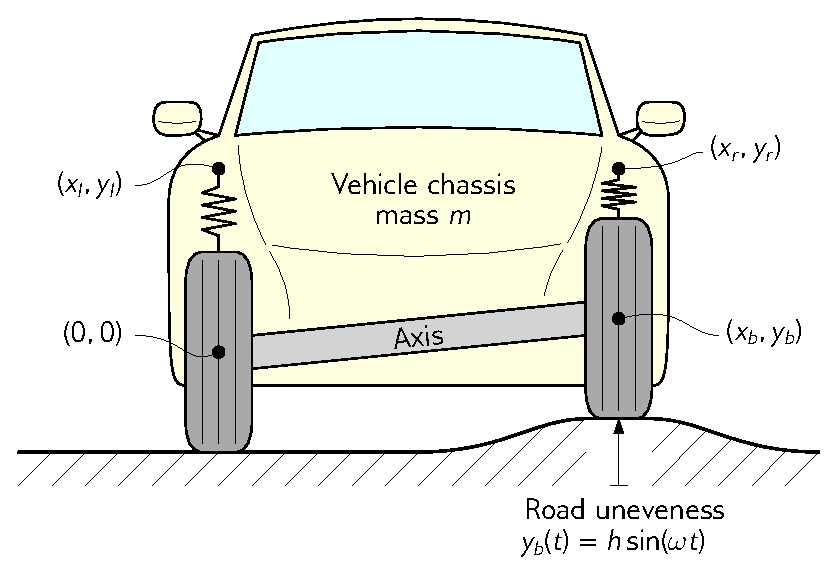
\includegraphics[width=\textwidth]{figures/car_axis.eps}
    \end{column}
  \end{columns}
  \centering{\scriptsize\begin{tabular}{cccc}
    \multicolumn{4}{c}{\textbf{Car-Axis (Index-3) -- \acs{LU} Factorization}} \\
    \toprule
    \textbf{Original \acsp{DAE}} & \multicolumn{3}{c}{$\mF = 108\cf + 131\cm + 56\ca$ \quad $\mh = 0$} \\
    \midrule
    \textbf{Reduction step} & $\mE$ & $\mg$ & $\ma$ \\
    \midrule
    Index-3 \acsp{DAE} & $12\cm$ & $94\cf + 145\cm + 54\ca$ & $14\cf + 16\cm + 10\ca$ \\
    Index-2 \acsp{DAE} & $12\cm$ & $94\cf + 145\cm + 54\ca$ & $26\cf + 45\cm + 15\ca$ \\
    Index-1 \acsp{DAE} & $12\cm$ & $94\cf + 145\cm + 54\ca$ & $136\cf + 4\cd + 261\cm + 95\ca$ \\
    Index-0 \acsp{DAE} & $1060\cf + 38\cd + 1901\cm + 717\ca$ & $431\cf + 8\cd + 842\cm + 268\ca$ & $0$ \\
    \midrule
    \rowcolor{mycolor5!25}
    \textbf{Reduced \acsp{DAE}} & \multicolumn{3}{c}{$\mF = 896\cf + 4\cd + 1202\cm + 546\ca$ \quad $\mh = 176\cf + 4\cd + 322\cm + 120\ca$} \\
    \bottomrule \\[0.05em]
    %
    \multicolumn{4}{c}{\textbf{Car-Axis (Index-3) -- \acs{FFLU} Factorization}} \\
    \toprule
    \textbf{Original \acsp{DAE}} & \multicolumn{3}{c}{$\mF = 108\cf + 131\cm + 56\ca$ \quad $\mh = 0$} \\
    \midrule
    \textbf{Reduction step} & $\mE$ & $\mg$ & $\ma$ \\
    \midrule
    Index-3 \acsp{DAE} & $0$ & $94\cf + 8\cd + 150\cm + 54\ca$ & $14\cf + 21\cm + 10\ca$ \\
    Index-2 \acsp{DAE} & $0$ & $94\cf + 8\cd + 154\cm + 54\ca$ & $26\cf + 1\cd + 44\cm + 15\ca$ \\
    Index-1 \acsp{DAE} & $0$ & $94\cf + 8\cd + 155\cm + 54\ca$ & $136\cf + 6\cd + 4\cd + 261\cm + 95\ca$ \\
    Index-0 \acsp{DAE} & $1066\cf + 55\cd + 1888\cm + 717\ca$ & $431\cf + 18\cd + 851\cm + 268\ca$ & $0$ \\
    \midrule
    \rowcolor{mycolor2!25}
    \textbf{Reduced \acsp{DAE}} & \multicolumn{3}{c}{$\mF = 1549\cf + 73\cd + 2765\cm + 1011\ca$ \quad $\mh = 176\cf + 7\cd + 326\cm + 120\ca$} \\
    \bottomrule
  \end{tabular}}
\end{frame}

\begin{frame}{Application Fields and Performance}{Expression Swell}
  \begin{columns}
    \centering
    \begin{column}[c]{0.7\textwidth}
      \hic{And when strong expression swell arise \dots}
    \end{column}
    \begin{column}[c]{0.22\textwidth}
      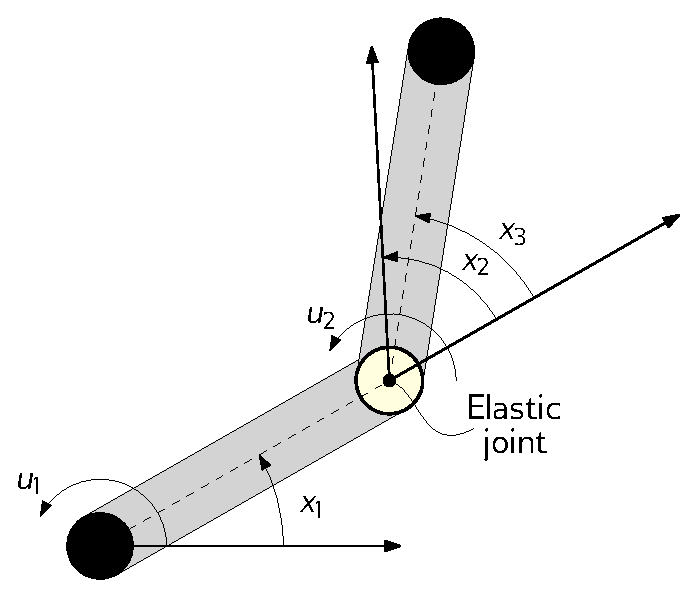
\includegraphics[width=\textwidth]{figures/robotic_arm.eps}
    \end{column}
  \end{columns}
  \hspace{-0.5em}
  \centering{\scriptsize\begin{tabular}{cccc}
    \multicolumn{4}{c}{\textbf{Robotic Arm (Index-5)}} \\
    \toprule
    \textbf{Original \acsp{DAE}} & \multicolumn{3}{c}{$\mF = 125\cf + 19\cd + 56\cm + 64\ca$ \quad $\mh = 0$} \\
    \midrule
    \textbf{Reduction step} & $\mE$ & $\mg$ & $\ma$ \\
    \midrule
    Index-5 \acsp{DAE} & $0$ & $66\cf + 3\cd + 50\cm + 35\ca$ & $16\cf + 12\ca$ \\
    Index-4 \acsp{DAE} & $0$ & $66\cf + 3\cd + 50\cm + 35\ca$ & $24\cf + 6\cm + 14\ca$ \\
    Index-3 \acsp{DAE} & $0$ & $66\cf + 3\cd + 50\cm + 35\ca$ & $162\cf + 2\cd + 138\cm + 114\ca$ \\
    Index-2 \acsp{DAE} & $14\cf + 2\cd + 6\cm + 6\ca$ & $372\cf + 4\cd + 375\cm + 253\ca$ & $972\cf + 1\cd + 1062\cm + 770\ca$ \\
    \rowcolor{mycolor2!25}
    Index-1 \acsp{DAE} & $14\cf + 2\cd + 6\cm + 6\ca$ & $372\cf + 4\cd + 375\cm + 253\ca$ & $\star (6.5\cf + 5.6\cm + 1.8\ca)\!\cdot\!10^{6} + 4\cd$ \\
    \rowcolor{mycolor2!25}
    Index-0 \acsp{DAE} & $\star (8.3\cf + 7.1\cm + 2.3\ca)\!\cdot\!10^{7} + 58\cd$ & $(2.4\cf + 2.0\cm + 0.9\ca)\!\cdot\!10^{6} + 8\cd$ & $0$ \\
    \midrule
    \rowcolor{mycolor2!25}
    \textbf{Reduced \acsp{DAE}} & \multicolumn{3}{c}{$\star \mF = (8.6\cf + 7.3\cm + 2.4\ca)\!\cdot\!10^{7} + 66\cd$ \quad $\star \mh = (6.5\cf + 5.6\cm + 1.8\ca)\!\cdot\!10^{6} + 7\cd$} \\
    \bottomrule
    \end{tabular}}
\end{frame}

\begin{frame}{Application Fields and Performance}{Expression Swell Mitigation}
  \vspace{-2.0em}
  \hic{\dots hierarchical representation does the job}
  \vspace{-0.5em}
  \centering{\scriptsize\begin{tabular}{cccc}
    \multicolumn{4}{c}{\textbf{Robotic Arm (Index-5)}} \\
    \toprule
    \textbf{Original \acsp{DAE}} & \multicolumn{3}{c}{$\mFv = 125\cf + 19\cd + 56\cm + 64\ca$ \quad $\mhv = 0$ \quad $\mv = 0$} \\
    \midrule
    \textbf{Reduction step} & $\mEv$ & $\mgv$ & $\mav$ \\
    \midrule
    Index-5 \acsp{DAE} & $0$ & $66\cf + 3\cd + 50\cm + 35\ca$ & $16\cf + 12\ca$ \\
    Index-4 \acsp{DAE} & $0$ & $66\cf + 3\cd + 50\cm + 35\ca$ & $24\cf + 6\cm + 14\ca$ \\
    Index-3 \acsp{DAE} & $0$ & $66\cf + 3\cd + 50\cm + 35\ca$ & $162\cf + 2\cd + 138\cm + 114\ca$ \\
    Index-2 \acsp{DAE} & $14\cf + 2\cd + 6\cm + 6\ca$ & $66\cf + 1\cv + 3\cd + 51\cm + 35\ca$ & $1\cm + 1\cv$ \\
    \rowcolor{mycolor5!25}
    Index-1 \acsp{DAE} & $2\cv + 1\ca$ & $66\cf + 1\cv + 3\cd + 51\cm + 35\ca$ & \cellcolor{mycolor5!25}$9\cf + 4\cv + 2\cd + 8\cm + 5\ca$ \\
    \rowcolor{mycolor5!25}
    Index-0 \acsp{DAE} & $7\cv + 1\cd + 2\cm + 2\ca$ & \cellcolor{mycolor5!25}$66\cf + 2\cv + 3\cd + 52\cm + 35\ca$ & $0$ \\
    \midrule
    \rowcolor{mycolor5!25}
    \textbf{Reduced \acsp{DAE}} & \multicolumn{3}{c}{$\mFv = 90\cf + 9\cv + 4\cd + 63\cm + 48\ca$ \quad $\mhv = 202\cf + 5\cv + 4\cd + 141\cm + 130\ca$} \\
    \bottomrule \\[-0.65em]
  \end{tabular}}
  \begin{columns}
    \centering
    \begin{column}[c]{0.5\textwidth}
      \centering{\scriptsize\begin{tabular}{cc}
        \multicolumn{2}{c}{Hierarchical representation details (29 veils)} \\
        \toprule
        \textbf{Reduction step} & $\mv$ \\
        \midrule
        Index-5 \acsp{DAE} & $0$ \\
        Index-4 \acsp{DAE} & $0$ \\
        Index-3 \acsp{DAE} & $0$ \\
        Index-2 \acsp{DAE} & $1278\cf + 3\cv + 6\cd + 1319\cm + 918\ca$ \\
        \rowcolor{mycolor3!25}
        Index-1 \acsp{DAE} & $8401\cf + 20\cv + 24\cd + 9451\cm + 6095\ca$ \\
        \rowcolor{mycolor3!25}
        Index-0 \acsp{DAE} & $37010\cf + 558\cv + 56\cd + 45087\cm + 28665\ca$ \\
        \midrule
        \rowcolor{mycolor3!25}
        \textbf{Reduced \acsp{DAE}} & $\mv = 37010\cf + 558\cv + 56\cd + 45087\cm + 28665\ca$ \\
        \bottomrule
      \end{tabular}}
    \end{column}
    \hspace{1.0em}
    \begin{column}[c]{0.215\textwidth}
      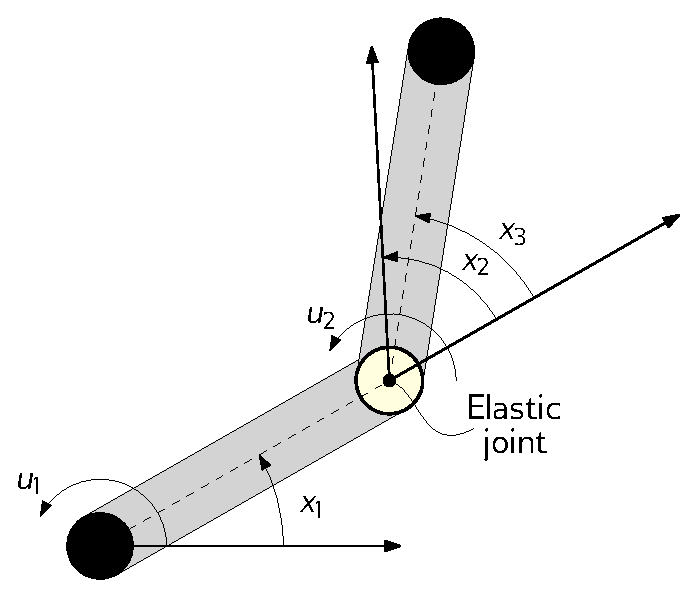
\includegraphics[width=\textwidth]{figures/robotic_arm.eps}
    \end{column}
  \end{columns}
\end{frame}

\begin{frame}{Application Fields and Performance}{Numerical Stability}
  \vspace{-2.0em}\begin{columns}
    \centering
    \begin{column}[c]{0.3\textwidth}
      \hic{Numerical\vphantom{y} stability is preserved \dots}
      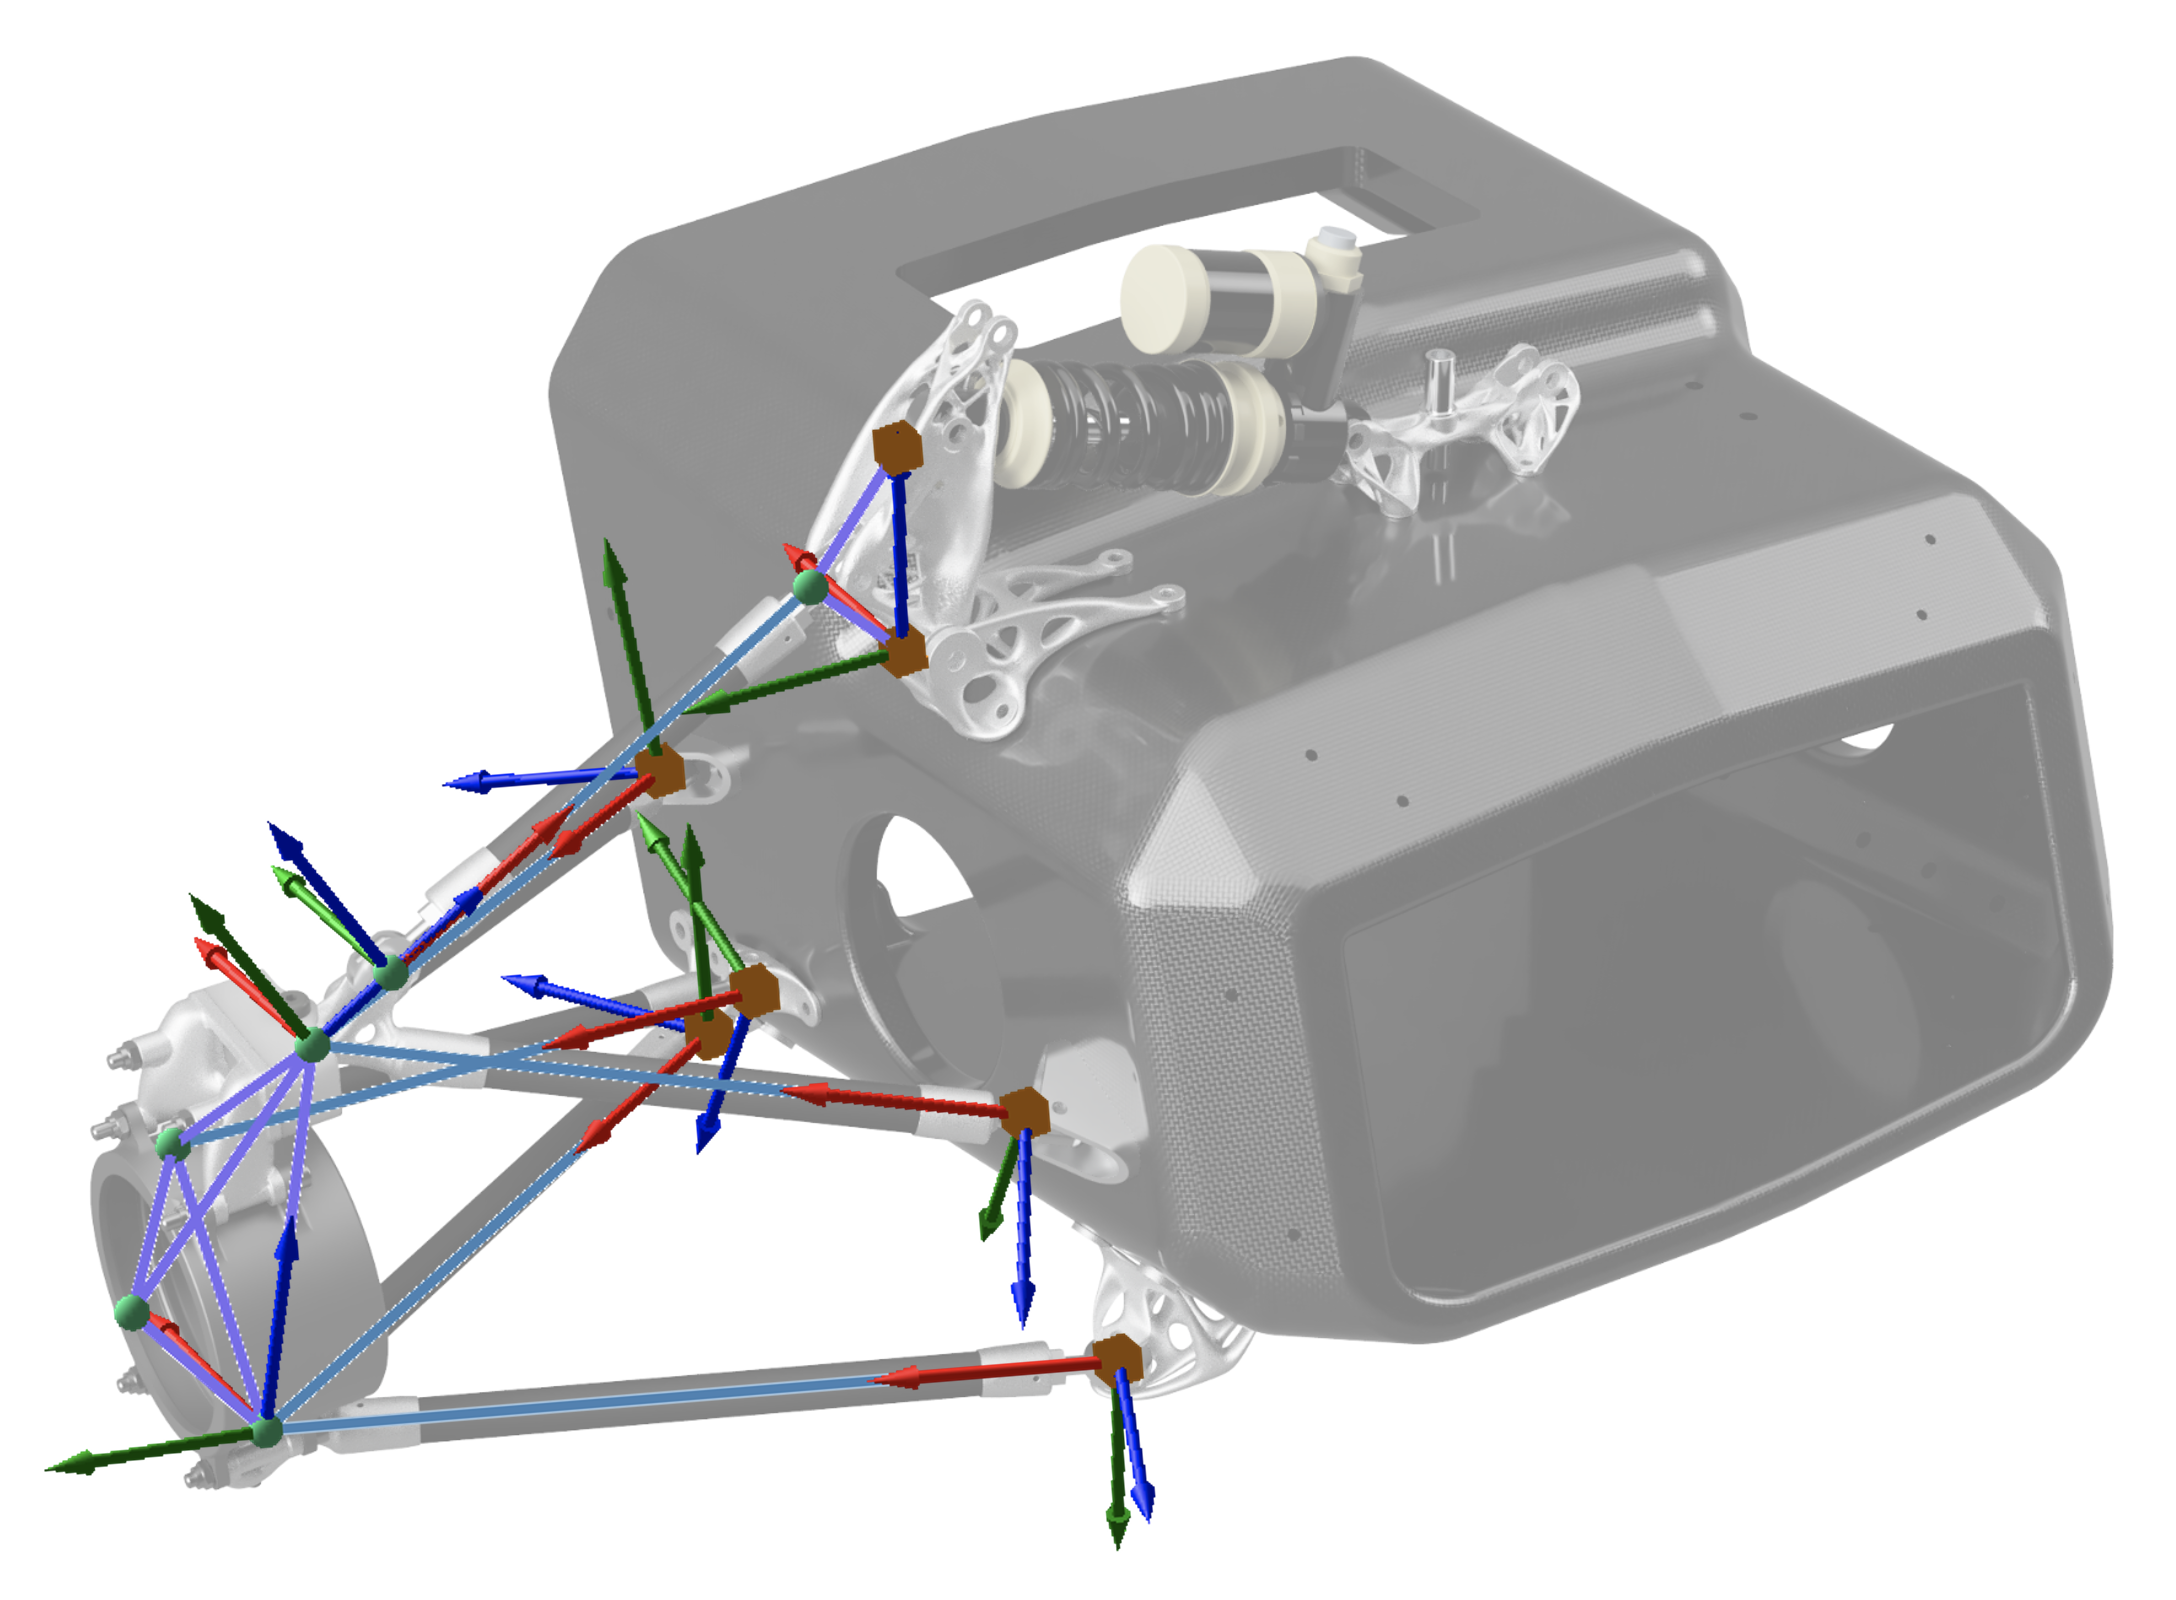
\includegraphics[width=\textwidth]{figures/fade_overview.png}
      \hic{\dots but not guaranteed}
    \end{column}
    \begin{column}[c]{0.7\textwidth}
      \vspace{1em}\small{
\begin{tikzpicture}

\begin{axis}[%
  minor tick num=1,
  minor grid style={dashed, line width=.1pt, draw=gray!45},
  major grid style={line width=.2pt, draw=gray!60},
  width=8.0cm,
  height=2.0cm,
  at={(0.0in,0.0in)},
  scale only axis,
  xmin=0,
  xmax=80,
  xticklabels=\empty,
  xlabel style={font=\color{black}},
  ymin=-3.5,
  ymax=3.5,
  ylabel shift = 0.31cm,
  ylabel style={font=\color{black}},
  ylabel={$z$ (\USI{\centi\meter})},
  axis background/.style={fill=none},
  xmajorgrids,
  xminorgrids,
  ymajorgrids,
  yminorgrids
]
\addplot[color=mycolor1, line width=0.8pt, forget plot]
  table[row sep=crcr]{%
0	-0.277154470527796\\
0.0345882407885706	-0.299442752220327\\
0.0691941739051554	-0.318274653937545\\
0.103790654936363	-0.335654836385291\\
0.138390399276118	-0.350371557532148\\
0.172990729409821	-0.365317407294444\\
0.207588587716144	-0.382913649511246\\
0.242189396030985	-0.400390783223761\\
0.276787636446035	-0.415096204408649\\
0.311387731209297	-0.428149198111488\\
0.345986691723649	-0.442081394855026\\
0.380586187286335	-0.456038602089787\\
0.415185581622751	-0.469044243035108\\
0.449784809184073	-0.48049311621278\\
0.484384291221631	-0.490300903099941\\
0.518983552545111	-0.49805162209923\\
0.553582986412253	-0.503675895969799\\
0.588182292762749	-0.508308033023003\\
0.622781664832205	-0.511699574791585\\
0.657381009541431	-0.514234589510118\\
0.691980387807863	-0.516361946475039\\
0.72657974998383	-0.519133617841885\\
0.761179071071826	-0.523196560215516\\
0.795778454348609	-0.528399675147753\\
0.830377811196801	-0.535635815122915\\
0.864977169973516	-0.544056937481902\\
0.899576536696105	-0.558036397026773\\
0.934175888700616	-0.574297358259432\\
0.968775246957456	-0.5840099888828\\
1.00337461208462	-0.588794561610456\\
1.0379739487237	-0.589907272041928\\
1.07257329782181	-0.590660060699663\\
1.10717267095451	-0.59356895772846\\
1.14177202042456	-0.596174553620732\\
1.17637136503327	-0.59850996344756\\
1.21097071970166	-0.599817538838487\\
1.24557009444157	-0.600102936397773\\
1.28016943063923	-0.600414084109568\\
1.31476881887339	-0.600596430179093\\
1.34936821120442	-0.601253328962889\\
1.38396750786284	-0.602730867618068\\
1.41856685423327	-0.604719737754525\\
1.45316620563869	-0.60684703131873\\
1.48776559414576	-0.609217534445877\\
1.52236493624834	-0.611229672141619\\
1.55696431064692	-0.612746768732791\\
1.59156367360511	-0.615145364205455\\
1.62616301164522	-0.618332384110029\\
1.66076239497077	-0.622205163776859\\
1.69536172759775	-0.626372623525226\\
1.72996107482685	-0.630736873139406\\
1.7645604352467	-0.636175347852411\\
1.79915979893981	-0.64177689939463\\
1.83375919958795	-0.64663925546318\\
1.86835850469035	-0.650510992097325\\
1.90295788396199	-0.654325360659005\\
1.93755725450998	-0.658640630831422\\
1.97215660287566	-0.662401557980932\\
2.00675594118731	-0.665280013663433\\
2.04135528034861	-0.667884064124502\\
2.07595464810064	-0.67106300436337\\
2.11055402554662	-0.675345386895426\\
2.14515333255837	-0.681410418109285\\
2.17975266519694	-0.688398754615283\\
2.21435210953785	-0.695138551621582\\
2.24895146869019	-0.701212014540353\\
2.28355082657261	-0.707138672041505\\
2.3181501776242	-0.713831334242834\\
2.35274948563224	-0.720195085152392\\
2.38734889277826	-0.726099943870384\\
2.42194824169299	-0.732368402888348\\
2.45654760516451	-0.739284007487556\\
2.49114698071954	-0.747118873683\\
2.525746325308	-0.755476551691553\\
2.56034564152321	-0.76384052616579\\
2.59494497202408	-0.772208357137752\\
2.62954438593392	-0.781497982776647\\
2.66414371710205	-0.791409879530636\\
2.69874304857414	-0.800722026750475\\
2.73334244293772	-0.809643561321705\\
2.76794178388125	-0.818224723937519\\
2.80254116244336	-0.826372755837276\\
2.83714049671265	-0.834997255692166\\
2.87173985374807	-0.84394562765705\\
2.90633925340285	-0.852648891263086\\
2.94093867237209	-0.861412324310637\\
2.97553800113202	-0.870294992839868\\
3.0101373085465	-0.879177418957236\\
3.04473666764481	-0.888111335466973\\
3.0793359639325	-0.897473387562994\\
3.11393531927037	-0.906895842495173\\
3.14853471781257	-0.915566112601415\\
3.18313412218822	-0.923700963481305\\
3.21773337799291	-0.932120033430112\\
3.25233273828374	-0.940510785815751\\
3.28693209817599	-0.948321800488766\\
3.32153151621568	-0.95617579200597\\
3.3561308234352	-0.964240440343253\\
3.39073016293086	-0.972222121762475\\
3.42532960430035	-0.980516149981195\\
3.45992894684792	-0.988849045161103\\
3.49452826507548	-0.996433379948586\\
3.52912767084389	-1.00378043837478\\
3.56372697423673	-1.01103025323463\\
3.5983263514209	-1.01805465896425\\
3.63292573128913	-1.02471278325558\\
3.66752504125867	-1.03067300282685\\
3.7021244011534	-1.03681063450781\\
3.73672383088158	-1.04322929480058\\
3.77132321330692	-1.0496959301399\\
3.80592249175793	-1.05576679780259\\
3.84052184036334	-1.0604488550242\\
3.87512122306321	-1.06406024713933\\
3.90972055173965	-1.06754230554122\\
3.94431999203624	-1.07122830593711\\
3.97891932495401	-1.07577574028434\\
4.0135186596972	-1.08123533971583\\
4.04811800309016	-1.08668721055165\\
4.08271737018387	-1.09247589464429\\
4.11731676085916	-1.09896598053001\\
4.15191605825494	-1.10569809433619\\
4.18651547389976	-1.11257494453942\\
4.22111479536817	-1.11930390353537\\
4.25571421197176	-1.12527897054676\\
4.29031354536852	-1.13042465094677\\
4.32491284646932	-1.13533903733204\\
4.35951221487519	-1.14076218841362\\
4.39411155470318	-1.14590048306474\\
4.42871088364808	-1.15022588238983\\
4.46331027169934	-1.15359396609878\\
4.49790969796062	-1.15587494719864\\
4.53250901086568	-1.15828450111279\\
4.56710835183398	-1.16067090443925\\
4.60170766339017	-1.1625977576443\\
4.63630704566509	-1.16474475348104\\
4.67090642369396	-1.16757528976894\\
4.70550582199882	-1.1720977709385\\
4.74010516937966	-1.17874741388992\\
4.77470455395202	-1.18636709100066\\
4.80930394104339	-1.19311284999114\\
4.84390309448492	-1.19882759367674\\
4.87850245830094	-1.20420966792802\\
4.91310193131662	-1.20741630267395\\
4.9477012604259	-1.21065165417374\\
4.98230073511971	-1.21523782958053\\
5.01690009376786	-1.21807202102125\\
5.05149933068316	-1.21992893848053\\
5.08609871558529	-1.22109546560095\\
5.12069798500917	-1.22111551530351\\
5.15529739542279	-1.22038192625363\\
5.18989675756718	-1.21715568231597\\
5.2244961369571	-1.21230040887358\\
5.25909548491879	-1.20671546197247\\
5.29369486139244	-1.20129845876072\\
5.32829433451557	-1.19806710236807\\
5.36289352996098	-1.19653040922985\\
5.39749296312739	-1.19944107340113\\
5.43209218238676	-1.20441517147731\\
5.46669153260357	-1.20752591199499\\
5.50129108926218	-1.21217955484285\\
5.53589037243282	-1.21908146467842\\
5.57048976288035	-1.22664814437308\\
5.60508906196475	-1.23398487363374\\
5.63968844366828	-1.2400653151376\\
5.67428779812231	-1.24528878763436\\
5.70888715616292	-1.25163716850821\\
5.74348652150097	-1.25843186047222\\
5.77808589718709	-1.26387004341182\\
5.81268515708174	-1.2688845206892\\
5.8472845360341	-1.27313945987341\\
5.88188402769357	-1.27629386889479\\
5.91648331347069	-1.27835153773276\\
5.95108255651113	-1.2788235284958\\
5.98568199729077	-1.27810425957437\\
6.02028141712278	-1.27627653781024\\
6.0548807501494	-1.27241703292619\\
6.08948009161315	-1.26528848115817\\
6.12407939058931	-1.25455240689917\\
6.15867871433572	-1.23986813640573\\
6.19327812899653	-1.2231532025333\\
6.22787750077383	-1.20368193195156\\
6.26247692990338	-1.18940875009363\\
6.29707610232678	-1.23084340547784\\
6.33167541731734	-1.33819897488052\\
6.36627495007784	-1.34879618309902\\
6.40087431562739	-1.18462760300861\\
6.43547361364151	-1.02335697498827\\
6.4700730387972	-0.942206659664244\\
6.50467231720328	-0.867943675007549\\
6.53927159880973	-0.760952956260799\\
6.57387108612595	-0.64367282504425\\
6.60847043532192	-0.541669192124791\\
6.64306981157613	-0.448401686672448\\
6.67766910562262	-0.361969922019123\\
6.71226843821673	-0.28647123977863\\
6.74686786193811	-0.219291077603109\\
6.78146720738271	-0.154730935928699\\
6.81606661691788	-0.0915835020364575\\
6.85066603172181	-0.0367093726799272\\
6.88526518901969	0.00577072892694597\\
6.91986465428691	0.0396630793883718\\
6.95446400851418	0.0656101068238268\\
6.98906341791564	0.082249507683585\\
7.02366276872973	0.0920003492099142\\
7.05826192661799	0.0954413867438136\\
7.09286148129173	0.0925242072257054\\
7.1274608307713	0.082115322535728\\
7.16206012265865	0.0664906162328949\\
7.1966593865526	0.0495558432637211\\
7.23125878220833	0.0289958087751702\\
7.26585804677176	0.0058093876249915\\
7.30045752503653	-0.0189228585685486\\
7.33505704348135	-0.0485601385664253\\
7.36965643133652	-0.0799643974065845\\
7.40425584543158	-0.110727622765666\\
7.43885497198487	-0.141771989204584\\
7.47345432741726	-0.170950702796976\\
7.50805367859434	-0.198670075337309\\
7.54265306921247	-0.225370787359963\\
7.57725241066315	-0.248467490430826\\
7.61185163359891	-0.269483879044924\\
7.64645112509188	-0.290763357739154\\
7.68105055182334	-0.310982272018867\\
7.71564977694563	-0.3277400836629\\
7.75024913986982	-0.339652412413291\\
7.78484869949597	-0.348712211751889\\
7.81944794856821	-0.35714392773753\\
7.8540472084544	-0.363294778841017\\
7.88864660214664	-0.365444229299819\\
7.92324596230653	-0.364019151166972\\
7.95784532849396	-0.362403487961857\\
7.9924447387828	-0.362599695258359\\
8.02704399366204	-0.366686248143572\\
8.06164333808838	-0.378700437574378\\
8.09624279070773	-0.396302786674874\\
8.13084210467614	-0.416616247139365\\
8.16544154684889	-0.449917522253174\\
8.20004086202665	-0.572638438396589\\
8.23464026639844	-0.822449258022756\\
8.26923948313222	-1.06122319340796\\
8.30383885709299	-1.17723646878306\\
8.33843829497494	-1.1490390803695\\
8.37303757507769	-1.03091052982542\\
8.40763697346256	-0.961826587195569\\
8.44223637812242	-0.949594295243189\\
8.47683559014479	-0.920812286049907\\
8.51143501179526	-0.883921352568853\\
8.54603437822958	-0.872407971649602\\
8.5806336687454	-0.86632078103189\\
8.61523317309015	-0.847223396326399\\
8.64983253971842	-0.830795375037061\\
8.68443175120546	-0.829881313100192\\
8.71903104081348	-0.835144193789303\\
8.75363054816198	-0.835192904119458\\
8.78822985356296	-0.83443023822185\\
8.82282919727061	-0.838741592442907\\
8.85742877415666	-0.847449107359216\\
8.89202805238453	-0.853977468080783\\
8.92662743673166	-0.856283488513124\\
8.96122673412624	-0.859229593182928\\
8.99582595140102	-0.863007688147027\\
9.03042538819582	-0.865925999893782\\
9.06502478820051	-0.868155224642744\\
9.09962396486308	-0.869503273485045\\
9.13422331362283	-0.868152095074898\\
9.1688228845378	-0.86143675994837\\
9.20342234614905	-0.852035269558749\\
9.23802166602345	-0.842357162444307\\
9.27262099358278	-0.831190789152922\\
9.30722047039201	-0.820646900918251\\
9.34181962232666	-0.812220279864884\\
9.37641891430065	-0.808673725327727\\
9.411018334881	-0.818826629581199\\
9.44561766114339	-0.843023290473408\\
9.48021702921742	-0.863591786210441\\
9.51481637967015	-0.881690033527305\\
9.54941560079428	-0.902728956043464\\
9.58401522551847	-0.919428256680752\\
9.61861448513802	-0.935148297131444\\
9.65321376945465	-0.951233604538834\\
9.68781322786361	-0.967359737608553\\
9.72241246406336	-0.982140397417811\\
9.75701191374827	-0.992959966795523\\
9.79161131412046	-1.00226682900302\\
9.82621056365065	-1.01219030391695\\
9.86080990667173	-1.02082422344938\\
9.89540932270542	-1.02316924845611\\
9.93000868467231	-1.01647079153086\\
9.96460810421018	-1.00425286836785\\
9.99920749184953	-0.98845861957973\\
10.0338066806869	-0.965686642455052\\
10.0684060071147	-0.93831776214057\\
10.1030055136655	-0.914602526202596\\
10.1376048665068	-0.902528158038632\\
10.1722040578497	-0.901435725536956\\
10.2068035323449	-0.902194109986931\\
10.2414028674657	-0.895883223013136\\
10.2760022312573	-0.882623605195462\\
10.3106018326505	-0.871374030448333\\
10.3452010516906	-0.868603916635632\\
10.3798002796614	-0.875234394104393\\
10.4143994969271	-0.887172568593206\\
10.4489989553989	-0.894434431803937\\
10.4835984576344	-0.890215104883679\\
10.5181976588749	-0.879608902780882\\
10.5527970496486	-0.878525044658138\\
10.5873964025476	-0.888946276268787\\
10.62199582328	-0.881426448134015\\
10.656595238111	-0.864934461209182\\
10.6911944900742	-0.863001928776805\\
10.7257938836803	-0.882987507345506\\
10.760393396858	-0.924448188152568\\
10.7949926046609	-0.960752457904115\\
10.8295919185552	-0.989507435457535\\
10.8641913063098	-1.01266219818323\\
10.8987906058103	-1.02933708967999\\
10.9333900893917	-1.03723152761011\\
10.9679893354806	-1.04460199486609\\
11.0025888829107	-1.06863696343061\\
11.0371882466516	-1.09642453193956\\
11.0717874270741	-1.12045548628305\\
11.1063869592157	-1.1443796958837\\
11.1409861357495	-1.16604500073337\\
11.1755855465482	-1.18167868055819\\
11.2101848773956	-1.1863355700874\\
11.2447841231765	-1.17912696443186\\
11.2793836287216	-1.16008237517345\\
11.3139828913666	-1.11617749907265\\
11.3485821937631	-1.06093780071647\\
11.3831816741482	-1.01662122531993\\
11.4177810890384	-0.972493811757802\\
11.4523803854056	-0.923436181025619\\
11.4869796775207	-0.867417766682177\\
11.521578876686	-0.81644093709986\\
11.5561782623931	-0.78249945579468\\
11.5907776610381	-0.762773198666153\\
11.6253770521733	-0.758073166625317\\
11.6599766415132	-0.764675727208386\\
11.6945760880389	-0.762314468839251\\
11.729175451923	-0.745031410282188\\
11.7637746211036	-0.749969213037716\\
11.7983740264102	-0.773655263975295\\
11.8329735243236	-0.796878064289744\\
11.8675727260044	-0.82272741712574\\
11.902172167364	-0.840439590077399\\
11.9367713837392	-0.854054799849457\\
11.9713706771907	-0.839106623565097\\
12.0059702138619	-0.802287822308054\\
12.0405695149233	-0.790320246091314\\
12.0751688842601	-0.784713069939266\\
12.1097682276169	-0.774441111951774\\
12.1443676318791	-0.769463684343319\\
12.1789669009118	-0.772877798745467\\
12.2135660234401	-0.775032166661371\\
12.2481657314605	-0.765732292000634\\
12.2827650524643	-0.755966308284553\\
12.3173642250466	-0.750726676948876\\
12.3519635544158	-0.75406492519827\\
12.3865630375101	-0.764911461954232\\
12.4211623572928	-0.779425223289335\\
12.4557615536817	-0.803562764826418\\
12.4903610153418	-0.833931021397438\\
12.5249602669955	-0.858773221777742\\
12.5595596369199	-0.868785386075471\\
12.5941591720121	-0.867452781169697\\
12.6287585209857	-0.86198978216919\\
12.6633579385331	-0.847590933669007\\
12.6979573260335	-0.8335486469326\\
12.7325566678903	-0.822806886613348\\
12.7671560596487	-0.808852811900121\\
12.8017551794345	-0.802224313448063\\
12.8363545839707	-0.806978964539798\\
12.8709540622912	-0.820501802598189\\
12.9055534265316	-0.847108376804148\\
12.9401525601374	-0.887453130327609\\
12.9747520951941	-0.940871030492169\\
13.0093516635386	-1.00808389834362\\
13.0439510202357	-1.08215181651223\\
13.0785502377239	-1.15794688004242\\
13.1131495632647	-1.2311516534443\\
13.1477490809098	-1.28758571005331\\
13.1823484028361	-1.33705625397892\\
13.2169479139533	-1.38340065978418\\
13.2515471564861	-1.43318096824413\\
13.2861463319847	-1.4984319467909\\
13.3207457916155	-1.56173893146116\\
13.3553452769694	-1.55691438273093\\
13.3899445034642	-1.41635875996875\\
13.4245439261465	-1.25007822308762\\
13.459143584261	-1.16478110997829\\
13.4937425518845	-1.09638150095386\\
13.5283421065042	-1.0090344154594\\
13.5629413835614	-0.941462697016168\\
13.5975403347865	-0.910449700353225\\
13.6321397740416	-0.881566457463645\\
13.6667390580758	-0.844556047975811\\
13.7013384686137	-0.82125800845112\\
13.7359379468641	-0.810531219185484\\
13.7705373595658	-0.786654625670896\\
13.8051364053195	-0.745864081291173\\
13.8397359663883	-0.706932894127285\\
13.8743353646947	-0.669052505669054\\
13.9089348938638	-0.635867085218061\\
13.9435339652332	-0.610015454497975\\
13.9781333887056	-0.58633742036697\\
14.0127328696766	-0.559898929732228\\
14.0473319572604	-0.527701439848249\\
14.0819315490222	-0.490910086600432\\
14.1165306257995	-0.447617013708404\\
14.1511299670303	-0.40365511854776\\
14.1857293936557	-0.353664193841211\\
14.2203288063146	-0.299484831027988\\
14.2549283748504	-0.257825336496995\\
14.2895278381931	-0.229333968175735\\
14.3241269880153	-0.212911581433606\\
14.3587262265656	-0.20420459885156\\
14.3933257869082	-0.206515765429285\\
14.4279249978875	-0.217455378199291\\
14.4625245585029	-0.241759228049671\\
14.4971237430479	-0.289203847562042\\
14.531723060386	-0.291697075486572\\
14.5663228352391	-0.230219123164324\\
14.6009217786413	-0.167519830502916\\
14.6355213790572	-0.109528056460634\\
14.670120730097	-0.0808737553361943\\
14.7047198808084	-0.0894277834246893\\
14.7393194651601	-0.112428246512578\\
14.7739184809631	-0.165892371430951\\
14.8085176746697	-0.196394515040613\\
14.8431171851589	-0.178067761908585\\
14.8777166013357	-0.137136131550325\\
14.9123161766749	-0.0605939050772997\\
14.9469155385466	0.0335972688890629\\
14.9815147879562	0.101499859762361\\
15.0161142127177	0.117852828389139\\
15.0507136665452	0.0570676941397757\\
15.0853129498827	-0.0298879028994808\\
15.1199121880127	-0.0283494867120926\\
15.1545115807568	0.0411733850652268\\
15.1891108414578	0.122806628619693\\
15.2237103169619	0.161371327130999\\
15.2583097817989	0.175826405624843\\
15.2929089062241	0.161894738114146\\
15.3275084834808	-0.0607442844905687\\
15.362107664082	-0.271732261223956\\
15.3967069949685	-0.313905941509102\\
15.4313065221914	-0.356537805780038\\
15.4659055189476	-0.377751665448994\\
15.5005050896411	-0.37445197752759\\
15.5351045353104	-0.362506545229682\\
15.5697039193504	-0.364206768594\\
15.604303011334	-0.390216884954844\\
15.638902491988	-0.414092641521085\\
15.6735019264685	-0.441325948335616\\
15.7081014759677	-0.471989140163445\\
15.7427011510901	-0.502462022786093\\
15.7773001120248	-0.538541284546348\\
15.8118992597275	-0.561811411233484\\
15.8464987218374	-0.561037512473084\\
15.8810980914076	-0.538204207536194\\
15.9156975422668	-0.510293868882616\\
15.9502967761027	-0.50038521513667\\
15.9848958873371	-0.494244438618588\\
16.0194955411046	-0.509024325980226\\
16.054094940063	-0.548335545104253\\
16.088694164671	-0.589263223752556\\
16.1232933019522	-0.6267031346536\\
16.1578926032285	-0.643243004569782\\
16.1924922834276	-0.644393457163561\\
16.2270915919241	-0.623369024895595\\
16.2616907160304	-0.57514189551795\\
16.2962902983729	-0.544509039104765\\
16.3308898029491	-0.5396858919134\\
16.3654892586526	-0.555405115711147\\
16.4000884283055	-0.593866414571834\\
16.4346879285504	-0.631440658079518\\
16.469287044783	-0.677567887749372\\
16.5038865317471	-0.712764452708625\\
16.538486007397	-0.715340262598471\\
16.5730850672267	-0.709468824397577\\
16.6076846108219	-0.690002678157031\\
16.6422839889895	-0.673635373932785\\
16.6768832919448	-0.670387907739259\\
16.7114825425395	-0.682821896547137\\
16.7460821641792	-0.716980672106396\\
16.7806813211623	-0.746249641852686\\
16.8152805800903	-0.770391477347387\\
16.8498802485642	-0.788864086175195\\
16.8844794077612	-0.797958668325952\\
16.9190791081002	-0.797685654543018\\
16.9536781656898	-0.777824646665529\\
16.9882772392083	-0.757381402131782\\
17.0228767815076	-0.746623595686116\\
17.0574759392241	-0.741964019648952\\
17.0920754937805	-0.741946991170064\\
17.1266750197781	-0.744403251973047\\
17.161274492455	-0.754715439058604\\
17.1958737111493	-0.764082528029997\\
17.2304728623066	-0.765793452999461\\
17.2650724043098	-0.761317051778676\\
17.299671712895	-0.751963323529764\\
17.3342712743964	-0.749503021113287\\
17.3688704386436	-0.756985932125256\\
17.4034697893649	-0.773124761750452\\
17.4380693761089	-0.800074841281428\\
17.4726682001892	-0.830791154759727\\
17.5072675498504	-0.862788857790542\\
17.5418672775023	-0.891396095087146\\
17.5764666415104	-0.913910007842891\\
17.6110658006677	-0.925431891884648\\
17.645665164881	-0.919742247815933\\
17.6802642933395	-0.906554313165117\\
17.7148637697468	-0.895373893058724\\
17.7494635245265	-0.893467643677096\\
17.7840628323281	-0.904420739240752\\
17.8186621604585	-0.928978348369083\\
17.8532614321426	-0.957122980010511\\
17.8878607860482	-0.983244873915642\\
17.9224603044061	-1.0011326047434\\
17.9570596404675	-1.00359778192995\\
17.9916585821376	-1.00187311485619\\
18.0262580216671	-0.97648412933177\\
18.0608572080554	-0.943892050335216\\
18.0954569063364	-0.938851025661605\\
18.1300564222227	-0.942607746644281\\
18.164655761731	-0.954800790683338\\
18.1992549049389	-0.970983795148928\\
18.2338541202075	-0.991251906268564\\
18.2684537711743	-1.0104145349008\\
18.3030529148988	-1.01123729864191\\
18.3376523913822	-0.998649594425133\\
18.3722517960644	-0.969085168395942\\
18.4068511786035	-0.939259311295249\\
18.4414504187521	-0.92277666803551\\
18.4760497764527	-0.913361552852993\\
18.5106493604754	-0.920013304196923\\
18.5452482639784	-0.941359682121287\\
18.5798480929407	-0.964919198360614\\
18.6144472652169	-0.974687110739647\\
18.6490465426018	-0.963188697288497\\
18.6836465110028	-0.950205577824076\\
18.7182454697345	-0.947081664186825\\
18.7528445790825	-0.950399581532138\\
18.7874444173831	-0.965666398580003\\
18.8220432576653	-0.98753586508197\\
18.8566425196592	-1.00797835165217\\
18.8912423580979	-1.02368145092603\\
18.9258413688678	-1.03607367347019\\
18.9604408725981	-1.04465282093322\\
18.9950402143781	-1.04555406185359\\
19.029639426859	-1.04181041596431\\
19.0642390319283	-1.03321739405026\\
19.0988382356936	-1.02469573456942\\
19.1334376337387	-1.01528435210009\\
19.1680371336219	-0.992636200052963\\
19.2026367003948	-0.967428142308152\\
19.2372356360372	-0.945528933825096\\
19.2718350495433	-0.92084352970532\\
19.3064344933655	-0.896377043205643\\
19.3410336447412	-0.875062933368095\\
19.3756331846275	-0.859338523822253\\
19.4102320778329	-0.841535901181667\\
19.444831809153	-0.815213031437903\\
19.4794314936	-0.791849181388432\\
19.5140304870792	-0.778069829589084\\
19.5486299198975	-0.779545966623857\\
19.5832294257586	-0.797772585988407\\
19.6178289544304	-0.821907914028419\\
19.6524276479906	-0.857238703131313\\
19.6870270358036	-0.889412718098892\\
19.721626809465	-0.904792104114185\\
19.7562258769593	-0.908062979642915\\
19.7908253766765	-0.909843380647757\\
19.8254249251297	-0.904204640396913\\
19.8600240712799	-0.893152543694994\\
19.8946231756067	-0.901148198899979\\
19.9292228844387	-0.921094016514212\\
19.9638221195471	-0.942583088276649\\
19.9984215089282	-0.960405718279031\\
20.0330209792948	-0.979427480409151\\
20.0676200937033	-0.999574478867743\\
20.1022197988766	-1.0106990236615\\
20.1368188481544	-1.01491306055883\\
20.1714183399469	-1.01489495729559\\
20.2060178769946	-1.01738695435019\\
20.2406172812693	-1.02261448840289\\
20.2752164989002	-1.02785584737125\\
20.309815823011	-1.03384885316125\\
20.3444150489721	-1.03865193099366\\
20.3790144107108	-1.03929318212488\\
20.4136135483928	-1.03410582680989\\
20.4482131446565	-1.01950773208434\\
20.4828124001344	-0.994514601613897\\
20.5174114732499	-0.966497486291046\\
20.5520117131395	-0.93059623662024\\
20.5866103744936	-0.896376332254686\\
20.6212097800417	-0.865924943216509\\
20.6558095157389	-0.829266944524851\\
20.6904089021338	-0.797234330106192\\
20.7250082109534	-0.768737235674383\\
20.7596074813499	-0.742087029201072\\
20.7942069189791	-0.716874591592909\\
20.8288061098149	-0.690747522470703\\
20.863405347173	-0.667275784200921\\
20.8980046175423	-0.636726514863203\\
20.9326039624701	-0.597065498498658\\
20.9672035471175	-0.55564905765968\\
21.001802846781	-0.519997696795454\\
21.0364021578111	-0.492737425447082\\
21.0710015114695	-0.469103383030731\\
21.1056010762977	-0.444162579359816\\
21.1402003081916	-0.415810979684164\\
21.1747993604864	-0.388827176879308\\
21.2093990215224	-0.36289666335767\\
21.2439984654491	-0.339007729186744\\
21.2785977116936	-0.313484765216079\\
21.313197118913	-0.283758953133517\\
21.3477966771773	-0.257033680861907\\
21.3823959228729	-0.23473005476021\\
21.4169951904524	-0.215369546210092\\
21.4515943517029	-0.195507380694182\\
21.4861939158909	-0.173684918081515\\
21.5207934807854	-0.151802851470462\\
21.5553926876145	-0.130027042069134\\
21.5899920088479	-0.106853663869105\\
21.6245911163896	-0.0777089627332972\\
21.6591904245888	-0.040389134223015\\
21.6937901986995	0.00186721613202323\\
21.728389213225	0.0455031905656433\\
21.7629889571347	0.090258488430775\\
21.7975884147952	0.136812650150167\\
21.8321873618506	0.182714543321771\\
21.8667865903789	0.227799444445537\\
21.9013861506054	0.274440572060949\\
21.9359858665571	0.325260320316603\\
21.9705853874695	0.38063533173755\\
22.0051842403346	0.437428390478528\\
22.0397834655632	0.4969430864461\\
22.0743832973421	0.558422071164869\\
22.1089822462594	0.620268716127981\\
22.1435817919447	0.68178575613522\\
22.1781813054342	0.74246665288763\\
22.2127806548177	0.802828492999341\\
22.2473796417789	0.860310260349395\\
22.2819791317945	0.912721110819714\\
22.3165785417788	0.961723568557044\\
22.3511775438453	1.01181127981145\\
22.3857771698268	1.06143960109611\\
22.420376546269	1.11026010010276\\
22.4549758708805	1.15579220783074\\
22.4895754063161	1.20199754295253\\
22.5241744217768	1.19687892727036\\
22.5587737716143	1.15118532571205\\
22.5933735040415	1.21676997989314\\
22.6279728845293	1.33516354158963\\
22.6625721056511	1.38353059810346\\
22.6971712246356	1.41083256210394\\
22.7317704321937	1.46317712155002\\
22.7663701332662	1.53402508752365\\
22.8009695002841	1.59074883424851\\
22.8355688523848	1.640847442298\\
22.8701679891218	1.70436590755838\\
22.9047677208875	1.78631039249221\\
22.9393668734165	1.90895812635418\\
22.9739660983867	2.06372959928154\\
23.0085659311315	2.21057087866997\\
23.0431647686071	2.33833748324555\\
23.0777642304056	2.4581997835261\\
23.1123636430178	2.58875883613907\\
23.1469629996336	2.72353256790684\\
23.1815625511856	2.83915774472651\\
23.2161615330939	2.92651078231814\\
23.2507610912071	2.98451765050381\\
23.2853604774401	3.0219617639777\\
23.3199595723843	3.04576724178668\\
23.3545590124613	3.06021973076577\\
23.3891584012801	3.06951969767569\\
23.4237575746643	3.07849395757288\\
23.4583571082998	3.08600990969416\\
23.492956493886	3.09324752023631\\
23.5275559618762	3.10080867679734\\
23.5621551094007	3.10795405093178\\
23.5967546842794	3.1166343899455\\
23.6313540038573	3.11942728373007\\
23.6659530873692	3.12381970458339\\
23.7005523503178	3.12083253613103\\
23.7351521296029	3.12818681778996\\
23.7697516074954	3.09545830932718\\
23.804350808517	2.9894068107697\\
23.838950513364	2.94529223871147\\
23.873549721617	2.93194799046577\\
23.9081485842265	2.87977919672334\\
23.942748270896	2.81827925831825\\
23.9773475172017	2.76417914400385\\
24.0119469460117	2.70565304739375\\
24.0465463643585	2.63035930627378\\
24.0811455489839	2.56251336160924\\
24.1157450392956	2.50566664350366\\
24.1503445404849	2.43356464868034\\
24.1849436986993	2.33720656577221\\
24.2195428042585	2.22689330052561\\
24.2541424956988	2.09938962063875\\
24.288741752025	1.95916386785889\\
24.3233410686894	1.81178340797257\\
24.3579405345445	1.66323318748229\\
24.3925399497333	1.52687890098431\\
24.4271389960151	1.4010671505497\\
24.4617381696731	1.28679452181389\\
24.4963379940172	1.18675019072473\\
24.5309372286954	1.10148386230155\\
24.5655365752955	1.03142631319398\\
24.6001359334549	0.97272662558622\\
24.6347351663316	0.926395581400555\\
24.6693345533729	0.888711956117347\\
24.7039338252343	0.853313300544051\\
24.7385334240111	0.820891637385954\\
24.7731331651564	0.792249621645177\\
24.8077320074152	0.767124478250311\\
24.8423315324141	0.744838778179885\\
24.8769311297998	0.724183522172703\\
24.9115304978862	0.706211891276065\\
24.9461296580384	0.691721755284921\\
24.9807286629251	0.679330280276166\\
25.015328167028	0.668540190022948\\
25.049927677511	0.658005379972187\\
25.0845268731686	0.646008435590859\\
25.1191262664155	0.632818747591693\\
25.1537260804754	0.617967172979614\\
25.1883250035759	0.601260030366102\\
25.2229242230291	0.584412379884189\\
25.2575239156037	0.566710063108408\\
25.2921228550444	0.546680279321546\\
25.3267228074143	0.526807258206766\\
25.361322067613	0.506745211420551\\
25.3959214315931	0.48503396725238\\
25.4305206252823	0.463144008414948\\
25.4651199684015	0.437715548307238\\
25.4997192470282	0.408452756320524\\
25.5343188479109	0.377139118727074\\
25.5689180244791	0.343782501523712\\
25.6035171913322	0.310065143965238\\
25.6381168341352	0.275353511158394\\
25.6727160897182	0.241829112272943\\
25.707315443387	0.206233922316829\\
25.7419148271967	0.16853115087572\\
25.7765143909247	0.1290707987187\\
25.8111135514343	0.0865154657672507\\
25.8457126997005	0.0371085877754612\\
25.8803122214559	-0.028057507230192\\
25.9149114067518	-0.0859815533637426\\
25.9495108394893	-0.128196124557051\\
25.984110250935	-0.166710803015493\\
26.0187096626383	-0.200383226747602\\
26.0533089842937	-0.233576298691981\\
26.0879081261619	-0.267454811922566\\
26.1225080442199	-0.302644742285688\\
26.1571072610047	-0.336379808775758\\
26.1917065811552	-0.364577917578596\\
26.226305972934	-0.388872415174144\\
26.2609049917402	-0.407790748260681\\
26.2955042739452	-0.42507356256489\\
26.3301040757373	-0.444179009616036\\
26.3647034144954	-0.464576275302461\\
26.3993024454397	-0.486341575574573\\
26.4339021931649	-0.509589801065383\\
26.4685011646736	-0.536586011348184\\
26.5031006356775	-0.564402647550888\\
26.537700138833	-0.591845144652181\\
26.5722989364156	-0.619923195963351\\
26.6068988483636	-0.648075499484113\\
26.6414978701739	-0.677149589263978\\
26.6760974265755	-0.705960746112583\\
26.7106971951908	-0.735751949222815\\
26.7452959920404	-0.765970875982308\\
26.7798956345557	-0.793935420786113\\
26.8144953827911	-0.820768236654046\\
26.8490942654372	-0.846713202298882\\
26.8836935916952	-0.871010068986106\\
26.9182930687005	-0.892291097271092\\
26.9528926091455	-0.910022513836156\\
26.9874913839971	-0.926138279647554\\
27.0220905727955	-0.941504796241321\\
27.0566908514001	-0.955187612042974\\
27.0912901344683	-0.966144527040372\\
27.1258891557208	-0.974610546548255\\
27.1604882887098	-0.978266066280528\\
27.1950877445785	-0.980511690560334\\
27.2296875295596	-0.979715557277241\\
27.2642865241478	-0.976774478640363\\
27.2988857755552	-0.971722908901601\\
27.3334852229037	-0.965098618338847\\
27.368083974631	-1.06890795274175\\
27.4026837983646	-1.28768238740933\\
27.4372834275948	-1.30028319389382\\
27.4718826925861	-1.0040759391249\\
27.5064817940893	-0.793649796885937\\
27.5410808175274	-0.797333015895985\\
27.5756806411623	-0.802019727650086\\
27.6102805470322	-0.715124205048184\\
27.644880021636	-0.594901557297944\\
27.6794789436381	-0.507581704131496\\
27.7140783478289	-0.427066556313149\\
27.7486778068405	-0.341381766156501\\
27.7832764653951	-0.272869151626104\\
27.8178762885342	-0.220108227923399\\
27.8524760379085	-0.166020286264307\\
27.8870752120505	-0.108470043434947\\
27.9216748388232	-0.0657879387111093\\
27.956273645257	-0.0458428106732217\\
27.9908728128414	-0.0331325541726435\\
28.025472392334	-0.0234714911244771\\
28.060071902294	-0.0238329089232131\\
28.0946711770892	-0.0312252702490662\\
28.1292703256324	-0.0442369314637064\\
28.1638699626771	-0.0629895051182716\\
28.1984689033406	-0.0898264042233421\\
28.2330685349599	-0.130059576583863\\
28.2676683821924	-0.180531546279891\\
28.3022670054044	-0.237480671944801\\
28.3368670299462	-0.296151633247502\\
28.3714654741631	-0.360053721449699\\
28.4060649734995	-0.412988715553575\\
28.4406649197924	-0.455539266084479\\
28.4752635823111	-0.470756884086185\\
28.5098635780559	-0.422454067253883\\
28.5444628643764	-0.455267905798798\\
28.579061843562	-0.611474552792857\\
28.613661142023	-0.741301188927868\\
28.6482612892516	-0.799122895680787\\
28.6828606184055	-0.827320919223645\\
28.7174597768257	-0.874199463675771\\
28.7520588763777	-0.917668338449634\\
28.786658102085	-0.938944803911004\\
28.8212572306268	-0.964460157086552\\
28.8558569175415	-0.996906219812144\\
28.8904562978985	-1.02295974268722\\
28.9250557885877	-1.03998275482973\\
28.959655152252	-1.05853977557697\\
28.99425439796	-1.08028939702185\\
29.0288541564851	-1.10009318133685\\
29.0634527163436	-1.11542762491783\\
29.098052596903	-1.12791808560181\\
29.1326518899215	-1.13974097816434\\
29.1672509031142	-1.15061445991945\\
29.201850517464	-1.16076900314295\\
29.2364497367351	-1.17038986023706\\
29.2710489074354	-1.17918918740426\\
29.3056485930935	-1.18657583762013\\
29.3402481084108	-1.19136610950981\\
29.3748471225469	-1.19326647370085\\
29.409446975253	-1.1939721131461\\
29.4440464354193	-1.19352020931786\\
29.4786455548346	-1.19278832039351\\
29.5132445061835	-1.19255236408178\\
29.5478438494563	-1.19273982814399\\
29.5824434610119	-1.19389655585866\\
29.6170429179906	-1.1949598688713\\
29.6516426020103	-1.19634692055107\\
29.6862416807599	-1.19812935294966\\
29.7208411172789	-1.19961977310993\\
29.7554404251214	-1.19989035842516\\
29.7900394962942	-1.19862017834908\\
29.8246384488922	-1.19807095604791\\
29.8592379378272	-1.19926534421234\\
29.8938383561267	-1.20129385674807\\
29.9284369511879	-1.2050688428096\\
29.9630362600265	-1.21035173056539\\
29.9976357641534	-1.21832488597102\\
30.03223534635	-1.22743654653633\\
30.0668348515316	-1.23078272209214\\
30.1014336373699	-1.22915114880399\\
30.1360331181249	-1.22472380191395\\
30.1706324584226	-1.22033014965529\\
30.2052316573146	-1.21650948908475\\
30.2398315041617	-1.21320370844153\\
30.2744303071396	-1.21349304914256\\
30.3090299409692	-1.21416027682738\\
30.3436300901135	-1.21471116220573\\
30.3782284164645	-1.21545737289884\\
30.4128279508021	-1.21573815998583\\
30.4474273050195	-1.21615267430432\\
30.4820267550938	-1.21505982743849\\
30.5166261096979	-1.21318383081368\\
30.5512251105141	-1.21181106387808\\
30.5858252883059	-1.21101485946819\\
30.620423800225	-1.20781423496306\\
30.6550235232714	-1.20433739534638\\
30.6896230556292	-1.20488867749273\\
30.7242216719715	-1.20821329944326\\
30.7588213210017	-1.21330962001883\\
30.7934209520602	-1.21804473714089\\
30.8280205326703	-1.22197735369124\\
30.8626194375505	-1.22556266681891\\
30.8972188068509	-1.22861774953284\\
30.9318182304938	-1.23114854818764\\
30.9664182142746	-1.23182845997241\\
31.0010173117049	-1.23270700341675\\
31.0356161105438	-1.23440024316308\\
31.0702160606188	-1.234879021227\\
31.1048154118523	-1.23527012744551\\
31.1394142305327	-1.2334551141177\\
31.1740135338089	-1.22814628866375\\
31.2086126599163	-1.22348115817968\\
31.2432121945584	-1.22085002432722\\
31.2778115886573	-1.22042920804603\\
31.3124111376388	-1.22194222917184\\
31.3470107985773	-1.22438654869792\\
31.3816098315778	-1.22682887837929\\
31.4162094066125	-1.22927713739063\\
31.4508088109154	-1.23193274766118\\
31.485407760806	-1.23497770152317\\
31.5200074294071	-1.23776840721529\\
31.5546068644053	-1.23847441961918\\
31.5892062841502	-1.23842119341194\\
31.6238053374183	-1.2372592054101\\
31.6584045739751	-1.23510025815624\\
31.6930042886613	-1.23236888691715\\
31.7276040229483	-1.22710437466522\\
31.7622028403975	-1.21907973138182\\
31.7968019125573	-1.20411789236866\\
31.8314016708805	-1.18790180741152\\
31.8660012537878	-1.17549229521913\\
31.9006008775389	-1.15945712678554\\
31.9351999608709	-1.14321827048638\\
31.9697989961163	-1.12768961466844\\
32.0043978274695	-1.10844329808214\\
32.0389981244605	-1.09016246901853\\
32.0735975232167	-1.0735701098338\\
32.10819603297	-1.05705462616352\\
32.1427960154548	-1.04475101923395\\
32.1773956622647	-1.03572697668163\\
32.2119944392713	-1.02755243009199\\
32.2465933506063	-1.0210588613849\\
32.2811930879229	-1.01388972659453\\
32.315792881306	-1.00703347555742\\
32.3503918404163	-1.00290148981842\\
32.3849911188211	-0.999480752895407\\
32.4195904144323	-0.996369571229441\\
32.4541901297225	-0.99449834845238\\
32.4887895943215	-0.996048610416647\\
32.5233886818932	-1.00275724934412\\
32.5579884872113	-1.01368927483301\\
32.5925874866845	-1.02841243029699\\
32.6271867229778	-1.04591800595614\\
32.6617864996747	-1.0645925709906\\
32.6963851047973	-1.08443055802072\\
32.7309843810665	-1.10719791483932\\
32.7655841421207	-1.13266892033157\\
32.8001833843082	-1.15909702934748\\
32.8347829899657	-1.18509882412015\\
32.8693825945153	-1.21083829382731\\
32.9039815209759	-1.23738175957803\\
32.9385808587361	-1.2652900267529\\
32.9731804473603	-1.29442932962819\\
33.0077798519924	-1.32587470194542\\
33.0423790637039	-1.36184753673953\\
33.0769780571403	-1.3981759502201\\
33.1115777713549	-1.43249150603414\\
33.1461771824984	-1.46366734722449\\
33.1807766002634	-1.48557576452434\\
33.2153757586546	-1.4935681112193\\
33.2499753611967	-1.48524461120623\\
33.2845746769293	-1.46139197239978\\
33.3191736614195	-1.41199085393213\\
33.3537733869332	-1.33356099346738\\
33.3883729729119	-1.23267840104351\\
33.4229721956602	-1.10389901226312\\
33.4575716411508	-0.948319822924143\\
33.4921712939756	-0.760378359566319\\
33.526770439125	-0.517856288741433\\
33.5613687774664	-0.215476849058718\\
33.5959692121668	0.101653026757045\\
33.6305684339544	0.350015240665688\\
33.6651671106206	0.511032760612715\\
33.6997668233269	0.62937149334252\\
33.7343663353812	0.715090590376313\\
33.768965946304	0.769687552185952\\
33.803565236848	0.795364313281277\\
33.8381641640827	0.792049662050245\\
33.8727634919767	0.770630216428192\\
33.9073634124044	0.731443084281683\\
33.9419627693618	0.673421330206758\\
33.9765618714279	0.602670670131245\\
34.011160931496	0.534694114668174\\
34.0457603873116	0.495103094824534\\
34.0803597193143	0.475797870091038\\
34.1149595680953	0.478970099946194\\
34.1495584694354	0.508206019947705\\
34.1841573095366	0.523865981826641\\
34.2187570694586	0.537351730413493\\
34.2533567068811	0.570378841909358\\
34.2879558835993	0.614506780778448\\
34.3225555528686	0.667890363783188\\
34.3571546553252	0.730455126372875\\
34.3917535297649	0.796303923704605\\
34.4263531055497	0.858746888883491\\
34.4609530297858	0.920432349013131\\
34.495551899387	0.983151799124485\\
34.5301510192296	1.04474415141987\\
34.5647508542703	1.1019453793479\\
34.5993505401173	1.15993513566378\\
34.6339495679509	1.21900919316228\\
34.6685485054973	1.2747407238955\\
34.7031480215365	1.32656887127943\\
34.7377472555227	1.37463134404291\\
34.7723468996631	1.42162548764416\\
34.8069464869489	1.46539249058281\\
34.841545896722	1.50295234482052\\
34.8761449809908	1.53475313072864\\
34.9107443775837	1.55477221434191\\
34.9453437573017	1.56254615863352\\
34.9799429470403	1.56055385632301\\
35.0145427026733	1.5470402027942\\
35.0491420352774	1.52573483702477\\
35.0837412753711	1.49773702534714\\
35.1183405360331	1.46060895761205\\
35.1529399823287	1.41314727260216\\
35.1875394007243	1.35197801735871\\
35.222138771695	1.27266241494251\\
35.2567381774984	1.17702321971207\\
35.2913373244261	1.06619381362302\\
35.3259368379813	0.934774872954391\\
35.3605365588379	0.791302673098387\\
35.3951355777602	0.653752467438229\\
35.4297346089429	0.535909315112404\\
35.4643341384776	0.439693837403349\\
35.4989330274318	0.365462522713145\\
35.5335322881569	0.310431500125319\\
35.5681325086788	0.245041472160554\\
35.602732196883	0.169292611870073\\
35.6373311970892	0.105847050448313\\
35.6719298819748	0.0515815608343684\\
35.7065300148096	0.00476355188205602\\
35.741128893176	-0.0309972936223341\\
35.7757285776499	-0.0573650768767059\\
35.8103279940986	-0.0870669152144482\\
35.8449266631547	-0.128335329046575\\
35.8795265781434	-0.170882914998369\\
35.9141259124093	-0.204381139451346\\
35.9487257031755	-0.226113947899256\\
35.9833244874678	-0.239560474796685\\
36.0179237950393	-0.243212222921679\\
36.0525232581684	-0.233845182403919\\
36.0871224398093	-0.217261742611177\\
36.1217222462901	-0.201165628516864\\
36.1563210647344	-0.189618061675684\\
36.1909206404121	-0.186537574633042\\
36.2255196857273	-0.186545330774007\\
36.2601193462032	-0.179338121872508\\
36.2947193814738	-0.166836149925667\\
36.3293177952917	-0.139832808970622\\
36.3639174372876	-0.0964127637233497\\
36.3985174430603	-0.0496487792690653\\
36.4331164315548	0.00114334675537509\\
36.4677154080032	0.0516303651777156\\
36.5023153170703	0.0981934728351397\\
36.536914200321	0.135373350083734\\
36.5715134761537	0.162154531314096\\
36.606112484238	0.183939548914347\\
36.6407120916422	0.198048060605449\\
36.675311603775	0.206031608183915\\
36.7099109343024	0.208610277845203\\
36.7445103176938	0.205397956179709\\
36.7791097797129	0.196137781433425\\
36.8137093299607	0.180268916078258\\
36.8483078414157	0.159639194353914\\
36.8829073155931	0.136066436729743\\
36.9175071141065	0.111843954178489\\
36.9521063877644	0.0898914400505574\\
36.9867069047956	0.0770974248453682\\
37.0213055046732	0.0727344740981128\\
37.0559044370647	0.0778108436968794\\
37.0905045357874	0.090865337867474\\
37.1251037408722	0.108893487926123\\
37.1597023844667	0.130307683125289\\
37.1943017194896	0.159344403351774\\
37.2289015599207	0.170779480666727\\
37.2635005195095	-0.0741353110094378\\
37.2981001006683	-0.398920278640449\\
37.3326992108301	-0.0780511447147691\\
37.3672988006946	0.554004628507104\\
37.4018983276383	0.72444834702107\\
37.4364974477817	0.716094629226219\\
37.4710974128729	0.796693976442914\\
37.5056962414531	0.93480085315257\\
37.5402965096516	1.05397600391472\\
37.5748952872644	1.13072617623772\\
37.6094938297572	1.23677328244256\\
37.6440939205591	1.34943537659681\\
37.6786928328548	1.4482901283154\\
37.7132923604151	1.54268546068224\\
37.7478915574162	1.65231129844113\\
37.7824901555995	1.77734850232489\\
37.8170898337752	1.8921017588498\\
37.8516896671932	2.00069813978027\\
37.886289815514	2.11446881030508\\
37.9208883081686	2.23092239376363\\
37.9554873007659	2.3479945328806\\
37.9900869956451	2.46487136646302\\
38.0246858152655	2.58483273090845\\
38.0592858182879	2.70096871712208\\
38.0938849366121	2.79663508687324\\
38.1284848123454	2.86864733752777\\
38.163083924764	2.92185004050677\\
38.1976820493434	2.96026647940376\\
38.2322821951385	2.98736828607413\\
38.266881867771	3.00053378370694\\
38.3014820296087	3.00267443940931\\
38.3360813128005	2.99923840862982\\
38.3706792008575	3.00164696464771\\
38.4052791340692	3.01204652616912\\
38.4398792143399	3.01485373019702\\
38.4744782768181	3.02030066087934\\
38.5090775869223	3.03558221586154\\
38.5436768410066	3.01294329305\\
38.578276446773	2.91202706525007\\
38.6128757560951	2.84914982080813\\
38.647474765534	2.85797428991922\\
38.6820738415869	2.82267414092719\\
38.7166733778802	2.75718169473468\\
38.7512731920799	2.70690984993495\\
38.785872090665	2.66446676310322\\
38.8204716194308	2.60975436469363\\
38.8550711714044	2.53494463067733\\
38.8896707210411	2.45526357229553\\
38.9242698613456	2.36539133004857\\
38.9588688722849	2.26231404155982\\
38.993468570678	2.14605661508537\\
39.0280677473783	2.01328346733072\\
39.0626674592239	1.8740347517947\\
39.0972667256576	1.73093655103263\\
39.1318656825206	1.59010987283655\\
39.166465390602	1.45996795336458\\
39.2010644766027	1.34323624428261\\
39.235663613942	1.24034954037549\\
39.2702634164389	1.14905730308736\\
39.3048625903576	1.06960124452863\\
39.3394622354003	1.00166367917837\\
39.3740615516177	0.945389388868867\\
39.4086606003432	0.90072020797963\\
39.4432608061431	0.864418846120479\\
39.4778598431558	0.832495580055162\\
39.5124591525578	0.803874222431311\\
39.5470585338225	0.779660473690805\\
39.5816574810505	0.759366602988157\\
39.616256248481	0.742353403308674\\
39.650855873452	0.728601503668858\\
39.6854556326019	0.716810906020424\\
39.7200549804768	0.705834818348128\\
39.7546543562106	0.695644349411184\\
39.789253512499	0.685841053038297\\
39.8238526574282	0.67585574354011\\
39.8584526312908	0.66686470855449\\
39.8930516391966	0.660718542323815\\
39.9276516717936	0.657986666640872\\
39.9622502378569	0.658347086721797\\
39.9968497704354	0.65983756337466\\
40.0314494115122	0.661116447655699\\
40.0660477551698	0.6622146015069\\
40.1006477836017	0.662768483746112\\
40.1352476976936	0.663276246492348\\
40.1698466535465	0.662640174369189\\
40.2044452981477	0.660679830371563\\
40.2390457079481	0.65720320157043\\
40.2736446713905	0.651785810749581\\
40.3082439351116	0.646799129106668\\
40.3428438817857	0.643099770834757\\
40.3774423507167	0.64080283653192\\
40.4120425934005	0.638538432939401\\
40.4466410948409	0.635361251856204\\
40.4812406724638	0.631933850010294\\
40.5158414638595	0.627567768909562\\
40.5504396925285	0.622601363631595\\
40.5850387584839	0.617315260389859\\
40.6196389663421	0.611238494064781\\
40.6542368858746	0.605077063185719\\
40.6888370255582	0.598475809263635\\
40.723436960562	0.592500506399038\\
40.7580351596675	0.587230932857344\\
40.7926349078909	0.580850872766683\\
40.8272344886697	0.573925659694016\\
40.8618335154948	0.566265438817362\\
40.8964328136049	0.557600560982294\\
40.931032355163	0.545429857538393\\
40.9656319348952	0.528379261114656\\
41.000231918685	0.508654650492965\\
41.03483090933	0.486653438511978\\
41.0694299294417	0.463345473213705\\
41.1040287955142	0.440723614964322\\
41.1386283041827	0.419196642262507\\
41.1732278791161	0.398685424706377\\
41.2078267969334	0.379971982264565\\
41.242426855136	0.359988764068508\\
41.2770267982503	0.337857320579751\\
41.3116255217624	0.311925580018235\\
41.3462249013282	0.278123189112295\\
41.3808241077069	0.245009011050046\\
41.4154233619999	0.215816638145477\\
41.4500226939406	0.188666874327398\\
41.4846218645649	0.164217614324857\\
41.5192215979194	0.140235128855959\\
41.553820764581	0.116739893659254\\
41.5884206039497	0.0926337655300674\\
41.6230200955185	0.0672461438931904\\
41.657618644768	0.0393494159540264\\
41.6922184622741	0.0102305571740069\\
41.7268182442898	-0.0189070946008396\\
41.7614171013766	-0.0484353687329631\\
41.7960164992955	-0.076497730154762\\
41.8306155126461	-0.104924263230266\\
41.8652155907433	-0.134579939969495\\
41.8998146738108	-0.165553368593152\\
41.9344141221876	-0.198024348746903\\
41.9690138312288	-0.234746911490299\\
42.0036118066119	-0.278185001894329\\
42.038211563091	-0.32519332835361\\
42.0728114638072	-0.376816315636228\\
42.1074101994265	-0.431835651934023\\
42.1420098056917	-0.487185089689432\\
42.1766093912289	-0.546243433565485\\
42.2112087897191	-0.605785669826606\\
42.2458078514641	-0.662365353994479\\
42.2804077171349	-0.718336549046872\\
42.3150067426319	-0.781932536454849\\
42.3496062920123	-0.849205389989785\\
42.3842052706829	-0.906740921037269\\
42.4188048081228	-0.957702082065603\\
42.4534048075076	-1.0055039803672\\
42.4880033453128	-1.05141556769633\\
42.5226030021985	-1.0955125123059\\
42.5572024631105	-1.13573333814151\\
42.5918011379595	-1.17219818136019\\
42.6264013650783	-1.20408674799785\\
42.6610006849712	-1.23378709139712\\
42.6955996983441	-1.26130045567215\\
42.7301993820815	-1.28616056843179\\
42.7647980403389	-1.30887453636049\\
42.7993977086282	-1.3312992776413\\
42.8339977079519	-1.3552141316039\\
42.8685962236384	-1.37733547706511\\
42.9031957770331	-1.39848556629693\\
42.9377951745622	-1.41952013124428\\
42.9723942263518	-1.43908162426005\\
43.0069939403981	-1.45917028725115\\
43.0415934036424	-1.47923859378027\\
43.0761929353755	-1.49784641880467\\
43.1107923599875	-1.5157336305775\\
43.1453905548044	-1.53346177448663\\
43.1799906072707	-1.55091184753009\\
43.2145898111305	-1.56743263296937\\
43.2491893157135	-1.58527683244377\\
43.2837889195032	-1.6040414601678\\
43.3183887198908	-1.62047838717676\\
43.3529881150324	-1.63470553656486\\
43.3875870537743	-1.64693305621508\\
43.4221866367447	-1.65885578506318\\
43.456786042615	-1.67231345013691\\
43.4913851061726	-1.68507643805164\\
43.5259841282382	-1.69594841875129\\
43.5605838058518	-1.70592912842562\\
43.5951828329606	-1.71564450601704\\
43.6297818336246	-1.72492809557272\\
43.6643817510553	-1.73394748253869\\
43.6989813078974	-1.74267457943455\\
43.7335805562388	-1.7512889589671\\
43.7681800940314	-1.75988646062268\\
43.8027786209298	-1.76735451297054\\
43.8373778718101	-1.77486875228557\\
43.8719782935859	-1.78244886621896\\
43.9065773079124	-1.78992777782833\\
43.9411764216016	-1.79697044851921\\
43.975776160802	-1.80131339974684\\
44.0103747573825	-1.8041991010696\\
44.0449743632735	-1.80688893583757\\
44.0795735991084	-1.80928128064806\\
44.1141730534486	-1.81137267336847\\
44.1487728360686	-1.81232049829898\\
44.1833715872041	-1.81216312493087\\
44.217971143394	-1.81083465747634\\
44.2525708915738	-1.80802688905574\\
44.2871699749838	-1.80375023260251\\
44.321768986703	-1.79732266858879\\
44.356368876776	-1.78927996535486\\
44.3909682602986	-1.7792460381812\\
44.4255676298667	-1.76838607816114\\
44.4601674638401	-1.75736682030455\\
44.4947666297609	-1.74488948431981\\
44.5293656251956	-1.7319620454432\\
44.5639652386201	-1.71892821854094\\
44.5985642745739	-1.70552279864903\\
44.6331637707858	-1.69291437447525\\
44.6677626440722	-1.68168644321565\\
44.7023616203864	-1.67076582666609\\
44.7369622914867	-1.65979756115818\\
44.7715617695525	-1.64868474123961\\
44.8061603213723	-1.63796149577017\\
44.8407594507953	-1.62902933307496\\
44.8753589494619	-1.62089320773937\\
44.909958863173	-1.61185161693836\\
44.9445585280717	-1.60139063367025\\
44.9791569020775	-1.58769496454954\\
45.0137566587598	-1.5704487983342\\
45.0483560515885	-1.55264483309764\\
45.0829556138414	-1.53782176828347\\
45.1175541774306	-1.52495689967643\\
45.1521532570666	-1.50918108857107\\
45.1867533943786	-1.49054259505463\\
45.221352788382	-1.46848458807619\\
45.2559522572613	-1.44461786320649\\
45.2905510768681	-1.42476869680777\\
45.3251505263564	-1.40823266161427\\
45.3597504547297	-1.39472513339426\\
45.3943496146999	-1.38340697652432\\
45.4289485910434	-1.37445277872995\\
45.4635485509722	-1.36702140957412\\
45.4981476812713	-1.35931798941764\\
45.5327461919034	-1.35296983153999\\
45.5673459491137	-1.34719520103831\\
45.6019454563854	-1.34080461806147\\
45.6365450812221	-1.33347036066009\\
45.6711446000071	-1.32811239491155\\
45.7057437613103	-1.32487278341716\\
45.7403432336711	-1.32085732233036\\
45.7749428989004	-1.3167477694671\\
45.8095426180728	-1.31209560256078\\
45.8441413489688	-1.30591311662073\\
45.8787406660027	-1.29927015597222\\
45.9133394776682	-1.29204145904597\\
45.9479388661412	-1.28493140593954\\
45.9825386380786	-1.27970842409779\\
46.0171379538244	-1.27632539375498\\
46.0517365470794	-1.27342895611429\\
46.0863369535219	-1.27115706530653\\
46.120936264727	-1.2683067363139\\
46.1555354185257	-1.26330078009345\\
46.1901346469792	-1.25765099028306\\
46.2247340274473	-1.24849777547302\\
46.2593334284649	-1.23764060830856\\
46.2939327157903	-1.22638414623319\\
46.3285327288529	-1.21282239197771\\
46.3631321498131	-1.19342538833618\\
46.3977309510021	-1.16672477014145\\
46.4323302354342	-1.14088832115392\\
46.4669291769638	-1.11758748210693\\
46.5015293814124	-1.10041030124249\\
46.536128383523	-1.08680689523685\\
46.5707272915411	-1.06908974783959\\
46.6053272135063	-1.04803220163023\\
46.6399260488643	-1.0269886501262\\
46.6745255842601	-1.00595270939396\\
46.7091246337429	-0.98575665457025\\
46.7437248524851	-0.966473538808954\\
46.778323322956	-0.941431360651993\\
46.8129225016535	-0.916281083263537\\
46.8475232571207	-0.894107976459949\\
46.8821226092123	-0.868503252819156\\
46.9167205976238	-0.844128839439193\\
46.9513205735678	-0.825942526019027\\
46.985920385665	-0.807563165844202\\
47.020518408137	-0.779781437457791\\
47.0551183714583	-0.74357863731998\\
47.089718374853	-0.707790391248378\\
47.1243173667939	-0.677916256612981\\
47.1589166130815	-0.653406740108742\\
47.1935152863069	-0.633487000405972\\
47.2281155635413	-0.617897835196818\\
47.2627148794955	-0.609668341210926\\
47.297314027126	-0.608182370655433\\
47.3319138948102	-0.609723933384415\\
47.3665131843816	-0.613859589769347\\
47.4011126422117	-0.61748534198644\\
47.4357115477334	-0.621660466690432\\
47.4703111778363	-0.629421100318064\\
47.5049105555414	-0.64288419910444\\
47.5395103565555	-0.663506537228623\\
47.5741090973314	-0.686480711557641\\
47.6087081715913	-0.71399383211575\\
47.6433079326945	-0.746274889632842\\
47.6779071949407	-0.77802880350395\\
47.7125066660297	-0.813338968371463\\
47.7471062896214	-0.850691807628487\\
47.7817050959246	-0.886797642166817\\
47.8163044648709	-0.924470035064243\\
47.8509037589446	-0.960830017692579\\
47.8855029547328	-0.994926696747345\\
47.9201027700535	-1.02829809067784\\
47.9547019795806	-1.05967056697062\\
47.989301597777	-1.08943186414382\\
48.0239011260557	-1.11645442869437\\
48.0584996215496	-1.1405002156697\\
48.0930991909811	-1.16342597747748\\
48.1276996098911	-1.1853961231105\\
48.1622987364114	-1.20669779299011\\
48.1968977176799	-1.22714122577836\\
48.2314964128085	-1.24622148561865\\
48.2660958960374	-1.26368728693312\\
48.300695111569	-1.27941971032124\\
48.3352946342553	-1.29492625641302\\
48.369894476347	-1.31055946440409\\
48.4044932079409	-1.32526161184811\\
48.439092081932	-1.3396448658325\\
48.4736922074285	-1.35376635662442\\
48.5082925427674	-1.36758703968062\\
48.542890947481	-1.38184705165153\\
48.5774900013108	-1.39476529236281\\
48.6120899371074	-1.40542498585871\\
48.6466890789068	-1.41583269448161\\
48.6812888510866	-1.42688851232897\\
48.7158876863917	-1.43726017576359\\
48.7504869566869	-1.44613426243239\\
48.7850870824417	-1.45341944026157\\
48.8196862451742	-1.46109137530761\\
48.8542849298672	-1.4713543762237\\
48.8888844402065	-1.4825626483312\\
48.9234840396028	-1.49244691374346\\
48.9580840692674	-1.50141611007775\\
48.9926828551629	-1.51056523875884\\
49.0272816406388	-1.52065148279929\\
49.0618813163146	-1.53101688465404\\
49.0964803137927	-1.54059151101051\\
49.131080204025	-1.55059340913959\\
49.1656799771458	-1.56023291597581\\
49.2002778343835	-1.56865366445234\\
49.2348779740133	-1.57802973614793\\
49.269477678139	-1.58836537804501\\
49.3040765405084	-1.59906131403976\\
49.3386760154193	-1.60911304540633\\
49.373275219291	-1.61644850823427\\
49.4078752736553	-1.6222815453598\\
49.4424747684941	-1.62725516420572\\
49.4770741136549	-1.63059627800377\\
49.5116728378133	-1.63172879095679\\
49.5462722531232	-1.63055283568746\\
49.5808715105914	-1.62864642413564\\
49.6154704889167	-1.62688076271163\\
49.6500705281169	-1.62495590316221\\
49.6846698447376	-1.62271923243891\\
49.7192690757574	-1.61989103350179\\
49.7538687913647	-1.61472513703761\\
49.7884681089922	-1.60820300938168\\
49.8230672476294	-1.60239015203294\\
49.8576665572566	-1.59762804629942\\
49.8922655072659	-1.59362370624249\\
49.9268651686763	-1.58841963227676\\
49.9614644450127	-1.58175216946602\\
49.9960640641842	-1.57517788501252\\
50.0306631617874	-1.56839612871137\\
50.0652621423819	-1.55833884842076\\
50.0998620421119	-1.54479274446045\\
50.1344614696329	-1.52810379784774\\
50.1690606961361	-1.5082540177395\\
50.2036601488826	-1.48668184886906\\
50.2382595405977	-1.45972760964515\\
50.2728584750026	-1.42741732159561\\
50.3074584319773	-1.39010325357376\\
50.3420578732475	-1.34356299652926\\
50.3766565997986	-1.2933942955128\\
50.4112564357853	-1.23799152120271\\
50.4458559228302	-1.17128621449334\\
50.4804555871623	-1.10068580545834\\
50.515054619289	-1.0240413412341\\
50.5496534483061	-0.939275505115947\\
50.5842532171621	-0.850269777850507\\
50.6188521706257	-0.759073152622133\\
50.6534518564408	-0.667386577882448\\
50.6880509672361	-0.571190404335334\\
50.7226505635004	-0.47336883115513\\
50.7572501483764	-0.377888114505201\\
50.7918490950897	-0.284203495902557\\
50.8264491290179	-0.195588126838461\\
50.8610470786191	-0.113509435831791\\
50.8956472704046	-0.039528777632325\\
50.9302477684779	0.0250480661376701\\
50.9648454515324	0.0829102714391156\\
50.9994453472935	0.13482591866403\\
51.0340448611205	0.181091360433633\\
51.0686436178127	0.222056244580254\\
51.1032438661313	0.257933238940827\\
51.1378430147092	0.288932470460262\\
51.1724421176832	0.316962164478202\\
51.2070418709494	0.345961635293693\\
51.2416414520372	0.375312920071438\\
51.276239893611	0.407352841073313\\
51.3108395968781	0.438037509901917\\
51.3454387683264	0.467215874245369\\
51.380037590239	0.495017711430368\\
51.414637457431	0.524757033980697\\
51.4492369463055	0.557252743096373\\
51.4838364521838	0.584902328948458\\
51.5184356559763	0.619111091411065\\
51.5530356442978	0.643128990136993\\
51.5876348178433	0.683208814396186\\
51.622233581814	0.705932631469117\\
51.6568334976161	0.73912307651833\\
51.6914321663833	0.586577067150273\\
51.7260315694194	0.0260061921632276\\
51.7606316113422	-0.298225613225453\\
51.795230945437	-0.256521568983584\\
51.8298303239365	-0.169132950442874\\
51.8644290725422	-0.0256977721707435\\
51.899028506951	0.169597849630787\\
51.9336286511354	0.377579133932865\\
51.9682269264527	0.49855834982753\\
52.0028255313409	0.564439641963055\\
52.0374261174283	0.652611629708488\\
52.0720250536481	0.771950124952581\\
52.1066248143091	0.898534591953337\\
52.1412239187786	1.01438030727273\\
52.1758235460707	1.12581531969536\\
52.2104235960376	1.23702379431956\\
52.2450227052551	1.34790453919114\\
52.2796222109123	1.45713955442648\\
52.3142206258977	1.56902202139258\\
52.3488201994681	1.68021814310764\\
52.3834196266427	1.78523184397973\\
52.4180187072734	1.88437122468644\\
52.4526183700264	1.97925401937963\\
52.4872176436362	2.07033249082655\\
52.5218175663779	2.15556200303679\\
52.5564168029514	2.2364703489192\\
52.5910156073328	2.31296221231077\\
52.6256157833003	2.38326131096211\\
52.6602141349851	2.44784100428381\\
52.6948138186809	2.50786053573532\\
52.7294133767678	2.56347830221279\\
52.7640122433807	2.6127866260326\\
52.7986120801327	2.65241605285021\\
52.8332112101857	2.67998562862622\\
52.867811176252	2.69479653636513\\
52.9024099840227	2.69754496953722\\
52.9370096362702	2.690058557925\\
52.9716086155092	2.67292818073829\\
53.0062073813906	2.64608968853443\\
53.040806995915	2.6127550355913\\
53.0754070176573	2.57625974510273\\
53.1100066241749	2.53034949506759\\
53.144605191738	2.46059147179201\\
53.1792047020179	2.36008270168599\\
53.2138048791323	2.26683289200641\\
53.2484033896871	2.23191749900636\\
53.2830026315512	2.25109727886212\\
53.31760184815	2.2062452763727\\
53.3522012735789	2.02187122776904\\
53.3868012721558	1.8964090435879\\
53.421400199087	1.85983254072739\\
53.4559992663133	1.75830176569768\\
53.4905989796908	1.62897109702965\\
53.525198417268	1.51725065878127\\
53.5597978653751	1.42811610927461\\
53.5943968006822	1.34169708756214\\
53.6289969669952	1.2550877517658\\
53.6635973077793	1.19140565631129\\
53.6981943297773	1.13650283789261\\
53.7327942871722	1.08237862045958\\
53.7673942473989	1.03202999566218\\
53.8019924783348	0.990977745739188\\
53.8365929424765	0.95863690998084\\
53.871191889677	0.929284036016967\\
53.9057909637609	0.904805655329768\\
53.940390731071	0.884954602327351\\
53.9749899991773	0.86634088828052\\
54.0095895302482	0.847339239167427\\
54.0441893579303	0.82864221935208\\
54.0787883871445	0.81135182960983\\
54.1133878074151	0.795285111031202\\
54.1479872147575	0.780241653243863\\
54.1825861145834	0.766829541972061\\
54.2171848443624	0.755075292288501\\
54.2517850706557	0.742947146282805\\
54.2863841547211	0.728014643157512\\
54.3209824900288	0.709215511629652\\
54.3555831411211	0.690482066218015\\
54.3901818573049	0.676215417353065\\
54.4247816665501	0.665811203610731\\
54.4593812525585	0.657546038500592\\
54.493979267075	0.649544215380218\\
54.5285799640008	0.641791207951342\\
54.5631790148935	0.635776786238385\\
54.5977779296564	0.630925041067379\\
54.6323771837516	0.62649521905461\\
54.6669768317843	0.622102166474195\\
54.7015768595482	0.617297046588169\\
54.7361759005226	0.612272664115224\\
54.7707758982554	0.606935831071426\\
54.805375071416	0.601218317392324\\
54.839973358847	0.59559758489641\\
54.8745737100092	0.589539448631041\\
54.9091734663709	0.581805256150125\\
54.9437724118052	0.572064568667932\\
54.9783723675514	0.559842411867822\\
55.0129699677732	0.546607324990131\\
55.0475702197349	0.533042819902174\\
55.082170849705	0.515372769851913\\
55.1167684305698	0.494689284258329\\
55.1513686943544	0.473267870230876\\
55.1859685925721	0.449833777605843\\
55.2205662073296	0.4271944496441\\
55.2551668598169	0.404739026786216\\
55.2897654397473	0.379506651959535\\
55.3243640426544	0.356088738109522\\
55.3589646544824	0.334270932498357\\
55.3935633947981	0.312786018370401\\
55.4281634027216	0.292145543481104\\
55.4627629809477	0.271153638481819\\
55.4973623006435	0.2505837200661\\
55.5319614107211	0.228646675522565\\
55.5665605843065	0.205539112521008\\
55.6011599095513	0.181429926377935\\
55.6357593399162	0.155594942274542\\
55.6703583622709	0.131019085005793\\
55.7049579915329	0.105024095135559\\
55.7395573486085	0.0694968425208775\\
55.7741565085802	0.0234233972213921\\
55.8087553451412	-0.031184334634704\\
55.8433559500155	-0.0905479227881173\\
55.8779546071729	-0.148391481343346\\
55.9125529207836	-0.207698753065294\\
55.9471525914265	-0.263696362885041\\
55.9817540233801	-0.310330417243365\\
56.0163532061699	-0.357996216565579\\
56.0509517049556	-0.411234739156371\\
56.0855503384829	-0.461045748407302\\
56.1201508978877	-0.501967632113584\\
56.1547492894294	-0.532365240607269\\
56.1893483978436	-0.549702345007355\\
56.2239490503766	-0.558510808186857\\
56.2585477999855	-0.5629852230606\\
56.2931472473369	-0.564641066488963\\
56.3277458113902	-0.562705831700391\\
56.3623455890173	-0.552691104095857\\
56.3969458352085	-0.543967591641151\\
56.4315451523757	-0.541544078294556\\
56.4661444380096	-0.54006623062608\\
56.5007433649498	-0.540052809286751\\
56.535342527368	-0.543848678314096\\
56.569941717834	-0.550440929394266\\
56.6045409906368	-0.55267025256337\\
56.6391415693794	-0.551294598991925\\
56.6737400582352	-0.552645867232759\\
56.708338956658	-0.557352704756459\\
56.7429384178637	-0.568128068002435\\
56.777538237226	-0.583993743697503\\
56.8121375866567	-0.603009861484008\\
56.8467356311572	-0.624786244177009\\
56.8813351885369	-0.650247967323581\\
56.9159358776251	-0.683225576681934\\
56.950534277695	-0.716842831536393\\
56.9851347217452	-0.749010105443562\\
57.0197331770812	-0.782540082773012\\
57.0543314624187	-0.818123420610736\\
57.0889327999317	-0.857138893707157\\
57.1235317883834	-0.896512058349869\\
57.1581311528438	-0.935310161710295\\
57.1927299421746	-0.973760440592253\\
57.2273291790649	-1.01109668215738\\
57.2619289954359	-1.04750971705752\\
57.296528442181	-1.08568169963934\\
57.3311280139908	-1.12536964971877\\
57.3657261847795	-1.16382433216422\\
57.4003266747642	-1.20258958488243\\
57.4349256969913	-1.24040955114645\\
57.4695246442501	-1.27820763011683\\
57.5041235735343	-1.32048240430102\\
57.5387238334201	-1.3633676898587\\
57.5733240937168	-1.40479612814398\\
57.6079234649079	-1.4460393950242\\
57.6425223028195	-1.48640900542389\\
57.6771210645597	-1.52564643816173\\
57.7117216550433	-1.56323579270626\\
57.746320902657	-1.60010920773779\\
57.7809190230658	-1.63412390645611\\
57.815517889245	-1.66428690000795\\
57.8501176386093	-1.69307765686152\\
57.8847174215505	-1.72013986516851\\
57.9193166483916	-1.74447435432429\\
57.9539163838676	-1.76607589789481\\
57.988516249252	-1.78563771617547\\
58.0231157121844	-1.80440164377383\\
58.0577139489647	-1.82157526532763\\
58.0923138088915	-1.83644856328447\\
58.1269131311816	-1.84897702181154\\
58.16151201596	-1.85965847376457\\
58.1961130808461	-1.86915041130713\\
58.2307106018483	-1.87821173661882\\
58.2653099694219	-1.88729097358107\\
58.2999097216521	-1.89615318259064\\
58.3345082999837	-1.90658323889746\\
58.3691082501663	-1.91642032050207\\
58.4037076610981	-1.92419226582174\\
58.4383058612261	-1.93205435870597\\
58.4729061650048	-1.93987804630012\\
58.5075058872517	-1.94825607161047\\
58.5421053887387	-1.95711668132991\\
58.5767046625228	-1.96458793238175\\
58.6113044182681	-1.9701155435622\\
58.6459029947015	-1.9731071384515\\
58.6805025437495	-1.9734161814765\\
58.7151024777736	-1.97263822968215\\
58.7497010987206	-1.97181511195821\\
58.784300132172	-1.97148935302857\\
58.8189011603653	-1.97094970034832\\
58.8534999906092	-1.96990115563685\\
58.888098634313	-1.96962521424915\\
58.9226985727885	-1.96919388199296\\
58.9572969562468	-1.96833697890622\\
58.9918969616244	-1.96684939011615\\
59.0264956824926	-1.96374171425852\\
59.0610950266091	-1.96010410571454\\
59.0956943295498	-1.95567540051441\\
59.1302941765964	-1.94919339908105\\
59.1648951337035	-1.9420154372571\\
59.1994934473664	-1.93402977218211\\
59.2340920236428	-1.92543097502713\\
59.2686917559236	-1.91888783063973\\
59.3032909904905	-1.91459933489392\\
59.3378915787936	-1.91054720663563\\
59.3724900645223	-1.90832232836425\\
59.4070887900726	-1.90549329932581\\
59.4416894746016	-1.89931440646053\\
59.4762882403821	-1.89278160820734\\
59.5108878962137	-1.88713104489261\\
59.5454867894827	-1.88273468826193\\
59.5800859762583	-1.87941866159443\\
59.6146847897117	-1.87732792687768\\
59.6492834637343	-1.87514774882909\\
59.6838850908701	-1.87171981302938\\
59.7184843739787	-1.86746189854756\\
59.7530819113413	-1.86163153512044\\
59.7876809958617	-1.85480029001759\\
59.8222803579748	-1.84780635882831\\
59.8568813892179	-1.83943935460901\\
59.8914800181674	-1.82895277363442\\
59.9260792100788	-1.81728602897507\\
59.9606798179297	-1.80484690384362\\
59.9952783408122	-1.79140881554165\\
60.029876833102	-1.77868172728084\\
60.0644766216829	-1.76783683620929\\
60.09907594492	-1.7598066086941\\
60.1336745947793	-1.7554547610692\\
60.1682753758694	-1.75245080225652\\
60.2028748179043	-1.74935332782731\\
60.2374731812717	-1.74426432231655\\
60.2720733530513	-1.73702776421429\\
60.3066720293597	-1.72961998902959\\
60.341271831055	-1.72217471315936\\
60.3758709344763	-1.7161461446966\\
60.410470274179	-1.71113393473437\\
60.4450705295402	-1.70618340552152\\
60.4796688871229	-1.70136453575622\\
60.5142684168127	-1.6966863164409\\
60.5488682710024	-1.69232230611121\\
60.5834666783687	-1.68714361281446\\
60.6180679570812	-1.67955150336734\\
60.6526664803848	-1.66753964196523\\
60.687265006135	-1.6526324870049\\
60.7218649779737	-1.6371510940726\\
60.7564643880054	-1.6208731997659\\
60.7910638483896	-1.60421663133039\\
60.8256622413427	-1.58889010629164\\
60.8602618361544	-1.57593225700721\\
60.8948615179062	-1.56504833953313\\
60.9294610357133	-1.55621141975903\\
60.9640614203771	-1.54979387682915\\
60.9986594376164	-1.54588213212147\\
61.0332587158013	-1.54145841635474\\
61.0678586769988	-1.53558259333773\\
61.1024567982143	-1.53065868763384\\
61.1370574270607	-1.52762406877328\\
61.1716566292153	-1.52545827306458\\
61.2062558089344	-1.52050694417183\\
61.2408556887359	-1.51261191444101\\
61.2754545227276	-1.50150320177278\\
61.3100550618002	-1.48347052632843\\
61.3446538031093	-1.46085847281933\\
61.3792521214619	-1.43474833667609\\
61.4138528553519	-1.40673454541928\\
61.4484519768826	-1.37517593981283\\
61.4830510607059	-1.34021489574584\\
61.5176503926393	-1.30553781823204\\
61.5522483710875	-1.26772189436601\\
61.5868478014605	-1.22718831087561\\
61.6214485367269	-1.18559133892189\\
61.6560468897557	-1.14472509175236\\
61.6906471317094	-1.10136028385161\\
61.7252468916101	-1.0544533619963\\
61.7598453734058	-1.00771065552948\\
61.7944446608316	-0.957697010484326\\
61.8290440725051	-0.906577296798297\\
61.8636431939549	-0.855349591794216\\
61.8982414111164	-0.802773741317975\\
61.932841456593	-0.747949332840717\\
61.9674415300349	-0.688945952992565\\
62.0020403146148	-0.629808702846568\\
62.03664040136	-0.570782433622533\\
62.0712388829636	-0.511209479966993\\
62.1058386157856	-0.453522979797269\\
62.1404378183501	-0.395856471827399\\
62.1750385854803	-0.340420194393118\\
62.2096368105197	-0.291990082417509\\
62.2442358116008	-0.248256886273032\\
62.2788367757146	-0.206890999545969\\
62.3134350917435	-0.166912085098345\\
62.3480344856907	-0.126621938848026\\
62.3826333154575	-0.0870639034693949\\
62.4172339989091	-0.0503151640966815\\
62.4518333272582	-0.017532663833475\\
62.486431496599	0.0122345473126617\\
62.5210315453711	0.0410460075597641\\
62.5556302062321	0.0697284621885508\\
62.5902305023751	0.0990909665476047\\
62.6248297090875	0.128708562115765\\
62.6594287727884	0.156610038771549\\
62.6940279486956	0.181746249721815\\
62.728626114475	0.204165042259763\\
62.7632268567541	0.224722976456429\\
62.797826423363	0.243313265583864\\
62.8324248220274	0.259171998708324\\
62.8670245510479	0.273570967291606\\
62.9016249970085	0.28735479909191\\
62.9362231917933	0.300291406181771\\
62.9708219027475	0.312113956950075\\
63.0054216951625	0.324053713476402\\
63.0400215314178	0.337262304435909\\
63.0746217062865	0.350792026999941\\
63.1092195336638	0.365440347716461\\
63.1438196884961	0.379521716934458\\
63.1784200027526	0.390858033593361\\
63.2130191613781	0.399880290617688\\
63.2476184952145	0.407271945260471\\
63.2822175570997	0.414579328304251\\
63.3168169450606	0.421139814411764\\
63.3514155595082	0.42600873389409\\
63.3860153920476	0.428208065096738\\
63.4206142894031	0.426168188545925\\
63.4552132624636	0.421201012134581\\
63.4898128346439	0.415061165745631\\
63.524412513231	0.407896145399561\\
63.5590116945602	0.398741427886704\\
63.5936103909437	0.387431527838722\\
63.6282114900151	0.374969806339712\\
63.6628104342005	0.360196485601161\\
63.6974091724143	0.342818958837113\\
63.7320089248521	0.323467321958257\\
63.7666086490374	0.302125969384837\\
63.8012080266005	0.278279157651987\\
63.8358066784148	0.24943459968898\\
63.8704065386011	0.217993699065364\\
63.9050052485016	0.184955384787105\\
63.9396048604156	0.147166123068782\\
63.9742034584246	0.106755476049597\\
64.0088031003721	0.0582174426393606\\
64.0434035761064	0.000297379453545465\\
64.0780021659388	-0.0595346509329159\\
64.1126019198393	-0.123423158916833\\
64.1472006646413	-0.194513408893232\\
64.1817992675325	-0.271949250839171\\
64.2164003767291	-0.347420532507883\\
64.2509996115259	-0.42335172021721\\
64.2855976413126	-0.502994692662459\\
64.3201981126228	-0.579848913352521\\
64.3547985366191	-0.65644122256861\\
64.3893956592191	-0.731485908809401\\
64.4239957027673	-0.800545555932514\\
64.4585957120752	-0.864920298280011\\
64.4931941046312	-0.92570545805315\\
64.5277949570569	-0.983316374794507\\
64.5623928457825	-1.03887847257898\\
64.5969929439973	-1.09165390058518\\
64.6315921882214	-1.14046228283634\\
64.6661900505352	-1.18663862038704\\
64.7007908008299	-1.23028045933014\\
64.7353902597541	-1.27202929411049\\
64.7699900990288	-1.3132209312467\\
64.8045889284985	-1.35769007081823\\
64.8391881905228	-1.40342657952052\\
64.8737873626671	-1.44548620189909\\
64.9083865998126	-1.48681688341662\\
64.9429864553679	-1.52866536473216\\
64.9775855594853	-1.56923248193217\\
65.0121848753331	-1.60795209674602\\
65.0467842198308	-1.64453073965065\\
65.0813828868357	-1.67868281829059\\
65.1159815729914	-1.71044852744238\\
65.1505818094936	-1.73899947190903\\
65.1851809131072	-1.7659867461776\\
65.2197807958582	-1.79392638988678\\
65.2543813173845	-1.82106536801449\\
65.2889803228297	-1.84562098298758\\
65.3235784351991	-1.8676763168072\\
65.3581790273992	-1.88713410880864\\
65.3927780511639	-1.90554535299284\\
65.4273769003358	-1.92369966549341\\
65.4619763556475	-1.94072596934042\\
65.4965741544625	-1.95605704843704\\
65.5311740477194	-1.96986914023985\\
65.5657755240488	-1.98241369517811\\
65.6003746308474	-1.99415265199693\\
65.6349730409084	-2.00540835154017\\
65.6695733059642	-2.01715465779217\\
65.7041725368756	-2.02952641215572\\
65.7387716557918	-2.04098376971749\\
65.7733713885572	-2.05223403699233\\
65.8079703882326	-2.06334355864981\\
65.8425702403606	-2.07325419749455\\
65.8771694687143	-2.08283279818814\\
65.9117685727535	-2.09285494783645\\
65.9463679073119	-2.10269793398982\\
65.9809666510594	-2.1118249794602\\
66.0155664021346	-2.11955316117754\\
66.0501660561773	-2.12673571979442\\
66.084765496485	-2.13436317597606\\
66.1193655151357	-2.14129964959948\\
66.1539639339892	-2.1471413306058\\
66.1885629514531	-2.1513778454946\\
66.2231619185296	-2.15476736878139\\
66.2577617385655	-2.15703378766872\\
66.2923614184541	-2.15509186169672\\
66.3269608183072	-2.14930365294343\\
66.3615602638898	-2.14186288776761\\
66.3961585642677	-2.13133855068877\\
66.4307583532958	-2.11639378590498\\
66.4653583168456	-2.09763453143482\\
66.4999572514372	-2.07421505499781\\
66.5345563386447	-2.04937895083655\\
66.5691561797447	-2.0219320708062\\
66.6037550625294	-1.98872439468364\\
66.6383555324951	-1.952824155671\\
66.6729557103319	-1.91444064606648\\
66.7075535921835	-1.87569736527947\\
66.7421529716382	-1.84105955946526\\
66.7767519459267	-1.8114786491294\\
66.8113520690328	-1.78836469238649\\
66.8459499718325	-1.77028138046356\\
66.880549567122	-1.75804150569317\\
66.9151504845706	-1.75029370404692\\
66.9497491846664	-1.74326031289509\\
66.9843494382176	-1.73725218950233\\
67.0189475890575	-1.73204383077662\\
67.0535472350712	-1.72610407212834\\
67.0881462009575	-1.71587304474064\\
67.122744598548	-1.70462127776363\\
67.1573450593517	-1.69276275272544\\
67.191944280386	-1.6792721502554\\
67.2265448219561	-1.66706535333214\\
67.2611432081497	-1.65441567043385\\
67.2957421970073	-1.64011990878175\\
67.3303419483375	-1.62181401345103\\
67.3649404762945	-1.59864676035497\\
67.3995401081661	-1.57538818624269\\
67.4341398634633	-1.55115133421624\\
67.4687397275649	-1.52700961248723\\
67.5033390275885	-1.50579335306745\\
67.537938498734	-1.48559409795731\\
67.5725378439705	-1.46946972328167\\
67.607136552224	-1.458326108291\\
67.6417361071527	-1.45129336515409\\
67.6763365420602	-1.45123042419532\\
67.7109354570819	-1.45451402158825\\
67.7455334153364	-1.45833473224918\\
67.7801325367379	-1.46230666484943\\
67.8147330036524	-1.46493648062529\\
67.8493326549267	-1.46558664287852\\
67.8839318479246	-1.46136379895596\\
67.91853131997	-1.45648879456263\\
67.9531297710871	-1.45265307474339\\
67.9877297932291	-1.44569120138861\\
68.0223295186067	-1.436678156517\\
68.0569283133349	-1.42327597283543\\
68.0915273592942	-1.40465135351559\\
68.1261269549	-1.38565479382427\\
68.160726328734	-1.36665626096578\\
68.195325931001	-1.34721085279026\\
68.2299248271196	-1.3281638263322\\
68.2645240472909	-1.30873188915055\\
68.2991244941066	-1.28924320253541\\
68.3337236292079	-1.26908933814358\\
68.368322201397	-1.24591891013804\\
68.402921376056	-1.22163991609065\\
68.4375210539736	-1.19659785679633\\
68.4721200645579	-1.16691551864421\\
68.5067199653315	-1.13636370711901\\
68.541319273333	-1.10903393740449\\
68.5759186825473	-1.08372683391564\\
68.6105180994831	-1.06061186398793\\
68.6451170585436	-1.03825085011604\\
68.6797164713355	-1.01566131790518\\
68.7143153438223	-0.993846718650937\\
68.7489153087816	-0.974153845141307\\
68.7835148528547	-0.958038364519079\\
68.8181140075165	-0.944745030032385\\
68.8527138033779	-0.93304545041295\\
68.8873124950385	-0.923068396194243\\
68.9219119859982	-0.914765357027508\\
68.9565113652478	-0.9076327669338\\
68.9911115497457	-0.901993240312404\\
69.0257102150974	-0.896191180902825\\
69.0603089186434	-0.889746438283381\\
69.0949099177549	-0.885116069688091\\
69.1295083037268	-0.882535982989524\\
69.1641079972341	-0.882122911067257\\
69.1987077800306	-0.883855901606057\\
69.233308035085	-0.889284483638658\\
69.2679061165363	-0.897911506455115\\
69.3025049911867	-0.90736558899612\\
69.3371043771924	-0.917825224698185\\
69.3717038799775	-0.927446706223184\\
69.4063038586874	-0.937802893380171\\
69.4409027911737	-0.949426457230507\\
69.4755008407434	-0.96207283426622\\
69.5101016675758	-0.977793958331574\\
69.5447013004995	-0.993626190320615\\
69.5793003591997	-1.0108173881799\\
69.6138997551924	-1.02867969110692\\
69.6484996258109	-1.04963149028365\\
69.6830984598175	-1.06555932046236\\
69.7176980035639	-1.13655719877165\\
69.752297012854	-1.33462761083301\\
69.7868957188133	-1.48324948821141\\
69.82149650178	-1.41625009282625\\
69.8560951662413	-1.2874297494763\\
69.8906939334135	-1.22958930400386\\
69.925293917201	-1.17390993514784\\
69.9598931363772	-1.07969735501618\\
69.9944924274035	-0.985697848440553\\
70.0290926516657	-0.917153935205142\\
70.0636907508496	-0.84693422154252\\
70.0982900223113	-0.764597846876175\\
70.1328889961753	-0.690634450480584\\
70.1674885938208	-0.631973479253017\\
70.202088490289	-0.577436760162953\\
70.2366873530779	-0.519918670200886\\
70.2712864448847	-0.467568632477242\\
70.305885819182	-0.426365390823777\\
70.3404861630464	-0.390521351774487\\
70.375085157855	-0.357161601468048\\
70.409684571393	-0.32997154072075\\
70.4442850298811	-0.307464161310364\\
70.4788837983017	-0.287808362707084\\
70.5134821489166	-0.271523336218227\\
70.5480822451287	-0.261314401715973\\
70.5826824136085	-0.255543863175092\\
70.6172813119776	-0.250951424648441\\
70.6518797561682	-0.249636572130624\\
70.6864800124742	-0.250072020745401\\
70.7210792927945	-0.251292912646481\\
70.7556775685311	-0.25578269842626\\
70.7902771196242	-0.263803531847767\\
70.824876568875	-0.276978634067132\\
70.8594767352009	-0.297419840014762\\
70.8940755178318	-0.325873960407688\\
70.9286749153985	-0.359177035231606\\
70.9632756890359	-0.395976232978673\\
70.9978750835086	-0.437504799147204\\
71.0324727127004	-0.478505599940787\\
71.0670722796602	-0.513903238521873\\
71.101671870854	-0.544286088355656\\
71.1362700112496	-0.572989452184131\\
71.1708700798694	-0.60085616380291\\
71.2054699215175	-0.629727772076175\\
71.2400690901225	-0.661797611751253\\
71.2746686440355	-0.703876020838543\\
71.30926744056	-0.742685812511718\\
71.343866945424	-0.775360789521398\\
71.378467283349	-0.781831004047692\\
71.413066601335	-0.715132550132741\\
71.4476654873187	-0.696360981537075\\
71.4822647322346	-0.794559165818115\\
71.5168637454158	-0.889503822210225\\
71.5514637969574	-0.932656586932978\\
71.5860622555123	-0.955109540404364\\
71.6206613119193	-0.988190696022045\\
71.6552629813589	-1.01170488421855\\
71.689859925514	-1.0131765756681\\
71.7244585194119	-1.01868932465438\\
71.7590601153901	-1.03358112615114\\
71.7936582766087	-1.04848306723076\\
71.82825879526	-1.05597803302988\\
71.8628572668026	-1.06391446203955\\
71.8974562476171	-1.07638366944909\\
71.9320569702077	-1.08925287483269\\
71.9666553805183	-1.10218406393485\\
72.0012549324331	-1.11677978229969\\
72.035854811685	-1.13549906809546\\
72.0704542468328	-1.15399429600749\\
72.1050520477283	-1.16923473795954\\
72.1396513955757	-1.18362516940173\\
72.174251399344	-1.19823549014782\\
72.2088498784353	-1.21177319901341\\
72.243450314718	-1.22323270794468\\
72.2780499941781	-1.23399359035156\\
72.3126496098375	-1.24303403635804\\
72.34724981591	-1.25061932486417\\
72.3818472193472	-1.25857587317088\\
72.416448429033	-1.26403173632619\\
72.4510466167155	-1.26738705633137\\
72.4856449168306	-1.2696696115734\\
72.5202461482883	-1.26815768208849\\
72.5548445656128	-1.26381043963611\\
72.5894447009225	-1.25740124621808\\
72.6240431282817	-1.25012018131743\\
72.658641848715	-1.2418840940382\\
72.6932422196765	-1.23198478573441\\
72.7278412078253	-1.22723992095665\\
72.7624411369112	-1.22708805433484\\
72.7970401193425	-1.22506100703963\\
72.8316392421839	-1.22001783785364\\
72.8662404805772	-1.20573075556518\\
72.9008381426195	-1.18748396819764\\
72.9354372683175	-1.17257606069679\\
72.970037833288	-1.15583183108268\\
73.004636352291	-1.13834000341789\\
73.039235216865	-1.12064214510758\\
73.0738346721641	-1.10001814634766\\
73.1084351305062	-1.07813831223791\\
73.1430342800572	-1.05341777071965\\
73.1776324300598	-1.02447387147994\\
73.2122329893865	-0.994851147367271\\
73.246832177803	-0.970035730338314\\
73.2814309165655	-0.950714783672438\\
73.3160313381448	-0.935742229143618\\
73.3506304658761	-0.924169117056267\\
73.3852283778194	-0.912976997689385\\
73.4198281911849	-0.90165338015559\\
73.4544274855923	-0.880768989202385\\
73.4890271404501	-0.85261202165739\\
73.5236269929029	-0.824659956744703\\
73.5582263698784	-0.789246630679169\\
73.5928271339416	-0.750192600565253\\
73.6274253279251	-0.707772091070724\\
73.6620230760807	-0.661001492639027\\
73.6966243543835	-0.607762173413667\\
73.7312235989875	-0.543685016254936\\
73.7658218378297	-0.478304217920122\\
73.8004209214819	-0.414295091116357\\
73.8350210156953	-0.356450605351155\\
73.8696208816623	-0.303452658477985\\
73.9042194836453	-0.245750541824447\\
73.9388194970672	-0.188608794852227\\
73.9734186805002	-0.135739930330811\\
74.0080172512764	-0.0885874837146972\\
74.0426178377934	-0.0473606379102681\\
74.0772178716102	-0.00756971622307701\\
74.1118161457779	0.0308556320092135\\
74.1464152468971	0.068652670326913\\
74.1810153017076	0.106709492577001\\
74.2156132394693	0.145503535643476\\
74.2502125743655	0.186121564891834\\
74.2848129318589	0.225703920128448\\
74.3194116318122	0.260312967230986\\
74.3540116327221	0.289546276550229\\
74.388610507758	0.317052765767525\\
74.423210423949	0.343574016967779\\
74.4578094649245	0.367593316495402\\
74.4924083342679	0.388989530070796\\
74.5270077997187	0.407387354345001\\
74.5616073922549	0.422501900012515\\
74.5962070088825	0.433959147678925\\
74.6308066324987	0.441174618722057\\
74.6654048738057	0.44242404208466\\
74.7000038520407	0.438956849946898\\
74.7346045847374	0.432242249011658\\
74.7692046245125	0.422689708127413\\
74.8038029223978	0.414076825471221\\
74.8384011232011	0.405589543782545\\
74.8730018434979	0.39553527565678\\
74.9076011810317	0.385503839237525\\
74.9421997927051	0.376136981959241\\
74.9767984048791	0.368009209758227\\
75.0113986313213	0.360819367924134\\
75.045998105587	0.354373384402126\\
75.0805967034761	0.349213037573781\\
75.1151965552846	0.344999914082394\\
75.1497963881848	0.34146217560149\\
75.1843958112908	0.338574988747883\\
75.218993717623	0.335859752230452\\
75.2535941845603	0.331954578902205\\
75.2881946829391	0.325669353400221\\
75.3227937972506	0.316334837038834\\
75.3573927857219	0.304359905524298\\
75.3919924000534	0.291538961544072\\
75.4265907448621	0.27769804890059\\
75.4611914829109	0.262841565477948\\
75.495790864115	0.246707446796013\\
75.5303908672426	0.228914892582202\\
75.5649898532873	0.206787244569584\\
75.5995873949484	0.176674322861856\\
75.6341883517458	0.143301980264726\\
75.6687856640852	0.108936431239515\\
75.7033851838255	0.0731530685274234\\
75.7379855244957	0.0378157423529396\\
75.7725859369583	0.00303881147609153\\
75.807184194642	-0.0302720717984289\\
75.8417831001866	-0.0615713943626667\\
75.8763833674332	-0.0913904908997898\\
75.9109817612568	-0.120362637719867\\
75.945581880196	-0.148322020289945\\
75.9801817959992	-0.17467450668856\\
76.0147801792504	-0.200901841385587\\
76.0493805274671	-0.228257875828397\\
76.0839787693529	-0.256223783084245\\
76.118577009929	-0.284918094074865\\
76.1531775989843	-0.314072828672843\\
76.1877756572566	-0.34372002519531\\
76.2223761692657	-0.37692095482979\\
76.2569759902342	-0.415902222801601\\
76.2915747400362	-0.459781233223336\\
76.3261744384509	-0.504120613552084\\
76.3607738975901	-0.544793153742934\\
76.3953738395193	-0.581647487284984\\
76.4299737013629	-0.61400316456664\\
76.4645707844702	-0.642667319117501\\
76.4991709536949	-0.667901094570988\\
76.5337717136019	-0.686678587322329\\
76.5683697151436	-0.698634267403217\\
76.6029698510311	-0.706914861256694\\
76.6375686893679	-0.713496120318488\\
76.6721664068049	-0.718540900232892\\
76.7067661599185	-0.722519775283489\\
76.7413663048241	-0.726205529132606\\
76.7759669247744	-0.731215646855754\\
76.8105659140797	-0.738471543997285\\
76.8451655075152	-0.746432480678483\\
76.8797652223968	-0.755320450164834\\
76.9143612914469	-0.765577108335963\\
76.948963895832	-0.776484019908993\\
76.983560970497	-0.788231894000718\\
77.0181616652619	-0.800498972437089\\
77.0527637082215	-0.813078700836786\\
77.0873566668634	-0.826346422256574\\
77.1219672755568	-0.83913860130207\\
77.1565488859593	-0.849656605204382\\
77.1911713923438	-0.858930648204248\\
77.2257471327784	-0.868206510374728\\
77.2603621611719	-0.877147553855209\\
77.2949702276063	-0.885761517279834\\
77.3295169205127	-0.893303731590944\\
77.3642303119516	-0.899004657814664\\
77.3986408684388	-0.903266367838965\\
77.4334960337095	-0.907397098937041\\
77.4678125704753	-0.911721491198084\\
77.5026322809605	-0.916867395631896\\
77.5371756698455	-0.923824480407051\\
77.5716275936832	-0.931617301105489\\
77.6071471472822	-0.939292398769428\\
77.6399032160186	-0.945748876711877\\
77.6789260574978	-0.952814302201721\\
77.7023249609847	-0.957137700695657\\
77.7048757241228	-0.957623440702457\\
};
\end{axis}

\begin{axis}[%
  minor tick num=1,
  minor grid style={dashed, line width=.1pt, draw=gray!45},
  major grid style={line width=.2pt, draw=gray!60},
  width=8.0cm,
  height=2.0cm,
  at={(0.0in,-2.25cm)},
  scale only axis,
  xmin=0,
  xmax=80,
  xticklabels=\empty,
  xlabel style={font=\color{black}},
  ymin=-0.1,
  ymax=0.3,
  ylabel style={font=\color{black}},
  ylabel={$\delta_{x,y,z}$ (\USI{\milli\meter})},
  axis background/.style={fill=none},
  xmajorgrids,
  xminorgrids,
  ymajorgrids,
  yminorgrids
]
\addplot[color=mycolor1, line width=0.8pt, forget plot]
  table[row sep=crcr]{%
0	0.0767645662913818\\
0.0345882407885706	0.0873838485631698\\
0.0691941739051554	0.0899791805038239\\
0.103790654936363	0.0935369665024338\\
0.138390399276118	0.095652680834181\\
0.172990729409821	0.0971632257762974\\
0.207588587716144	0.0998630842363606\\
0.242189396030985	0.10153166439251\\
0.276787636446035	0.104255293080918\\
0.311387731209297	0.106847979008264\\
0.345986691723649	0.107721630235187\\
0.380586187286335	0.108316833950639\\
0.415185581622751	0.108937866545278\\
0.449784809184073	0.109138058150674\\
0.484384291221631	0.109205711854705\\
0.518983552545111	0.109239220509506\\
0.553582986412253	0.109381205900797\\
0.588182292762749	0.10938110436003\\
0.622781664832205	0.10971296362601\\
0.657381009541431	0.109707655204756\\
0.691980387807863	0.10978697895567\\
0.72657974998383	0.110369186977904\\
0.761179071071826	0.110543579837723\\
0.795778454348609	0.111472337734618\\
0.830377811196801	0.111445048820959\\
0.864977169973516	0.112123359020692\\
0.899576536696105	0.112408243655886\\
0.934175888700616	0.110763771947555\\
0.968775246957456	0.112752462511618\\
1.00337461208462	0.112216549605689\\
1.0379739487237	0.112544438711282\\
1.07257329782181	0.113872320928965\\
1.10717267095451	0.112341888543011\\
1.14177202042456	0.11326706346867\\
1.17637136503327	0.113025535449621\\
1.21097071970166	0.112760521004514\\
1.24557009444157	0.113607330350523\\
1.28016943063923	0.113243874721171\\
1.31476881887339	0.113450731051337\\
1.34936821120442	0.113382935170775\\
1.38396750786284	0.113096340365018\\
1.41856685423327	0.113031051702105\\
1.45316620563869	0.112908752384882\\
1.48776559414576	0.112752632334067\\
1.52236493624834	0.112998910147303\\
1.55696431064692	0.113598230919128\\
1.59156367360511	0.114237835172132\\
1.62616301164522	0.115096000382739\\
1.66076239497077	0.115389191779628\\
1.69536172759775	0.115715655137228\\
1.72996107482685	0.116371098240795\\
1.7645604352467	0.116359650191772\\
1.79915979893981	0.116142382685292\\
1.83375919958795	0.116091101394132\\
1.86835850469035	0.115978814138953\\
1.90295788396199	0.116064986592226\\
1.93755725450998	0.115788230879373\\
1.97215660287566	0.115764068365719\\
2.00675594118731	0.116264589097097\\
2.04135528034861	0.117006516348901\\
2.07595464810064	0.117727290543117\\
2.11055402554662	0.118277051399808\\
2.14515333255837	0.118990204407218\\
2.17975266519694	0.119398737333839\\
2.21435210953785	0.119924049173324\\
2.24895146869019	0.120160751632383\\
2.28355082657261	0.120454453255195\\
2.3181501776242	0.120618331282264\\
2.35274948563224	0.120416453781684\\
2.38734889277826	0.120744611538184\\
2.42194824169299	0.120919470949073\\
2.45654760516451	0.121178371306051\\
2.49114698071954	0.121271751631187\\
2.525746325308	0.121035923169558\\
2.56034564152321	0.120904388634164\\
2.59494497202408	0.12084633892199\\
2.62954438593392	0.120939775673763\\
2.66414371710205	0.120703022792766\\
2.69874304857414	0.120729659252172\\
2.73334244293772	0.120932190098275\\
2.76794178388125	0.120867416020649\\
2.80254116244336	0.121050567608725\\
2.83714049671265	0.121048737670194\\
2.87173985374807	0.120855631344838\\
2.90633925340285	0.12116015535037\\
2.94093867237209	0.121179682474633\\
2.97553800113202	0.121034951933965\\
3.0101373085465	0.120930682049314\\
3.04473666764481	0.120917322867945\\
3.0793359639325	0.121121029911967\\
3.11393531927037	0.120948269158882\\
3.14853471781257	0.120862505930392\\
3.18313412218822	0.120933777556691\\
3.21773337799291	0.120968337609581\\
3.25233273828374	0.120912471476833\\
3.28693209817599	0.121080346382387\\
3.32153151621568	0.121127487532809\\
3.3561308234352	0.121037290571166\\
3.39073016293086	0.121375627597694\\
3.42532960430035	0.121614239622277\\
3.45992894684792	0.121535423097116\\
3.49452826507548	0.121568805968537\\
3.52912767084389	0.121637988164957\\
3.56372697423673	0.121478655281638\\
3.5983263514209	0.121496016922483\\
3.63292573128913	0.121363692068932\\
3.66752504125867	0.121376075659103\\
3.7021244011534	0.121446855681185\\
3.73672383088158	0.12121460115645\\
3.77132321330692	0.121193772530773\\
3.80592249175793	0.12095708098374\\
3.84052184036334	0.120913291335304\\
3.87512122306321	0.121098314137559\\
3.90972055173965	0.121152463552489\\
3.94431999203624	0.12118616655009\\
3.97891932495401	0.121212194213644\\
4.0135186596972	0.121005608685963\\
4.04811800309016	0.121105246754227\\
4.08271737018387	0.121693508282432\\
4.11731676085916	0.122160566472642\\
4.15191605825494	0.122683294902905\\
4.18651547389976	0.123173518941038\\
4.22111479536817	0.123309800601762\\
4.25571421197176	0.123424474647944\\
4.29031354536852	0.123646453066786\\
4.32491284646932	0.123899103689689\\
4.35951221487519	0.12413215649295\\
4.39411155470318	0.124056924500063\\
4.42871088364808	0.124175515502272\\
4.46331027169934	0.124139294406774\\
4.49790969796062	0.124345931276601\\
4.53250901086568	0.124635358760423\\
4.56710835183398	0.124513134447319\\
4.60170766339017	0.124733790889589\\
4.63630704566509	0.124824061212235\\
4.67090642369396	0.124823690184234\\
4.70550582199882	0.12485522318668\\
4.74010516937966	0.124491493682681\\
4.77470455395202	0.123885865244426\\
4.80930394104339	0.123304789993654\\
4.84390309448492	0.123329311683994\\
4.87850245830094	0.123162979510932\\
4.91310193131662	0.123032783225446\\
4.9477012604259	0.12397750732401\\
4.98230073511971	0.123549416523658\\
5.01690009376786	0.123483131133214\\
5.05149933068316	0.123843601064137\\
5.08609871558529	0.123267557066565\\
5.12069798500917	0.12341601368789\\
5.15529739542279	0.123338966142238\\
5.18989675756718	0.12330575168081\\
5.2244961369571	0.123926397559267\\
5.25909548491879	0.123845672869327\\
5.29369486139244	0.124185970110952\\
5.32829433451557	0.124145138142012\\
5.36289352996098	0.123751199662009\\
5.39749296312739	0.123715822144037\\
5.43209218238676	0.121706372890774\\
5.46669153260357	0.121392534400062\\
5.50129108926218	0.12146128612733\\
5.53589037243282	0.12003459553946\\
5.57048976288035	0.119090395584512\\
5.60508906196475	0.116161457955673\\
5.63968844366828	0.113402529007827\\
5.67428779812231	0.112502645584458\\
5.70888715616292	0.112028764969593\\
5.74348652150097	0.11158381041488\\
5.77808589718709	0.111407337261175\\
5.81268515708174	0.111531831870599\\
5.8472845360341	0.110881571524658\\
5.88188402769357	0.111354382739248\\
5.91648331347069	0.110826507139624\\
5.95108255651113	0.110814263766386\\
5.98568199729077	0.110137956451247\\
6.02028141712278	0.107013706239602\\
6.0548807501494	0.103735004858712\\
6.08948009161315	0.0947285793497329\\
6.12407939058931	0.0935720350678863\\
6.15867871433572	0.0820362121401516\\
6.19327812899653	0.0844433193078002\\
6.22787750077383	0.0729454173822676\\
6.26247692990338	0.0800960048324264\\
6.29707610232678	0.155419562817039\\
6.33167541731734	0.0887494231345432\\
6.36627495007784	0.0348637529289387\\
6.40087431562739	0.0396236390881116\\
6.43547361364151	0.0111961181669512\\
6.4700730387972	0.00150331129638292\\
6.50467231720328	-0.0166931163108587\\
6.53927159880973	-0.0244793980512867\\
6.57387108612595	-0.0333845384992342\\
6.60847043532192	-0.0383333095329872\\
6.64306981157613	-0.0389144160395202\\
6.67766910562262	-0.0429987925239905\\
6.71226843821673	-0.0447411136759158\\
6.74686786193811	-0.0471470872743634\\
6.78146720738271	-0.0481854543136673\\
6.81606661691788	-0.0495541079053818\\
6.85066603172181	-0.0515388353410926\\
6.88526518901969	-0.0527134366715825\\
6.91986465428691	-0.0528049286320109\\
6.95446400851418	-0.0529601673476657\\
6.98906341791564	-0.053036224789862\\
7.02366276872973	-0.0527414827698174\\
7.05826192661799	-0.0526017572216413\\
7.09286148129173	-0.0525804501523606\\
7.1274608307713	-0.0527001255071595\\
7.16206012265865	-0.0522330122892395\\
7.1966593865526	-0.0522079787530087\\
7.23125878220833	-0.0526643046942993\\
7.26585804677176	-0.0528389584054977\\
7.30045752503653	-0.0542036234900639\\
7.33505704348135	-0.0557748912283559\\
7.36965643133652	-0.0568112270963166\\
7.40425584543158	-0.0584490468269277\\
7.43885497198487	-0.0600369714058356\\
7.47345432741726	-0.0614147172268221\\
7.50805367859434	-0.0630785120882919\\
7.54265306921247	-0.0643986387597391\\
7.57725241066315	-0.0656581545074035\\
7.61185163359891	-0.0668549660110828\\
7.64645112509188	-0.0679149118359854\\
7.68105055182334	-0.0687273653464158\\
7.71564977694563	-0.0695699892324072\\
7.75024913986982	-0.0703743071328771\\
7.78484869949597	-0.0705179569110705\\
7.81944794856821	-0.0717111256881808\\
7.8540472084544	-0.0708944155152189\\
7.88864660214664	-0.0727455807536526\\
7.92324596230653	-0.0710493103684738\\
7.95784532849396	-0.0716435212738469\\
7.9924447387828	-0.0698139320100898\\
8.02704399366204	-0.0633007476863773\\
8.06164333808838	-0.0646456586448845\\
8.09624279070773	-0.0493105499017548\\
8.13084210467614	-0.0614937994765912\\
8.16544154684889	-0.00811005195988847\\
8.20004086202665	0.0287096800422114\\
8.23464026639844	0.0463207017980779\\
8.26923948313222	0.079859259061359\\
8.30383885709299	-0.0143667325170666\\
8.33843829497494	0.00779472564588261\\
8.37303757507769	0.0083337577142681\\
8.40763697346256	-0.00116481735607807\\
8.44223637812242	0.0121900244184143\\
8.47683559014479	0.00230798699943598\\
8.51143501179526	0.0117493374589027\\
8.54603437822958	0.00945207019822307\\
8.5806336687454	0.0127951949362639\\
8.61523317309015	0.0131228395054893\\
8.64983253971842	0.0133563415997763\\
8.68443175120546	0.0155108639374437\\
8.71903104081348	0.0157232480205222\\
8.75363054816198	0.0175243404729696\\
8.78822985356296	0.0180733714553927\\
8.82282919727061	0.0192828806072706\\
8.85742877415666	0.020216854913815\\
8.89202805238453	0.0210268103562383\\
8.92662743673166	0.021947480629179\\
8.96122673412624	0.0227429660567512\\
8.99582595140102	0.023468501790949\\
9.03042538819582	0.0242181462295938\\
9.06502478820051	0.0251595220594733\\
9.09962396486308	0.0259670309662364\\
9.13422331362283	0.0269812356048349\\
9.1688228845378	0.0280597923019755\\
9.20342234614905	0.0288545738581663\\
9.23802166602345	0.0299517550395928\\
9.27262099358278	0.0308482114547596\\
9.30722047039201	0.0316523098796412\\
9.34181962232666	0.03220712847076\\
9.37641891430065	0.0327735354814464\\
9.411018334881	0.0323897143412558\\
9.44561766114339	0.0312802738486213\\
9.48021702921742	0.0314645510462254\\
9.51481637967015	0.0314820159498745\\
9.54941560079428	0.0317797823625962\\
9.58401522551847	0.0328066471190838\\
9.61861448513802	0.0337129950737403\\
9.65321376945465	0.0347030803535159\\
9.68781322786361	0.0360549832787841\\
9.72241246406336	0.0370367471943381\\
9.75701191374827	0.0378147980222298\\
9.79161131412046	0.0384110125550296\\
9.82621056365065	0.0387091683820457\\
9.86080990667173	0.0392289635718465\\
9.89540932270542	0.0403500125856522\\
9.93000868467231	0.0419775380626465\\
9.96460810421018	0.0435054805562644\\
9.99920749184953	0.0452263808706584\\
10.0338066806869	0.0475094480620354\\
10.0684060071147	0.0500063227085715\\
10.1030055136655	0.0515468366490248\\
10.1376048665068	0.0527075711340828\\
10.1722040578497	0.0533605378521141\\
10.2068035323449	0.0537447354763981\\
10.2414028674657	0.0550471475032095\\
10.2760022312573	0.0564860939399539\\
10.3106018326505	0.0587984414928429\\
10.3452010516906	0.0606697320837097\\
10.3798002796614	0.0612972590691206\\
10.4143994969271	0.0619376380709068\\
10.4489989553989	0.062766390233773\\
10.4835984576344	0.0657614781668407\\
10.5181976588749	0.068832505406437\\
10.5527970496486	0.0707843356004123\\
10.5873964025476	0.0717074821873791\\
10.62199582328	0.0750224332203556\\
10.656595238111	0.0785489165759175\\
10.6911944900742	0.0803702005878612\\
10.7257938836803	0.0807751280635657\\
10.760393396858	0.0781411744730962\\
10.7949926046609	0.0769861372996106\\
10.8295919185552	0.0763608029449692\\
10.8641913063098	0.0766830945309611\\
10.8987906058103	0.0779742454771981\\
10.9333900893917	0.0799190218178703\\
10.9679893354806	0.0825550066782057\\
11.0025888829107	0.0816729498041129\\
11.0371882466516	0.0816266772917106\\
11.0717874270741	0.0816006554286235\\
11.1063869592157	0.0803668240053616\\
11.1409861357495	0.0798316178200623\\
11.1755855465482	0.0801201235094135\\
11.2101848773956	0.0813886547692116\\
11.2447841231765	0.0836259992213883\\
11.2793836287216	0.0856245244197033\\
11.3139828913666	0.088661243579601\\
11.3485821937631	0.0931240421467034\\
11.3831816741482	0.0928844675634283\\
11.4177810890384	0.0933921616565222\\
11.4523803854056	0.0941188825680334\\
11.4869796775207	0.0939923800013667\\
11.521578876686	0.0957145693294051\\
11.5561782623931	0.0944739504843314\\
11.5907776610381	0.0938642739642589\\
11.6253770521733	0.092633320840748\\
11.6599766415132	0.090275366731554\\
11.6945760880389	0.0884787495689445\\
11.729175451923	0.0907957565011652\\
11.7637746211036	0.0909220239495946\\
11.7983740264102	0.0874632592916283\\
11.8329735243236	0.0885973965289399\\
11.8675727260044	0.0865127376972145\\
11.902172167364	0.0863259631037803\\
11.9367713837392	0.0866750793945687\\
11.9713706771907	0.0868691169850588\\
12.0059702138619	0.0945095403332371\\
12.0405695149233	0.0938122789079571\\
12.0751688842601	0.0923973447646079\\
12.1097682276169	0.0949974997325802\\
12.1443676318791	0.0935108473691192\\
12.1789669009118	0.0930618910767947\\
12.2135660234401	0.090897691109734\\
12.2481657314605	0.0924421077637308\\
12.2827650524643	0.0946007304356776\\
12.3173642250466	0.0953582129594901\\
12.3519635544158	0.0966987438663046\\
12.3865630375101	0.0963257438495051\\
12.4211623572928	0.0967775008798935\\
12.4557615536817	0.0961106511169902\\
12.4903610153418	0.0939902884488476\\
12.5249602669955	0.0931099485327759\\
12.5595596369199	0.093154043008482\\
12.5941591720121	0.095361701410439\\
12.6287585209857	0.0959398804746861\\
12.6633579385331	0.0973534229269113\\
12.6979573260335	0.0997575895515634\\
12.7325566678903	0.0986239801747327\\
12.7671560596487	0.0991507353973653\\
12.8017551794345	0.0979367162529179\\
12.8363545839707	0.0943615752081261\\
12.8709540622912	0.0933293385160312\\
12.9055534265316	0.0905402719022755\\
12.9401525601374	0.0879903844527679\\
12.9747520951941	0.0838999802910778\\
13.0093516635386	0.0776497482268722\\
13.0439510202357	0.0723020645639382\\
13.0785502377239	0.0591632908412563\\
13.1131495632647	0.0445200681633195\\
13.1477490809098	0.0351460375977001\\
13.1823484028361	0.044118117565281\\
13.2169479139533	0.0268846418996579\\
13.2515471564861	0.0660903043693649\\
13.2861463319847	0.1094474274149\\
13.3207457916155	0.0380610342374524\\
13.3553452769694	0.0180855570801991\\
13.3899445034642	0.00504637867043818\\
13.4245439261465	-0.0127260274834667\\
13.459143584261	-0.0243117824573066\\
13.4937425518845	-0.0392089790250434\\
13.5283421065042	-0.0464465096581509\\
13.5629413835614	-0.0600532440812244\\
13.5975403347865	-0.0664502535011341\\
13.6321397740416	-0.0695151439209915\\
13.6667390580758	-0.0757134576751278\\
13.7013384686137	-0.0795217051376539\\
13.7359379468641	-0.0823972512383281\\
13.7705373595658	-0.0811934484576176\\
13.8051364053195	-0.082276275132891\\
13.8397359663883	-0.0838296622476704\\
13.8743353646947	-0.0839222630333038\\
13.9089348938638	-0.0864327123184632\\
13.9435339652332	-0.0875432474641112\\
13.9781333887056	-0.0884257270358762\\
14.0127328696766	-0.087730265364081\\
14.0473319572604	-0.0873564100716146\\
14.0819315490222	-0.0872171171518571\\
14.1165306257995	-0.0863577218868675\\
14.1511299670303	-0.0867654183697226\\
14.1857293936557	-0.0844809664508684\\
14.2203288063146	-0.0848502804608496\\
14.2549283748504	-0.0860569488483602\\
14.2895278381931	-0.0859920033725324\\
14.3241269880153	-0.0861760172935072\\
14.3587262265656	-0.0844689120653171\\
14.3933257869082	-0.0847753263218928\\
14.4279249978875	-0.0832218793013909\\
14.4625245585029	-0.0864565118788374\\
14.4971237430479	-0.0871538882187531\\
14.531723060386	-0.0761676266723145\\
14.5663228352391	-0.0784093337672883\\
14.6009217786413	-0.0818084417615233\\
14.6355213790572	-0.0786328658387762\\
14.670120730097	-0.0860156948741184\\
14.7047198808084	-0.0830309329802661\\
14.7393194651601	-0.0835815978948033\\
14.7739184809631	-0.0856997151005687\\
14.8085176746697	-0.0737787853062828\\
14.8431171851589	-0.0788907656589841\\
14.8777166013357	-0.0753083154089847\\
14.9123161766749	-0.068203756046666\\
14.9469155385466	-0.0676070029842588\\
14.9815147879562	-0.061540729184737\\
15.0161142127177	-0.056863845108874\\
15.0507136665452	-0.0557962917279712\\
15.0853129498827	-0.0531427901613561\\
15.1199121880127	-0.0475625864262646\\
15.1545115807568	-0.0591020740148952\\
15.1891108414578	-0.0313508242693551\\
15.2237103169619	-0.0429706342189659\\
15.2583097817989	-0.0104939445153051\\
15.2929089062241	0.0611930236652474\\
15.3275084834808	-0.0155010278859737\\
15.362107664082	0.0278262133573033\\
15.3967069949685	0.0257655706293158\\
15.4313065221914	0.0264553804538779\\
15.4659055189476	0.0376298310477199\\
15.5005050896411	0.0263284738093921\\
15.5351045353104	0.0356202556474593\\
15.5697039193504	0.0292914315114546\\
15.604303011334	0.0329823774231441\\
15.638902491988	0.0297523225628169\\
15.6735019264685	0.0286524619181676\\
15.7081014759677	0.0292315072765341\\
15.7427011510901	0.0280924279060392\\
15.7773001120248	0.0289543321929631\\
15.8118992597275	0.0293560106801785\\
15.8464987218374	0.0301070372739781\\
15.8810980914076	0.03498105214188\\
15.9156975422668	0.0354613735691807\\
15.9502967761027	0.0395707665141548\\
15.9848958873371	0.0406252867936559\\
16.0194955411046	0.0403804740184571\\
16.054094940063	0.0400989087433456\\
16.088694164671	0.0379517079448626\\
16.1232933019522	0.0385776723428186\\
16.1578926032285	0.0396762306561145\\
16.1924922834276	0.0408304996456513\\
16.2270915919241	0.043912928799444\\
16.2616907160304	0.0458217450090885\\
16.2962902983729	0.0461394267854227\\
16.3308898029491	0.0456513256747712\\
16.3654892586526	0.0425699539890339\\
16.4000884283055	0.0408765222778686\\
16.4346879285504	0.0395845460856065\\
16.469287044783	0.0379418213408673\\
16.5038865317471	0.0393055003414303\\
16.538486007397	0.039939327168013\\
16.5730850672267	0.0422460442420194\\
16.6076846108219	0.043731917504358\\
16.6422839889895	0.0443823762266814\\
16.6768832919448	0.0457339627996729\\
16.7114825425395	0.0438596637210445\\
16.7460821641792	0.0433036008388344\\
16.7806813211623	0.041540763940004\\
16.8152805800903	0.0415261049249809\\
16.8498802485642	0.0423198394235825\\
16.8844794077612	0.0427035108282091\\
16.9190791081002	0.044514652244745\\
16.9536781656898	0.0462538376389511\\
16.9882772392083	0.0477459002266434\\
17.0228767815076	0.0483241528357101\\
17.0574759392241	0.0477527553310072\\
17.0920754937805	0.0479371565106397\\
17.1266750197781	0.047600337750532\\
17.161274492455	0.0477535523699933\\
17.1958737111493	0.047919422191217\\
17.2304728623066	0.0487441289178032\\
17.2650724043098	0.0499389110531273\\
17.299671712895	0.0509318873288941\\
17.3342712743964	0.0511621503829608\\
17.3688704386436	0.051174069623877\\
17.4034697893649	0.0497904063433131\\
17.4380693761089	0.0486306992313636\\
17.4726682001892	0.0472042284330404\\
17.5072675498504	0.046025269541675\\
17.5418672775023	0.0456671474537017\\
17.5764666415104	0.0452887124003629\\
17.6110658006677	0.0463383599965073\\
17.645665164881	0.0481867197512268\\
17.6802642933395	0.0498687044345209\\
17.7148637697468	0.0507747811883961\\
17.7494635245265	0.0504832311595143\\
17.7840628323281	0.0489784123427545\\
17.8186621604585	0.0466083092665373\\
17.8532614321426	0.0449069983315799\\
17.8878607860482	0.0433324483587012\\
17.9224603044061	0.0437275880569653\\
17.9570596404675	0.0455042760975262\\
17.9916585821376	0.0466316977511608\\
18.0262580216671	0.0516014926962466\\
18.0608572080554	0.0538747692977844\\
18.0954569063364	0.0547311031376858\\
18.1300564222227	0.0546647365327715\\
18.164655761731	0.0532311793452477\\
18.1992549049389	0.0527239518698297\\
18.2338541202075	0.0510332794623299\\
18.2684537711743	0.0516778817602014\\
18.3030529148988	0.0528049039894263\\
18.3376523913822	0.0553088956272624\\
18.3722517960644	0.0584379764191894\\
18.4068511786035	0.0599802541755925\\
18.4414504187521	0.0607051027629037\\
18.4760497764527	0.0600429140250279\\
18.5106493604754	0.0583783779298401\\
18.5452482639784	0.0558668289155764\\
18.5798480929407	0.0542359604892943\\
18.6144472652169	0.0542220109428475\\
18.6490465426018	0.0566013712197864\\
18.6836465110028	0.0576029189176706\\
18.7182454697345	0.0581538137474966\\
18.7528445790825	0.0582690105208309\\
18.7874444173831	0.0572927671670098\\
18.8220432576653	0.0560160876714152\\
18.8566425196592	0.0549629103013106\\
18.8912423580979	0.0548259972094888\\
18.9258413688678	0.0551522776590738\\
18.9604408725981	0.0561571168121738\\
18.9950402143781	0.0576346127414354\\
19.029639426859	0.0583538141458706\\
19.0642390319283	0.0601197489258227\\
19.0988382356936	0.0608711130804629\\
19.1334376337387	0.0615605612430355\\
19.1680371336219	0.063727869530529\\
19.2026367003948	0.064544379682077\\
19.2372356360372	0.0657634848784154\\
19.2718350495433	0.0669639407781037\\
19.3064344933655	0.067913621655339\\
19.3410336447412	0.0690536727795501\\
19.3756331846275	0.0693302084017209\\
19.4102320778329	0.070649448517405\\
19.444831809153	0.0727440349793738\\
19.4794314936	0.0737814319722536\\
19.5140304870792	0.0744135700755024\\
19.5486299198975	0.0739958386884547\\
19.5832294257586	0.0723193966031008\\
19.6178289544304	0.0708918087601846\\
19.6524276479906	0.068341579112615\\
19.6870270358036	0.0671119403199536\\
19.721626809465	0.0682466934949827\\
19.7562258769593	0.0710751298706624\\
19.7908253766765	0.0725495052479994\\
19.8254249251297	0.0755625201431176\\
19.8600240712799	0.078511598279275\\
19.8946231756067	0.0778862513878449\\
19.9292228844387	0.0776624506253035\\
19.9638221195471	0.076743298138162\\
19.9984215089282	0.0765328846094803\\
20.0330209792948	0.076599726080243\\
20.0676200937033	0.0765144759743181\\
20.1022197988766	0.0784596374126383\\
20.1368188481544	0.0799164691641405\\
20.1714183399469	0.0823498087972388\\
20.2060178769946	0.0836189132661996\\
20.2406172812693	0.0842808248812922\\
20.2752164989002	0.0854682030357989\\
20.309815823011	0.0853312473225867\\
20.3444150489721	0.0858802722409106\\
20.3790144107108	0.0864671339766077\\
20.4136135483928	0.0875906642687831\\
20.4482131446565	0.0888531003397885\\
20.4828124001344	0.0913691289061896\\
20.5174114732499	0.0921803830314642\\
20.5520117131395	0.0936279692913429\\
20.5866103744936	0.0957958594902395\\
20.6212097800417	0.0944613352543207\\
20.6558095157389	0.0962640263148001\\
20.6904089021338	0.0963911229579733\\
20.7250082109534	0.0956711228024606\\
20.7596074813499	0.0966609792666668\\
20.7942069189791	0.0958278005625565\\
20.8288061098149	0.096924431781425\\
20.863405347173	0.0970217427157001\\
20.8980046175423	0.0969796411699125\\
20.9326039624701	0.0993579662837703\\
20.9672035471175	0.10042522424039\\
21.001802846781	0.102197273719862\\
21.0364021578111	0.102312734630792\\
21.0710015114695	0.102779451505092\\
21.1056010762977	0.102742193574108\\
21.1402003081916	0.102995019684019\\
21.1747993604864	0.104097398252668\\
21.2093990215224	0.103938936989623\\
21.2439984654491	0.105019236373417\\
21.2785977116936	0.103831123913703\\
21.313197118913	0.10456533143542\\
21.3477966771773	0.105984899234254\\
21.3823959228729	0.10597724458306\\
21.4169951904524	0.106426279253075\\
21.4515943517029	0.105604036661039\\
21.4861939158909	0.105768224026633\\
21.5207934807854	0.105539659019196\\
21.5553926876145	0.104706336884205\\
21.5899920088479	0.102698977697477\\
21.6245911163896	0.0971799288712506\\
21.6591904245888	0.0921212333981331\\
21.6937901986995	0.0886077332429113\\
21.728389213225	0.0855424279346814\\
21.7629889571347	0.0824915158129891\\
21.7975884147952	0.079529867402046\\
21.8321873618506	0.0774852183516233\\
21.8667865903789	0.0749111189286912\\
21.9013861506054	0.071501827378072\\
21.9359858665571	0.0679067924315256\\
21.9705853874695	0.0644803892436936\\
22.0051842403346	0.0609334896870594\\
22.0397834655632	0.0570643265974359\\
22.0743832973421	0.0543383076409469\\
22.1089822462594	0.0514633163671353\\
22.1435817919447	0.0478873430755719\\
22.1781813054342	0.0449833364038557\\
22.2127806548177	0.0420143870460694\\
22.2473796417789	0.0405357502067315\\
22.2819791317945	0.0397898122566003\\
22.3165785417788	0.0355545851826198\\
22.3511775438453	0.0336757503758881\\
22.3857771698268	0.0290432430126869\\
22.420376546269	0.0299404425672712\\
22.4549758708805	0.0227132787635518\\
22.4895754063161	0.0325000123609666\\
22.5241744217768	0.0698075233189542\\
22.5587737716143	0.0428710093405147\\
22.5933735040415	0.0172028469321802\\
22.6279728845293	0.027947964254928\\
22.6625721056511	0.0287566675772751\\
22.6971712246356	0.0275137230737823\\
22.7317704321937	0.0233000604150164\\
22.7663701332662	0.0243679353732709\\
22.8009695002841	0.0259708482807758\\
22.8355688523848	0.0239923353603955\\
22.8701679891218	0.0228540377794307\\
22.9047677208875	0.0150893421958618\\
22.9393668734165	0.00686468510376674\\
22.9739660983867	0.00315322596931473\\
23.0085659311315	0.00118842964911407\\
23.0431647686071	0.000288015939433989\\
23.0777642304056	-0.000643001016525066\\
23.1123636430178	-0.000825026164577776\\
23.1469629996336	-0.00103655158221223\\
23.1815625511856	-0.000196343826245739\\
23.2161615330939	0.000314929900139823\\
23.2507610912071	0.000105256754731522\\
23.2853604774401	0.000208778073014429\\
23.3199595723843	0.000164647818992973\\
23.3545590124613	0.00016497755727341\\
23.3891584012801	0.000166681215271712\\
23.4237575746643	0.00018658448034705\\
23.4583571082998	9.74631126535282e-05\\
23.492956493886	0.00028780184503249\\
23.5275559618762	-2.81059566431899e-05\\
23.5621551094007	0.00037525889638745\\
23.5967546842794	-2.16568621350581e-05\\
23.6313540038573	0.00034623757130719\\
23.6659530873692	0.000148053359289554\\
23.7005523503178	-5.70968624766789e-05\\
23.7351521296029	0.000886255856764521\\
23.7697516074954	-0.0123186454151732\\
23.804350808517	-0.0137446860786599\\
23.838950513364	-0.00556966280898213\\
23.873549721617	-0.0103386947972361\\
23.9081485842265	-0.0144454791423731\\
23.942748270896	-0.0166089288603882\\
23.9773475172017	-0.0173308125508333\\
24.0119469460117	-0.0213113335694093\\
24.0465463643585	-0.0246096112915446\\
24.0811455489839	-0.0226500922131819\\
24.1157450392956	-0.021980268841137\\
24.1503445404849	-0.0171613378583445\\
24.1849436986993	0.0126782657101899\\
24.2195428042585	0.0436016228049344\\
24.2541424956988	0.0489774027767321\\
24.288741752025	0.0479443925628611\\
24.3233410686894	0.0499770626329502\\
24.3579405345445	0.0503844946972572\\
24.3925399497333	0.052350785766434\\
24.4271389960151	0.055364139768387\\
24.4617381696731	0.0565411066514351\\
24.4963379940172	0.0579083486836295\\
24.5309372286954	0.0589951638124212\\
24.5655365752955	0.0605133247220821\\
24.6001359334549	0.0611946467942953\\
24.6347351663316	0.0617215918894773\\
24.6693345533729	0.0631738466025421\\
24.7039338252343	0.0633504506038489\\
24.7385334240111	0.0633723820369782\\
24.7731331651564	0.063580464944267\\
24.8077320074152	0.0636625060201151\\
24.8423315324141	0.0640240156311801\\
24.8769311297998	0.0643287769729324\\
24.9115304978862	0.0643520474812972\\
24.9461296580384	0.064781365262588\\
24.9807286629251	0.0651856019878955\\
25.015328167028	0.065411373344892\\
25.049927677511	0.065845330922467\\
25.0845268731686	0.0659763534389518\\
25.1191262664155	0.0660339384843465\\
25.1537260804754	0.066383765819236\\
25.1883250035759	0.0669032404935955\\
25.2229242230291	0.0675530512258103\\
25.2575239156037	0.0688440992332913\\
25.2921228550444	0.0694212294801206\\
25.3267228074143	0.0695740581753788\\
25.361322067613	0.0705969341752371\\
25.3959214315931	0.0709481982320826\\
25.4305206252823	0.0718150560867574\\
25.4651199684015	0.0734103796863518\\
25.4997192470282	0.0739124278640131\\
25.5343188479109	0.0746238176667083\\
25.5689180244791	0.0747088874169099\\
25.6035171913322	0.0751454132400637\\
25.6381168341352	0.0758127489533834\\
25.6727160897182	0.0761687133696773\\
25.707315443387	0.0769591411718068\\
25.7419148271967	0.0772270356193187\\
25.7765143909247	0.0783226910531798\\
25.8111135514343	0.0783611039712939\\
25.8457126997005	0.0790660781186352\\
25.8803122214559	0.0779848942842763\\
25.9149114067518	0.0773141846580221\\
25.9495108394893	0.0792350851907502\\
25.984110250935	0.0791646476262358\\
26.0187096626383	0.0805292969042568\\
26.0533089842937	0.0812500748836993\\
26.0879081261619	0.0820322192208374\\
26.1225080442199	0.0828354696130235\\
26.1571072610047	0.082827765235957\\
26.1917065811552	0.083906043224372\\
26.226305972934	0.0845908174854443\\
26.2609049917402	0.0865291321971265\\
26.2955042739452	0.0884874754993632\\
26.3301040757373	0.0896083526197932\\
26.3647034144954	0.0911088373665126\\
26.3993024454397	0.091673006741004\\
26.4339021931649	0.0920808353624236\\
26.4685011646736	0.0918582385675352\\
26.5031006356775	0.0914916032306628\\
26.537700138833	0.0918641806213188\\
26.5722989364156	0.0919209290593568\\
26.6068988483636	0.0921355278239181\\
26.6414978701739	0.0916284404683951\\
26.6760974265755	0.0916472880136261\\
26.7106971951908	0.0917101380807724\\
26.7452959920404	0.0911874672833574\\
26.7798956345557	0.0915983071779169\\
26.8144953827911	0.0918272830225562\\
26.8490942654372	0.0915080371342989\\
26.8836935916952	0.0918769788041248\\
26.9182930687005	0.0912794993187268\\
26.9528926091455	0.0921697016354208\\
26.9874913839971	0.0919118923838716\\
27.0220905727955	0.0918442591027901\\
27.0566908514001	0.0929235364839455\\
27.0912901344683	0.0906581786850992\\
27.1258891557208	0.0945800469287202\\
27.1604882887098	0.0880133392302888\\
27.1950877445785	0.0914416613896389\\
27.2296875295596	0.0807443370261036\\
27.2642865241478	0.0802997622386432\\
27.2988857755552	0.0724054354366858\\
27.3334852229037	0.0727037584971251\\
27.368083974631	0.215663976452107\\
27.4026837983646	0.0919504441482134\\
27.4372834275948	-0.0678921468982162\\
27.4718826925861	0.000579553285773035\\
27.5064817940893	0.00147871748753562\\
27.5410808175274	0.00744501882544353\\
27.5756806411623	-0.00842143284687608\\
27.6102805470322	-0.0216661867418698\\
27.644880021636	-0.0312825140843217\\
27.6794789436381	-0.0395686276230633\\
27.7140783478289	-0.0386956486409802\\
27.7486778068405	-0.0460771418328347\\
27.7832764653951	-0.0494615616678885\\
27.8178762885342	-0.0522410927438831\\
27.8524760379085	-0.0545836447205259\\
27.8870752120505	-0.0573573184554518\\
27.9216748388232	-0.0619270441160065\\
27.956273645257	-0.0636355700265076\\
27.9908728128414	-0.0646913192395998\\
28.025472392334	-0.0669194829438703\\
28.060071902294	-0.0682061953127957\\
28.0946711770892	-0.0687861469736167\\
28.1292703256324	-0.0680246771557733\\
28.1638699626771	-0.0672464231957661\\
28.1984689033406	-0.0632240761482633\\
28.2330685349599	-0.0621798109290727\\
28.2676683821924	-0.0578754797957435\\
28.3022670054044	-0.057801463244929\\
28.3368670299462	-0.0511360728106951\\
28.3714654741631	-0.0528876126396038\\
28.4060649734995	-0.0575840930033387\\
28.4406649197924	-0.0451260495337205\\
28.4752635823111	-0.0806524675346321\\
28.5098635780559	-0.0454506154818696\\
28.5444628643764	-0.0127189090681214\\
28.579061843562	-0.0303705506681744\\
28.613661142023	-0.00839528699560093\\
28.6482612892516	-0.0116618682516855\\
28.6828606184055	-0.00768760590841652\\
28.7174597768257	-0.00575177155832954\\
28.7520588763777	-0.00717317683345195\\
28.786658102085	-0.0050452481330803\\
28.8212572306268	-0.00571960651747848\\
28.8558569175415	-0.00339138532212993\\
28.8904562978985	-0.0032688439204985\\
28.9250557885877	-0.00235361519299252\\
28.959655152252	-0.00181307655154116\\
28.99425439796	-0.00134449588328512\\
29.0288541564851	-0.000543334507906728\\
29.0634527163436	-0.00019360791330474\\
29.098052596903	0.000580163886625996\\
29.1326518899215	0.00159111067526983\\
29.1672509031142	0.00329310351762926\\
29.201850517464	0.0048203496795583\\
29.2364497367351	0.00593708516331711\\
29.2710489074354	0.00705698460344687\\
29.3056485930935	0.00762426289613583\\
29.3402481084108	0.00890026416281926\\
29.3748471225469	0.010372827429162\\
29.409446975253	0.0118441426972351\\
29.4440464354193	0.0134372330598182\\
29.4786455548346	0.0144916830476761\\
29.5132445061835	0.015902897377861\\
29.5478438494563	0.0166024490770694\\
29.5824434610119	0.0173560018060089\\
29.6170429179906	0.0182546656618958\\
29.6516426020103	0.0192833673213719\\
29.6862416807599	0.020325879951249\\
29.7208411172789	0.0209442757538071\\
29.7554404251214	0.0218165325186294\\
29.7900394962942	0.0228955714641071\\
29.8246384488922	0.0236057692993721\\
29.8592379378272	0.0238913655885403\\
29.8938383561267	0.0240634780653801\\
29.9284369511879	0.0237760538865415\\
29.9630362600265	0.0237540950666571\\
29.9976357641534	0.0235150956234352\\
30.03223534635	0.023747745525114\\
30.0668348515316	0.024194770296296\\
30.1014336373699	0.0250641088138778\\
30.1360331181249	0.0265844107767542\\
30.1706324584226	0.0274545107820235\\
30.2052316573146	0.0284889420871724\\
30.2398315041617	0.0288740412325197\\
30.2744303071396	0.0287758211537799\\
30.3090299409692	0.0288170478920992\\
30.3436300901135	0.0288477430473338\\
30.3782284164645	0.0295175369439468\\
30.4128279508021	0.0301195719357586\\
30.4474273050195	0.0309099782608636\\
30.4820267550938	0.0318805300788921\\
30.5166261096979	0.032788712376083\\
30.5512251105141	0.033318428517979\\
30.5858252883059	0.0338548533281264\\
30.620423800225	0.0352076233363542\\
30.6550235232714	0.0362882328697952\\
30.6896230556292	0.0373625113916461\\
30.7242216719715	0.0378962353407857\\
30.7588213210017	0.0382688265550866\\
30.7934209520602	0.038933138129348\\
30.8280205326703	0.0397167386386599\\
30.8626194375505	0.0404796044489663\\
30.8972188068509	0.040939170990582\\
30.9318182304938	0.0415050099468365\\
30.9664182142746	0.0422485003137752\\
31.0010173117049	0.0426753168117847\\
31.0356161105438	0.0431398418835712\\
31.0702160606188	0.0441187164201989\\
31.1048154118523	0.044616215555501\\
31.1394142305327	0.0457269885467738\\
31.1740135338089	0.0472609606693361\\
31.2086126599163	0.0483469748510112\\
31.2432121945584	0.0490227474617439\\
31.2778115886573	0.0492883050737415\\
31.3124111376388	0.049082308726619\\
31.3470107985773	0.0488239221160642\\
31.3816098315778	0.0488867120303373\\
31.4162094066125	0.0486501049370242\\
31.4508088109154	0.0488081405124247\\
31.485407760806	0.0489406096385541\\
31.5200074294071	0.0491018927540652\\
31.5546068644053	0.0496798299463331\\
31.5892062841502	0.0501704313281132\\
31.6238053374183	0.0513067507479209\\
31.6584045739751	0.0522525302541761\\
31.6930042886613	0.0534169618557163\\
31.7276040229483	0.0548378025769478\\
31.7622028403975	0.0559852478169745\\
31.7968019125573	0.0583799858463732\\
31.8314016708805	0.0599118585520599\\
31.8660012537878	0.0606182317280482\\
31.9006008775389	0.0623861908898279\\
31.9351999608709	0.0635522471942795\\
31.9697989961163	0.0645538349468163\\
32.0043978274695	0.0660891236305374\\
32.0389981244605	0.0670493010752782\\
32.0735975232167	0.0683277101380663\\
32.10819603297	0.0699515788443383\\
32.1427960154548	0.0709121891038323\\
32.1773956622647	0.072016127259442\\
32.2119944392713	0.072954353808496\\
32.2465933506063	0.0738908827644949\\
32.2811930879229	0.0764783443541527\\
32.315792881306	0.0790808804666012\\
32.3503918404163	0.0815764219796936\\
32.3849911188211	0.0841714768434731\\
32.4195904144323	0.087535425394752\\
32.4541901297225	0.0918442865491508\\
32.4887895943215	0.095642276698389\\
32.5233886818932	0.101930807961734\\
32.5579884872113	0.108909345839018\\
32.5925874866845	0.115381806464782\\
32.6271867229778	0.120474786700425\\
32.6617864996747	0.126186923587464\\
32.6963851047973	0.133290605299191\\
32.7309843810665	0.140769322234282\\
32.7655841421207	0.148787253797347\\
32.8001833843082	0.153691978878151\\
32.8347829899657	0.156463750856137\\
32.8693825945153	0.157618846182102\\
32.9039815209759	0.157079303803571\\
32.9385808587361	0.155551430186409\\
32.9731804473603	0.153462109995476\\
33.0077798519924	0.152069355700187\\
33.0423790637039	0.150966863033509\\
33.0769780571403	0.148335085028307\\
33.1115777713549	0.145958006467079\\
33.1461771824984	0.139312273321658\\
33.1807766002634	0.124474917527791\\
33.2153757586546	0.0996054685806156\\
33.2499753611967	0.0641017614383343\\
33.2845746769293	0.0320893390052067\\
33.3191736614195	0.0107542343288507\\
33.3537733869332	0.00669314636797411\\
33.3883729729119	0.0179992306872869\\
33.4229721956602	0.0318853452794116\\
33.4575716411508	0.0427101331331427\\
33.4921712939756	0.0461561139157777\\
33.526770439125	0.0392089623120973\\
33.5613687774664	0.0319449822982257\\
33.5959692121668	0.0330623721175123\\
33.6305684339544	0.0397991567766188\\
33.6651671106206	0.04480236972753\\
33.6997668233269	0.0468465536176785\\
33.7343663353812	0.0505310015906308\\
33.768965946304	0.0527336293848267\\
33.803565236848	0.0551555851900975\\
33.8381641640827	0.0556156233572177\\
33.8727634919767	0.0539793265847032\\
33.9073634124044	0.0532813240600685\\
33.9419627693618	0.0514321928320741\\
33.9765618714279	0.0495917846606908\\
34.011160931496	0.0481051914353383\\
34.0457603873116	0.0482650838106064\\
34.0803597193143	0.0506618680073279\\
34.1149595680953	0.0502373620181429\\
34.1495584694354	0.0532899995838358\\
34.1841573095366	0.0557235804986768\\
34.2187570694586	0.053131558445244\\
34.2533567068811	0.0539454255148962\\
34.2879558835993	0.0540043566404868\\
34.3225555528686	0.0535877808312025\\
34.3571546553252	0.0528696015396691\\
34.3917535297649	0.0535103855005003\\
34.4263531055497	0.0540038860427301\\
34.4609530297858	0.0537179113063437\\
34.495551899387	0.0536640389925298\\
34.5301510192296	0.0538366968641378\\
34.5647508542703	0.0541555294226753\\
34.5993505401173	0.0523248608958823\\
34.6339495679509	0.0517257441859917\\
34.6685485054973	0.0509642428024948\\
34.7031480215365	0.0501981769045979\\
34.7377472555227	0.0493403178974485\\
34.7723468996631	0.0477261762477088\\
34.8069464869489	0.0473416538362531\\
34.841545896722	0.0469963389254424\\
34.8761449809908	0.0469151638354623\\
34.9107443775837	0.0489837263434251\\
34.9453437573017	0.0502923332001253\\
34.9799429470403	0.052832587192995\\
35.0145427026733	0.0557573179250997\\
35.0491420352774	0.0586688310349323\\
35.0837412753711	0.0615981582707331\\
35.1183405360331	0.0660249412844345\\
35.1529399823287	0.0707025429959784\\
35.1875394007243	0.0767315219857094\\
35.222138771695	0.0866058613242285\\
35.2567381774984	0.0931595769486859\\
35.2913373244261	0.108663899885455\\
35.3259368379813	0.0888613746431905\\
35.3605365588379	0.0586827055732926\\
35.3951355777602	0.0662348127510924\\
35.4297346089429	0.0646294883432014\\
35.4643341384776	0.0673555678109781\\
35.4989330274318	0.0699537273759022\\
35.5335322881569	0.0727500088405914\\
35.5681325086788	0.0765609945050226\\
35.602732196883	0.0740376852278851\\
35.6373311970892	0.0750882027182585\\
35.6719298819748	0.0748085197835786\\
35.7065300148096	0.0742318478065655\\
35.741128893176	0.0749206233310888\\
35.7757285776499	0.0759637364571499\\
35.8103279940986	0.077367573814549\\
35.8449266631547	0.0765992082658625\\
35.8795265781434	0.0757329568476756\\
35.9141259124093	0.0754220334661481\\
35.9487257031755	0.0755406791393301\\
35.9833244874678	0.0760755560767034\\
36.0179237950393	0.0763978956181051\\
36.0525232581684	0.0776271982952377\\
36.0871224398093	0.0788420993089939\\
36.1217222462901	0.0796701665103031\\
36.1563210647344	0.0802530828490478\\
36.1909206404121	0.0805318161344754\\
36.2255196857273	0.0793795542464971\\
36.2601193462032	0.0789948997694941\\
36.2947193814738	0.0793386508161101\\
36.3293177952917	0.0778557987587154\\
36.3639174372876	0.0796408629464953\\
36.3985174430603	0.0801141854598614\\
36.4331164315548	0.0795127328095053\\
36.4677154080032	0.080787519480216\\
36.5023153170703	0.0805962543883202\\
36.536914200321	0.0824456134528442\\
36.5715134761537	0.0822024449355699\\
36.606112484238	0.0821818388159872\\
36.6407120916422	0.0826652532443785\\
36.675311603775	0.0816883633557984\\
36.7099109343024	0.0816376824556174\\
36.7445103176938	0.0809772053711141\\
36.7791097797129	0.0808315932749142\\
36.8137093299607	0.0798607636322986\\
36.8483078414157	0.0791870728038192\\
36.8829073155931	0.0785036335105768\\
36.9175071141065	0.0780398502214134\\
36.9521063877644	0.0775936186948904\\
36.9867069047956	0.0766818871310459\\
37.0213055046732	0.0783665541854367\\
37.0559044370647	0.0763554113199594\\
37.0905045357874	0.0781181533062863\\
37.1251037408722	0.0749022478432496\\
37.1597023844667	0.075498667807347\\
37.1943017194896	0.0687842460511128\\
37.2289015599207	0.0939626260163828\\
37.2635005195095	0.185430762779891\\
37.2981001006683	0.108631843760199\\
37.3326992108301	-0.0125052036449874\\
37.3672988006946	0.0144961274040434\\
37.4018983276383	0.0260191530853934\\
37.4364974477817	0.0205621188324049\\
37.4710974128729	0.0121581571531896\\
37.5056962414531	0.00842129595182443\\
37.5402965096516	0.00628195318020458\\
37.5748952872644	-0.000614205512589613\\
37.6094938297572	-0.00289585669018508\\
37.6440939205591	-0.00646914361820704\\
37.6786928328548	-0.00894511841554738\\
37.7132923604151	-0.0108909441469451\\
37.7478915574162	-0.0109753515423115\\
37.7824901555995	-0.0107455058902793\\
37.8170898337752	-0.0116224931926828\\
37.8516896671932	-0.0108019524012645\\
37.886289815514	-0.00975561681394622\\
37.9208883081686	-0.00884447133242391\\
37.9554873007659	-0.00808621457695559\\
37.9900869956451	-0.00710064791165536\\
38.0246858152655	-0.0059665532822956\\
38.0592858182879	-0.00463491548601226\\
38.0938849366121	-0.00346698963973657\\
38.1284848123454	-0.00292763052631602\\
38.163083924764	-0.00260495490422053\\
38.1976820493434	-0.00243357537556282\\
38.2322821951385	-0.00254469349677453\\
38.266881867771	-0.00335514659272329\\
38.3014820296087	-0.00398491818407388\\
38.3360813128005	-0.00472665718578033\\
38.3706792008575	-0.00376116472665227\\
38.4052791340692	-0.00358671919769723\\
38.4398792143399	-0.00455009896224361\\
38.4744782768181	-0.00394062868624383\\
38.5090775869223	-0.00257969919714822\\
38.5436768410066	-0.00888571366770063\\
38.578276446773	-0.0192714640431547\\
38.6128757560951	-0.0097529916261578\\
38.647474765534	-0.00806512122095958\\
38.6820738415869	-0.0173002545992366\\
38.7166733778802	-0.0176572509018021\\
38.7512731920799	-0.0183352583311747\\
38.785872090665	-0.0191652074865095\\
38.8204716194308	-0.0224842405848951\\
38.8550711714044	-0.0228935741773452\\
38.8896707210411	-0.0201965094784614\\
38.9242698613456	-0.00262192771058641\\
38.9588688722849	0.0306245025189924\\
38.993468570678	0.0491678855942574\\
39.0280677473783	0.0509686553949116\\
39.0626674592239	0.0498428475553139\\
39.0972667256576	0.0499751787806361\\
39.1318656825206	0.0512350950128436\\
39.166465390602	0.0529207990748386\\
39.2010644766027	0.0542914910922991\\
39.235663613942	0.0556919059260907\\
39.2702634164389	0.0568029190246223\\
39.3048625903576	0.0582582485363773\\
39.3394622354003	0.0593588816302103\\
39.3740615516177	0.0597140803483146\\
39.4086606003432	0.0602217682132658\\
39.4432608061431	0.060741299418548\\
39.4778598431558	0.0610209323202399\\
39.5124591525578	0.0610970633036557\\
39.5470585338225	0.0615057437738083\\
39.5816574810505	0.0620676662377157\\
39.616256248481	0.0625063567654547\\
39.650855873452	0.0632759989122558\\
39.6854556326019	0.0642915476745805\\
39.7200549804768	0.0649814825402505\\
39.7546543562106	0.065718112245192\\
39.789253512499	0.0667287507644154\\
39.8238526574282	0.0673057582820383\\
39.8584526312908	0.0673407714959148\\
39.8930516391966	0.0672894481696658\\
39.9276516717936	0.0673943484105885\\
39.9622502378569	0.0675973055724682\\
39.9968497704354	0.0679777546354086\\
40.0314494115122	0.0682222339793433\\
40.0660477551698	0.0684830120329575\\
40.1006477836017	0.0686627056799854\\
40.1352476976936	0.0686551972673392\\
40.1698466535465	0.068976578631362\\
40.2044452981477	0.0689371598751733\\
40.2390457079481	0.0692665058000759\\
40.2736446713905	0.0692202613225469\\
40.3082439351116	0.0689720841482136\\
40.3428438817857	0.0692293531654657\\
40.3774423507167	0.0696167799522006\\
40.4120425934005	0.0704978528883498\\
40.4466410948409	0.0708767881053187\\
40.4812406724638	0.0713212719110342\\
40.5158414638595	0.0719462069028785\\
40.5504396925285	0.0721460236416812\\
40.5850387584839	0.072475029392607\\
40.6196389663421	0.0727409809227159\\
40.6542368858746	0.0728337073471007\\
40.6888370255582	0.0731044818076465\\
40.723436960562	0.0732293839673917\\
40.7580351596675	0.074020137082301\\
40.7926349078909	0.0745232390304548\\
40.8272344886697	0.0746166868233955\\
40.8618335154948	0.0751317968674695\\
40.8964328136049	0.0754007539366008\\
40.931032355163	0.076017783934378\\
40.9656319348952	0.0760175527253101\\
41.000231918685	0.0760206401325582\\
41.03483090933	0.0762940995418414\\
41.0694299294417	0.0760529426478756\\
41.1040287955142	0.0758764103926996\\
41.1386283041827	0.0758540265714307\\
41.1732278791161	0.0757627486450731\\
41.2078267969334	0.0761952906145\\
41.242426855136	0.0769744647564052\\
41.2770267982503	0.0767599933891117\\
41.3116255217624	0.0773848534839986\\
41.3462249013282	0.0769091805265494\\
41.3808241077069	0.0757760139813782\\
41.4154233619999	0.0764440858663182\\
41.4500226939406	0.0762240108429283\\
41.4846218645649	0.0766418391967825\\
41.5192215979194	0.0770200744867047\\
41.553820764581	0.0771507192399681\\
41.5884206039497	0.0775189653343643\\
41.6230200955185	0.0776326252827304\\
41.657618644768	0.0777854525836627\\
41.6922184622741	0.0775319706249131\\
41.7268182442898	0.0778478791900143\\
41.7614171013766	0.0777833794554757\\
41.7960164992955	0.0777595271662519\\
41.8306155126461	0.078012543847855\\
41.8652155907433	0.078084889989181\\
41.8998146738108	0.077951870815351\\
41.9344141221876	0.0775667494645698\\
41.9690138312288	0.0771698513657548\\
42.0036118066119	0.07602628534484\\
42.038211563091	0.0749899023865143\\
42.0728114638072	0.0738385428241396\\
42.1074101994265	0.0724868543648991\\
42.1420098056917	0.0715331385618848\\
42.1766093912289	0.070202657402724\\
42.2112087897191	0.0689197111857004\\
42.2458078514641	0.0681847698445072\\
42.2804077171349	0.0670604129355871\\
42.3150067426319	0.0640766321725778\\
42.3496062920123	0.0610476267129292\\
42.3842052706829	0.0597127382491683\\
42.4188048081228	0.0584587431835049\\
42.4534048075076	0.0567309762338758\\
42.4880033453128	0.0551358982848621\\
42.5226030021985	0.0531733391683377\\
42.5572024631105	0.049701698351109\\
42.5918011379595	0.0466724808357335\\
42.6264013650783	0.0441538821085399\\
42.6610006849712	0.0411988904720504\\
42.6955996983441	0.0380101769436834\\
42.7301993820815	0.0347223715513754\\
42.7647980403389	0.0322030283872689\\
42.7993977086282	0.0284898870460924\\
42.8339977079519	0.0243456034235208\\
42.8685962236384	0.0206070765047116\\
42.9031957770331	0.0161582606313553\\
42.9377951745622	0.0126990693207237\\
42.9723942263518	0.00957421637113642\\
43.0069939403981	0.00522664394507054\\
43.0415934036424	0.00172008748988679\\
43.0761929353755	-0.00118404728373174\\
43.1107923599875	-0.00366597645542855\\
43.1453905548044	-0.00610076383632655\\
43.1799906072707	-0.00884190231778209\\
43.2145898111305	-0.0111631027709477\\
43.2491893157135	-0.0142192935534186\\
43.2837889195032	-0.0172008404174601\\
43.3183887198908	-0.0201668863390544\\
43.3529881150324	-0.023456145289121\\
43.3875870537743	-0.0258403910152739\\
43.4221866367447	-0.0279601694139786\\
43.456786042615	-0.0300993119727626\\
43.4913851061726	-0.0311742620879776\\
43.5259841282382	-0.0319048427440137\\
43.5605838058518	-0.0325404022573821\\
43.5951828329606	-0.0329438731553145\\
43.6297818336246	-0.0332371639721473\\
43.6643817510553	-0.0334610527417725\\
43.6989813078974	-0.0336533019322021\\
43.7335805562388	-0.033930508217778\\
43.7681800940314	-0.0343196371388178\\
43.8027786209298	-0.0346571045334607\\
43.8373778718101	-0.0352186504859458\\
43.8719782935859	-0.0357651697727421\\
43.9065773079124	-0.0364442386940295\\
43.9411764216016	-0.0371195224238344\\
43.975776160802	-0.0374924586526517\\
44.0103747573825	-0.0377778136089322\\
44.0449743632735	-0.0379014146440292\\
44.0795735991084	-0.0378722229704517\\
44.1141730534486	-0.0377343052942939\\
44.1487728360686	-0.0374683964085437\\
44.1833715872041	-0.037141727773882\\
44.217971143394	-0.0367077476859303\\
44.2525708915738	-0.0361558853831679\\
44.2871699749838	-0.0354643997306615\\
44.321768986703	-0.0345088333465432\\
44.356368876776	-0.0334021090960079\\
44.3909682602986	-0.0319774114099944\\
44.4255676298667	-0.0305891195834432\\
44.4601674638401	-0.0291694307212567\\
44.4947666297609	-0.0277509451430579\\
44.5293656251956	-0.0265499299005603\\
44.5639652386201	-0.0255404411426704\\
44.5985642745739	-0.0246889425054128\\
44.6331637707858	-0.0241571566901279\\
44.6677626440722	-0.0238846053589192\\
44.7023616203864	-0.0237436657507041\\
44.7369622914867	-0.0236944962183868\\
44.7715617695525	-0.0235841470039023\\
44.8061603213723	-0.0234672043478883\\
44.8407594507953	-0.0234423468154299\\
44.8753589494619	-0.0233522999526692\\
44.909958863173	-0.0231694754975448\\
44.9445585280717	-0.0228006324356962\\
44.9791569020775	-0.0219189557708874\\
45.0137566587598	-0.0206292279997391\\
45.0483560515885	-0.0191184464231421\\
45.0829556138414	-0.0180601933395161\\
45.1175541774306	-0.0170339635701434\\
45.1521532570666	-0.0162353679171133\\
45.1867533943786	-0.0150402307812469\\
45.221352788382	-0.0111374015197047\\
45.2559522572613	-0.00650291206131784\\
45.2905510768681	-0.00215278670006431\\
45.3251505263564	0.00183672576875235\\
45.3597504547297	0.00506662453242918\\
45.3943496146999	0.00695545693524474\\
45.4289485910434	0.00858581926399693\\
45.4635485509722	0.0103236764283257\\
45.4981476812713	0.0120838497309817\\
45.5327461919034	0.0141087674692903\\
45.5673459491137	0.0155824630054954\\
45.6019454563854	0.0178503803110755\\
45.6365450812221	0.0205369091706824\\
45.6711446000071	0.0225721227062636\\
45.7057437613103	0.0244810062484767\\
45.7403432336711	0.0259693234679068\\
45.7749428989004	0.0271421168605573\\
45.8095426180728	0.0295472633784769\\
45.8441413489688	0.0321376405177762\\
45.8787406660027	0.0344244650982156\\
45.9133394776682	0.0372049696939386\\
45.9479388661412	0.0395576717784138\\
45.9825386380786	0.0413045758841319\\
46.0171379538244	0.0431410596937767\\
46.0517365470794	0.044807128994569\\
46.0863369535219	0.0458698429755127\\
46.120936264727	0.0473075882431378\\
46.1555354185257	0.0490335341686864\\
46.1901346469792	0.0502396029850301\\
46.2247340274473	0.0521745754472589\\
46.2593334284649	0.053571497003896\\
46.2939327157903	0.0549766801667258\\
46.3285327288529	0.0560004554803583\\
46.3631321498131	0.0574216043004858\\
46.3977309510021	0.0590119171402162\\
46.4323302354342	0.0604626695076607\\
46.4669291769638	0.0620042908024721\\
46.5015293814124	0.0623085818413752\\
46.536128383523	0.0626005675184185\\
46.5707272915411	0.0633757858856019\\
46.6053272135063	0.0645076966234777\\
46.6399260488643	0.0659850741429946\\
46.6745255842601	0.0681142530239495\\
46.7091246337429	0.0695476299422993\\
46.7437248524851	0.0710506079521871\\
46.778323322956	0.0733992305843089\\
46.8129225016535	0.0746051859262962\\
46.8475232571207	0.0755982812111507\\
46.8821226092123	0.0772928685068846\\
46.9167205976238	0.0784417840579675\\
46.9513205735678	0.0786535633858642\\
46.985920385665	0.0788842443511082\\
47.020518408137	0.0797734451374742\\
47.0551183714583	0.0808100298859193\\
47.089718374853	0.0818276115144743\\
47.1243173667939	0.0820946716990569\\
47.1589166130815	0.0821107813271634\\
47.1935152863069	0.0818997878164917\\
47.2281155635413	0.0815463597321959\\
47.2627148794955	0.0810667232492563\\
47.297314027126	0.0801479895523049\\
47.3319138948102	0.0799042385868891\\
47.3665131843816	0.0794255625070219\\
47.4011126422117	0.0791879911442613\\
47.4357115477334	0.0793891230915156\\
47.4703111778363	0.0791127634257571\\
47.5049105555414	0.0787480720820724\\
47.5395103565555	0.077715660423012\\
47.5741090973314	0.0768908859770413\\
47.6087081715913	0.0759232690116421\\
47.6433079326945	0.0744110938325368\\
47.6779071949407	0.0737799389220204\\
47.7125066660297	0.0727003707060655\\
47.7471062896214	0.0715924361508573\\
47.7817050959246	0.0711598335740473\\
47.8163044648709	0.0701595118532003\\
47.8509037589446	0.0696049829343972\\
47.8855029547328	0.069276311351189\\
47.9201027700535	0.0688124430785181\\
47.9547019795806	0.0684067239947262\\
47.989301597777	0.0674798557594625\\
48.0239011260557	0.0667934653063653\\
48.0584996215496	0.0663878865462576\\
48.0930991909811	0.0656509167437272\\
48.1276996098911	0.0644285379888838\\
48.1622987364114	0.0630866122153053\\
48.1968977176799	0.0616292077301561\\
48.2314964128085	0.0599818361404938\\
48.2660958960374	0.0581944163982893\\
48.300695111569	0.057087116482096\\
48.3352946342553	0.0567430830431013\\
48.369894476347	0.0561906501797375\\
48.4044932079409	0.0560460618199015\\
48.439092081932	0.0557521444731546\\
48.4736922074285	0.0554565770200559\\
48.5082925427674	0.0546165458767095\\
48.542890947481	0.0523420544439804\\
48.5774900013108	0.0501117875027619\\
48.6120899371074	0.0476192125205576\\
48.6466890789068	0.0453575542311515\\
48.6812888510866	0.0439026892791959\\
48.7158876863917	0.0432654693919044\\
48.7504869566869	0.0431383260066177\\
48.7850870824417	0.0432062528573774\\
48.8196862451742	0.0432461792840512\\
48.8542849298672	0.0429433562074453\\
48.8888844402065	0.0425990152062145\\
48.9234840396028	0.0423921143674579\\
48.9580840692674	0.0421072665087986\\
48.9926828551629	0.041765150988279\\
49.0272816406388	0.0409119836450548\\
49.0618813163146	0.040112397669499\\
49.0964803137927	0.03922960593818\\
49.131080204025	0.0370498378223925\\
49.1656799771458	0.0354033525397255\\
49.2002778343835	0.0337490574637211\\
49.2348779740133	0.0317109352040611\\
49.269477678139	0.0300133851909166\\
49.3040765405084	0.0278634562317886\\
49.3386760154193	0.0260850902707049\\
49.373275219291	0.0244911133765779\\
49.4078752736553	0.023439796115397\\
49.4424747684941	0.0231729073865814\\
49.4770741136549	0.0232680820877613\\
49.5116728378133	0.0239202883991341\\
49.5462722531232	0.0246788905803947\\
49.5808715105914	0.0253831014144973\\
49.6154704889167	0.0258976117053968\\
49.6500705281169	0.0262630132518899\\
49.6846698447376	0.0264392957051506\\
49.7192690757574	0.0264950421332782\\
49.7538687913647	0.0266983718053263\\
49.7884681089922	0.0269386852351002\\
49.8230672476294	0.0272069950677632\\
49.8576665572566	0.0273498360255703\\
49.8922655072659	0.0274617304625322\\
49.9268651686763	0.0276527638685383\\
49.9614644450127	0.0279310362876541\\
49.9960640641842	0.0281349967894766\\
50.0306631617874	0.0284141435520256\\
50.0652621423819	0.029122131750958\\
50.0998620421119	0.0300401608743606\\
50.1344614696329	0.0313983563812621\\
50.1690606961361	0.0329095860227063\\
50.2036601488826	0.0343424719670742\\
50.2382595405977	0.0362485181469714\\
50.2728584750026	0.0380279371635036\\
50.3074584319773	0.0396913232702093\\
50.3420578732475	0.041714219815718\\
50.3766565997986	0.0434836233345627\\
50.4112564357853	0.0453186714019843\\
50.4458559228302	0.0474611276008342\\
50.4804555871623	0.0491649975975809\\
50.515054619289	0.0506396009269691\\
50.5496534483061	0.0522421510467839\\
50.5842532171621	0.0534588863476089\\
50.6188521706257	0.0543981965935803\\
50.6534518564408	0.0550437348587051\\
50.6880509672361	0.0555507915955127\\
50.7226505635004	0.0562056951144884\\
50.7572501483764	0.0562173644437342\\
50.7918490950897	0.0560057189339797\\
50.8264491290179	0.0559002431946988\\
50.8610470786191	0.0557588813448723\\
50.8956472704046	0.055777822851723\\
50.9302477684779	0.0555422326096971\\
50.9648454515324	0.0551959004677932\\
50.9994453472935	0.0549025068561719\\
51.0340448611205	0.0543618842688931\\
51.0686436178127	0.0539327074149934\\
51.1032438661313	0.0536310850040927\\
51.1378430147092	0.0531609715067315\\
51.1724421176832	0.0526058871459813\\
51.2070418709494	0.0521901959503846\\
51.2416414520372	0.0517164775738882\\
51.276239893611	0.0508409693816367\\
51.3108395968781	0.0502226395204612\\
51.3454387683264	0.0501413710511519\\
51.380037590239	0.04843909138784\\
51.414637457431	0.0476532973809278\\
51.4492369463055	0.0458691039530648\\
51.4838364521838	0.0434501421904517\\
51.5184356559763	0.0424005399172283\\
51.5530356442978	0.0365020889196026\\
51.5876348178433	0.0394449692872816\\
51.622233581814	0.0279755125337024\\
51.6568334976161	0.0530042258027464\\
51.6914321663833	0.132251581140376\\
51.7260315694194	0.174356729295054\\
51.7606316113422	0.121851415618317\\
51.795230945437	0.0333980639546826\\
51.8298303239365	0.0410349254342871\\
51.8644290725422	0.0212929546123108\\
51.899028506951	-0.00931741670511613\\
51.9336286511354	0.000465488552883227\\
51.9682269264527	-0.00186476117591797\\
52.0028255313409	-0.0003908333443922\\
52.0374261174283	-0.00336476638146279\\
52.0720250536481	-0.00513514584430624\\
52.1066248143091	-0.00691993498256728\\
52.1412239187786	-0.00942956920788611\\
52.1758235460707	-0.00996609219462637\\
52.2104235960376	-0.0113830680764768\\
52.2450227052551	-0.0120303936490312\\
52.2796222109123	-0.0129236701737434\\
52.3142206258977	-0.0132204048793685\\
52.3488201994681	-0.0136340335002575\\
52.3834196266427	-0.0140327692208693\\
52.4180187072734	-0.0141422066315646\\
52.4526183700264	-0.014131014021795\\
52.4872176436362	-0.0140085064808747\\
52.5218175663779	-0.0139020995151754\\
52.5564168029514	-0.0136995004750176\\
52.5910156073328	-0.013625677016916\\
52.6256157833003	-0.0136613140263831\\
52.6602141349851	-0.0136351836732706\\
52.6948138186809	-0.0135650462789861\\
52.7294133767678	-0.0135727835421532\\
52.7640122433807	-0.0137241245253741\\
52.7986120801327	-0.0139511155419544\\
52.8332112101857	-0.0143203676142931\\
52.867811176252	-0.0150699875286127\\
52.9024099840227	-0.0160857330684112\\
52.9370096362702	-0.0174267068676402\\
52.9716086155092	-0.0189957461360704\\
53.0062073813906	-0.0209161186710033\\
53.040806995915	-0.0221198972467204\\
53.0754070176573	-0.0231316991693434\\
53.1100066241749	-0.0253441457298262\\
53.144605191738	-0.0290012873500801\\
53.1792047020179	-0.0332083124868849\\
53.2138048791323	-0.0299316773999611\\
53.2484033896871	-0.0245129916501207\\
53.2830026315512	-0.021264778663852\\
53.31760184815	-0.0364115152482859\\
53.3522012735789	-0.0406513358625989\\
53.3868012721558	0.00613227182877563\\
53.421400199087	0.023905232322648\\
53.4559992663133	0.0187926238452317\\
53.4905989796908	0.0240718752077138\\
53.525198417268	0.0236506966308522\\
53.5597978653751	0.0265459210677172\\
53.5943968006822	0.0284059253766178\\
53.6289969669952	0.0299100785294974\\
53.6635973077793	0.0312958345615168\\
53.6981943297773	0.0325150591338603\\
53.7327942871722	0.0336062233870016\\
53.7673942473989	0.0342899963386629\\
53.8019924783348	0.0356333836446334\\
53.8365929424765	0.0366363489780145\\
53.871191889677	0.0374753993325124\\
53.9057909637609	0.0379942083952888\\
53.940390731071	0.0387674710292706\\
53.9749899991773	0.0394811819080719\\
54.0095895302482	0.0400409705644535\\
54.0441893579303	0.0408328009916937\\
54.0787883871445	0.0415290052159779\\
54.1133878074151	0.0423147182205651\\
54.1479872147575	0.0431095389242874\\
54.1825861145834	0.0437728542870669\\
54.2171848443624	0.0448665059632803\\
54.2517850706557	0.0461377868277253\\
54.2863841547211	0.0470294007061477\\
54.3209824900288	0.0476670913012951\\
54.3555831411211	0.048284958914605\\
54.3901818573049	0.0488324249039977\\
54.4247816665501	0.0494859774532717\\
54.4593812525585	0.0505203626737209\\
54.493979267075	0.0512858969751679\\
54.5285799640008	0.0518923406061419\\
54.5631790148935	0.0527160334139329\\
54.5977779296564	0.0531419748946976\\
54.6323771837516	0.0537113567483629\\
54.6669768317843	0.0545561137971167\\
54.7015768595482	0.055461448516305\\
54.7361759005226	0.056532978705954\\
54.7707758982554	0.0575886404649372\\
54.805375071416	0.0584441330298683\\
54.839973358847	0.058970055596068\\
54.8745737100092	0.0597110866721601\\
54.9091734663709	0.0606887805269488\\
54.9437724118052	0.0615437732624278\\
54.9783723675514	0.0622123922995288\\
55.0129699677732	0.0623870391071718\\
55.0475702197349	0.0628290965945131\\
55.082170849705	0.0629477187772537\\
55.1167684305698	0.0625024106203555\\
55.1513686943544	0.0625486486226518\\
55.1859685925721	0.0623288783251372\\
55.2205662073296	0.0622809643137035\\
55.2551668598169	0.0628629722221161\\
55.2897654397473	0.0632519770558803\\
55.3243640426544	0.0641540624493359\\
55.3589646544824	0.0652913277585647\\
55.3935633947981	0.0660263720628475\\
55.4281634027216	0.0671501392930906\\
55.4627629809477	0.0678853392298975\\
55.4973623006435	0.0688418797504625\\
55.5319614107211	0.070155411200789\\
55.5665605843065	0.0710115024481869\\
55.6011599095513	0.0721502055541744\\
55.6357593399162	0.0729135116786616\\
55.6703583622709	0.0736823018210177\\
55.7049579915329	0.075589653665183\\
55.7395573486085	0.0763445366242804\\
55.7741565085802	0.0763028878469733\\
55.8087553451412	0.0759254524199798\\
55.8433559500155	0.0746096574391703\\
55.8779546071729	0.0743003158703699\\
55.9125529207836	0.0736910685280144\\
55.9471525914265	0.0732892707192089\\
55.9817540233801	0.0742454625474885\\
56.0163532061699	0.0745922325567517\\
56.0509517049556	0.0742412098830914\\
56.0855503384829	0.0739748248248682\\
56.1201508978877	0.0741907689060262\\
56.1547492894294	0.0749591045667561\\
56.1893483978436	0.0765691459773803\\
56.2239490503766	0.0782282008431884\\
56.2585477999855	0.0791991058533693\\
56.2931472473369	0.0802411760981814\\
56.3277458113902	0.0805918649062687\\
56.3623455890173	0.0818854401617535\\
56.3969458352085	0.0829520343496934\\
56.4315451523757	0.0828319438312392\\
56.4661444380096	0.0836254730905351\\
56.5007433649498	0.0840816151003091\\
56.535342527368	0.0847685341043426\\
56.569941717834	0.0854949640792712\\
56.6045409906368	0.0867695348314638\\
56.6391415693794	0.0889522384830045\\
56.6737400582352	0.090151429641274\\
56.708338956658	0.0913104421740112\\
56.7429384178637	0.0922822838418112\\
56.777538237226	0.0925449454979058\\
56.8121375866567	0.0926721545766802\\
56.8467356311572	0.0919358548802838\\
56.8813351885369	0.0915339214147857\\
56.9159358776251	0.0900507729568518\\
56.950534277695	0.0889914531639456\\
56.9851347217452	0.0886382041135034\\
57.0197331770812	0.0877719863041024\\
57.0543314624187	0.0869121623081354\\
57.0889327999317	0.0840659786827846\\
57.1235317883834	0.0813135774986914\\
57.1581311528438	0.0784891265082055\\
57.1927299421746	0.0752449526010864\\
57.2273291790649	0.0726427732695369\\
57.2619289954359	0.0707236219851857\\
57.296528442181	0.0686522963156457\\
57.3311280139908	0.0667911614567441\\
57.3657261847795	0.0653793414621469\\
57.4003266747642	0.0627968385441151\\
57.4349256969913	0.0604503434718759\\
57.4695246442501	0.0577038774477287\\
57.5041235735343	0.0530892155155348\\
57.5387238334201	0.0490215241810091\\
57.5733240937168	0.044632137410693\\
57.6079234649079	0.0391523925316358\\
57.6425223028195	0.0339211493065212\\
57.6771210645597	0.0298349105556512\\
57.7117216550433	0.0257208078458926\\
57.746320902657	0.0207188121512353\\
57.7809190230658	0.016555787469495\\
57.815517889245	0.0130609932689418\\
57.8501176386093	0.0104446611856608\\
57.8847174215505	0.00812676981390741\\
57.9193166483916	0.00524043812274759\\
57.9539163838676	0.00328056988526477\\
57.988516249252	0.00155679002303162\\
58.0231157121844	0.000251980396137185\\
58.0577139489647	-0.000289499254142306\\
58.0923138088915	-0.000556376160744764\\
58.1269131311816	-0.000422471996238616\\
58.16151201596	-0.000167925763639701\\
58.1961130808461	0.000227163010565586\\
58.2307106018483	0.000542535339250692\\
58.2653099694219	0.000687642129544501\\
58.2999097216521	0.000694736561689563\\
58.3345082999837	-5.1936732762931e-05\\
58.3691082501663	-0.000718032796666951\\
58.4037076610981	-0.0013051299609075\\
58.4383058612261	-0.0022097272939307\\
58.4729061650048	-0.00298420248851063\\
58.5075058872517	-0.00384272821650281\\
58.5421053887387	-0.00479717610282493\\
58.5767046625228	-0.00545258371911303\\
58.6113044182681	-0.00588910601351239\\
58.6459029947015	-0.0058703254792734\\
58.6805025437495	-0.00523022379263775\\
58.7151024777736	-0.00430645112410414\\
58.7497010987206	-0.00314544168518428\\
58.784300132172	-0.00197801202649026\\
58.8189011603653	-0.000885658917242336\\
58.8534999906092	6.90976547994286e-05\\
58.888098634313	0.000441017627843327\\
58.9226985727885	0.000574580199830385\\
58.9572969562468	0.00043919947493336\\
58.9918969616244	0.000158572568657366\\
59.0264956824926	0.000123751119622697\\
59.0610950266091	0.000129450490614439\\
59.0956943295498	0.000364359954948562\\
59.1302941765964	0.00115577957318286\\
59.1648951337035	0.00205252613725186\\
59.1994934473664	0.00322246250318508\\
59.2340920236428	0.00454909078571616\\
59.2686917559236	0.00537252761630376\\
59.3032909904905	0.00574956579854503\\
59.3378915787936	0.00596325678652568\\
59.3724900645223	0.00540507962185077\\
59.4070887900726	0.00489412239880124\\
59.4416894746016	0.00482970719770052\\
59.4762882403821	0.00477396111669685\\
59.5108878962137	0.00494712549467606\\
59.5454867894827	0.00519383735706766\\
59.5800859762583	0.00541524887511852\\
59.6146847897117	0.00540455344042992\\
59.6492834637343	0.00541153854424972\\
59.6838850908701	0.00558935630143201\\
59.7184843739787	0.00592402137990447\\
59.7530819113413	0.00660375673186765\\
59.7876809958617	0.00734029721816762\\
59.8222803579748	0.00810684738590207\\
59.8568813892179	0.00927837766920547\\
59.8914800181674	0.011171178360147\\
59.9260792100788	0.0133439918777456\\
59.9606798179297	0.0154606811745533\\
59.9952783408122	0.0174285703492489\\
60.029876833102	0.0186833860249254\\
60.0644766216829	0.0195037187084892\\
60.09907594492	0.0197479542713635\\
60.1336745947793	0.0194555257277673\\
60.1682753758694	0.0189393987373916\\
60.2028748179043	0.0182361458467866\\
60.2374731812717	0.0181112127077226\\
60.2720733530513	0.0185739281401605\\
60.3066720293597	0.0194150736343812\\
60.341271831055	0.020559032450593\\
60.3758709344763	0.0216835231869904\\
60.410470274179	0.0226869327906111\\
60.4450705295402	0.0232359383954411\\
60.4796688871229	0.0239408618169049\\
60.5142684168127	0.02504787098634\\
60.5488682710024	0.0257372319373023\\
60.5834666783687	0.026677543551755\\
60.6180679570812	0.027864072088108\\
60.6526664803848	0.0295061820094992\\
60.687265006135	0.031794249753151\\
60.7218649779737	0.0338127128819921\\
60.7564643880054	0.0358933550935994\\
60.7910638483896	0.0377646186489852\\
60.8256622413427	0.0389210162166615\\
60.8602618361544	0.0398432052383847\\
60.8948615179062	0.0402897396656675\\
60.9294610357133	0.0403638646428292\\
60.9640614203771	0.0403679044226503\\
60.9986594376164	0.0401277289045974\\
61.0332587158013	0.0400896072862493\\
61.0678586769988	0.0406394721581132\\
61.1024567982143	0.0414418242134077\\
61.1370574270607	0.042332563420098\\
61.1716566292153	0.0428485348379771\\
61.2062558089344	0.0438538121200904\\
61.2408556887359	0.0450199806916411\\
61.2754545227276	0.0461901909230645\\
61.3100550618002	0.0481676748384982\\
61.3446538031093	0.0503850289267291\\
61.3792521214619	0.0526787070065105\\
61.4138528553519	0.054995868877143\\
61.4484519768826	0.0575497597427495\\
61.4830510607059	0.059190668080373\\
61.5176503926393	0.0606932471621889\\
61.5522483710875	0.062191202560744\\
61.5868478014605	0.0634732449054005\\
61.6214485367269	0.0647866127000338\\
61.6560468897557	0.0657554819914808\\
61.6906471317094	0.0670048827342221\\
61.7252468916101	0.0684070610088477\\
61.7598453734058	0.0691897211431665\\
61.7944446608316	0.0701657664434729\\
61.8290440725051	0.0711313076727137\\
61.8636431939549	0.0717558269210845\\
61.8982414111164	0.0724865932351821\\
61.932841456593	0.0728696095376843\\
61.9674415300349	0.0736911658229613\\
62.0020403146148	0.0743650386926119\\
62.03664040136	0.0745549838725582\\
62.0712388829636	0.0751040993995427\\
62.1058386157856	0.0752796731115953\\
62.1404378183501	0.0752897250152536\\
62.1750385854803	0.0758447984364385\\
62.2096368105197	0.0757929624891941\\
62.2442358116008	0.0754592725274779\\
62.2788367757146	0.0754656552049395\\
62.3134350917435	0.0752184527106211\\
62.3480344856907	0.0751686949206447\\
62.3826333154575	0.0753408006104111\\
62.4172339989091	0.0754305213093834\\
62.4518333272582	0.0754852291930946\\
62.486431496599	0.0753207837973418\\
62.5210315453711	0.0752176156989071\\
62.5556302062321	0.0751679392603541\\
62.5902305023751	0.0750414014831691\\
62.6248297090875	0.0751513219975016\\
62.6594287727884	0.0752855843986876\\
62.6940279486956	0.0753164303261451\\
62.728626114475	0.0753134313293332\\
62.7632268567541	0.0752262501236764\\
62.797826423363	0.0753213996585874\\
62.8324248220274	0.0753101795034425\\
62.8670245510479	0.0750653277891851\\
62.9016249970085	0.0751249243825325\\
62.9362231917933	0.0752122748812544\\
62.9708219027475	0.075303966580055\\
63.0054216951625	0.0752330211306933\\
63.0400215314178	0.0754572971066342\\
63.0746217062865	0.0757113884115465\\
63.1092195336638	0.0756053579300533\\
63.1438196884961	0.0762648728377422\\
63.1784200027526	0.0766217577573444\\
63.2130191613781	0.0770563547242711\\
63.2476184952145	0.077305639152685\\
63.2822175570997	0.0772137511260716\\
63.3168169450606	0.0775869634988933\\
63.3514155595082	0.0776294726479332\\
63.3860153920476	0.0779081612726099\\
63.4206142894031	0.0781229336679614\\
63.4552132624636	0.0778392082315034\\
63.4898128346439	0.0777081702773647\\
63.524412513231	0.0776411299099943\\
63.5590116945602	0.0776692830344158\\
63.5936103909437	0.0776003084499462\\
63.6282114900151	0.0775734572823529\\
63.6628104342005	0.0778678656520016\\
63.6974091724143	0.0778846567430894\\
63.7320089248521	0.0780334802423349\\
63.7666086490374	0.0778695581560875\\
63.8012080266005	0.0779332863643488\\
63.8358066784148	0.0779832183055784\\
63.8704065386011	0.0772336076825352\\
63.9050052485016	0.0772806842765199\\
63.9396048604156	0.076769567326348\\
63.9742034584246	0.0761767140407837\\
64.0088031003721	0.0760021911714183\\
64.0434035761064	0.0741323452868658\\
64.0780021659388	0.0729551639265394\\
64.1126019198393	0.0719703695160249\\
64.1472006646413	0.0702744803316016\\
64.1817992675325	0.0684340602994007\\
64.2164003767291	0.0670181776372955\\
64.2509996115259	0.0659509240721075\\
64.2855976413126	0.0640950922377565\\
64.3201981126228	0.0628587775210423\\
64.3547985366191	0.0606458269690523\\
64.3893956592191	0.0578823514526676\\
64.4239957027673	0.0562017578632069\\
64.4585957120752	0.0541455263557776\\
64.4931941046312	0.0521221218096797\\
64.5277949570569	0.0499578825657139\\
64.5623928457825	0.0468780563974583\\
64.5969929439973	0.0441397769564314\\
64.6315921882214	0.0411869605957929\\
64.6661900505352	0.0377372332101209\\
64.7007908008299	0.0350762440658111\\
64.7353902597541	0.0329624660444862\\
64.7699900990288	0.030641300034531\\
64.8045889284985	0.0264445823903514\\
64.8391881905228	0.0221636474127257\\
64.8737873626671	0.0190541329260956\\
64.9083865998126	0.0156621007503007\\
64.9429864553679	0.0113366860436146\\
64.9775855594853	0.00648948498467063\\
65.0121848753331	0.00149576608261871\\
65.0467842198308	-0.00213119424048925\\
65.0813828868357	-0.0066748406354276\\
65.1159815729914	-0.0112399688863562\\
65.1505818094936	-0.0131144757805536\\
65.1851809131072	-0.0144593559036228\\
65.2197807958582	-0.0154958726845629\\
65.2543813173845	-0.0163194680964747\\
65.2889803228297	-0.0170220916233322\\
65.3235784351991	-0.0175035694610778\\
65.3581790273992	-0.0177115380381776\\
65.3927780511639	-0.0178642920382583\\
65.4273769003358	-0.018186154634174\\
65.4619763556475	-0.0183317490796455\\
65.4965741544625	-0.0182271627134908\\
65.5311740477194	-0.0182969269619742\\
65.5657755240488	-0.0180432407287518\\
65.6003746308474	-0.0173889878210198\\
65.6349730409084	-0.0167237533538941\\
65.6695733059642	-0.016417023982607\\
65.7041725368756	-0.0163915882032857\\
65.7387716557918	-0.0163394630310234\\
65.7733713885572	-0.0168083814154879\\
65.8079703882326	-0.0175255887670273\\
65.8425702403606	-0.018159112502748\\
65.8771694687143	-0.0186140000702759\\
65.9117685727535	-0.0189643147046946\\
65.9463679073119	-0.0193249016666063\\
65.9809666510594	-0.0194317485656065\\
66.0155664021346	-0.0194810484836327\\
66.0501660561773	-0.0195110622017688\\
66.084765496485	-0.0189315063422269\\
66.1193655151357	-0.0178801812330737\\
66.1539639339892	-0.0166825156652138\\
66.1885629514531	-0.0147214568782624\\
66.2231619185296	-0.012543772018419\\
66.2577617385655	-0.0104587748035848\\
66.2923614184541	-0.00716943181882081\\
66.3269608183072	-0.00366972983021453\\
66.3615602638898	-0.000861877390591494\\
66.3961585642677	0.00210218710919983\\
66.4307583532958	0.00570277838618472\\
66.4653583168456	0.00951878355489014\\
66.4999572514372	0.0144143544323143\\
66.5345563386447	0.0192375719263907\\
66.5691561797447	0.0235733434171615\\
66.6037550625294	0.0280080924272706\\
66.6383555324951	0.0313650086148067\\
66.6729557103319	0.0352657436825784\\
66.7075535921835	0.0383485061920155\\
66.7421529716382	0.0400944668540036\\
66.7767519459267	0.041698090705648\\
66.8113520690328	0.0423543204949872\\
66.8459499718325	0.0426528160900249\\
66.880549567122	0.0425609639648174\\
66.9151504845706	0.0421026903781936\\
66.9497491846664	0.0420369524696177\\
66.9843494382176	0.0422094714767127\\
67.0189475890575	0.0424813361077409\\
67.0535472350712	0.0435441629908067\\
67.0881462009575	0.0454588039825893\\
67.122744598548	0.0469917860964466\\
67.1573450593517	0.0489016981825831\\
67.191944280386	0.0508301836320006\\
67.2265448219561	0.0522702697457946\\
67.2611432081497	0.053451096431381\\
67.2957421970073	0.05464466445076\\
67.3303419483375	0.0563179222056871\\
67.3649404762945	0.058257084374546\\
67.3995401081661	0.0598473466689738\\
67.4341398634633	0.0617225385010719\\
67.4687397275649	0.0633642170478564\\
67.5033390275885	0.0647600483737733\\
67.537938498734	0.0663080050099689\\
67.5725378439705	0.0673830423854491\\
67.607136552224	0.0678186969955257\\
67.6417361071527	0.0682407297782179\\
67.6763365420602	0.0680653851473078\\
67.7109354570819	0.06739376198363\\
67.7455334153364	0.066950673909273\\
67.7801325367379	0.0665229433670936\\
67.8147330036524	0.0666816665578066\\
67.8493326549267	0.0670321474044478\\
67.8839318479246	0.0682041864138383\\
67.91853131997	0.0692101916019993\\
67.9531297710871	0.0696521527798029\\
67.9877297932291	0.0706675410170619\\
68.0223295186067	0.0712770131833081\\
68.0569283133349	0.072220484923085\\
68.0915273592942	0.0736884954922952\\
68.1261269549	0.0745861213186499\\
68.160726328734	0.0755284880811491\\
68.195325931001	0.0764294921022053\\
68.2299248271196	0.0770552822411347\\
68.2645240472909	0.0780057750671561\\
68.2991244941066	0.0787481269801684\\
68.3337236292079	0.0793368887653427\\
68.368322201397	0.080268041575886\\
68.402921376056	0.0810536433948494\\
68.4375210539736	0.0815894814219199\\
68.4721200645579	0.082832041658284\\
68.5067199653315	0.0842221728370142\\
68.541319273333	0.0850149884583571\\
68.5759186825473	0.0861397135946568\\
68.6105180994831	0.0868517902101929\\
68.6451170585436	0.087391635549577\\
68.6797164713355	0.0884637020039763\\
68.7143153438223	0.0896347221593618\\
68.7489153087816	0.0910785444114911\\
68.7835148528547	0.0925673739337746\\
68.8181140075165	0.093443831261538\\
68.8527138033779	0.0937030452147689\\
68.8873124950385	0.0938781173410827\\
68.9219119859982	0.0937672234980569\\
68.9565113652478	0.093627819050339\\
68.9911115497457	0.0935019405910811\\
69.0257102150974	0.0932267246545237\\
69.0603089186434	0.0934998459168299\\
69.0949099177549	0.0935178563146983\\
69.1295083037268	0.093311743502728\\
69.1641079972341	0.093363437205296\\
69.1987077800306	0.0929170001079787\\
69.233308035085	0.0928393777963346\\
69.2679061165363	0.0918439021768207\\
69.3025049911867	0.0914268157994728\\
69.3371043771924	0.090597705769315\\
69.3717038799775	0.0881872978948142\\
69.4063038586874	0.0876801855506766\\
69.4409027911737	0.0833428377567404\\
69.4755008407434	0.0832199400525481\\
69.5101016675758	0.0774457040100354\\
69.5447013004995	0.0763977457249993\\
69.5793003591997	0.0768757720360206\\
69.6138997551924	0.0707927520701079\\
69.6484996258109	0.0785231766925203\\
69.6830984598175	0.0593422112784204\\
69.7176980035639	0.16227902373115\\
69.752297012854	0.165664437078373\\
69.7868957188133	0.0199850579289246\\
69.82149650178	0.0529578844683337\\
69.8560951662413	0.0284341930566534\\
69.8906939334135	0.00269246948439941\\
69.925293917201	0.00703589068171315\\
69.9598931363772	-0.0165928379490084\\
69.9944924274035	-0.0166676876826323\\
70.0290926516657	-0.0291181536574576\\
70.0636907508496	-0.032840085874611\\
70.0982900223113	-0.0393203355817059\\
70.1328889961753	-0.0440608500560709\\
70.1674885938208	-0.0454452192867688\\
70.202088490289	-0.0485599372872058\\
70.2366873530779	-0.0497035071641565\\
70.2712864448847	-0.0523091433355906\\
70.305885819182	-0.0539165357394919\\
70.3404861630464	-0.0551918852337744\\
70.375085157855	-0.0580634315400374\\
70.409684571393	-0.0606257419154681\\
70.4442850298811	-0.0628338862575284\\
70.4788837983017	-0.065154243847749\\
70.5134821489166	-0.0669674600528012\\
70.5480822451287	-0.0695463672631628\\
70.5826824136085	-0.0711403645439557\\
70.6172813119776	-0.0729799444851325\\
70.6518797561682	-0.0751070493841056\\
70.6864800124742	-0.0763249601555177\\
70.7210792927945	-0.0774562103116052\\
70.7556775685311	-0.0780073563906672\\
70.7902771196242	-0.0776771022851886\\
70.824876568875	-0.076982371407759\\
70.8594767352009	-0.0747944541604279\\
70.8940755178318	-0.0729198366236953\\
70.9286749153985	-0.0710144023693376\\
70.9632756890359	-0.0684912439081654\\
70.9978750835086	-0.0671075987651297\\
71.0324727127004	-0.0662785048495601\\
71.0670722796602	-0.066299575689974\\
71.101671870854	-0.0648023427682388\\
71.1362700112496	-0.0649987563595509\\
71.1708700798694	-0.0613849911962406\\
71.2054699215175	-0.0598000134893126\\
71.2400690901225	-0.0536314996270181\\
71.2746686440355	-0.0487569489600258\\
71.30926744056	-0.0536856683160468\\
71.343866945424	-0.0419875610520955\\
71.378467283349	-0.0725581083474468\\
71.413066601335	-0.0604431497146855\\
71.4476654873187	-0.0196678092507817\\
71.4822647322346	-0.0337191132589545\\
71.5168637454158	-0.0153183397182859\\
71.5514637969574	-0.00745970089974384\\
71.5860622555123	-5.32477338388077e-06\\
71.6206613119193	0.00932770648373788\\
71.6552629813589	0.00953262526140626\\
71.689859925514	0.0145199026059646\\
71.7244585194119	0.0152690656831023\\
71.7590601153901	0.0192536310679285\\
71.7936582766087	0.0221710940442899\\
71.82825879526	0.025131224988659\\
71.8628572668026	0.0286343697788855\\
71.8974562476171	0.0312398187684911\\
71.9320569702077	0.0343596594824847\\
71.9666553805183	0.0361615835570632\\
72.0012549324331	0.0381896711758649\\
72.035854811685	0.0396778309516733\\
72.0704542468328	0.0407312443418805\\
72.1050520477283	0.0426068532089384\\
72.1396513955757	0.044094344467066\\
72.174251399344	0.045334938971967\\
72.2088498784353	0.0472519835929148\\
72.243450314718	0.0489265793081648\\
72.2780499941781	0.0501556758105803\\
72.3126496098375	0.0521058020061887\\
72.34724981591	0.0537116423199743\\
72.3818472193472	0.0550172511324131\\
72.416448429033	0.057253606832399\\
72.4510466167155	0.0587611188757389\\
72.4856449168306	0.0601080803826478\\
72.5202461482883	0.0617148799193318\\
72.5548445656128	0.0629655103358541\\
72.5894447009225	0.0641121665958675\\
72.6240431282817	0.0648556768983768\\
72.658641848715	0.0655332492469642\\
72.6932422196765	0.0664127439051222\\
72.7278412078253	0.0665730601801111\\
72.7624411369112	0.0664205561302979\\
72.7970401193425	0.0665134426961089\\
72.8316392421839	0.0666932041922192\\
72.8662404805772	0.0684518917948617\\
72.9008381426195	0.0700202840911529\\
72.9354372683175	0.0707419500755658\\
72.970037833288	0.072001123743458\\
73.004636352291	0.0727665215003289\\
73.039235216865	0.0732097093099854\\
73.0738346721641	0.0740916917603497\\
73.1084351305062	0.0745903316210594\\
73.1430342800572	0.0752118492267793\\
73.1776324300598	0.0760985152158534\\
73.2122329893865	0.0768153844463843\\
73.246832177803	0.077037700641302\\
73.2814309165655	0.0768617379242467\\
73.3160313381448	0.0765901297100198\\
73.3506304658761	0.0760201024565724\\
73.3852283778194	0.0758338347150858\\
73.4198281911849	0.0755481121117099\\
73.4544274855923	0.0761772566409267\\
73.4890271404501	0.0776847750742884\\
73.5236269929029	0.0778981736047317\\
73.5582263698784	0.0791579450774032\\
73.5928271339416	0.080202704297814\\
73.6274253279251	0.0804533549749062\\
73.6620230760807	0.0815617265717124\\
73.6966243543835	0.0814704771103638\\
73.7312235989875	0.08279591724612\\
73.7658218378297	0.083441664471702\\
73.8004209214819	0.0829226845798393\\
73.8350210156953	0.0833935580162284\\
73.8696208816623	0.0817494399727894\\
73.9042194836453	0.0812281529414737\\
73.9388194970672	0.081357038265211\\
73.9734186805002	0.0807131960371652\\
74.0080172512764	0.0810579110397264\\
74.0426178377934	0.0804348450076131\\
74.0772178716102	0.0800709737492683\\
74.1118161457779	0.0802014608548932\\
74.1464152468971	0.079759968676496\\
74.1810153017076	0.0797903076791057\\
74.2156132394693	0.0794396997754023\\
74.2502125743655	0.0792580491206275\\
74.2848129318589	0.0795853208256833\\
74.3194116318122	0.0798626063922224\\
74.3540116327221	0.0797167303111408\\
74.388610507758	0.0792081002975858\\
74.423210423949	0.0793766844023684\\
74.4578094649245	0.0793635630586211\\
74.4924083342679	0.079331464041218\\
74.5270077997187	0.0792546421001861\\
74.5616073922549	0.079180297276942\\
74.5962070088825	0.0793441093951119\\
74.6308066324987	0.079472683735721\\
74.6654048738057	0.0798900282396091\\
74.7000038520407	0.0795538916373917\\
74.7346045847374	0.0795814473790538\\
74.7692046245125	0.079318683990232\\
74.8038029223978	0.0787783160604943\\
74.8384011232011	0.0793395041638714\\
74.8730018434979	0.0794336702583316\\
74.9076011810317	0.0795919726024261\\
74.9421997927051	0.0797302121782261\\
74.9767984048791	0.0797852491936219\\
75.0113986313213	0.0802413079883039\\
75.045998105587	0.0806061969172524\\
75.0805967034761	0.0809978753234738\\
75.1151965552846	0.0813512523623101\\
75.1497963881848	0.0814606191007467\\
75.1843958112908	0.0815257878967018\\
75.218993717623	0.0816398470492811\\
75.2535941845603	0.0818724575027183\\
75.2881946829391	0.0819981967898501\\
75.3227937972506	0.0820954637720204\\
75.3573927857219	0.0818967889119002\\
75.3919924000534	0.0816147009929746\\
75.4265907448621	0.0816110561683565\\
75.4611914829109	0.0813405328786788\\
75.495790864115	0.0813355451739426\\
75.5303908672426	0.081173626336689\\
75.5649898532873	0.0815059457022302\\
75.5995873949484	0.0811719612219789\\
75.6341883517458	0.0800676823391967\\
75.6687856640852	0.0799069771352975\\
75.7033851838255	0.07944019435473\\
75.7379855244957	0.0793440442241914\\
75.7725859369583	0.0792396389723109\\
75.807184194642	0.0792976757943577\\
75.8417831001866	0.0798757742204673\\
75.8763833674332	0.0804774716988061\\
75.9109817612568	0.0810431753542007\\
75.945581880196	0.0813757699671763\\
75.9801817959992	0.0817628157335676\\
76.0147801792504	0.0821999190281202\\
76.0493805274671	0.0826349722850596\\
76.0839787693529	0.0831338061859534\\
76.118577009929	0.0837036839848598\\
76.1531775989843	0.0843305408737509\\
76.1877756572566	0.0850433969793053\\
76.2223761692657	0.0858014133414042\\
76.2569759902342	0.0858192214974332\\
76.2915747400362	0.0853749601900466\\
76.3261744384509	0.0846935247034956\\
76.3607738975901	0.0842396075692719\\
76.3953738395193	0.084079668666141\\
76.4299737013629	0.0842034909804487\\
76.4645707844702	0.0846316350456881\\
76.4991709536949	0.0847985230955945\\
76.5337717136019	0.0853032124447568\\
76.5683697151436	0.086130210678759\\
76.6029698510311	0.0867736524686002\\
76.6375686893679	0.087129745515333\\
76.6721664068049	0.0874282682595312\\
76.7067661599185	0.0877407845230607\\
76.7413663048241	0.0877708719321581\\
76.7759669247744	0.087862291196078\\
76.8105659140797	0.0877574854496844\\
76.8451655075152	0.0877337929115941\\
76.8797652223968	0.0881346566146392\\
76.9143612914469	0.0883750905683043\\
76.948963895832	0.0890776794521176\\
76.983560970497	0.0897596217207786\\
77.0181616652619	0.0902166023585139\\
77.0527637082215	0.0909738785972442\\
77.0873566668634	0.0916066304849785\\
77.1219672755568	0.0918828972254684\\
77.1565488859593	0.0923153622060803\\
77.1911713923438	0.0931259181322097\\
77.2257471327784	0.0935934017562917\\
77.2603621611719	0.0938789662152568\\
77.2949702276063	0.0940532491088861\\
77.3295169205127	0.094087666346398\\
77.3642303119516	0.0943714655688239\\
77.3986408684388	0.0946455786710043\\
77.4334960337095	0.0949284765920945\\
77.4678125704753	0.0952826263792542\\
77.5026322809605	0.0958177669141859\\
77.5371756698455	0.096172564677574\\
77.5716275936832	0.0961992837154912\\
77.6071471472822	0.0963579118611058\\
77.6399032160186	0.0966758369943193\\
77.6789260574978	0.0972480349265432\\
77.7023249609847	0.0975670848559219\\
77.7048757241228	0.097595903424139\\
};
\addplot[color=mycolor2, line width=0.8pt, forget plot]
  table[row sep=crcr]{%
0	0.0153645379022214\\
0.0345882407885706	0.0177783856403836\\
0.0691941739051554	0.0177625081532648\\
0.103790654936363	0.0186912788281226\\
0.138390399276118	0.0189756322706029\\
0.172990729409821	0.0193298256159144\\
0.207588587716144	0.0199411582621573\\
0.242189396030985	0.0201971537247211\\
0.276787636446035	0.02077837391118\\
0.311387731209297	0.0212330590265809\\
0.345986691723649	0.0214898255955481\\
0.380586187286335	0.0216628760609855\\
0.415185581622751	0.0218392375989976\\
0.449784809184073	0.0219109691457159\\
0.484384291221631	0.0219994425607481\\
0.518983552545111	0.0220761043531892\\
0.553582986412253	0.0221659821551766\\
0.588182292762749	0.0222285084798674\\
0.622781664832205	0.0223161289059921\\
0.657381009541431	0.0223929276527915\\
0.691980387807863	0.0224506354709013\\
0.72657974998383	0.0225876421844315\\
0.761179071071826	0.0226081272078172\\
0.795778454348609	0.0227664660787256\\
0.830377811196801	0.0227690620956532\\
0.864977169973516	0.0228484292248441\\
0.899576536696105	0.0229595449256931\\
0.934175888700616	0.0224108667825444\\
0.968775246957456	0.0225060037886881\\
1.00337461208462	0.0225133160565252\\
1.0379739487237	0.0226903668590412\\
1.07257329782181	0.0231281137564783\\
1.10717267095451	0.0228857637644914\\
1.14177202042456	0.0229220189258875\\
1.17637136503327	0.0228379813944606\\
1.21097071970166	0.0227741716761104\\
1.24557009444157	0.0229946978952414\\
1.28016943063923	0.0230008348629513\\
1.31476881887339	0.0230660127855863\\
1.34936821120442	0.0230769354787107\\
1.38396750786284	0.0230183119590093\\
1.41856685423327	0.0229865041256273\\
1.45316620563869	0.0229477132450428\\
1.48776559414576	0.022919355919863\\
1.52236493624834	0.022927882010564\\
1.55696431064692	0.0230319544103091\\
1.59156367360511	0.0231570979334089\\
1.62616301164522	0.02327539250241\\
1.66076239497077	0.023325717202807\\
1.69536172759775	0.0233530968199167\\
1.72996107482685	0.0234459008054994\\
1.7645604352467	0.0234318003655835\\
1.79915979893981	0.0233509835813474\\
1.83375919958795	0.0233086007246496\\
1.86835850469035	0.0232657231334821\\
1.90295788396199	0.0232998162223508\\
1.93755725450998	0.0232533834761994\\
1.97215660287566	0.0232233708761309\\
2.00675594118731	0.023291402799252\\
2.04135528034861	0.0234181667922145\\
2.07595464810064	0.0235651685093877\\
2.11055402554662	0.0236894713477398\\
2.14515333255837	0.0238163610694017\\
2.17975266519694	0.0238332011577664\\
2.21435210953785	0.0238850332998382\\
2.24895146869019	0.0239145854705411\\
2.28355082657261	0.0239928528739316\\
2.3181501776242	0.0240399181024797\\
2.35274948563224	0.0239956113381825\\
2.38734889277826	0.0240738423430684\\
2.42194824169299	0.0241098567451715\\
2.45654760516451	0.0241505517176203\\
2.49114698071954	0.024158598992765\\
2.525746325308	0.0240913007852901\\
2.56034564152321	0.0240275971050158\\
2.59494497202408	0.0239800524124072\\
2.62954438593392	0.0239718349163502\\
2.66414371710205	0.0238740591088396\\
2.69874304857414	0.0238247472778467\\
2.73334244293772	0.0238386996824455\\
2.76794178388125	0.0238164979152927\\
2.80254116244336	0.0238646663847455\\
2.83714049671265	0.0238950266598921\\
2.87173985374807	0.0238529031575576\\
2.90633925340285	0.0238791279992011\\
2.94093867237209	0.0238638430025551\\
2.97553800113202	0.0238232606285677\\
3.0101373085465	0.0237891557354042\\
3.04473666764481	0.0237653329202889\\
3.0793359639325	0.0237755731300381\\
3.11393531927037	0.0237107090547446\\
3.14853471781257	0.0236739230130643\\
3.18313412218822	0.0236907102157927\\
3.21773337799291	0.0237075653159384\\
3.25233273828374	0.023689832323751\\
3.28693209817599	0.0237195344687016\\
3.32153151621568	0.0237436637844168\\
3.3561308234352	0.0237232230943128\\
3.39073016293086	0.0237633395675024\\
3.42532960430035	0.0237886243326979\\
3.45992894684792	0.0237468725967483\\
3.49452826507548	0.0237357352501585\\
3.52912767084389	0.0237583721300443\\
3.56372697423673	0.0237390991054392\\
3.5983263514209	0.0237613916213212\\
3.63292573128913	0.0237466847117264\\
3.66752504125867	0.0237632819337928\\
3.7021244011534	0.0238036146011797\\
3.73672383088158	0.0237657460227309\\
3.77132321330692	0.0237600787852312\\
3.80592249175793	0.0236955441638525\\
3.84052184036334	0.0236763831564124\\
3.87512122306321	0.0237445526174549\\
3.90972055173965	0.0238184291947727\\
3.94431999203624	0.0238925733391943\\
3.97891932495401	0.0239518905170077\\
4.0135186596972	0.0239085985305479\\
4.04811800309016	0.0238706508826444\\
4.08271737018387	0.0239136671869666\\
4.11731676085916	0.0239314638956674\\
4.15191605825494	0.0239819802490887\\
4.18651547389976	0.024056947485262\\
4.22111479536817	0.0240851669053243\\
4.25571421197176	0.024123433441037\\
4.29031354536852	0.0241964619296405\\
4.32491284646932	0.0242918935504429\\
4.35951221487519	0.0243733156080013\\
4.39411155470318	0.0243677417709739\\
4.42871088364808	0.0244081906020965\\
4.46331027169934	0.0244262028049807\\
4.49790969796062	0.0245256070510892\\
4.53250901086568	0.0246760346340228\\
4.56710835183398	0.0247370572251255\\
4.60170766339017	0.0248590114560939\\
4.63630704566509	0.0249380861616988\\
4.67090642369396	0.0249752958501964\\
4.70550582199882	0.0249914285539841\\
4.74010516937966	0.0248750803365876\\
4.77470455395202	0.0246620718710777\\
4.80930394104339	0.0244389168279521\\
4.84390309448492	0.0243878248126537\\
4.87850245830094	0.0243600136255532\\
4.91310193131662	0.0243959306334384\\
4.9477012604259	0.0247427184112995\\
4.98230073511971	0.0247873660901328\\
5.01690009376786	0.0248491582114083\\
5.05149933068316	0.0250020747287446\\
5.08609871558529	0.0249415057018079\\
5.12069798500917	0.0250215494408049\\
5.15529739542279	0.0250534042763578\\
5.18989675756718	0.0251088168809466\\
5.2244961369571	0.0253621712987462\\
5.25909548491879	0.0255021288797056\\
5.29369486139244	0.0257473253040285\\
5.32829433451557	0.0258622760202209\\
5.36289352996098	0.0258218374431167\\
5.39749296312739	0.0257889732165811\\
5.43209218238676	0.0252097271077276\\
5.46669153260357	0.0249401941644599\\
5.50129108926218	0.0248333106472342\\
5.53589037243282	0.0245064564402632\\
5.57048976288035	0.0243237521430118\\
5.60508906196475	0.0238446987503264\\
5.63968844366828	0.023387601132761\\
5.67428779812231	0.0232065917706703\\
5.70888715616292	0.0230943613724627\\
5.74348652150097	0.0229581944539619\\
5.77808589718709	0.0229133226748321\\
5.81268515708174	0.0229696023249192\\
5.8472845360341	0.0229115215752268\\
5.88188402769357	0.0230694639611919\\
5.91648331347069	0.0230701593861254\\
5.95108255651113	0.0231493023265282\\
5.98568199729077	0.0231569594717205\\
6.02028141712278	0.0227629315123278\\
6.0548807501494	0.0223208404164219\\
6.08948009161315	0.0209400082828139\\
6.12407939058931	0.0206599929579939\\
6.15867871433572	0.0188539112261113\\
6.19327812899653	0.0191075381376508\\
6.22787750077383	0.0174778499909095\\
6.26247692990338	0.0185029532255013\\
6.29707610232678	0.0307154593648686\\
6.33167541731734	0.0217672464723265\\
6.36627495007784	0.0119130301136\\
6.40087431562739	0.0113552176645833\\
6.43547361364151	0.00755165669238004\\
6.4700730387972	0.00625972096116892\\
6.50467231720328	0.00304834066218769\\
6.53927159880973	0.0013024911680877\\
6.57387108612595	-0.000192634813082398\\
6.60847043532192	-0.00106657446701095\\
6.64306981157613	-0.00136504205898381\\
6.67766910562262	-0.00213556884442429\\
6.71226843821673	-0.00257287175845364\\
6.74686786193811	-0.00314134556864646\\
6.78146720738271	-0.00354192571515496\\
6.81606661691788	-0.00395795961157391\\
6.85066603172181	-0.0043892498819357\\
6.88526518901969	-0.00471369915459615\\
6.91986465428691	-0.00496273418310641\\
6.95446400851418	-0.00524390131200957\\
6.98906341791564	-0.00555629903276411\\
7.02366276872973	-0.00585655132933912\\
7.05826192661799	-0.00618967144694127\\
7.09286148129173	-0.00654112433128673\\
7.1274608307713	-0.00690980167551407\\
7.16206012265865	-0.00725272835942962\\
7.1966593865526	-0.00763259003615611\\
7.23125878220833	-0.00800616737573177\\
7.26585804677176	-0.00833986732699272\\
7.30045752503653	-0.00881547181444491\\
7.33505704348135	-0.00939871586803981\\
7.36965643133652	-0.0101010736715427\\
7.40425584543158	-0.0109971120493708\\
7.43885497198487	-0.0119548183740322\\
7.47345432741726	-0.0129029563626303\\
7.50805367859434	-0.0138370789643011\\
7.54265306921247	-0.0146788587665386\\
7.57725241066315	-0.0154433279476819\\
7.61185163359891	-0.0161334688574625\\
7.64645112509188	-0.016812930026086\\
7.68105055182334	-0.017444562808889\\
7.71564977694563	-0.0180773745387955\\
7.75024913986982	-0.0186656613485648\\
7.78484869949597	-0.0191052150635925\\
7.81944794856821	-0.0196540966703144\\
7.8540472084544	-0.019784323875394\\
7.88864660214664	-0.0203044589597149\\
7.92324596230653	-0.0202026336578232\\
7.95784532849396	-0.0205139789030431\\
7.9924447387828	-0.0204795517204098\\
8.02704399366204	-0.0197978498430964\\
8.06164333808838	-0.0203830777207282\\
8.09624279070773	-0.0179698368209296\\
8.13084210467614	-0.0200261260672918\\
8.16544154684889	-0.0114695774801477\\
8.20004086202665	-0.00532987849675341\\
8.23464026639844	0.000311610320664256\\
8.26923948313222	0.0118057368470181\\
8.30383885709299	0.00119967672385565\\
8.33843829497494	0.005678905844043\\
8.37303757507769	0.0045744015087147\\
8.40763697346256	0.00245543653133878\\
8.44223637812242	0.00462003961022969\\
8.47683559014479	0.00243714796962812\\
8.51143501179526	0.00400040766727614\\
8.54603437822958	0.0037533488030322\\
8.5806336687454	0.00425160859203098\\
8.61523317309015	0.00424272571353038\\
8.64983253971842	0.00413299582523\\
8.68443175120546	0.00443855509441713\\
8.71903104081348	0.00430462124925569\\
8.75363054816198	0.00442879867118508\\
8.78822985356296	0.00441376843833508\\
8.82282919727061	0.00455071263251741\\
8.85742877415666	0.00462271741669357\\
8.89202805238453	0.00453909848672261\\
8.92662743673166	0.00465344491601161\\
8.96122673412624	0.00490383171950223\\
8.99582595140102	0.00511019327383447\\
9.03042538819582	0.00528885011384367\\
9.06502478820051	0.00545445302733428\\
9.09962396486308	0.00559548172247975\\
9.13422331362283	0.0057850347015912\\
9.1688228845378	0.00607632288521031\\
9.20342234614905	0.00650343682381421\\
9.23802166602345	0.00694156657930651\\
9.27262099358278	0.00730480759077851\\
9.30722047039201	0.00763876491856737\\
9.34181962232666	0.00782536657156134\\
9.37641891430065	0.00796295081432301\\
9.411018334881	0.00786686242723565\\
9.44561766114339	0.00709195053437266\\
9.48021702921742	0.00616321262727703\\
9.51481637967015	0.00576759050358513\\
9.54941560079428	0.00544014406586106\\
9.58401522551847	0.00542265516843922\\
9.61861448513802	0.00570896741156501\\
9.65321376945465	0.00593338471969607\\
9.68781322786361	0.00622973009674223\\
9.72241246406336	0.00631891946924\\
9.75701191374827	0.006442545986232\\
9.79161131412046	0.00664827709948942\\
9.82621056365065	0.00678382702309754\\
9.86080990667173	0.00685989862080098\\
9.89540932270542	0.00702684664986355\\
9.93000868467231	0.00748339747007627\\
9.96460810421018	0.00819094496547142\\
9.99920749184953	0.00896431774079564\\
10.0338066806869	0.00981011068629331\\
10.0684060071147	0.0107938291273527\\
10.1030055136655	0.0116086279224762\\
10.1376048665068	0.0121088739495984\\
10.1722040578497	0.0120195956287537\\
10.2068035323449	0.0115451161846582\\
10.2414028674657	0.0113010350187423\\
10.2760022312573	0.0115321281505928\\
10.3106018326505	0.0122631029817833\\
10.3452010516906	0.0129016632474671\\
10.3798002796614	0.0130995524709165\\
10.4143994969271	0.0128998470387823\\
10.4489989553989	0.0125040192462344\\
10.4835984576344	0.0127587786392145\\
10.5181976588749	0.0135552110881705\\
10.5527970496486	0.014566457710726\\
10.5873964025476	0.014815232022734\\
10.62199582328	0.0149641090321526\\
10.656595238111	0.0160929390330175\\
10.6911944900742	0.0167694753912398\\
10.7257938836803	0.0170701796194058\\
10.760393396858	0.0159334001333216\\
10.7949926046609	0.0143383166590487\\
10.8295919185552	0.0133963313025717\\
10.8641913063098	0.0127650837508842\\
10.8987906058103	0.0130106673427114\\
10.9333900893917	0.0136453763179912\\
10.9679893354806	0.0150083210845007\\
11.0025888829107	0.015417747145947\\
11.0371882466516	0.0150631371946955\\
11.0717874270741	0.0146447112397142\\
11.1063869592157	0.013876018935423\\
11.1409861357495	0.0133031463219059\\
11.1755855465482	0.0130768353416943\\
11.2101848773956	0.0133735584795545\\
11.2447841231765	0.0143251100381743\\
11.2793836287216	0.015503216412075\\
11.3139828913666	0.0169770365155594\\
11.3485821937631	0.0194076827458082\\
11.3831816741482	0.020636382642825\\
11.4177810890384	0.021199782330525\\
11.4523803854056	0.0215446653713674\\
11.4869796775207	0.0214800515189739\\
11.521578876686	0.0221382402263314\\
11.5561782623931	0.0220705289507905\\
11.5907776610381	0.0218416747492465\\
11.6253770521733	0.021259494395373\\
11.6599766415132	0.0200934414099634\\
11.6945760880389	0.0187578452174683\\
11.729175451923	0.0189382512225517\\
11.7637746211036	0.0195685530941428\\
11.7983740264102	0.0187050621097334\\
11.8329735243236	0.0185996655249243\\
11.8675727260044	0.0176990978738565\\
11.902172167364	0.0170527288977819\\
11.9367713837392	0.0169952117486787\\
11.9713706771907	0.0167668416242401\\
12.0059702138619	0.0193723698414468\\
12.0405695149233	0.0207254123507401\\
12.0751688842601	0.0208706681498293\\
12.1097682276169	0.0216217722525434\\
12.1443676318791	0.0211872722812783\\
12.1789669009118	0.0207539964319314\\
12.2135660234401	0.0196575364051925\\
12.2481657314605	0.0195727310015211\\
12.2827650524643	0.0200746090682375\\
12.3173642250466	0.0204815647293735\\
12.3519635544158	0.0211173815898671\\
12.3865630375101	0.0210403757245752\\
12.4211623572928	0.0209087482788962\\
12.4557615536817	0.0204286431083948\\
12.4903610153418	0.0193531714838456\\
12.5249602669955	0.0184706681154903\\
12.5595596369199	0.0180626221397049\\
12.5941591720121	0.0187267159388693\\
12.6287585209857	0.0194547284611162\\
12.6633579385331	0.0204389963124764\\
12.6979573260335	0.0217998975480657\\
12.7325566678903	0.0220419767106046\\
12.7671560596487	0.0223299482303218\\
12.8017551794345	0.022253208993694\\
12.8363545839707	0.0213145124944676\\
12.8709540622912	0.0205484408199921\\
12.9055534265316	0.019324407880644\\
12.9401525601374	0.0179487217668691\\
12.9747520951941	0.0162068224966333\\
13.0093516635386	0.0139681521533892\\
13.0439510202357	0.0116346583751062\\
13.0785502377239	0.0081182461154221\\
13.1131495632647	0.00448203550519717\\
13.1477490809098	0.00177435899698072\\
13.1823484028361	0.00279550626252888\\
13.2169479139533	-0.000411214103334204\\
13.2515471564861	0.00692586835329817\\
13.2861463319847	0.0143438295536327\\
13.3207457916155	0.00285924696882324\\
13.3553452769694	0.00182286682563609\\
13.3899445034642	0.000836867816449391\\
13.4245439261465	0.000248867862806815\\
13.459143584261	2.23379319341604e-06\\
13.4937425518845	-0.0032125659817812\\
13.5283421065042	-0.00574360583056409\\
13.5629413835614	-0.00971959993886843\\
13.5975403347865	-0.0130779991519023\\
13.6321397740416	-0.0163417619751025\\
13.6667390580758	-0.0196553281960169\\
13.7013384686137	-0.0223073522980626\\
13.7359379468641	-0.0245049073608526\\
13.7705373595658	-0.0256221531791313\\
13.8051364053195	-0.0263732864732701\\
13.8397359663883	-0.0268569127079964\\
13.8743353646947	-0.0267324496087085\\
13.9089348938638	-0.0264744427789736\\
13.9435339652332	-0.0260498527090683\\
13.9781333887056	-0.0257683317740662\\
14.0127328696766	-0.0255921716403955\\
14.0473319572604	-0.0254521888119472\\
14.0819315490222	-0.025315798959648\\
14.1165306257995	-0.0251089637564995\\
14.1511299670303	-0.0251080291695687\\
14.1857293936557	-0.0246523451046218\\
14.2203288063146	-0.0242120963093879\\
14.2549283748504	-0.0238699266467567\\
14.2895278381931	-0.0229673057000638\\
14.3241269880153	-0.0219325315061933\\
14.3587262265656	-0.0208378909312118\\
14.3933257869082	-0.0202527437972163\\
14.4279249978875	-0.0200473380575799\\
14.4625245585029	-0.020844867036155\\
14.4971237430479	-0.022636394228613\\
14.531723060386	-0.0229732524099998\\
14.5663228352391	-0.0234647572688078\\
14.6009217786413	-0.0246058140407201\\
14.6355213790572	-0.0243363290943939\\
14.670120730097	-0.0242314782617399\\
14.7047198808084	-0.0230100816262399\\
14.7393194651601	-0.0217897508641858\\
14.7739184809631	-0.021662026629572\\
14.8085176746697	-0.0207008328004237\\
14.8431171851589	-0.0215021318164957\\
14.8777166013357	-0.0218351637942282\\
14.9123161766749	-0.0209277848044514\\
14.9469155385466	-0.0195005718928576\\
14.9815147879562	-0.0168360442987707\\
15.0161142127177	-0.0133261350531094\\
15.0507136665452	-0.0106653705891171\\
15.0853129498827	-0.0111750950036693\\
15.1199121880127	-0.0127080292373457\\
15.1545115807568	-0.0159285214014521\\
15.1891108414578	-0.0114861512454962\\
15.2237103169619	-0.011771696745281\\
15.2583097817989	-0.00518023663423078\\
15.2929089062241	0.00710772336632854\\
15.3275084834808	-0.0058079271033136\\
15.362107664082	0.00152614056808453\\
15.3967069949685	0.00602530329242903\\
15.4313065221914	0.00882186227462601\\
15.4659055189476	0.00913951908512326\\
15.5005050896411	0.00673959010014102\\
15.5351045353104	0.00865634548760764\\
15.5697039193504	0.00861592800874041\\
15.604303011334	0.0094822501740017\\
15.638902491988	0.00831749017420815\\
15.6735019264685	0.00779288171446649\\
15.7081014759677	0.00739013805931017\\
15.7427011510901	0.00727375803189915\\
15.7773001120248	0.00767855240283953\\
15.8118992597275	0.00705634672689857\\
15.8464987218374	0.00700561413924526\\
15.8810980914076	0.00819668439160452\\
15.9156975422668	0.00945356983392066\\
15.9502967761027	0.0106125897187064\\
15.9848958873371	0.0100833818383829\\
16.0194955411046	0.0102478341598316\\
16.054094940063	0.00965497636944326\\
16.088694164671	0.00862286759029079\\
16.1232933019522	0.00824601715521753\\
16.1578926032285	0.00802285849331993\\
16.1924922834276	0.00890033856052177\\
16.2270915919241	0.00954041589085066\\
16.2616907160304	0.0105309165144427\\
16.2962902983729	0.0119539806504225\\
16.3308898029491	0.0116855223316376\\
16.3654892586526	0.0106921828311472\\
16.4000884283055	0.00944618320810722\\
16.4346879285504	0.00829230262579722\\
16.469287044783	0.00824622575916363\\
16.5038865317471	0.00754216453459275\\
16.538486007397	0.00763590945285847\\
16.5730850672267	0.00887749149222151\\
16.6076846108219	0.00946163633590461\\
16.6422839889895	0.0104001342615926\\
16.6768832919448	0.0105067519236832\\
16.7114825425395	0.010137419146041\\
16.7460821641792	0.00940177770099786\\
16.7806813211623	0.00799689429042798\\
16.8152805800903	0.00790533361131938\\
16.8498802485642	0.00793831773159753\\
16.8844794077612	0.00830810131328835\\
16.9190791081002	0.0086843844077031\\
16.9536781656898	0.00910387989324595\\
16.9882772392083	0.0102458452357427\\
17.0228767815076	0.010706518174906\\
17.0574759392241	0.0105723584662877\\
17.0920754937805	0.0102599372020582\\
17.1266750197781	0.0100361839242838\\
17.161274492455	0.0100751883648991\\
17.1958737111493	0.00976897125644649\\
17.2304728623066	0.00983625103253555\\
17.2650724043098	0.010161177640748\\
17.299671712895	0.0106619187043102\\
17.3342712743964	0.0111571784560624\\
17.3688704386436	0.0110280442499668\\
17.4034697893649	0.0104831118418844\\
17.4380693761089	0.00978475890004918\\
17.4726682001892	0.00890058874138327\\
17.5072675498504	0.00823225416060815\\
17.5418672775023	0.00769429117258974\\
17.5764666415104	0.00744084154366135\\
17.6110658006677	0.00745173761223647\\
17.645665164881	0.00802790206814687\\
17.6802642933395	0.0091113078100919\\
17.7148637697468	0.00996895930551642\\
17.7494635245265	0.0102806434183771\\
17.7840628323281	0.00986368136683467\\
17.8186621604585	0.00885627451484781\\
17.8532614321426	0.00760388990796165\\
17.8878607860482	0.00673520685144328\\
17.9224603044061	0.00628027968432498\\
17.9570596404675	0.00672114379445746\\
17.9916585821376	0.00756359899078695\\
18.0262580216671	0.00851249936985684\\
18.0608572080554	0.0103784131716559\\
18.0954569063364	0.0113605013204531\\
18.1300564222227	0.0108582779848083\\
18.164655761731	0.0101922718149304\\
18.1992549049389	0.00929013593214544\\
18.2338541202075	0.00878596091710135\\
18.2684537711743	0.00827667999067372\\
18.3030529148988	0.00825022057995766\\
18.3376523913822	0.00918779823937238\\
18.3722517960644	0.0103751658868559\\
18.4068511786035	0.01198035605553\\
18.4414504187521	0.0126518157662735\\
18.4760497764527	0.0125384514264052\\
18.5106493604754	0.0120937367477903\\
18.5452482639784	0.0109391130454326\\
18.5798480929407	0.00972079940332104\\
18.6144472652169	0.00891303990480101\\
18.6490465426018	0.00944867182237601\\
18.6836465110028	0.0106522867662997\\
18.7182454697345	0.011348416109097\\
18.7528445790825	0.0114979526038106\\
18.7874444173831	0.011064774180117\\
18.8220432576653	0.0100760568361751\\
18.8566425196592	0.0091952897082167\\
18.8912423580979	0.00872273423054308\\
18.9258413688678	0.00873219124614316\\
18.9604408725981	0.00893993851772949\\
18.9950402143781	0.00940281921939251\\
19.029639426859	0.00993974091993605\\
19.0642390319283	0.010575732200971\\
19.0988382356936	0.0111704055632767\\
19.1334376337387	0.0113879834209412\\
19.1680371336219	0.0118724475270566\\
19.2026367003948	0.0126927810936149\\
19.2372356360372	0.0132718292194343\\
19.2718350495433	0.0137405701004233\\
19.3064344933655	0.014173527229573\\
19.3410336447412	0.014540770285411\\
19.3756331846275	0.0146737087013208\\
19.4102320778329	0.0147027641338999\\
19.444831809153	0.0151270747022876\\
19.4794314936	0.0157758559250043\\
19.5140304870792	0.0161360795363625\\
19.5486299198975	0.0162079300124668\\
19.5832294257586	0.0154163889326522\\
19.6178289544304	0.0143336680187408\\
19.6524276479906	0.0132047902250128\\
19.6870270358036	0.0118027589013875\\
19.721626809465	0.0115133952184563\\
19.7562258769593	0.01217724487964\\
19.7908253766765	0.0131270384717536\\
19.8254249251297	0.0140635428958684\\
19.8600240712799	0.015412024980407\\
19.8946231756067	0.0159521937203482\\
19.9292228844387	0.0155058925177922\\
19.9638221195471	0.0147042143027558\\
19.9984215089282	0.0139300415531177\\
20.0330209792948	0.0136765900568358\\
20.0676200937033	0.0132881555372174\\
20.1022197988766	0.0135057715973886\\
20.1368188481544	0.0140260770075058\\
20.1714183399469	0.0148507814329162\\
20.2060178769946	0.015604836149566\\
20.2406172812693	0.0159100803996512\\
20.2752164989002	0.016180893052436\\
20.309815823011	0.0160706283319317\\
20.3444150489721	0.0160118608489522\\
20.3790144107108	0.0160193135215672\\
20.4136135483928	0.0163095167805085\\
20.4482131446565	0.0167567127973957\\
20.4828124001344	0.0177377522205652\\
20.5174114732499	0.018590225860323\\
20.5520117131395	0.019353454563663\\
20.5866103744936	0.0205290875303804\\
20.6212097800417	0.020530240603909\\
20.6558095157389	0.0210120122327934\\
20.6904089021338	0.0213546305391092\\
20.7250082109534	0.0211958794307393\\
20.7596074813499	0.0214532913682148\\
20.7942069189791	0.0212432106274391\\
20.8288061098149	0.0214777703307675\\
20.863405347173	0.021581011186124\\
20.8980046175423	0.021496276656446\\
20.9326039624701	0.0221760895658364\\
20.9672035471175	0.0227778967320147\\
21.001802846781	0.0236191051247842\\
21.0364021578111	0.0239304200393034\\
21.0710015114695	0.0240023347060759\\
21.1056010762977	0.0238215471115815\\
21.1402003081916	0.0237453567091495\\
21.1747993604864	0.0239993870244158\\
21.2093990215224	0.024020989412759\\
21.2439984654491	0.0243817771011782\\
21.2785977116936	0.0241979116799353\\
21.313197118913	0.0244120144509989\\
21.3477966771773	0.0248512592551081\\
21.3823959228729	0.0249708206232087\\
21.4169951904524	0.0251087695965937\\
21.4515943517029	0.0248929053540999\\
21.4861939158909	0.0248593409134704\\
21.5207934807854	0.0248415075500146\\
21.5553926876145	0.0247701599625432\\
21.5899920088479	0.0245657495414172\\
21.6245911163896	0.0238324879917278\\
21.6591904245888	0.0231373395692231\\
21.6937901986995	0.0226988782044291\\
21.728389213225	0.0223878813423884\\
21.7629889571347	0.0220574419605931\\
21.7975884147952	0.0217476865486393\\
21.8321873618506	0.0216031158524708\\
21.8667865903789	0.0212885317158894\\
21.9013861506054	0.0208071788823903\\
21.9359858665571	0.0202002143825658\\
21.9705853874695	0.0196882114500881\\
22.0051842403346	0.019202834308317\\
22.0397834655632	0.0186268807022865\\
22.0743832973421	0.0183233270082846\\
22.1089822462594	0.0179198882890888\\
22.1435817919447	0.0175053380974431\\
22.1781813054342	0.0170307104825294\\
22.2127806548177	0.0165732478518529\\
22.2473796417789	0.0163063696628294\\
22.2819791317945	0.0162282622042808\\
22.3165785417788	0.0155154475571601\\
22.3511775438453	0.0149904384477006\\
22.3857771698268	0.0143103480390133\\
22.420376546269	0.0140924554590098\\
22.4549758708805	0.0134248562011743\\
22.4895754063161	0.0135966937705311\\
22.5241744217768	0.0211201037412983\\
22.5587737716143	0.0182525857354997\\
22.5933735040415	0.00953440191633958\\
22.6279728845293	0.0123875159003946\\
22.6625721056511	0.0145630818902467\\
22.6971712246356	0.0137235799546419\\
22.7317704321937	0.0119747773186686\\
22.7663701332662	0.0117125968342157\\
22.8009695002841	0.0127218878410801\\
22.8355688523848	0.0118062128222816\\
22.8701679891218	0.0110292283697701\\
22.9047677208875	0.00885874743052282\\
22.9393668734165	0.00578533501379763\\
22.9739660983867	0.00413553141437333\\
23.0085659311315	0.00338765056694053\\
23.0431647686071	0.00314772181588749\\
23.0777642304056	0.00236814647045248\\
23.1123636430178	0.0012746553059105\\
23.1469629996336	0.000764160409745668\\
23.1815625511856	0.000138046742715931\\
23.2161615330939	-9.01201007422112e-05\\
23.2507610912071	7.05694833136835e-06\\
23.2853604774401	-5.21573750437812e-05\\
23.3199595723843	-7.98585716954694e-06\\
23.3545590124613	-3.38348616876123e-05\\
23.3891584012801	-2.0414133701864e-05\\
23.4237575746643	-1.6938518798239e-05\\
23.4583571082998	-3.85383098618562e-05\\
23.492956493886	4.81440792286272e-06\\
23.5275559618762	-5.940592082116e-05\\
23.5621551094007	2.01536088003608e-05\\
23.5967546842794	-5.46880939256433e-05\\
23.6313540038573	1.40092089411978e-05\\
23.6659530873692	-2.08354990363196e-05\\
23.7005523503178	-6.00106683255812e-05\\
23.7351521296029	0.000119171057536088\\
23.7697516074954	-0.00226810238187383\\
23.804350808517	-0.00235557162862725\\
23.838950513364	-0.000921850781275343\\
23.873549721617	-0.00175368855071922\\
23.9081485842265	-0.00238644399893686\\
23.942748270896	-0.00266781662874391\\
23.9773475172017	-0.002663142494695\\
24.0119469460117	-0.00294327830435955\\
24.0465463643585	-0.00292072020150519\\
24.0811455489839	-0.00167917204482439\\
24.1157450392956	-0.000446191168566562\\
24.1503445404849	0.00370879817999505\\
24.1849436986993	0.011529000940953\\
24.2195428042585	0.0156554954486142\\
24.2541424956988	0.0152604507104385\\
24.288741752025	0.0139149465291212\\
24.3233410686894	0.0138251816212808\\
24.3579405345445	0.0140556743072283\\
24.3925399497333	0.0145949114203981\\
24.4271389960151	0.0154958471987105\\
24.4617381696731	0.0157307168458094\\
24.4963379940172	0.0159986643904668\\
24.5309372286954	0.0161560813944561\\
24.5655365752955	0.0164961800545932\\
24.6001359334549	0.0168576935712701\\
24.6347351663316	0.0170728997702881\\
24.6693345533729	0.0176266302171396\\
24.7039338252343	0.0179362247006548\\
24.7385334240111	0.0180276361179786\\
24.7731331651564	0.018094932747222\\
24.8077320074152	0.0181080845220394\\
24.8423315324141	0.018195091138032\\
24.8769311297998	0.0182933524303505\\
24.9115304978862	0.0182872302962751\\
24.9461296580384	0.0183611068594548\\
24.9807286629251	0.0184770829374439\\
25.015328167028	0.0185500419589077\\
25.049927677511	0.0187048335454446\\
25.0845268731686	0.0187841969260027\\
25.1191262664155	0.0187772203042587\\
25.1537260804754	0.0188079498987525\\
25.1883250035759	0.0188065341995567\\
25.2229242230291	0.0187823952590724\\
25.2575239156037	0.0189498322822822\\
25.2921228550444	0.0190245977579563\\
25.3267228074143	0.0189469045920883\\
25.361322067613	0.0190871027598484\\
25.3959214315931	0.0190861474882266\\
25.4305206252823	0.0191214460260948\\
25.4651199684015	0.0193932328886869\\
25.4997192470282	0.0193321397412018\\
25.5343188479109	0.019309470138207\\
25.5689180244791	0.0191949470339547\\
25.6035171913322	0.0190848225223021\\
25.6381168341352	0.0190553912270117\\
25.6727160897182	0.0189373959398316\\
25.707315443387	0.0190583258715988\\
25.7419148271967	0.0189148613846096\\
25.7765143909247	0.0189652996001655\\
25.8111135514343	0.0187670988586914\\
25.8457126997005	0.0187726556635374\\
25.8803122214559	0.0182709969724812\\
25.9149114067518	0.0170998682498167\\
25.9495108394893	0.0171060462492205\\
25.984110250935	0.017113618668997\\
26.0187096626383	0.0174762376671368\\
26.0533089842937	0.0179030268133974\\
26.0879081261619	0.0180979311573362\\
26.1225080442199	0.0182274924743963\\
26.1571072610047	0.0179782607513124\\
26.1917065811552	0.017993323012378\\
26.226305972934	0.0180580520269063\\
26.2609049917402	0.0183897609807106\\
26.2955042739452	0.018952934329272\\
26.3301040757373	0.0192987659418599\\
26.3647034144954	0.019614814867405\\
26.3993024454397	0.0196547586701491\\
26.4339021931649	0.0196168687789637\\
26.4685011646736	0.0194241270423516\\
26.5031006356775	0.0190506350334172\\
26.537700138833	0.0188813956621667\\
26.5722989364156	0.0186587826232322\\
26.6068988483636	0.0185326664666\\
26.6414978701739	0.0183268974906184\\
26.6760974265755	0.0181764495809705\\
26.7106971951908	0.0180675606942351\\
26.7452959920404	0.0177642389072838\\
26.7798956345557	0.0176443892037823\\
26.8144953827911	0.0175666394567305\\
26.8490942654372	0.0174224313409821\\
26.8836935916952	0.017433058162441\\
26.9182930687005	0.01730861602144\\
26.9528926091455	0.0174885656948711\\
26.9874913839971	0.0175577720616176\\
27.0220905727955	0.0176242526456705\\
27.0566908514001	0.0178357895718402\\
27.0912901344683	0.0175270520542821\\
27.1258891557208	0.0181748534761582\\
27.1604882887098	0.0172699484675874\\
27.1950877445785	0.0180207485610842\\
27.2296875295596	0.0164821620863754\\
27.2642865241478	0.0165225482602157\\
27.2988857755552	0.015287811539497\\
27.3334852229037	0.0152536517474685\\
27.368083974631	0.0383479508576704\\
27.4026837983646	0.0199062049536985\\
27.4372834275948	-0.00652306580004047\\
27.4718826925861	0.00310302631849199\\
27.5064817940893	0.00370787825979059\\
27.5410808175274	0.00512441604624119\\
27.5756806411623	0.00222258941624484\\
27.6102805470322	-0.000565902426832128\\
27.644880021636	-0.00214068740169936\\
27.6794789436381	-0.0035352255117174\\
27.7140783478289	-0.00379811008044602\\
27.7486778068405	-0.00527927214876886\\
27.7832764653951	-0.00603261532945671\\
27.8178762885342	-0.00675372681405965\\
27.8524760379085	-0.0074825927989348\\
27.8870752120505	-0.0083772793441251\\
27.9216748388232	-0.00956595337001869\\
27.956273645257	-0.0105361662286694\\
27.9908728128414	-0.0117099506561912\\
28.025472392334	-0.0131688391918216\\
28.060071902294	-0.0146017012166947\\
28.0946711770892	-0.0159411067468587\\
28.1292703256324	-0.0171363329269823\\
28.1638699626771	-0.0182768522245304\\
28.1984689033406	-0.0189094532624943\\
28.2330685349599	-0.0196287543224238\\
28.2676683821924	-0.0197168097411266\\
28.3022670054044	-0.0201440065556965\\
28.3368670299462	-0.0196498960587358\\
28.3714654741631	-0.0198673546822932\\
28.4060649734995	-0.0197914202046085\\
28.4406649197924	-0.0176543551762758\\
28.4752635823111	-0.0197822921900798\\
28.5098635780559	-0.0142195071140922\\
28.5444628643764	-0.0123625533925957\\
28.579061843562	-0.0133036545145035\\
28.613661142023	-0.00562119025232799\\
28.6482612892516	-0.00419930834813862\\
28.6828606184055	-0.00380349548486919\\
28.7174597768257	-0.00301944066090266\\
28.7520588763777	-0.00326376670977477\\
28.786658102085	-0.00312301094767362\\
28.8212572306268	-0.0033593941802031\\
28.8558569175415	-0.00302864047261109\\
28.8904562978985	-0.00290247728489403\\
28.9250557885877	-0.00282951215268635\\
28.959655152252	-0.00289376851897489\\
28.99425439796	-0.0029515161058518\\
29.0288541564851	-0.00286214312158995\\
29.0634527163436	-0.00292867618100398\\
29.098052596903	-0.00288562321346226\\
29.1326518899215	-0.00269734203853911\\
29.1672509031142	-0.00234995102208919\\
29.201850517464	-0.0020663102502898\\
29.2364497367351	-0.00187069726208825\\
29.2710489074354	-0.00164630815647395\\
29.3056485930935	-0.00151872568058505\\
29.3402481084108	-0.00130727465736978\\
29.3748471225469	-0.000983184821294757\\
29.409446975253	-0.000538296308915733\\
29.4440464354193	-5.28701144946602e-05\\
29.4786455548346	0.000358060738993806\\
29.5132445061835	0.000712689414497061\\
29.5478438494563	0.000889587778009618\\
29.5824434610119	0.00102008738771195\\
29.6170429179906	0.00111939332299235\\
29.6516426020103	0.00127035665115689\\
29.6862416807599	0.0014181500248578\\
29.7208411172789	0.00154208588791373\\
29.7554404251214	0.0017166922572055\\
29.7900394962942	0.00196897009365298\\
29.8246384488922	0.00221881737227235\\
29.8592379378272	0.00233355581084743\\
29.8938383561267	0.0023474083995451\\
29.9284369511879	0.00223219166805564\\
29.9630362600265	0.00206126343068039\\
29.9976357641534	0.00188326380720551\\
30.03223534635	0.00159490724163455\\
30.0668348515316	0.00138610238818742\\
30.1014336373699	0.00165492628326619\\
30.1360331181249	0.0022002360693724\\
30.1706324584226	0.00275915533215747\\
30.2052316573146	0.00316781659361872\\
30.2398315041617	0.00340469136706128\\
30.2744303071396	0.00342038157974105\\
30.3090299409692	0.00323631643619009\\
30.3436300901135	0.00314817657019114\\
30.3782284164645	0.00315853371924975\\
30.4128279508021	0.00326708019974461\\
30.4474273050195	0.00343712600715941\\
30.4820267550938	0.00363378869067456\\
30.5166261096979	0.00389912468464869\\
30.5512251105141	0.00410008287546833\\
30.5858252883059	0.00424285624161362\\
30.620423800225	0.00443121671269998\\
30.6550235232714	0.00474873635589962\\
30.6896230556292	0.00503853908637628\\
30.7242216719715	0.00509254332285959\\
30.7588213210017	0.0050257085332363\\
30.7934209520602	0.00491861147058561\\
30.8280205326703	0.00494032596455615\\
30.8626194375505	0.00502526811829231\\
30.8972188068509	0.00515096449268625\\
30.9318182304938	0.00529713894550258\\
30.9664182142746	0.00546662332697302\\
31.0010173117049	0.00566962498781768\\
31.0356161105438	0.00577014022984074\\
31.0702160606188	0.00592250209759733\\
31.1048154118523	0.00604189817036248\\
31.1394142305327	0.00621320451438943\\
31.1740135338089	0.00661970018015728\\
31.2086126599163	0.00705879481871991\\
31.2432121945584	0.00735199567338419\\
31.2778115886573	0.00748934405925429\\
31.3124111376388	0.00739792951749824\\
31.3470107985773	0.00720592967088679\\
31.3816098315778	0.00705227801682443\\
31.4162094066125	0.00691780860108763\\
31.4508088109154	0.00689858897918464\\
31.485407760806	0.00690841714242002\\
31.5200074294071	0.00688642479578318\\
31.5546068644053	0.00696357182077636\\
31.5892062841502	0.00713075306632945\\
31.6238053374183	0.00737818864682679\\
31.6584045739751	0.00767573178581698\\
31.6930042886613	0.00798002680440927\\
31.7276040229483	0.00834323323044634\\
31.7622028403975	0.00871081999525462\\
31.7968019125573	0.00932341582162446\\
31.8314016708805	0.0101424396100003\\
31.8660012537878	0.0106113206976477\\
31.9006008775389	0.0110590605119635\\
31.9351999608709	0.0115419780539509\\
31.9697989961163	0.0117811956834464\\
32.0043978274695	0.0121848064879301\\
32.0389981244605	0.0126428770313426\\
32.0735975232167	0.0130116027059716\\
32.10819603297	0.0134456455571874\\
32.1427960154548	0.0137670278194376\\
32.1773956622647	0.0139194860687188\\
32.2119944392713	0.0140415411501719\\
32.2465933506063	0.0141643101944651\\
32.2811930879229	0.0145232191875493\\
32.315792881306	0.0150345398460663\\
32.3503918404163	0.0155442220902606\\
32.3849911188211	0.0160364134742854\\
32.4195904144323	0.016665286944476\\
32.4541901297225	0.0174217090370929\\
32.4887895943215	0.0181345285012664\\
32.5233886818932	0.0191507051345207\\
32.5579884872113	0.0201367455483195\\
32.5925874866845	0.0210430677580646\\
32.6271867229778	0.0217427573107496\\
32.6617864996747	0.0225440343116644\\
32.6963851047973	0.0235408254549477\\
32.7309843810665	0.0245666562179486\\
32.7655841421207	0.0256089686592099\\
32.8001833843082	0.026042986773269\\
32.8347829899657	0.026014789635798\\
32.8693825945153	0.0255769286266388\\
32.9039815209759	0.024680735533437\\
32.9385808587361	0.0234909789264662\\
32.9731804473603	0.022177962727318\\
33.0077798519924	0.0210587898910861\\
33.0423790637039	0.0200333880844372\\
33.0769780571403	0.0187341070319921\\
33.1115777713549	0.017528140169157\\
33.1461771824984	0.0152200696492507\\
33.1807766002634	0.0109302490087958\\
33.2153757586546	0.00445476323892904\\
33.2499753611967	-0.00370963262273408\\
33.2845746769293	-0.00967516165568404\\
33.3191736614195	-0.0112308824910462\\
33.3537733869332	-0.0071599093730463\\
33.3883729729119	0.000993296936558499\\
33.4229721956602	0.00991816621838531\\
33.4575716411508	0.0176892004461497\\
33.4921712939756	0.022196822131018\\
33.526770439125	0.0208953326911646\\
33.5613687774664	0.0171121756728505\\
33.5959692121668	0.0158622906870601\\
33.6305684339544	0.0173250279071576\\
33.6651671106206	0.0185083568148405\\
33.6997668233269	0.0184925300685809\\
33.7343663353812	0.0189886752789301\\
33.768965946304	0.018870419623948\\
33.803565236848	0.018901210663467\\
33.8381641640827	0.0185571114476279\\
33.8727634919767	0.0177001403100242\\
33.9073634124044	0.0172551051278322\\
33.9419627693618	0.0164631973400237\\
33.9765618714279	0.0154564893396555\\
34.011160931496	0.0141957614472601\\
34.0457603873116	0.0133860403411552\\
34.0803597193143	0.0142357977140327\\
34.1149595680953	0.0144963685919935\\
34.1495584694354	0.0160964058128648\\
34.1841573095366	0.0181726235226483\\
34.2187570694586	0.0178549161300189\\
34.2533567068811	0.017984490496751\\
34.2879558835993	0.017939091395682\\
34.3225555528686	0.0177503956122394\\
34.3571546553252	0.0174809166483409\\
34.3917535297649	0.0176588311410935\\
34.4263531055497	0.0177773299415553\\
34.4609530297858	0.017519526550173\\
34.495551899387	0.0172146043868368\\
34.5301510192296	0.0169184734968363\\
34.5647508542703	0.0167137831019603\\
34.5993505401173	0.0158440126666968\\
34.6339495679509	0.0153192988481291\\
34.6685485054973	0.0147790175535048\\
34.7031480215365	0.0142675968073006\\
34.7377472555227	0.0137393849054499\\
34.7723468996631	0.0130209963718483\\
34.8069464869489	0.0126569608463877\\
34.841545896722	0.0123271301474888\\
34.8761449809908	0.0120696436181363\\
34.9107443775837	0.0123580608261866\\
34.9453437573017	0.0124291384186362\\
34.9799429470403	0.0127411550408687\\
35.0145427026733	0.0131316076756698\\
35.0491420352774	0.0133677595214226\\
35.0837412753711	0.0136298674599813\\
35.1183405360331	0.0141038443214837\\
35.1529399823287	0.0146937924144339\\
35.1875394007243	0.0155713173392509\\
35.222138771695	0.0172376845593304\\
35.2567381774984	0.0184311806197721\\
35.2913373244261	0.0213847057806535\\
35.3259368379813	0.0188779182333581\\
35.3605365588379	0.0132851861555261\\
35.3951355777602	0.0135441233815132\\
35.4297346089429	0.0132646255372623\\
35.4643341384776	0.0143990088480271\\
35.4989330274318	0.0157305716281038\\
35.5335322881569	0.0173610176221419\\
35.5681325086788	0.0193128546117627\\
35.602732196883	0.0190060888569803\\
35.6373311970892	0.0186799960615315\\
35.6719298819748	0.0181391539327343\\
35.7065300148096	0.0175226638753165\\
35.741128893176	0.0174543088631973\\
35.7757285776499	0.0178430195891138\\
35.8103279940986	0.018681708475535\\
35.8449266631547	0.0188729444785435\\
35.8795265781434	0.0184983366755656\\
35.9141259124093	0.0179993934026728\\
35.9487257031755	0.0176882291381693\\
35.9833244874678	0.0177968604668844\\
36.0179237950393	0.0180634137449575\\
36.0525232581684	0.0187663876224963\\
36.0871224398093	0.0196786338501679\\
36.1217222462901	0.0204870222801616\\
36.1563210647344	0.0210371000484709\\
36.1909206404121	0.0212547586937278\\
36.2255196857273	0.0207263828268465\\
36.2601193462032	0.0201733683307436\\
36.2947193814738	0.0200241327649936\\
36.3293177952917	0.0195421818512469\\
36.3639174372876	0.0202377237165587\\
36.3985174430603	0.0210196269917745\\
36.4331164315548	0.0214754443876791\\
36.4677154080032	0.0222949843190352\\
36.5023153170703	0.0225521274560365\\
36.536914200321	0.0231575476781161\\
36.5715134761537	0.0230330156434855\\
36.606112484238	0.0227276085940764\\
36.6407120916422	0.02253241536734\\
36.675311603775	0.0219581801634437\\
36.7099109343024	0.0216874050287793\\
36.7445103176938	0.0213719186096868\\
36.7791097797129	0.0212450456343372\\
36.8137093299607	0.0210327185059283\\
36.8483078414157	0.0207210180416218\\
36.8829073155931	0.0204450068895895\\
36.9175071141065	0.02004027893398\\
36.9521063877644	0.0197702008194551\\
36.9867069047956	0.0194285222554558\\
37.0213055046732	0.0197391872169303\\
37.0559044370647	0.0199112768230334\\
37.0905045357874	0.0203028476578071\\
37.1251037408722	0.0207721501801604\\
37.1597023844667	0.0205577370843401\\
37.1943017194896	0.020620499766656\\
37.2289015599207	0.0227256556555753\\
37.2635005195095	0.0377266998535892\\
37.2981001006683	0.0310576881273349\\
37.3326992108301	0.000949897932301117\\
37.3672988006946	0.00587791497010298\\
37.4018983276383	0.0161134470068245\\
37.4364974477817	0.013699865942298\\
37.4710974128729	0.0101512736463018\\
37.5056962414531	0.00852436788404174\\
37.5402965096516	0.00994656841259305\\
37.5748952872644	0.00852914412959675\\
37.6094938297572	0.00660649678717403\\
37.6440939205591	0.00603169932644921\\
37.6786928328548	0.00540304877142431\\
37.7132923604151	0.00447054607304478\\
37.7478915574162	0.00325372866490084\\
37.7824901555995	0.00259820292696875\\
37.8170898337752	0.00233041585507677\\
37.8516896671932	0.00183239259291699\\
37.886289815514	0.00132939037628555\\
37.9208883081686	0.000943445837801858\\
37.9554873007659	0.000628678008571577\\
37.9900869956451	0.000362656086480602\\
38.0246858152655	0.000136803958980607\\
38.0592858182879	-8.98563844955257e-06\\
38.0938849366121	-0.000101832826276453\\
38.1284848123454	-0.000144123837409234\\
38.163083924764	-0.000186956669248053\\
38.1976820493434	-0.000217638276340598\\
38.2322821951385	-0.0002639780124992\\
38.266881867771	-0.000397470180653517\\
38.3014820296087	-0.000489697188143793\\
38.3360813128005	-0.000635054064648943\\
38.3706792008575	-0.000513714610634484\\
38.4052791340692	-0.000519088073391016\\
38.4398792143399	-0.00069024166565447\\
38.4744782768181	-0.000580241661863229\\
38.5090775869223	-0.000418509316722556\\
38.5436768410066	-0.00153600785876363\\
38.578276446773	-0.0031078522902949\\
38.6128757560951	-0.00151229433009919\\
38.647474765534	-0.00125271522309819\\
38.6820738415869	-0.00255460965614096\\
38.7166733778802	-0.00243296329324792\\
38.7512731920799	-0.0022272386532186\\
38.785872090665	-0.00198933787006436\\
38.8204716194308	-0.00161632670180089\\
38.8550711714044	-0.00044182856523541\\
38.8896707210411	0.00201077186782133\\
38.9242698613456	0.00835352235442587\\
38.9588688722849	0.0143447453383196\\
38.993468570678	0.0157750797852043\\
39.0280677473783	0.0149146925255104\\
39.0626674592239	0.0137562226502623\\
39.0972667256576	0.0136560730839802\\
39.1318656825206	0.0140034593972323\\
39.166465390602	0.0146217945932347\\
39.2010644766027	0.0151400660724076\\
39.235663613942	0.0155738542912475\\
39.2702634164389	0.0159344973472072\\
39.3048625903576	0.0162343634190249\\
39.3394622354003	0.0165316699620146\\
39.3740615516177	0.016699802256085\\
39.4086606003432	0.0169514969704798\\
39.4432608061431	0.0172898907639626\\
39.4778598431558	0.0175998841566439\\
39.5124591525578	0.0177512776933737\\
39.5470585338225	0.017846650900508\\
39.5816574810505	0.0179736646699318\\
39.616256248481	0.0180695390065618\\
39.650855873452	0.018221967750643\\
39.6854556326019	0.0184593132375198\\
39.7200549804768	0.0186469153954461\\
39.7546543562106	0.0188030962173743\\
39.789253512499	0.0189867665416112\\
39.8238526574282	0.019099302648522\\
39.8584526312908	0.0190760448858246\\
39.8930516391966	0.0190225252309332\\
39.9276516717936	0.0190173259657188\\
39.9622502378569	0.0190778694604072\\
39.9968497704354	0.0192473511840818\\
40.0314494115122	0.0193710246402882\\
40.0660477551698	0.0194675148317881\\
40.1006477836017	0.0195301029457685\\
40.1352476976936	0.0195192079245749\\
40.1698466535465	0.0196015656337578\\
40.2044452981477	0.0195689416300304\\
40.2390457079481	0.0196272291078924\\
40.2736446713905	0.0195961177242121\\
40.3082439351116	0.0194590647081629\\
40.3428438817857	0.0194435539087644\\
40.3774423507167	0.0194560498929915\\
40.4120425934005	0.0196489176228408\\
40.4466410948409	0.0197589449627835\\
40.4812406724638	0.0198573022989288\\
40.5158414638595	0.0199915716336639\\
40.5504396925285	0.020003367165601\\
40.5850387584839	0.0200481222044753\\
40.6196389663421	0.0200727315571774\\
40.6542368858746	0.0200498401195954\\
40.6888370255582	0.0200909292479865\\
40.723436960562	0.0200382969820103\\
40.7580351596675	0.020157295414314\\
40.7926349078909	0.0202816031609695\\
40.8272344886697	0.0203052024816781\\
40.8618335154948	0.0204079360779529\\
40.8964328136049	0.0204438836140514\\
40.931032355163	0.0206229245252005\\
40.9656319348952	0.0206094650950906\\
41.000231918685	0.0204746842648688\\
41.03483090933	0.0203795158629452\\
41.0694299294417	0.0201548956145445\\
41.1040287955142	0.0199585659190828\\
41.1386283041827	0.019863947545358\\
41.1732278791161	0.0197902419726944\\
41.2078267969334	0.0198460067674212\\
41.242426855136	0.0200938423588501\\
41.2770267982503	0.020075206022399\\
41.3116255217624	0.0202316213290037\\
41.3462249013282	0.0200805987595165\\
41.3808241077069	0.0194440277623168\\
41.4154233619999	0.019278311975361\\
41.4500226939406	0.0190470834568492\\
41.4846218645649	0.019081596210932\\
41.5192215979194	0.0192316982927017\\
41.553820764581	0.0193098284302611\\
41.5884206039497	0.01943431507337\\
41.6230200955185	0.0194112403334651\\
41.657618644768	0.0193621902687863\\
41.6922184622741	0.0191043203814743\\
41.7268182442898	0.0189615624548625\\
41.7614171013766	0.0187563239201011\\
41.7960164992955	0.0185926596406733\\
41.8306155126461	0.018585582829871\\
41.8652155907433	0.0185058495606332\\
41.8998146738108	0.0184066481075126\\
41.9344141221876	0.0182072192983858\\
41.9690138312288	0.0180109997730194\\
42.0036118066119	0.0175226712386001\\
42.038211563091	0.0168836758994933\\
42.0728114638072	0.0162266447695249\\
42.1074101994265	0.0153802489562306\\
42.1420098056917	0.0146905764547276\\
42.1766093912289	0.0140263337034796\\
42.2112087897191	0.0132852627147838\\
42.2458078514641	0.0127630899622446\\
42.2804077171349	0.0123050839676408\\
42.3150067426319	0.0116193951031598\\
42.3496062920123	0.0104595557949247\\
42.3842052706829	0.00951852785537711\\
42.4188048081228	0.00892086036583718\\
42.4534048075076	0.00838570306005094\\
42.4880033453128	0.00812431245507418\\
42.5226030021985	0.00775862176172091\\
42.5572024631105	0.00716830943981443\\
42.5918011379595	0.0065978904395618\\
42.6264013650783	0.00603200142148602\\
42.6610006849712	0.00541766611792492\\
42.6955996983441	0.00471858809066416\\
42.7301993820815	0.00406208111136179\\
42.7647980403389	0.00349371066094769\\
42.7993977086282	0.00276112326873208\\
42.8339977079519	0.00188027837341755\\
42.8685962236384	0.000941677177870503\\
42.9031957770331	-0.000106172336993658\\
42.9377951745622	-0.00109361832404865\\
42.9723942263518	-0.00200402705944957\\
43.0069939403981	-0.00303594606250082\\
43.0415934036424	-0.00399139418075228\\
43.0761929353755	-0.00485901977871248\\
43.1107923599875	-0.0056437727471668\\
43.1453905548044	-0.00637386694526719\\
43.1799906072707	-0.00712529392024528\\
43.2145898111305	-0.00779299252035952\\
43.2491893157135	-0.00855709956374841\\
43.2837889195032	-0.00946520841665826\\
43.3183887198908	-0.0104326364366984\\
43.3529881150324	-0.0114263467792188\\
43.3875870537743	-0.0122637731203826\\
43.4221866367447	-0.0129473911468732\\
43.456786042615	-0.0136285239048947\\
43.4913851061726	-0.0142079026455626\\
43.5259841282382	-0.0146877849632511\\
43.5605838058518	-0.0150632443748378\\
43.5951828329606	-0.0153105785387637\\
43.6297818336246	-0.0154782453581823\\
43.6643817510553	-0.0155871620353835\\
43.6989813078974	-0.0156946748646117\\
43.7335805562388	-0.015816483264906\\
43.7681800940314	-0.0160238487761137\\
43.8027786209298	-0.0162733914697475\\
43.8373778718101	-0.0165417297966514\\
43.8719782935859	-0.016888603955935\\
43.9065773079124	-0.0172481001610487\\
43.9411764216016	-0.0176814121587861\\
43.975776160802	-0.0180510786677229\\
44.0103747573825	-0.0182544834861283\\
44.0449743632735	-0.0183622214792218\\
44.0795735991084	-0.0183564563307544\\
44.1141730534486	-0.0182948564933347\\
44.1487728360686	-0.0181963469377153\\
44.1833715872041	-0.0180435816143215\\
44.217971143394	-0.0178630081582229\\
44.2525708915738	-0.0176154478209863\\
44.2871699749838	-0.0173044383788513\\
44.321768986703	-0.0168847875391444\\
44.356368876776	-0.0163326231777077\\
44.3909682602986	-0.0156640198528322\\
44.4255676298667	-0.014881036872747\\
44.4601674638401	-0.0141331163921746\\
44.4947666297609	-0.013416352917147\\
44.5293656251956	-0.0127565973347262\\
44.5639652386201	-0.0122349330963878\\
44.5985642745739	-0.0118091128514465\\
44.6331637707858	-0.0114937826876034\\
44.6677626440722	-0.0113362619792609\\
44.7023616203864	-0.0113070996115873\\
44.7369622914867	-0.0113273767632313\\
44.7715617695525	-0.0113462688685336\\
44.8061603213723	-0.0113052239581646\\
44.8407594507953	-0.0112553751291745\\
44.8753589494619	-0.0112536173630232\\
44.909958863173	-0.0112296336016106\\
44.9445585280717	-0.0111329594814394\\
44.9791569020775	-0.0108745061109397\\
45.0137566587598	-0.010321674611589\\
45.0483560515885	-0.0095139118279897\\
45.0829556138414	-0.00873144919776774\\
45.1175541774306	-0.0081829565019132\\
45.1521532570666	-0.00784955188606629\\
45.1867533943786	-0.00741973087311489\\
45.221352788382	-0.00659690972053243\\
45.2559522572613	-0.00538325079802173\\
45.2905510768681	-0.00401439524457986\\
45.3251505263564	-0.00277327135584573\\
45.3597504547297	-0.00178671732505893\\
45.3943496146999	-0.00129260248081039\\
45.4289485910434	-0.000962513072893575\\
45.4635485509722	-0.000821789204537181\\
45.4981476812713	-0.000657407694860259\\
45.5327461919034	-0.000341548686950102\\
45.5673459491137	-6.47452992459929e-05\\
45.6019454563854	0.000418696010725028\\
45.6365450812221	0.00100228162468913\\
45.6711446000071	0.00156748914339468\\
45.7057437613103	0.00200119928288526\\
45.7403432336711	0.00230990573758872\\
45.7749428989004	0.00258249259485826\\
45.8095426180728	0.00299638407673279\\
45.8441413489688	0.00350070753567048\\
45.8787406660027	0.00406688652066517\\
45.9133394776682	0.00475162506031586\\
45.9479388661412	0.00539465200523033\\
45.9825386380786	0.00589425818816918\\
46.0171379538244	0.00628911646211362\\
46.0517365470794	0.0065599963844888\\
46.0863369535219	0.00672940550366501\\
46.120936264727	0.00692702296086253\\
46.1555354185257	0.00726658829097467\\
46.1901346469792	0.00761269175936316\\
46.2247340274473	0.00808734885812401\\
46.2593334284649	0.00866810941441719\\
46.2939327157903	0.00915703190411706\\
46.3285327288529	0.00958664635354915\\
46.3631321498131	0.0100224911663005\\
46.3977309510021	0.0107131643914779\\
46.4323302354342	0.0115337701057557\\
46.4669291769638	0.0121769024538448\\
46.5015293814124	0.0125417367907279\\
46.536128383523	0.0124726762017789\\
46.5707272915411	0.0124395474292498\\
46.6053272135063	0.0126628685501821\\
46.6399260488643	0.013111710258695\\
46.6745255842601	0.0136974856502792\\
46.7091246337429	0.0142424503447605\\
46.7437248524851	0.0146663286316609\\
46.778323322956	0.0151527546198819\\
46.8129225016535	0.0157474838061437\\
46.8475232571207	0.0161080548905641\\
46.8821226092123	0.0165335983543392\\
46.9167205976238	0.0170262671066743\\
46.9513205735678	0.0172333006961225\\
46.985920385665	0.0172028977203295\\
47.020518408137	0.0173086193560247\\
47.0551183714583	0.0177736697547811\\
47.089718374853	0.018470358495942\\
47.1243173667939	0.0189705910700842\\
47.1589166130815	0.0191936826248616\\
47.1935152863069	0.0191743703872992\\
47.2281155635413	0.0189828397158543\\
47.2627148794955	0.0187594141681252\\
47.297314027126	0.0183078853027071\\
47.3319138948102	0.0179655311821388\\
47.3665131843816	0.0176231696276687\\
47.4011126422117	0.017349497332379\\
47.4357115477334	0.0173541638078987\\
47.4703111778363	0.0172945036984521\\
47.5049105555414	0.0172150614344213\\
47.5395103565555	0.0168392130579674\\
47.5741090973314	0.0162897563847913\\
47.6087081715913	0.0157949195552341\\
47.6433079326945	0.015009191133642\\
47.6779071949407	0.014431003177692\\
47.7125066660297	0.0139448141836915\\
47.7471062896214	0.0133272142947021\\
47.7817050959246	0.0129607526920568\\
47.8163044648709	0.0125398500935623\\
47.8509037589446	0.0121269882644938\\
47.8855029547328	0.0118956761707435\\
47.9201027700535	0.0116580240734667\\
47.9547019795806	0.0114654014052876\\
47.989301597777	0.0112444625747983\\
48.0239011260557	0.0110400288942804\\
48.0584996215496	0.0109501284660093\\
48.0930991909811	0.0108189178521377\\
48.1276996098911	0.010598737137491\\
48.1622987364114	0.0103424523473661\\
48.1968977176799	0.00998997251428879\\
48.2314964128085	0.00958190746792404\\
48.2660958960374	0.00914948972597135\\
48.300695111569	0.00885827878177744\\
48.3352946342553	0.00871726771929355\\
48.369894476347	0.00852160015759803\\
48.4044932079409	0.00842592273789486\\
48.439092081932	0.00833339808295734\\
48.4736922074285	0.00822981677055113\\
48.5082925427674	0.00806092365141182\\
48.542890947481	0.00764768335828756\\
48.5774900013108	0.00717345496531091\\
48.6120899371074	0.00666052099072554\\
48.6466890789068	0.00620307370253314\\
48.6812888510866	0.00581955769572193\\
48.7158876863917	0.00552279333524312\\
48.7504869566869	0.00535406125966617\\
48.7850870824417	0.00531677324565067\\
48.8196862451742	0.00540170450045279\\
48.8542849298672	0.00540357714925458\\
48.8888844402065	0.00527197391822553\\
48.9234840396028	0.00510735950880341\\
48.9580840692674	0.00494082369955089\\
48.9926828551629	0.00478191353073321\\
49.0272816406388	0.00455833824679857\\
49.0618813163146	0.00431229980651756\\
49.0964803137927	0.00405690625123337\\
49.131080204025	0.00361807897218251\\
49.1656799771458	0.00320573575516472\\
49.2002778343835	0.00280765454427664\\
49.2348779740133	0.00235634151980096\\
49.269477678139	0.00189332074643155\\
49.3040765405084	0.00132945975570229\\
49.3386760154193	0.000766075642554437\\
49.373275219291	0.000278024198403551\\
49.4078752736553	2.48794759448314e-05\\
49.4424747684941	-4.76798207056757e-05\\
49.4770741136549	3.28573764532451e-05\\
49.5116728378133	0.000289580774862787\\
49.5462722531232	0.000664431317135819\\
49.5808715105914	0.00108924772273457\\
49.6154704889167	0.00143709260827796\\
49.6500705281169	0.00167602531254715\\
49.6846698447376	0.00179434242558403\\
49.7192690757574	0.00180764196641385\\
49.7538687913647	0.00181855506784154\\
49.7884681089922	0.00194460489196761\\
49.8230672476294	0.00210559779278666\\
49.8576665572566	0.0022483470064771\\
49.8922655072659	0.0023311343902177\\
49.9268651686763	0.00237115444644521\\
49.9614644450127	0.00246644422554188\\
49.9960640641842	0.00258595830092281\\
50.0306631617874	0.0027059977597218\\
50.0652621423819	0.00291711037718206\\
50.0998620421119	0.00330299695254486\\
50.1344614696329	0.00382997540625268\\
50.1690606961361	0.00450636482957731\\
50.2036601488826	0.00519992978143299\\
50.2382595405977	0.00591597570004358\\
50.2728584750026	0.00673900845679394\\
50.3074584319773	0.00751294611323146\\
50.3420578732475	0.0084128825502894\\
50.3766565997986	0.00948064325002945\\
50.4112564357853	0.0103866422987409\\
50.4458559228302	0.0114601015993782\\
50.4804555871623	0.0125964865394765\\
50.515054619289	0.0134507024225007\\
50.5496534483061	0.0144238721653291\\
50.5842532171621	0.0152709457997541\\
50.6188521706257	0.0160447034922976\\
50.6534518564408	0.0166373033463069\\
50.6880509672361	0.0170309353283223\\
50.7226505635004	0.0175860469298185\\
50.7572501483764	0.0179199901237874\\
50.7918490950897	0.0181705016506927\\
50.8264491290179	0.018426415697578\\
50.8610470786191	0.0185309990985982\\
50.8956472704046	0.0186371871197014\\
50.9302477684779	0.0185828647154813\\
50.9648454515324	0.0183783096077161\\
50.9994453472935	0.0182092802576552\\
51.0340448611205	0.0179936337711591\\
51.0686436178127	0.0178425389319038\\
51.1032438661313	0.0177350022465465\\
51.1378430147092	0.0176175473846293\\
51.1724421176832	0.0174447465354356\\
51.2070418709494	0.0172621077925307\\
51.2416414520372	0.0172071455043306\\
51.276239893611	0.0170605920433012\\
51.3108395968781	0.017141263577041\\
51.3454387683264	0.0172772133535006\\
51.380037590239	0.0170475514203308\\
51.414637457431	0.0169466345957286\\
51.4492369463055	0.016674248340588\\
51.4838364521838	0.0163865601014492\\
51.5184356559763	0.0162509994922741\\
51.5530356442978	0.0153075521881971\\
51.5876348178433	0.015586268217583\\
51.622233581814	0.0140326760635823\\
51.6568334976161	0.0171544804493643\\
51.6914321663833	0.0287608095969802\\
51.7260315694194	0.0382178223403352\\
51.7606316113422	0.0323224726473726\\
51.795230945437	0.0169337829442088\\
51.8298303239365	0.0163146954030993\\
51.8644290725422	0.0113084457268386\\
51.899028506951	0.00375999544443579\\
51.9336286511354	0.00526256766283158\\
51.9682269264527	0.00702505543309452\\
52.0028255313409	0.00879636399872859\\
52.0374261174283	0.00789302203275291\\
52.0720250536481	0.00727946951004722\\
52.1066248143091	0.00702001696021904\\
52.1412239187786	0.00643793400430453\\
52.1758235460707	0.00602839743381255\\
52.2104235960376	0.00524446248670078\\
52.2450227052551	0.0047439241692634\\
52.2796222109123	0.0040485468074015\\
52.3142206258977	0.00332106190247027\\
52.3488201994681	0.00280402575832696\\
52.3834196266427	0.00231289806588047\\
52.4180187072734	0.00186667989120818\\
52.4526183700264	0.00141330041115394\\
52.4872176436362	0.00101467405187698\\
52.5218175663779	0.000648889246514584\\
52.5564168029514	0.000318052225617511\\
52.5910156073328	2.90046463615975e-05\\
52.6256157833003	-0.000244469752009123\\
52.6602141349851	-0.000498916658401211\\
52.6948138186809	-0.000743141282210751\\
52.7294133767678	-0.000974017806161341\\
52.7640122433807	-0.00120932504505923\\
52.7986120801327	-0.0014337373691616\\
52.8332112101857	-0.00166994532350909\\
52.867811176252	-0.00192408639727767\\
52.9024099840227	-0.00220404652226903\\
52.9370096362702	-0.00250439198260418\\
52.9716086155092	-0.00278945578239825\\
53.0062073813906	-0.00312610872113597\\
53.040806995915	-0.00325475083205736\\
53.0754070176573	-0.00341991085025033\\
53.1100066241749	-0.00355977869265852\\
53.144605191738	-0.00379682766929717\\
53.1792047020179	-0.00363605034866884\\
53.2138048791323	-0.00238220310208331\\
53.2484033896871	-0.00212746228769478\\
53.2830026315512	-0.00191798459194016\\
53.31760184815	-0.00242872382653013\\
53.3522012735789	0.00130981513101596\\
53.3868012721558	0.00880759847271398\\
53.421400199087	0.0110756702583879\\
53.4559992663133	0.0108049819249018\\
53.4905989796908	0.0100650911150749\\
53.525198417268	0.009769916289712\\
53.5597978653751	0.0103182793097607\\
53.5943968006822	0.011536320410252\\
53.6289969669952	0.0120327903976198\\
53.6635973077793	0.0120887758782201\\
53.6981943297773	0.0126439615559448\\
53.7327942871722	0.0128419351388119\\
53.7673942473989	0.0130095547865923\\
53.8019924783348	0.0131291486836571\\
53.8365929424765	0.0134110200960934\\
53.871191889677	0.0137319743563754\\
53.9057909637609	0.0138630653910381\\
53.940390731071	0.0141036333178584\\
53.9749899991773	0.0143245237854262\\
54.0095895302482	0.014473717191622\\
54.0441893579303	0.0145858518682115\\
54.0787883871445	0.0146623702872135\\
54.1133878074151	0.0147762796822825\\
54.1479872147575	0.0149002760386929\\
54.1825861145834	0.015003656378425\\
54.2171848443624	0.0151951765993173\\
54.2517850706557	0.0154608498595113\\
54.2863841547211	0.015670195626297\\
54.3209824900288	0.0157716092716136\\
54.3555831411211	0.0156773516201214\\
54.3901818573049	0.0156172766618178\\
54.4247816665501	0.01573726860863\\
54.4593812525585	0.0159801496612865\\
54.493979267075	0.0162165408459781\\
54.5285799640008	0.0163335317025415\\
54.5631790148935	0.0164417198312253\\
54.5977779296564	0.0165421569987476\\
54.6323771837516	0.0166574101144635\\
54.6669768317843	0.0168184297653464\\
54.7015768595482	0.0169749560332653\\
54.7361759005226	0.0171384447325754\\
54.7707758982554	0.0173095725591732\\
54.805375071416	0.0174461203777424\\
54.839973358847	0.0175283397663987\\
54.8745737100092	0.0176674965966802\\
54.9091734663709	0.0178318160980463\\
54.9437724118052	0.0179456918049465\\
54.9783723675514	0.0180348309709933\\
55.0129699677732	0.0179640412678062\\
55.0475702197349	0.0179923412100563\\
55.082170849705	0.0180580270150071\\
55.1167684305698	0.0178459870414076\\
55.1513686943544	0.0177223440961719\\
55.1859685925721	0.0175729122618874\\
55.2205662073296	0.0173563052484563\\
55.2551668598169	0.0174034132470251\\
55.2897654397473	0.0174023100083492\\
55.3243640426544	0.0173622497518349\\
55.3589646544824	0.0175297512925905\\
55.3935633947981	0.0176020700910469\\
55.4281634027216	0.017772985214725\\
55.4627629809477	0.0178809224608157\\
55.4973623006435	0.017979521588443\\
55.5319614107211	0.0181817005716286\\
55.5665605843065	0.0182171063911796\\
55.6011599095513	0.0183380299419044\\
55.6357593399162	0.0183603562806938\\
55.6703583622709	0.0183185023257408\\
55.7049579915329	0.0186173865689813\\
55.7395573486085	0.0187454171456568\\
55.7741565085802	0.0184655200764454\\
55.8087553451412	0.0179365381091265\\
55.8433559500155	0.0170286185683442\\
55.8779546071729	0.0163087486156856\\
55.9125529207836	0.0158003537112271\\
55.9471525914265	0.0152292924581426\\
55.9817540233801	0.0152008175275671\\
56.0163532061699	0.0153946594309389\\
56.0509517049556	0.0152344666421389\\
56.0855503384829	0.0148524423017039\\
56.1201508978877	0.0146357861023556\\
56.1547492894294	0.0146523136059089\\
56.1893483978436	0.0150813207629159\\
56.2239490503766	0.015895553270142\\
56.2585477999855	0.0166261260848494\\
56.2931472473369	0.0173115684201129\\
56.3277458113902	0.0176439440872842\\
56.3623455890173	0.0180330287712182\\
56.3969458352085	0.0185982332792016\\
56.4315451523757	0.0186810491884063\\
56.4661444380096	0.018764328366932\\
56.5007433649498	0.0187925537940336\\
56.535342527368	0.0188256747248048\\
56.569941717834	0.0187599446092445\\
56.6045409906368	0.0187447433205609\\
56.6391415693794	0.0191987029986514\\
56.6737400582352	0.0195761236689124\\
56.708338956658	0.0198978870567005\\
56.7429384178637	0.0201233734414183\\
56.777538237226	0.0199587954898397\\
56.8121375866567	0.0197193790715923\\
56.8467356311572	0.0192665340424163\\
56.8813351885369	0.0189354325722183\\
56.9159358776251	0.0183614686341605\\
56.950534277695	0.0176391075327926\\
56.9851347217452	0.0172476800481666\\
57.0197331770812	0.016794382479269\\
57.0543314624187	0.0164335453805831\\
57.0889327999317	0.0157292854891492\\
57.1235317883834	0.0149328001294236\\
57.1581311528438	0.0141166249083353\\
57.1927299421746	0.0131795174906072\\
57.2273291790649	0.0123780731141819\\
57.2619289954359	0.0117294767914604\\
57.296528442181	0.0111110334557355\\
57.3311280139908	0.0104299702384445\\
57.3657261847795	0.00981725554158222\\
57.4003266747642	0.0090527857628857\\
57.4349256969913	0.00825225659583044\\
57.4695246442501	0.0075073547369608\\
57.5041235735343	0.00635737467208189\\
57.5387238334201	0.00505934485395531\\
57.5733240937168	0.00373659738898834\\
57.6079234649079	0.00215834526447526\\
57.6425223028195	0.000633498332647381\\
57.6771210645597	-0.000718979289651174\\
57.7117216550433	-0.00208054394450578\\
57.746320902657	-0.00351067313775855\\
57.7809190230658	-0.00481514275620756\\
57.815517889245	-0.00588879639514455\\
57.8501176386093	-0.00674362960756019\\
57.8847174215505	-0.00750882838928532\\
57.9193166483916	-0.0082505023625837\\
57.9539163838676	-0.00874976416658059\\
57.988516249252	-0.00914353627245846\\
58.0231157121844	-0.00943161819817341\\
58.0577139489647	-0.00961775690634408\\
58.0923138088915	-0.00974377377950976\\
58.1269131311816	-0.00977085563410712\\
58.16151201596	-0.00968188442881279\\
58.1961130808461	-0.00949738456793874\\
58.2307106018483	-0.00927297382850734\\
58.2653099694219	-0.00912336813719538\\
58.2999097216521	-0.00905529357381623\\
58.3345082999837	-0.00921256447008682\\
58.3691082501663	-0.00960068170326581\\
58.4037076610981	-0.00999467995066422\\
58.4383058612261	-0.0104626694329954\\
58.4729061650048	-0.0109291627761437\\
58.5075058872517	-0.0113643742850311\\
58.5421053887387	-0.0118645731506421\\
58.5767046625228	-0.0123139471116643\\
58.6113044182681	-0.0126584169583319\\
58.6459029947015	-0.0128204067128147\\
58.6805025437495	-0.0126595953335017\\
58.7151024777736	-0.0122130142077404\\
58.7497010987206	-0.0115649479878305\\
58.784300132172	-0.0108314001260189\\
58.8189011603653	-0.0101675405173065\\
58.8534999906092	-0.009590340955105\\
58.888098634313	-0.00925713219174116\\
58.9226985727885	-0.00917204325201095\\
58.9572969562468	-0.00924656483847029\\
58.9918969616244	-0.00945800965701159\\
59.0264956824926	-0.00961774337287131\\
59.0610950266091	-0.00967356548172733\\
59.0956943295498	-0.00963827181415904\\
59.1302941765964	-0.00936607303706774\\
59.1648951337035	-0.00890958395337598\\
59.1994934473664	-0.00833162791265706\\
59.2340920236428	-0.00761967247865546\\
59.2686917559236	-0.00699265501082123\\
59.3032909904905	-0.00664147768190029\\
59.3378915787936	-0.00651655104294844\\
59.3724900645223	-0.00666489786995931\\
59.4070887900726	-0.00706588003244912\\
59.4416894746016	-0.00732315082534163\\
59.4762882403821	-0.00741689267855055\\
59.5108878962137	-0.0073628402132858\\
59.5454867894827	-0.00719258949963887\\
59.5800859762583	-0.00702720079974446\\
59.6146847897117	-0.00693514931841398\\
59.6492834637343	-0.00695828542657438\\
59.6838850908701	-0.00695918027920077\\
59.7184843739787	-0.00691399461767592\\
59.7530819113413	-0.00674689342496387\\
59.7876809958617	-0.00642483550248026\\
59.8222803579748	-0.00602364285565596\\
59.8568813892179	-0.00552633571558973\\
59.8914800181674	-0.00484922582277952\\
59.9260792100788	-0.00406586913766454\\
59.9606798179297	-0.00327417735262748\\
59.9952783408122	-0.00248839337847205\\
60.029876833102	-0.00182475027740254\\
60.0644766216829	-0.00137319749090912\\
60.09907594492	-0.00117474661432174\\
60.1336745947793	-0.00131151841375186\\
60.1682753758694	-0.00171065324607673\\
60.2028748179043	-0.00218758396859888\\
60.2374731812717	-0.00254003737016847\\
60.2720733530513	-0.00255066332756708\\
60.3066720293597	-0.00229016941910734\\
60.341271831055	-0.00182648059793846\\
60.3758709344763	-0.0012853796333731\\
60.410470274179	-0.000874139691486144\\
60.4450705295402	-0.000608519879473448\\
60.4796688871229	-0.000414958529157234\\
60.5142684168127	-0.000226160384988714\\
60.5488682710024	-0.00014014762649212\\
60.5834666783687	1.17823650673645e-05\\
60.6180679570812	0.000275469338762676\\
60.6526664803848	0.000750777362538385\\
60.687265006135	0.00158137731119024\\
60.7218649779737	0.00245910634314983\\
60.7564643880054	0.00334891260013961\\
60.7910638483896	0.00414620642344022\\
60.8256622413427	0.00470465539317048\\
60.8602618361544	0.0050342584831811\\
60.8948615179062	0.00510703946717923\\
60.9294610357133	0.00501015274221094\\
60.9640614203771	0.00485207022621327\\
60.9986594376164	0.00461368611169817\\
61.0332587158013	0.00439075747414146\\
61.0678586769988	0.00442380516664211\\
61.1024567982143	0.00461131048240603\\
61.1370574270607	0.00484896107717952\\
61.1716566292153	0.00500031117907542\\
61.2062558089344	0.00520513298006014\\
61.2408556887359	0.0055635802548922\\
61.2754545227276	0.00595020222130811\\
61.3100550618002	0.00663155528585221\\
61.3446538031093	0.00758013288368512\\
61.3792521214619	0.00857272979350784\\
61.4138528553519	0.00961601330079204\\
61.4484519768826	0.0105262569274202\\
61.4830510607059	0.0113314469430326\\
61.5176503926393	0.0120033900112286\\
61.5522483710875	0.0125701187106295\\
61.5868478014605	0.0131705016000311\\
61.6214485367269	0.0137418519879958\\
61.6560468897557	0.0142730714256258\\
61.6906471317094	0.0146942266778052\\
61.7252468916101	0.0152870961617468\\
61.7598453734058	0.015772854172459\\
61.7944446608316	0.0162325163411611\\
61.8290440725051	0.0168225979875555\\
61.8636431939549	0.0172292167412421\\
61.8982414111164	0.0176755775594709\\
61.932841456593	0.0179844750268689\\
61.9674415300349	0.0184047605676765\\
62.0020403146148	0.0189078744450567\\
62.03664040136	0.0192249379406771\\
62.0712388829636	0.0196262696208471\\
62.1058386157856	0.0199181193357323\\
62.1404378183501	0.0200590875224471\\
62.1750385854803	0.0203819997780942\\
62.2096368105197	0.0205531686108314\\
62.2442358116008	0.0204941304471092\\
62.2788367757146	0.0204567927462524\\
62.3134350917435	0.0203400552472285\\
62.3480344856907	0.0202948203125518\\
62.3826333154575	0.0204051978795444\\
62.4172339989091	0.0205612732586697\\
62.4518333272582	0.020705993414826\\
62.486431496599	0.0207206458359777\\
62.5210315453711	0.0206788060498932\\
62.5556302062321	0.0206393450678471\\
62.5902305023751	0.0205957174059205\\
62.6248297090875	0.0206665430971622\\
62.6594287727884	0.0208004513935776\\
62.6940279486956	0.0209094101231585\\
62.728626114475	0.0209655867374952\\
62.7632268567541	0.0209413392853984\\
62.797826423363	0.0209428224161267\\
62.8324248220274	0.0209180289753558\\
62.8670245510479	0.020809920344293\\
62.9016249970085	0.0207689379949203\\
62.9362231917933	0.0207561129953774\\
62.9708219027475	0.0207775722551009\\
63.0054216951625	0.0207411154415849\\
63.0400215314178	0.0207750400906474\\
63.0746217062865	0.0208650720185095\\
63.1092195336638	0.0208692588224019\\
63.1438196884961	0.0210845705318687\\
63.1784200027526	0.0212211721529109\\
63.2130191613781	0.0213155943111581\\
63.2476184952145	0.0213239662039246\\
63.2822175570997	0.021228310965861\\
63.3168169450606	0.021262326759843\\
63.3514155595082	0.0212457511699396\\
63.3860153920476	0.0213186093823555\\
63.4206142894031	0.0213841468179139\\
63.4552132624636	0.021268496492102\\
63.4898128346439	0.0211354616589015\\
63.524412513231	0.0210203375709098\\
63.5590116945602	0.0209660957088808\\
63.5936103909437	0.0209018655493147\\
63.6282114900151	0.0208410522473289\\
63.6628104342005	0.0208835250111743\\
63.6974091724143	0.0208264322690658\\
63.7320089248521	0.0207770575303763\\
63.7666086490374	0.0206542417157339\\
63.8012080266005	0.0205667318353774\\
63.8358066784148	0.0204792449897292\\
63.8704065386011	0.0201027359409437\\
63.9050052485016	0.0199146901573889\\
63.9396048604156	0.0196210808353632\\
63.9742034584246	0.0192312854953912\\
64.0088031003721	0.0190474992357474\\
64.0434035761064	0.0182904705976441\\
64.0780021659388	0.0174986646300073\\
64.1126019198393	0.0168017690729268\\
64.1472006646413	0.0159451677798568\\
64.1817992675325	0.0149813973535518\\
64.2164003767291	0.0140039218445477\\
64.2509996115259	0.0133694809893543\\
64.2855976413126	0.01251685527911\\
64.3201981126228	0.0118204948231414\\
64.3547985366191	0.011110748074293\\
64.3893956592191	0.0101843260705658\\
64.4239957027673	0.00950964849841606\\
64.4585957120752	0.00887252641850319\\
64.4931941046312	0.00832581197931739\\
64.5277949570569	0.00782021305663619\\
64.5623928457825	0.00717360933001774\\
64.5969929439973	0.00649490936593986\\
64.6315921882214	0.00574137541900245\\
64.6661900505352	0.00490119672489245\\
64.7007908008299	0.00414450204949076\\
64.7353902597541	0.00348564867275962\\
64.7699900990288	0.00279812135772915\\
64.8045889284985	0.00182030054724482\\
64.8391881905228	0.000611866781422736\\
64.8737873626671	-0.000503987571847159\\
64.9083865998126	-0.00165189164431665\\
64.9429864553679	-0.0029864192380801\\
64.9775855594853	-0.00437979784067773\\
65.0121848753331	-0.00579791030898904\\
65.0467842198308	-0.00702777066994498\\
65.0813828868357	-0.00835774935526009\\
65.1159815729914	-0.00961077598491734\\
65.1505818094936	-0.0104225223288909\\
65.1851809131072	-0.0110560994144842\\
65.2197807958582	-0.011557269452631\\
65.2543813173845	-0.0120165885409647\\
65.2889803228297	-0.0124103642817378\\
65.3235784351991	-0.0127344732055024\\
65.3581790273992	-0.0129192755608919\\
65.3927780511639	-0.0129757973918652\\
65.4273769003358	-0.0130687337834015\\
65.4619763556475	-0.0131719006396197\\
65.4965741544625	-0.013270587081694\\
65.5311740477194	-0.0134097984905921\\
65.5657755240488	-0.0135043390527142\\
65.6003746308474	-0.0135263740506856\\
65.6349730409084	-0.0135305706046107\\
65.6695733059642	-0.0135535957238761\\
65.7041725368756	-0.0136963241419139\\
65.7387716557918	-0.0139093711714923\\
65.7733713885572	-0.014228145149822\\
65.8079703882326	-0.0146804183560613\\
65.8425702403606	-0.0151470037998995\\
65.8771694687143	-0.0155740251209424\\
65.9117685727535	-0.0160071456489895\\
65.9463679073119	-0.0164499173066844\\
65.9809666510594	-0.0168364020021769\\
66.0155664021346	-0.0171840106518533\\
66.0501660561773	-0.0174206664277836\\
66.084765496485	-0.0175240515196401\\
66.1193655151357	-0.0175278230565564\\
66.1539639339892	-0.0174344528600473\\
66.1885629514531	-0.0171453209287402\\
66.2231619185296	-0.0166897290809736\\
66.2577617385655	-0.016197491355999\\
66.2923614184541	-0.0153590931640518\\
66.3269608183072	-0.0142187083607199\\
66.3615602638898	-0.0129723436068645\\
66.3961585642677	-0.0115232167656517\\
66.4307583532958	-0.00973613857112797\\
66.4653583168456	-0.00774629089661661\\
66.4999572514372	-0.00543535623020093\\
66.5345563386447	-0.00304552563319124\\
66.5691561797447	-0.0010294042062492\\
66.6037550625294	0.000817787452066296\\
66.6383555324951	0.00227640243523819\\
66.6729557103319	0.00353468677404469\\
66.7075535921835	0.00457859208160983\\
66.7421529716382	0.00524445766762116\\
66.7767519459267	0.00568266276053554\\
66.8113520690328	0.00573816320578069\\
66.8459499718325	0.00549251108298999\\
66.880549567122	0.00513068219786142\\
66.9151504845706	0.00454053830557686\\
66.9497491846664	0.00408997332854037\\
66.9843494382176	0.0038317053999979\\
67.0189475890575	0.0037449583483032\\
67.0535472350712	0.00392361205316526\\
67.0881462009575	0.00440426459262633\\
67.122744598548	0.00510382470044194\\
67.1573450593517	0.00583959929018968\\
67.191944280386	0.00664990385701944\\
67.2265448219561	0.00728922238042353\\
67.2611432081497	0.00770316953460628\\
67.2957421970073	0.00805404736567609\\
67.3303419483375	0.00841376501124501\\
67.3649404762945	0.00900492192922028\\
67.3995401081661	0.00970428071498131\\
67.4341398634633	0.0104126630513363\\
67.4687397275649	0.0111549871307754\\
67.5033390275885	0.011688177729245\\
67.537938498734	0.0120899735191366\\
67.5725378439705	0.0123609478399491\\
67.607136552224	0.0123156113471568\\
67.6417361071527	0.0122189112063961\\
67.6763365420602	0.0119338303697234\\
67.7109354570819	0.011394064985355\\
67.7455334153364	0.0109802308824085\\
67.7801325367379	0.0106183733413213\\
67.8147330036524	0.0105106504119127\\
67.8493326549267	0.010584428770993\\
67.8839318479246	0.0109595443543728\\
67.91853131997	0.0115528794163849\\
67.9531297710871	0.0119338015683502\\
67.9877297932291	0.0123592547575182\\
68.0223295186067	0.0126916177967767\\
68.0569283133349	0.0129702414547972\\
68.0915273592942	0.0134801310352446\\
68.1261269549	0.0139868155076629\\
68.160726328734	0.0144541011792834\\
68.195325931001	0.0148952340778223\\
68.2299248271196	0.0151902796763463\\
68.2645240472909	0.0154685666111425\\
68.2991244941066	0.0157157380845769\\
68.3337236292079	0.0159028858543288\\
68.368322201397	0.0161985145559773\\
68.402921376056	0.0165966508177209\\
68.4375210539736	0.0169218370076225\\
68.4721200645579	0.0173824291616896\\
68.5067199653315	0.0180075511255836\\
68.541319273333	0.0184370038214038\\
68.5759186825473	0.0188121437076765\\
68.6105180994831	0.0190234770207001\\
68.6451170585436	0.0190903028487679\\
68.6797164713355	0.0192593985493619\\
68.7143153438223	0.0194852472186965\\
68.7489153087816	0.0198233978389523\\
68.7835148528547	0.0201736698320461\\
68.8181140075165	0.0203718265967067\\
68.8527138033779	0.0204443020248662\\
68.8873124950385	0.0204632374908389\\
68.9219119859982	0.0203903132734073\\
68.9565113652478	0.0203067480384763\\
68.9911115497457	0.0202381438890387\\
69.0257102150974	0.0201265206012474\\
69.0603089186434	0.0201916506665766\\
69.0949099177549	0.0202586572979038\\
69.1295083037268	0.020263393776989\\
69.1641079972341	0.0202804976929084\\
69.1987077800306	0.0201489998118625\\
69.233308035085	0.0200480212704035\\
69.2679061165363	0.0196667789627105\\
69.3025049911867	0.019362787502005\\
69.3371043771924	0.0190159949446089\\
69.3717038799775	0.0184645874060452\\
69.4063038586874	0.0183425738983276\\
69.4409027911737	0.0175639865150476\\
69.4755008407434	0.0174738758037837\\
69.5101016675758	0.0164032919807213\\
69.5447013004995	0.0159453984012864\\
69.5793003591997	0.0157057704273205\\
69.6138997551924	0.0144543523935476\\
69.6484996258109	0.0154607797751085\\
69.6830984598175	0.0122018731507444\\
69.7176980035639	0.0288438285209314\\
69.752297012854	0.0299589093995267\\
69.7868957188133	0.00682221731523703\\
69.82149650178	0.0114657758920781\\
69.8560951662413	0.00783422850500577\\
69.8906939334135	0.00430384944556616\\
69.925293917201	0.00427774572034411\\
69.9598931363772	-0.000167516130397774\\
69.9944924274035	-0.000353492924313624\\
70.0290926516657	-0.00248198084339228\\
70.0636907508496	-0.00334766003896623\\
70.0982900223113	-0.00463990898190253\\
70.1328889961753	-0.00561561829401929\\
70.1674885938208	-0.00609513239124914\\
70.202088490289	-0.00685584026344916\\
70.2366873530779	-0.00729627302458908\\
70.2712864448847	-0.00791481908800319\\
70.305885819182	-0.00833944291459959\\
70.3404861630464	-0.00878792314273054\\
70.375085157855	-0.00950875120551511\\
70.409684571393	-0.0103008664521252\\
70.4442850298811	-0.0111886165631133\\
70.4788837983017	-0.012185482975015\\
70.5134821489166	-0.0132061131270617\\
70.5480822451287	-0.0143815603737709\\
70.5826824136085	-0.0154783689981971\\
70.6172813119776	-0.0166235697760644\\
70.6518797561682	-0.0178247868828453\\
70.6864800124742	-0.0189151380052574\\
70.7210792927945	-0.0199787756002896\\
70.7556775685311	-0.0209790931630243\\
70.7902771196242	-0.0218490386917487\\
70.824876568875	-0.0226481207530436\\
70.8594767352009	-0.0232801614869007\\
70.8940755178318	-0.0238252839748613\\
70.9286749153985	-0.0241909044072258\\
70.9632756890359	-0.0244271506926269\\
70.9978750835086	-0.0246953981671409\\
71.0324727127004	-0.0248760202114359\\
71.0670722796602	-0.0250467449977751\\
71.101671870854	-0.0250469919635044\\
71.1362700112496	-0.0251273532486171\\
71.1708700798694	-0.0247903420000998\\
71.2054699215175	-0.0245418041369206\\
71.2400690901225	-0.0236795239839298\\
71.2746686440355	-0.022923428617032\\
71.30926744056	-0.0228121295797664\\
71.343866945424	-0.0210382241084167\\
71.378467283349	-0.022330380373863\\
71.413066601335	-0.0191796193892753\\
71.4476654873187	-0.0156486651191108\\
71.4822647322346	-0.0165840692107898\\
71.5168637454158	-0.0101035399080706\\
71.5514637969574	-0.00514040755978922\\
71.5860622555123	-0.0018673440164966\\
71.6206613119193	0.00105382381272927\\
71.6552629813589	0.00148851759573021\\
71.689859925514	0.00212545000598439\\
71.7244585194119	0.00212886862481982\\
71.7590601153901	0.00274207144459763\\
71.7936582766087	0.00326772293000954\\
71.82825879526	0.00357173007771214\\
71.8628572668026	0.00411710505793965\\
71.8974562476171	0.00455108838142684\\
71.9320569702077	0.00512213191450981\\
71.9666553805183	0.00537841940788622\\
72.0012549324331	0.00559558727638574\\
72.035854811685	0.00567517687958826\\
72.0704542468328	0.00550772129094877\\
72.1050520477283	0.00557337338649842\\
72.1396513955757	0.00569951318483693\\
72.174251399344	0.00588013260329542\\
72.2088498784353	0.00618136016217807\\
72.243450314718	0.0064521839215017\\
72.2780499941781	0.00670179451028761\\
72.3126496098375	0.00704983488441131\\
72.34724981591	0.00742666047535278\\
72.3818472193472	0.00772341323268725\\
72.416448429033	0.00810238305583099\\
72.4510466167155	0.00849813357163826\\
72.4856449168306	0.00886018830387931\\
72.5202461482883	0.00929713844269562\\
72.5548445656128	0.00978327568620391\\
72.5894447009225	0.0102467173139821\\
72.6240431282817	0.0106852533531568\\
72.658641848715	0.0110063162076795\\
72.6932422196765	0.0113661015246161\\
72.7278412078253	0.0116352760231768\\
72.7624411369112	0.0114932497105739\\
72.7970401193425	0.0113296792558645\\
72.8316392421839	0.0112420798896338\\
72.8662404805772	0.0115198993536041\\
72.9008381426195	0.0123080759186063\\
72.9354372683175	0.0129222781785279\\
72.970037833288	0.0134643405591698\\
73.004636352291	0.0139262424179665\\
73.039235216865	0.0141321330798393\\
73.0738346721641	0.0144113344051158\\
73.1084351305062	0.0146912869305475\\
73.1430342800572	0.0149741513653097\\
73.1776324300598	0.0154243345897448\\
73.2122329893865	0.0159453206162524\\
73.246832177803	0.0163554053691766\\
73.2814309165655	0.0164584206719493\\
73.3160313381448	0.0163919516692285\\
73.3506304658761	0.0161157911608688\\
73.3852283778194	0.0158840958205966\\
73.4198281911849	0.0157178561712509\\
73.4544274855923	0.0157065841891572\\
73.4890271404501	0.0164101059585068\\
73.5236269929029	0.0169122065795017\\
73.5582263698784	0.0175152401372181\\
73.5928271339416	0.0182857539425268\\
73.6274253279251	0.0186603969139159\\
73.6620230760807	0.0192679343954479\\
73.6966243543835	0.0194909345812263\\
73.7312235989875	0.0200910341583261\\
73.7658218378297	0.0208372679964639\\
73.8004209214819	0.0211968515596636\\
73.8350210156953	0.0217835312739191\\
73.8696208816623	0.0215410929204497\\
73.9042194836453	0.0213333904966851\\
73.9388194970672	0.0214864841301223\\
73.9734186805002	0.0214562544406929\\
74.0080172512764	0.0216765099227138\\
74.0426178377934	0.0216108885770846\\
74.0772178716102	0.0214684508569341\\
74.1118161457779	0.0214639732650371\\
74.1464152468971	0.0213345265645059\\
74.1810153017076	0.0213627558145755\\
74.2156132394693	0.0213370665171118\\
74.2502125743655	0.0213682819197151\\
74.2848129318589	0.0215818228993374\\
74.3194116318122	0.0218148235489124\\
74.3540116327221	0.0218795387339372\\
74.388610507758	0.02170849787464\\
74.423210423949	0.0216603291953308\\
74.4578094649245	0.0215981680892616\\
74.4924083342679	0.0215561265541457\\
74.5270077997187	0.0215314985780826\\
74.5616073922549	0.021514101694893\\
74.5962070088825	0.0215533691815023\\
74.6308066324987	0.021574267915155\\
74.6654048738057	0.0216679212663813\\
74.7000038520407	0.0215160251366671\\
74.7346045847374	0.0214036662695619\\
74.7692046245125	0.0211972068869125\\
74.8038029223978	0.0208822461028539\\
74.8384011232011	0.0209220339098175\\
74.8730018434979	0.0209216487920535\\
74.9076011810317	0.0209566269545629\\
74.9421997927051	0.0210114884448804\\
74.9767984048791	0.0210364204291468\\
75.0113986313213	0.0211395713365381\\
75.045998105587	0.0212079166146853\\
75.0805967034761	0.0212824828366809\\
75.1151965552846	0.0213766922296144\\
75.1497963881848	0.0214328742197825\\
75.1843958112908	0.0214768251855404\\
75.218993717623	0.021528046213293\\
75.2535941845603	0.0216092902014197\\
75.2881946829391	0.0216494680265121\\
75.3227937972506	0.0216508537774159\\
75.3573927857219	0.0215291159362607\\
75.3919924000534	0.0213332754882636\\
75.4265907448621	0.0212210351991005\\
75.4611914829109	0.0210677212548827\\
75.495790864115	0.0210151162754046\\
75.5303908672426	0.0209406129718665\\
75.5649898532873	0.0210192726751473\\
75.5995873949484	0.0209118152191228\\
75.6341883517458	0.0204091892155164\\
75.6687856640852	0.0200716584547371\\
75.7033851838255	0.0196456199905867\\
75.7379855244957	0.0193435925633746\\
75.7725859369583	0.0191709403098006\\
75.807184194642	0.019081647554134\\
75.8417831001866	0.0191575667457336\\
75.8763833674332	0.0192769307813392\\
75.9109817612568	0.019412156731912\\
75.945581880196	0.0194688694224888\\
75.9801817959992	0.0195056659876729\\
76.0147801792504	0.0195560867904795\\
76.0493805274671	0.0195481311514977\\
76.0839787693529	0.0195028121908904\\
76.118577009929	0.0194581776639978\\
76.1531775989843	0.0193918670031626\\
76.1877756572566	0.0193733303681121\\
76.2223761692657	0.0193951962743552\\
76.2569759902342	0.0192152685295499\\
76.2915747400362	0.0188189632624802\\
76.3261744384509	0.0182342450603677\\
76.3607738975901	0.0177353357302936\\
76.3953738395193	0.0174437459740161\\
76.4299737013629	0.0173699883876257\\
76.4645707844702	0.0175633027557256\\
76.4991709536949	0.0177709579726287\\
76.5337717136019	0.0180507007938207\\
76.5683697151436	0.0184567519572419\\
76.6029698510311	0.0188729399199682\\
76.6375686893679	0.0191928670462681\\
76.6721664068049	0.019418402080985\\
76.7067661599185	0.0195625367256536\\
76.7413663048241	0.0195898934613846\\
76.7759669247744	0.0195872255010331\\
76.8105659140797	0.0194695780560421\\
76.8451655075152	0.0193100623995292\\
76.8797652223968	0.0192504086201403\\
76.9143612914469	0.0191593843828923\\
76.948963895832	0.0191767438592697\\
76.983560970497	0.0192285530944788\\
77.0181616652619	0.0192564304340334\\
77.0527637082215	0.0193510687296218\\
77.0873566668634	0.0194196252074513\\
77.1219672755568	0.019405267505239\\
77.1565488859593	0.0194415204303861\\
77.1911713923438	0.0196069579267103\\
77.2257471327784	0.0197300235702166\\
77.2603621611719	0.0198332772827998\\
77.2949702276063	0.0199040638918091\\
77.3295169205127	0.0199020593303732\\
77.3642303119516	0.0199453657162055\\
77.3986408684388	0.0200229717708457\\
77.4334960337095	0.020133863090084\\
77.4678125704753	0.0202416372546033\\
77.5026322809605	0.0203653708624603\\
77.5371756698455	0.0204148391463749\\
77.5716275936832	0.0203271240105991\\
77.6071471472822	0.0202563719160272\\
77.6399032160186	0.0202186926875245\\
77.6789260574978	0.0202998945370169\\
77.7023249609847	0.0203829913339816\\
77.7048757241228	0.0203924703735575\\
};
\addplot[color=mycolor3, line width=0.8pt, forget plot]
  table[row sep=crcr]{%
0	0.14504003544953\\
0.0345882407885706	0.172818570806499\\
0.0691941739051554	0.156534950848928\\
0.103790654936363	0.166883526264013\\
0.138390399276118	0.163761128311472\\
0.172990729409821	0.16501126844293\\
0.207588587716144	0.169025484688767\\
0.242189396030985	0.166838898706336\\
0.276787636446035	0.169538995896676\\
0.311387731209297	0.168899046506721\\
0.345986691723649	0.171088429081412\\
0.380586187286335	0.170916825369985\\
0.415185581622751	0.171426271453361\\
0.449784809184073	0.171590205766963\\
0.484384291221631	0.171427545276442\\
0.518983552545111	0.171296398249413\\
0.553582986412253	0.170965737277077\\
0.588182292762749	0.171139336814699\\
0.622781664832205	0.17085970741583\\
0.657381009541431	0.17091513817422\\
0.691980387807863	0.170829588840625\\
0.72657974998383	0.171458987934267\\
0.761179071071826	0.171904690051352\\
0.795778454348609	0.172621435411761\\
0.830377811196801	0.173508042206741\\
0.864977169973516	0.174027425692403\\
0.899576536696105	0.177001569021638\\
0.934175888700616	0.176407976764266\\
0.968775246957456	0.175366490173427\\
1.00337461208462	0.174985066818563\\
1.0379739487237	0.173699247221401\\
1.07257329782181	0.174858975320746\\
1.10717267095451	0.174740583650786\\
1.14177202042456	0.174835257946386\\
1.17637136503327	0.175051789888431\\
1.21097071970166	0.174414127055263\\
1.24557009444157	0.174610421303019\\
1.28016943063923	0.174445361557668\\
1.31476881887339	0.174417439643107\\
1.34936821120442	0.174652245193895\\
1.38396750786284	0.174774373984983\\
1.41856685423327	0.174936411422587\\
1.45316620563869	0.17497151882045\\
1.48776559414576	0.17512516773295\\
1.52236493624834	0.175009548432774\\
1.55696431064692	0.175195172000543\\
1.59156367360511	0.175771121480268\\
1.62616301164522	0.176155123834491\\
1.66076239497077	0.176607500544602\\
1.69536172759775	0.176748282635377\\
1.72996107482685	0.17724186737627\\
1.7645604352467	0.177795835299863\\
1.79915979893981	0.177766627487692\\
1.83375919958795	0.177795716134197\\
1.86835850469035	0.177633091984344\\
1.90295788396199	0.177989934927431\\
1.93755725450998	0.178135745358417\\
1.97215660287566	0.177971201551955\\
2.00675594118731	0.178051800185854\\
2.04135528034861	0.178309202417998\\
2.07595464810064	0.178816701715595\\
2.11055402554662	0.179340246542478\\
2.14515333255837	0.180270182840135\\
2.17975266519694	0.180644604704833\\
2.21435210953785	0.180937147956344\\
2.24895146869019	0.181019823310695\\
2.28355082657261	0.181365309203801\\
2.3181501776242	0.181920152707326\\
2.35274948563224	0.181750699075764\\
2.38734889277826	0.182102052503057\\
2.42194824169299	0.182489272264677\\
2.45654760516451	0.183001789197111\\
2.49114698071954	0.18359826183555\\
2.525746325308	0.183889485663081\\
2.56034564152321	0.184200767972693\\
2.59494497202408	0.184553546203474\\
2.62954438593392	0.185343502209092\\
2.66414371710205	0.185670864931291\\
2.69874304857414	0.185811140147926\\
2.73334244293772	0.186244074277873\\
2.76794178388125	0.186368321731645\\
2.80254116244336	0.186638609231144\\
2.83714049671265	0.187206991383668\\
2.87173985374807	0.187427512972437\\
2.90633925340285	0.187800878421923\\
2.94093867237209	0.18824010908046\\
2.97553800113202	0.188524323265889\\
3.0101373085465	0.188861858147911\\
3.04473666764481	0.189217024812718\\
3.0793359639325	0.189829147773556\\
3.11393531927037	0.190049760521166\\
3.14853471781257	0.190106681768078\\
3.18313412218822	0.190384012449541\\
3.21773337799291	0.190852250508503\\
3.25233273828374	0.191021222075767\\
3.28693209817599	0.191188876631511\\
3.32153151621568	0.191637334068054\\
3.3561308234352	0.191885372831772\\
3.39073016293086	0.192262248358405\\
3.42532960430035	0.192809208462856\\
3.45992894684792	0.193001088868043\\
3.49452826507548	0.19304383902349\\
3.52912767084389	0.193420369538705\\
3.56372697423673	0.193521444151587\\
3.5983263514209	0.19375580051788\\
3.63292573128913	0.193820402241712\\
3.66752504125867	0.193823234102899\\
3.7021244011534	0.194303876896752\\
3.73672383088158	0.194417826177174\\
3.77132321330692	0.194732193547422\\
3.80592249175793	0.194695600626747\\
3.84052184036334	0.194387189609106\\
3.87512122306321	0.19440254518278\\
3.90972055173965	0.194507402033026\\
3.94431999203624	0.194654155183784\\
3.97891932495401	0.195150881722907\\
4.0135186596972	0.195484713376401\\
4.04811800309016	0.195639354905534\\
4.08271737018387	0.19629842787972\\
4.11731676085916	0.196798600225638\\
4.15191605825494	0.197170035479851\\
4.18651547389976	0.197586339917251\\
4.22111479536817	0.197725264380001\\
4.25571421197176	0.197690444158559\\
4.29031354536852	0.197728119349917\\
4.32491284646932	0.197960591395229\\
4.35951221487519	0.198408664098501\\
4.39411155470318	0.198292738433462\\
4.42871088364808	0.198325425202362\\
4.46331027169934	0.198097179704443\\
4.49790969796062	0.197890405199921\\
4.53250901086568	0.198244258549149\\
4.56710835183398	0.198000892453767\\
4.60170766339017	0.198036165867587\\
4.63630704566509	0.198265735011158\\
4.67090642369396	0.198559951738771\\
4.70550582199882	0.199401932578481\\
4.74010516937966	0.200136119718109\\
4.77470455395202	0.200445706238393\\
4.80930394104339	0.200179631742842\\
4.84390309448492	0.20026737139151\\
4.87850245830094	0.200324292568087\\
4.91310193131662	0.199271529124887\\
4.9477012604259	0.200266733325156\\
4.98230073511971	0.20028793737406\\
5.01690009376786	0.19947244112698\\
5.05149933068316	0.1999031285842\\
5.08609871558529	0.199247879561796\\
5.12069798500917	0.199141572403315\\
5.15529739542279	0.198858143242053\\
5.18989675756718	0.197684862876209\\
5.2244961369571	0.197569798211727\\
5.25909548491879	0.19683978415532\\
5.29369486139244	0.196912192633887\\
5.32829433451557	0.197476337705076\\
5.36289352996098	0.197514828320345\\
5.39749296312739	0.199720813524552\\
5.43209218238676	0.199099767382403\\
5.46669153260357	0.198771817314742\\
5.50129108926218	0.200183918243544\\
5.53589037243282	0.200128749086851\\
5.57048976288035	0.200395283886285\\
5.60508906196475	0.199721940735286\\
5.63968844366828	0.198843855166575\\
5.67428779812231	0.198874967906179\\
5.70888715616292	0.199585789379958\\
5.74348652150097	0.199516458918062\\
5.77808589718709	0.19914266917539\\
5.81268515708174	0.19950556530226\\
5.8472845360341	0.198918851192295\\
5.88188402769357	0.198928153053961\\
5.91648331347069	0.198511677922299\\
5.95108255651113	0.197884612227517\\
5.98568199729077	0.197716366863725\\
6.02028141712278	0.196207389407177\\
6.0548807501494	0.195102628219428\\
6.08948009161315	0.191500663534777\\
6.12407939058931	0.190277220748039\\
6.15867871433572	0.18641047093502\\
6.19327812899653	0.185027599653061\\
6.22787750077383	0.182942197801438\\
6.26247692990338	0.181802249281087\\
6.29707610232678	0.229906408139337\\
6.33167541731734	0.226430533231938\\
6.36627495007784	0.158264217610649\\
6.40087431562739	0.133357348786046\\
6.43547361364151	0.141730348922224\\
6.4700730387972	0.148049442627637\\
6.50467231720328	0.13409031440353\\
6.53927159880973	0.120512434279559\\
6.57387108612595	0.11813306930588\\
6.60847043532192	0.116600881220672\\
6.64306981157613	0.114046573953405\\
6.67766910562262	0.112275941934408\\
6.71226843821673	0.111917950180692\\
6.74686786193811	0.110397913859937\\
6.78146720738271	0.107937419423319\\
6.81606661691788	0.106297655746633\\
6.85066603172181	0.10675024192684\\
6.88526518901969	0.107785914925052\\
6.91986465428691	0.107932541257977\\
6.95446400851418	0.109453528152959\\
6.98906341791564	0.111009651249442\\
7.02366276872973	0.112203258627522\\
7.05826192661799	0.114000412894824\\
7.09286148129173	0.115795744001665\\
7.1274608307713	0.118618313063951\\
7.16206012265865	0.120154535772846\\
7.1966593865526	0.121312172296626\\
7.23125878220833	0.123698208615303\\
7.26585804677176	0.124726748317862\\
7.30045752503653	0.126405492316759\\
7.33505704348135	0.129140378844918\\
7.36965643133652	0.130215092623545\\
7.40425584543158	0.131881630921488\\
7.43885497198487	0.13344622849343\\
7.47345432741726	0.134075118904368\\
7.50805367859434	0.13542962009117\\
7.54265306921247	0.136186966556761\\
7.57725241066315	0.136079277323094\\
7.61185163359891	0.137104037722404\\
7.64645112509188	0.138186543153821\\
7.68105055182334	0.13863982318548\\
7.71564977694563	0.138514741799831\\
7.75024913986982	0.137924086201692\\
7.78484869949597	0.138431570216702\\
7.81944794856821	0.138616296675691\\
7.8540472084544	0.138327981601508\\
7.88864660214664	0.137288547327424\\
7.92324596230653	0.13689529271321\\
7.95784532849396	0.137678603950928\\
7.9924447387828	0.137752373919235\\
8.02704399366204	0.141410688307656\\
8.06164333808838	0.142765500078018\\
8.09624279070773	0.147447342102816\\
8.13084210467614	0.145364864212539\\
8.16544154684889	0.161094421162633\\
8.20004086202665	0.203193894378524\\
8.23464026639844	0.221200459641849\\
8.26923948313222	0.224240679322919\\
8.30383885709299	0.182690337161129\\
8.33843829497494	0.143101058499873\\
8.37303757507769	0.141670751848835\\
8.40763697346256	0.160046995167054\\
8.44223637812242	0.165633181955038\\
8.47683559014479	0.151972581234082\\
8.51143501179526	0.157862847668778\\
8.54603437822958	0.163996460482103\\
8.5806336687454	0.15995420678361\\
8.61523317309015	0.157549212408039\\
8.64983253971842	0.160022089185431\\
8.68443175120546	0.164660225035998\\
8.71903104081348	0.164012623260592\\
8.75363054816198	0.162808375151367\\
8.78822985356296	0.164171427778847\\
8.82282919727061	0.165965591563332\\
8.85742877415666	0.167332240426321\\
8.89202805238453	0.166243098035763\\
8.92662743673166	0.166046999532905\\
8.96122673412624	0.166967169144291\\
8.99582595140102	0.166924915274873\\
9.03042538819582	0.166964928070437\\
9.06502478820051	0.167132817139116\\
9.09962396486308	0.167080873563907\\
9.13422331362283	0.166282281872164\\
9.1688228845378	0.164747726297096\\
9.20342234614905	0.164396159577002\\
9.23802166602345	0.163883859184937\\
9.27262099358278	0.163057143366211\\
9.30722047039201	0.163272626048176\\
9.34181962232666	0.163438900740895\\
9.37641891430065	0.165014909458748\\
9.411018334881	0.170095764347133\\
9.44561766114339	0.173593982899885\\
9.48021702921742	0.171595355431357\\
9.51481637967015	0.174375640239051\\
9.54941560079428	0.17531594080529\\
9.58401522551847	0.174397310140581\\
9.61861448513802	0.176113570909273\\
9.65321376945465	0.176213303041173\\
9.68781322786361	0.177585536299355\\
9.72241246406336	0.177441039395263\\
9.75701191374827	0.177046977316795\\
9.79161131412046	0.177583140843075\\
9.82621056365065	0.178132224608719\\
9.86080990667173	0.177846851754196\\
9.89540932270542	0.175977704673108\\
9.93000868467231	0.173947363771654\\
9.96460810421018	0.172870424376632\\
9.99920749184953	0.171251929315215\\
10.0338066806869	0.1685110188753\\
10.0684060071147	0.167380013652322\\
10.1030055136655	0.168144025354543\\
10.1376048665068	0.171056199295437\\
10.1722040578497	0.173206858519423\\
10.2068035323449	0.172980224312803\\
10.2414028674657	0.171042377906365\\
10.2760022312573	0.169863799468209\\
10.3106018326505	0.171160400323541\\
10.3452010516906	0.173441031309436\\
10.3798002796614	0.176004991025361\\
10.4143994969271	0.177442179851046\\
10.4489989553989	0.175720932426065\\
10.4835984576344	0.173588319009722\\
10.5181976588749	0.173179254509752\\
10.5527970496486	0.177385621607749\\
10.5873964025476	0.179157395352997\\
10.62199582328	0.171318944387126\\
10.656595238111	0.174321164117592\\
10.6911944900742	0.177886009202248\\
10.7257938836803	0.185450289472666\\
10.760393396858	0.191126532524235\\
10.7949926046609	0.187766470492699\\
10.8295919185552	0.190445852046566\\
10.8641913063098	0.188511413691582\\
10.8987906058103	0.188863052914271\\
10.9333900893917	0.185581879770734\\
10.9679893354806	0.188475212272585\\
11.0025888829107	0.194195741275443\\
11.0371882466516	0.192953707623865\\
11.0717874270741	0.194762768665738\\
11.1063869592157	0.195507959229943\\
11.1409861357495	0.195664623087236\\
11.1755855465482	0.194373417843857\\
11.2101848773956	0.191300818193564\\
11.2447841231765	0.188637268003248\\
11.2793836287216	0.184735900692514\\
11.3139828913666	0.174965386019918\\
11.3485821937631	0.174483967627914\\
11.3831816741482	0.175056005394642\\
11.4177810890384	0.170657040861518\\
11.4523803854056	0.1690456578807\\
11.4869796775207	0.164057910355367\\
11.521578876686	0.166574797681641\\
11.5561782623931	0.168497227580254\\
11.5907776610381	0.170558813098532\\
11.6253770521733	0.174548245056318\\
11.6599766415132	0.176551338790189\\
11.6945760880389	0.171647933297508\\
11.729175451923	0.16931519637553\\
11.7637746211036	0.180336170858686\\
11.7983740264102	0.179575771658008\\
11.8329735243236	0.181596039270188\\
11.8675727260044	0.183506700231099\\
11.902172167364	0.180239519319829\\
11.9367713837392	0.182369176994686\\
11.9713706771907	0.168290120878803\\
12.0059702138619	0.168970916625522\\
12.0405695149233	0.176452266384788\\
12.0751688842601	0.17047395349273\\
12.1097682276169	0.173038079519357\\
12.1443676318791	0.173514003937702\\
12.1789669009118	0.176982293133886\\
12.2135660234401	0.17424967917774\\
12.2481657314605	0.171665266117025\\
12.2827650524643	0.17359067872304\\
12.3173642250466	0.173270600770852\\
12.3519635544158	0.176930605836126\\
12.3865630375101	0.17794014435207\\
12.4211623572928	0.180090928299801\\
12.4557615536817	0.184833932990408\\
12.4903610153418	0.18609310138448\\
12.5249602669955	0.184817864353767\\
12.5595596369199	0.180650433170602\\
12.5941591720121	0.179261857475116\\
12.6287585209857	0.177863445310131\\
12.6633579385331	0.173591713095955\\
12.6979573260335	0.175791983321865\\
12.7325566678903	0.174125049213369\\
12.7671560596487	0.172988327088798\\
12.8017551794345	0.176470881475616\\
12.8363545839707	0.178072507606598\\
12.8709540622912	0.181474789082796\\
12.9055534265316	0.186568893161462\\
12.9401525601374	0.191124676356405\\
12.9747520951941	0.196686010396901\\
13.0093516635386	0.201865714935973\\
13.0439510202357	0.204945708155576\\
13.0785502377239	0.206175096283433\\
13.1131495632647	0.204394712743699\\
13.1477490809098	0.198708315523984\\
13.1823484028361	0.204266478842524\\
13.2169479139533	0.19957299576934\\
13.2515471564861	0.209904793393523\\
13.2861463319847	0.231028584399537\\
13.3207457916155	0.210070518479192\\
13.3553452769694	0.175680486420339\\
13.3899445034642	0.13597839514321\\
13.4245439261465	0.141986836358298\\
13.459143584261	0.155397811070946\\
13.4937425518845	0.141341871589852\\
13.5283421065042	0.138388765149766\\
13.5629413835614	0.144153917085839\\
13.5975403347865	0.150876524074962\\
13.6321397740416	0.146157318839612\\
13.6667390580758	0.146351822897391\\
13.7013384686137	0.151469117310964\\
13.7359379468641	0.152744545124034\\
13.7705373595658	0.146965278625931\\
13.8051364053195	0.144114190902645\\
13.8397359663883	0.145004145948101\\
13.8743353646947	0.141848842038097\\
13.9089348938638	0.142719986926323\\
13.9435339652332	0.141854108993738\\
13.9781333887056	0.141131029170177\\
14.0127328696766	0.139234150473025\\
14.0473319572604	0.137144483064705\\
14.0819315490222	0.135262718423443\\
14.1165306257995	0.13206002072886\\
14.1511299670303	0.131824102103176\\
14.1857293936557	0.126799200190566\\
14.2203288063146	0.125309195492737\\
14.2549283748504	0.12692444695269\\
14.2895278381931	0.126214875421548\\
14.3241269880153	0.127635082641637\\
14.3587262265656	0.127171663150173\\
14.3933257869082	0.1309446825758\\
14.4279249978875	0.13214623718749\\
14.4625245585029	0.138791118078052\\
14.4971237430479	0.14761376001367\\
14.531723060386	0.128851218886203\\
14.5663228352391	0.119583158816888\\
14.6009217786413	0.123898238028927\\
14.6355213790572	0.119016399787404\\
14.670120730097	0.128472595830699\\
14.7047198808084	0.131396506626428\\
14.7393194651601	0.133978184193334\\
14.7739184809631	0.145422663741503\\
14.8085176746697	0.132020004554288\\
14.8431171851589	0.124845034985572\\
14.8777166013357	0.122045612603666\\
14.9123161766749	0.109537009664325\\
14.9469155385466	0.106715171627187\\
14.9815147879562	0.112065326446233\\
15.0161142127177	0.121437095353242\\
15.0507136665452	0.143313751822665\\
15.0853129498827	0.139593721028663\\
15.1199121880127	0.114015860063615\\
15.1545115807568	0.107798115685541\\
15.1891108414578	0.108959146435716\\
15.2237103169619	0.120765682866306\\
15.2583097817989	0.116750525294836\\
15.2929089062241	0.153178901082503\\
15.3275084834808	0.191801248457487\\
15.362107664082	0.16645267931078\\
15.3967069949685	0.148752284918621\\
15.4313065221914	0.157014918989252\\
15.4659055189476	0.15019998317722\\
15.5005050896411	0.146121376403587\\
15.5351045353104	0.145402020300597\\
15.5697039193504	0.151085743867553\\
15.604303011334	0.155772631651682\\
15.638902491988	0.153604887270903\\
15.6735019264685	0.157839376575071\\
15.7081014759677	0.158939791265015\\
15.7427011510901	0.160291463214281\\
15.7773001120248	0.163517110576777\\
15.8118992597275	0.158102500925063\\
15.8464987218374	0.153755452150605\\
15.8810980914076	0.149050153697604\\
15.9156975422668	0.14912758542257\\
15.9502967761027	0.154452445967662\\
15.9848958873371	0.152552845862228\\
16.0194955411046	0.163542536228749\\
16.054094940063	0.167118332037316\\
16.088694164671	0.167722250190349\\
16.1232933019522	0.168794806922004\\
16.1578926032285	0.161985710887873\\
16.1924922834276	0.161655124753501\\
16.2270915919241	0.152817691076084\\
16.2616907160304	0.147530075834911\\
16.2962902983729	0.155252175038213\\
16.3308898029491	0.157093467463744\\
16.3654892586526	0.16434244783749\\
16.4000884283055	0.169889190955535\\
16.4346879285504	0.168474282117268\\
16.469287044783	0.17578289446502\\
16.5038865317471	0.168418262006102\\
16.538486007397	0.162896509225834\\
16.5730850672267	0.163877542303554\\
16.6076846108219	0.157130790423345\\
16.6422839889895	0.16207567025842\\
16.6768832919448	0.162811823719704\\
16.7114825425395	0.169136109310392\\
16.7460821641792	0.174798361702643\\
16.7806813211623	0.170849484242238\\
16.8152805800903	0.17392136431581\\
16.8498802485642	0.170971952034881\\
16.8844794077612	0.170294416294909\\
16.9190791081002	0.16744074372809\\
16.9536781656898	0.161895756980597\\
16.9882772392083	0.164776782255156\\
17.0228767815076	0.164836225068773\\
17.0574759392241	0.1662589080916\\
17.0920754937805	0.166943420407568\\
17.1266750197781	0.167795488183781\\
17.161274492455	0.170891777500879\\
17.1958737111493	0.168868988667711\\
17.2304728623066	0.167958263587907\\
17.2650724043098	0.16649754345907\\
17.299671712895	0.165419124689382\\
17.3342712743964	0.168417586667856\\
17.3688704386436	0.170223019813713\\
17.4034697893649	0.173400863687452\\
17.4380693761089	0.17698185454021\\
17.4726682001892	0.177960367191272\\
17.5072675498504	0.179985449281802\\
17.5418672775023	0.179397450809648\\
17.5764666415104	0.179245246325149\\
17.6110658006677	0.176141321706536\\
17.645665164881	0.172181427203944\\
17.6802642933395	0.171761272857865\\
17.7148637697468	0.171732886547196\\
17.7494635245265	0.174387904195421\\
17.7840628323281	0.177706458678294\\
17.8186621604585	0.181798514125706\\
17.8532614321426	0.182008202002232\\
17.8878607860482	0.183040338772421\\
17.9224603044061	0.180480340771848\\
17.9570596404675	0.177416498042546\\
17.9916585821376	0.177972882177322\\
18.0262580216671	0.167976430864681\\
18.0608572080554	0.171674955775501\\
18.0954569063364	0.177630182426536\\
18.1300564222227	0.176326905130023\\
18.164655761731	0.181693357461125\\
18.1992549049389	0.180618689230535\\
18.2338541202075	0.184509344734502\\
18.2684537711743	0.182476518644154\\
18.3030529148988	0.177702597439831\\
18.3376523913822	0.17610631525107\\
18.3722517960644	0.169660112696111\\
18.4068511786035	0.17224685062108\\
18.4414504187521	0.173274113200853\\
18.4760497764527	0.174032953657694\\
18.5106493604754	0.179706943004351\\
18.5452482639784	0.182332602732782\\
18.5798480929407	0.182783183005827\\
18.6144472652169	0.178168248164652\\
18.6490465426018	0.173824156945897\\
18.6836465110028	0.175893478869604\\
18.7182454697345	0.1768468810036\\
18.7528445790825	0.178576953637767\\
18.7874444173831	0.183051476281312\\
18.8220432576653	0.183901064450649\\
18.8566425196592	0.184353306709739\\
18.8912423580979	0.183628821738969\\
18.9258413688678	0.184025230128754\\
18.9604408725981	0.182940198967762\\
18.9950402143781	0.181097545094494\\
19.029639426859	0.180525306287444\\
19.0642390319283	0.178665735995779\\
19.0988382356936	0.179584988346649\\
19.1334376337387	0.177713412292738\\
19.1680371336219	0.173201729071947\\
19.2026367003948	0.174163844922681\\
19.2372356360372	0.172814118760719\\
19.2718350495433	0.171149392529785\\
19.3064344933655	0.170938254762866\\
19.3410336447412	0.17096326318856\\
19.3756331846275	0.171959419623077\\
19.4102320778329	0.169504389919928\\
19.444831809153	0.167206148449231\\
19.4794314936	0.168802742807389\\
19.5140304870792	0.169841282357619\\
19.5486299198975	0.174784749520725\\
19.5832294257586	0.178671430026017\\
19.6178289544304	0.180107631173707\\
19.6524276479906	0.186126691077346\\
19.6870270358036	0.18277559554625\\
19.721626809465	0.180513475122316\\
19.7562258769593	0.178695831081551\\
19.7908253766765	0.179701013148364\\
19.8254249251297	0.175737113323025\\
19.8600240712799	0.176499941382571\\
19.8946231756067	0.18336712706245\\
19.9292228844387	0.183998306411038\\
19.9638221195471	0.186045643744662\\
19.9984215089282	0.184977005529715\\
20.0330209792948	0.188198837039605\\
20.0676200937033	0.187755044365762\\
20.1022197988766	0.185715989983113\\
20.1368188481544	0.185225948768735\\
20.1714183399469	0.184202113099489\\
20.2060178769946	0.18629272029556\\
20.2406172812693	0.186052969818877\\
20.2752164989002	0.186856029170612\\
20.309815823011	0.187265443805114\\
20.3444150489721	0.187014823733232\\
20.3790144107108	0.185932155856603\\
20.4136135483928	0.184498614761367\\
20.4482131446565	0.181207064791097\\
20.4828124001344	0.178389196046722\\
20.5174114732499	0.177286028195065\\
20.5520117131395	0.172288761124021\\
20.5866103744936	0.174452649827492\\
20.6212097800417	0.171552120731216\\
20.6558095157389	0.168810102683526\\
20.6904089021338	0.170709913458605\\
20.7250082109534	0.168212210810457\\
20.7596074813499	0.169050954240482\\
20.7942069189791	0.167197712238769\\
20.8288061098149	0.166493718277604\\
20.863405347173	0.166543479117694\\
20.8980046175423	0.161534741596579\\
20.9326039624701	0.159508873631459\\
20.9672035471175	0.157600790144397\\
21.001802846781	0.158447031033964\\
21.0364021578111	0.158730200735411\\
21.0710015114695	0.158151443435478\\
21.1056010762977	0.156727286847696\\
21.1402003081916	0.154855293319111\\
21.1747993604864	0.15519086953321\\
21.2093990215224	0.153399305967873\\
21.2439984654491	0.153742059281491\\
21.2785977116936	0.150763051045542\\
21.313197118913	0.149103491682038\\
21.3477966771773	0.14983056931508\\
21.3823959228729	0.149191044283333\\
21.4169951904524	0.149329690024934\\
21.4515943517029	0.147572055292359\\
21.4861939158909	0.146634670226659\\
21.5207934807854	0.14578747871866\\
21.5553926876145	0.144498044810831\\
21.5899920088479	0.14259395677994\\
21.6245911163896	0.137989183882692\\
21.6591904245888	0.13362833558832\\
21.6937901986995	0.130447130656535\\
21.728389213225	0.127726172420506\\
21.7629889571347	0.124616462482455\\
21.7975884147952	0.121464092936365\\
21.8321873618506	0.119527780784347\\
21.8667865903789	0.116957467373152\\
21.9013861506054	0.113699435250236\\
21.9359858665571	0.109655440815031\\
21.9705853874695	0.105857558571799\\
22.0051842403346	0.102172500496896\\
22.0397834655632	0.0976801683110956\\
22.0743832973421	0.0945537444890088\\
22.1089822462594	0.0910982352160065\\
22.1435817919447	0.0880008639803601\\
22.1781813054342	0.0850127441363123\\
22.2127806548177	0.0821772433159906\\
22.2473796417789	0.0804964012048599\\
22.2819791317945	0.0797769777558661\\
22.3165785417788	0.076841239334047\\
22.3511775438453	0.0747127977433559\\
22.3857771698268	0.07180393737537\\
22.420376546269	0.0708684398530555\\
22.4549758708805	0.068115561496795\\
22.4895754063161	0.0674323741447497\\
22.5241744217768	0.0985998304561256\\
22.5587737716143	0.0859873261064514\\
22.5933735040415	0.0456181588395098\\
22.6279728845293	0.0553851843942917\\
22.6625721056511	0.0651450757782352\\
22.6971712246356	0.0612150623151682\\
22.7317704321937	0.052199622551332\\
22.7663701332662	0.0493715718204297\\
22.8009695002841	0.0526159639910851\\
22.8355688523848	0.0480459343217891\\
22.8701679891218	0.0439856683618237\\
22.9047677208875	0.0351904352139038\\
22.9393668734165	0.0234531401728102\\
22.9739660983867	0.0172506111868221\\
23.0085659311315	0.014865860694504\\
23.0431647686071	0.0145420448350244\\
23.0777642304056	0.0118029990018507\\
23.1123636430178	0.0072466933596974\\
23.1469629996336	0.00253720115991663\\
23.1815625511856	-0.000234092649661681\\
23.2161615330939	-3.12575683363543e-05\\
23.2507610912071	-0.000134230687936306\\
23.2853604774401	-4.77395591172546e-05\\
23.3199595723843	-8.68436420572232e-05\\
23.3545590124613	-4.66641930664192e-05\\
23.3891584012801	-3.64458188466361e-05\\
23.4237575746643	-0.000129658553812927\\
23.4583571082998	0.00010785663865564\\
23.492956493886	-0.000328545459755973\\
23.5275559618762	0.000339452652272944\\
23.5621551094007	-0.000488108958261912\\
23.5967546842794	0.000302712250743361\\
23.6313540038573	-0.000409337318753413\\
23.6659530873692	-6.52768055216795e-05\\
23.7005523503178	0.000431907028504299\\
23.7351521296029	-0.00161260069728568\\
23.7697516074954	0.0246201405537836\\
23.804350808517	0.0269168722051205\\
23.838950513364	0.0104246865364955\\
23.873549721617	0.0197087100845052\\
23.9081485842265	0.027249079376107\\
23.942748270896	0.0313161817468481\\
23.9773475172017	0.0319296463264249\\
24.0119469460117	0.0393279952779828\\
24.0465463643585	0.0446831321789795\\
24.0811455489839	0.041097265459376\\
24.1157450392956	0.040925848550325\\
24.1503445404849	0.0447789506285276\\
24.1849436986993	0.0520278136106037\\
24.2195428042585	0.0677529478218243\\
24.2541424956988	0.0805032602072384\\
24.288741752025	0.0874010982796063\\
24.3233410686894	0.0968994998961008\\
24.3579405345445	0.100688525650942\\
24.3925399497333	0.102992314777822\\
24.4271389960151	0.106865218190862\\
24.4617381696731	0.108257922767847\\
24.4963379940172	0.109786170627566\\
24.5309372286954	0.109720078850786\\
24.5655365752955	0.109661668346998\\
24.6001359334549	0.109676651076824\\
24.6347351663316	0.108092518616485\\
24.6693345533729	0.108731889945587\\
24.7039338252343	0.109578855527648\\
24.7385334240111	0.109775060124283\\
24.7731331651564	0.110191032003534\\
24.8077320074152	0.110366127937478\\
24.8423315324141	0.1108217842014\\
24.8769311297998	0.111380817776832\\
24.9115304978862	0.111182479654797\\
24.9461296580384	0.1111191423158\\
24.9807286629251	0.111349727685617\\
25.015328167028	0.111338487481896\\
25.049927677511	0.11202862912949\\
25.0845268731686	0.112895122635523\\
25.1191262664155	0.113650726064954\\
25.1537260804754	0.11495088480435\\
25.1883250035759	0.116171773494303\\
25.2229242230291	0.116922945180518\\
25.2575239156037	0.118529371851532\\
25.2921228550444	0.120035954195091\\
25.3267228074143	0.120436606056791\\
25.361322067613	0.122038398847823\\
25.3959214315931	0.123357424538186\\
25.4305206252823	0.124360565652041\\
25.4651199684015	0.127473031968685\\
25.4997192470282	0.129115141863795\\
25.5343188479109	0.131069625340781\\
25.5689180244791	0.13303414822227\\
25.6035171913322	0.134509077562585\\
25.6381168341352	0.13674539988467\\
25.6727160897182	0.137451446994233\\
25.707315443387	0.140665866703029\\
25.7419148271967	0.14204157110116\\
25.7765143909247	0.145093067745948\\
25.8111135514343	0.147452137570799\\
25.8457126997005	0.152384444988361\\
25.8803122214559	0.159633668210119\\
25.9149114067518	0.155896661471789\\
25.9495108394893	0.157105762887327\\
25.984110250935	0.158009768522384\\
26.0187096626383	0.157753425113539\\
26.0533089842937	0.160144236215682\\
26.0879081261619	0.160958727394024\\
26.1225080442199	0.163663094159328\\
26.1571072610047	0.163722077878044\\
26.1917065811552	0.164002103535916\\
26.226305972934	0.164425274227759\\
26.2609049917402	0.163768974660171\\
26.2955042739452	0.165423679071456\\
26.3301040757373	0.166471448664991\\
26.3647034144954	0.167955556039302\\
26.3993024454397	0.169328224070209\\
26.4339021931649	0.17086139863916\\
26.4685011646736	0.173348423196711\\
26.5031006356775	0.173903945439683\\
26.537700138833	0.175649239429787\\
26.5722989364156	0.176926706682738\\
26.6068988483636	0.178216889047786\\
26.6414978701739	0.179695683680832\\
26.6760974265755	0.180496618967189\\
26.7106971951908	0.182562012985851\\
26.7452959920404	0.183344282514513\\
26.7798956345557	0.183970742715166\\
26.8144953827911	0.185216305697672\\
26.8490942654372	0.185733289266869\\
26.8836935916952	0.186378785284094\\
26.9182930687005	0.186072826287571\\
26.9528926091455	0.186063491941008\\
26.9874913839971	0.186613567662331\\
27.0220905727955	0.186621052896796\\
27.0566908514001	0.187106356091566\\
27.0912901344683	0.185959561876943\\
27.1258891557208	0.186745155496741\\
27.1604882887098	0.183809307777356\\
27.1950877445785	0.184457235094694\\
27.2296875295596	0.181561487664164\\
27.2642865241478	0.17940932350163\\
27.2988857755552	0.179484532111813\\
27.3334852229037	0.174922943232848\\
27.368083974631	0.259112303785751\\
27.4026837983646	0.250765588359072\\
27.4372834275948	0.112668836063005\\
27.4718826925861	0.093392520346913\\
27.5064817940893	0.144151044369856\\
27.5410808175274	0.1728811728059\\
27.5756806411623	0.147266968872829\\
27.6102805470322	0.11867151098985\\
27.644880021636	0.121324246661199\\
27.6794789436381	0.122882594079982\\
27.7140783478289	0.117460660693659\\
27.7486778068405	0.11385964874567\\
27.7832764653951	0.117160393346572\\
27.8178762885342	0.116397866488303\\
27.8524760379085	0.112108314745586\\
27.8870752120505	0.110821287622971\\
27.9216748388232	0.114297259379342\\
27.956273645257	0.118370273458758\\
27.9908728128414	0.11780959032105\\
28.025472392334	0.119999062458493\\
28.060071902294	0.12350539202685\\
28.0946711770892	0.125393639150422\\
28.1292703256324	0.128903990351731\\
28.1638699626771	0.13160478482972\\
28.1984689033406	0.136727369346859\\
28.2330685349599	0.142386729451348\\
28.2676683821924	0.146512752228635\\
28.3022670054044	0.150597560316063\\
28.3368670299462	0.153180444887678\\
28.3714654741631	0.158973242643066\\
28.4060649734995	0.151068806170104\\
28.4406649197924	0.157941181463729\\
28.4752635823111	0.137356721434135\\
28.5098635780559	0.122329612484017\\
28.5444628643764	0.185327792874652\\
28.579061843562	0.195824800106995\\
28.613661142023	0.17734993623403\\
28.6482612892516	0.166633884701871\\
28.6828606184055	0.167971226553955\\
28.7174597768257	0.1797806423334\\
28.7520588763777	0.170536606612546\\
28.786658102085	0.170438214203486\\
28.8212572306268	0.175256358400666\\
28.8558569175415	0.176823236986763\\
28.8904562978985	0.174609982293052\\
28.9250557885877	0.174045004842864\\
28.959655152252	0.177156043073456\\
28.99425439796	0.177857740818412\\
29.0288541564851	0.177957061027545\\
29.0634527163436	0.177381267474995\\
29.098052596903	0.17797353052506\\
29.1326518899215	0.178442862945677\\
29.1672509031142	0.178809977502137\\
29.201850517464	0.179456551816942\\
29.2364497367351	0.179864199051825\\
29.2710489074354	0.18017314514816\\
29.3056485930935	0.180085105212758\\
29.3402481084108	0.179737036859316\\
29.3748471225469	0.179485293950477\\
29.409446975253	0.179615597756166\\
29.4440464354193	0.179359092203677\\
29.4786455548346	0.179604637799561\\
29.5132445061835	0.17984872000769\\
29.5478438494563	0.180135737996513\\
29.5824434610119	0.180580632504382\\
29.6170429179906	0.180600927218547\\
29.6516426020103	0.181194599243298\\
29.6862416807599	0.181433276996518\\
29.7208411172789	0.1814966645206\\
29.7554404251214	0.181205392537307\\
29.7900394962942	0.181075619986566\\
29.8246384488922	0.181656662200786\\
29.8592379378272	0.18200558307835\\
29.8938383561267	0.182257712640413\\
29.9284369511879	0.183038190894443\\
29.9630362600265	0.18349139358164\\
29.9976357641534	0.18489941959354\\
30.03223534635	0.185060000056289\\
30.0668348515316	0.183314590202912\\
30.1014336373699	0.182928030231464\\
30.1360331181249	0.182155904148341\\
30.1706324584226	0.182488779659424\\
30.2052316573146	0.18216600946758\\
30.2398315041617	0.182450586612218\\
30.2744303071396	0.183499285295622\\
30.3090299409692	0.182950059240136\\
30.3436300901135	0.183519818242036\\
30.3782284164645	0.183453945908929\\
30.4128279508021	0.183617035022625\\
30.4474273050195	0.183763682415852\\
30.4820267550938	0.183296482680445\\
30.5166261096979	0.183497890287665\\
30.5512251105141	0.183594549162393\\
30.5858252883059	0.183715358930053\\
30.620423800225	0.182885158509592\\
30.6550235232714	0.183625475486853\\
30.6896230556292	0.184859722197554\\
30.7242216719715	0.185451756602295\\
30.7588213210017	0.186267538434739\\
30.7934209520602	0.186195308844213\\
30.8280205326703	0.186641581884433\\
30.8626194375505	0.186754568323869\\
30.8972188068509	0.186851196460757\\
30.9318182304938	0.186818747427442\\
30.9664182142746	0.186345869307317\\
31.0010173117049	0.186984227149938\\
31.0356161105438	0.186975757444154\\
31.0702160606188	0.186804231921718\\
31.1048154118523	0.187178247543922\\
31.1394142305327	0.186195007867736\\
31.1740135338089	0.185738155248028\\
31.2086126599163	0.186279146429535\\
31.2432121945584	0.186495043185992\\
31.2778115886573	0.18711393881918\\
31.3124111376388	0.187482603653394\\
31.3470107985773	0.187757009651609\\
31.3816098315778	0.187854346362566\\
31.4162094066125	0.18804220105731\\
31.4508088109154	0.188195554705589\\
31.485407760806	0.188515297382793\\
31.5200074294071	0.18839152010385\\
31.5546068644053	0.1878824144528\\
31.5892062841502	0.188115670509602\\
31.6238053374183	0.18766383877275\\
31.6584045739751	0.187779823262267\\
31.6930042886613	0.187515887693439\\
31.7276040229483	0.18680119447116\\
31.7622028403975	0.186048549606683\\
31.7968019125573	0.183519504246914\\
31.8314016708805	0.184268965237334\\
31.8660012537878	0.184073879261735\\
31.9006008775389	0.181964375207189\\
31.9351999608709	0.182791780084161\\
31.9697989961163	0.181559573034951\\
32.0043978274695	0.180168713190283\\
32.0389981244605	0.180594655261253\\
32.0735975232167	0.179875150318875\\
32.10819603297	0.179718823668188\\
32.1427960154548	0.180886751626475\\
32.1773956622647	0.180874369722131\\
32.2119944392713	0.181083029019426\\
32.2465933506063	0.181483510841222\\
32.2811930879229	0.181184473034966\\
32.315792881306	0.182097606353902\\
32.3503918404163	0.182964611994909\\
32.3849911188211	0.18316407085562\\
32.4195904144323	0.183971746585086\\
32.4541901297225	0.185175522593168\\
32.4887895943215	0.187208807173186\\
32.5233886818932	0.190157853694689\\
32.5579884872113	0.193186791295137\\
32.5925874866845	0.196327787274651\\
32.6271867229778	0.198707299041316\\
32.6617864996747	0.200874822959536\\
32.6963851047973	0.2039080903246\\
32.7309843810665	0.207624326669621\\
32.7655841421207	0.21121717962087\\
32.8001833843082	0.213765719190439\\
32.8347829899657	0.215579828845424\\
32.8693825945153	0.217486901005042\\
32.9039815209759	0.219422841565938\\
32.9385808587361	0.221342727052579\\
32.9731804473603	0.223146938921427\\
33.0077798519924	0.225701986442022\\
33.0423790637039	0.228737292241219\\
33.0769780571403	0.229584450013073\\
33.1115777713549	0.230834733173079\\
33.1461771824984	0.229961047622279\\
33.1807766002634	0.224743483421601\\
33.2153757586546	0.215632779820407\\
33.2499753611967	0.202425538826604\\
33.2845746769293	0.188887795820862\\
33.3191736614195	0.172591269977571\\
33.3537733869332	0.160258304969401\\
33.3883729729119	0.150724855775448\\
33.4229721956602	0.138449808491253\\
33.4575716411508	0.125691073158486\\
33.4921712939756	0.109308889445453\\
33.526770439125	0.0851900641838343\\
33.5613687774664	0.0664846594955978\\
33.5959692121668	0.0623203210210266\\
33.6305684339544	0.0690020236621004\\
33.6651671106206	0.0759100671880432\\
33.6997668233269	0.078607382074113\\
33.7343663353812	0.0848294413580677\\
33.768965946304	0.0898596373846315\\
33.803565236848	0.0969829007766106\\
33.8381641640827	0.103677575793921\\
33.8727634919767	0.107821250455398\\
33.9073634124044	0.114738628141054\\
33.9419627693618	0.121241570469253\\
33.9765618714279	0.126799902129247\\
34.011160931496	0.127061116041639\\
34.0457603873116	0.119665057739752\\
34.0803597193143	0.119155398624877\\
34.1149595680953	0.109305698769355\\
34.1495584694354	0.103926580344643\\
34.1841573095366	0.11014686032791\\
34.2187570694586	0.103035617177488\\
34.2533567068811	0.0989710864787098\\
34.2879558835993	0.0954588903054991\\
34.3225555528686	0.0910019828583908\\
34.3571546553252	0.0864596402312944\\
34.3917535297649	0.0838331219444102\\
34.4263531055497	0.0822385154554135\\
34.4609530297858	0.0791893192411452\\
34.495551899387	0.0768288053185601\\
34.5301510192296	0.0750742294423695\\
34.5647508542703	0.0741700457258835\\
34.5993505401173	0.0707061431542482\\
34.6339495679509	0.0691215786142189\\
34.6685485054973	0.0677723868753931\\
34.7031480215365	0.0666270077631087\\
34.7377472555227	0.0655430320239652\\
34.7723468996631	0.0635941000547863\\
34.8069464869489	0.0633228457384409\\
34.841545896722	0.0632192781988078\\
34.8761449809908	0.063367780096041\\
34.9107443775837	0.0664998888310581\\
34.9453437573017	0.0685668315400711\\
34.9799429470403	0.0719836144750515\\
35.0145427026733	0.0763967230491502\\
35.0491420352774	0.079715140926496\\
35.0837412753711	0.0841646552815849\\
35.1183405360331	0.0893749064705253\\
35.1529399823287	0.0953350423556985\\
35.1875394007243	0.102831448310626\\
35.222138771695	0.113235257643149\\
35.2567381774984	0.121667115482466\\
35.2913373244261	0.134379907243708\\
35.3259368379813	0.141690981465982\\
35.3605365588379	0.140951022302658\\
35.3951355777602	0.146752087634687\\
35.4297346089429	0.144171165673727\\
35.4643341384776	0.143333022446032\\
35.4989330274318	0.139222179786953\\
35.5335322881569	0.137266577459973\\
35.5681325086788	0.147331481292614\\
35.602732196883	0.148208403430972\\
35.6373311970892	0.147975059951027\\
35.6719298819748	0.150150145229433\\
35.7065300148096	0.14963537033408\\
35.741128893176	0.148629047578401\\
35.7757285776499	0.14753511113884\\
35.8103279940986	0.151510261414049\\
35.8449266631547	0.155346151655412\\
35.8795265781434	0.15568500413915\\
35.9141259124093	0.154781083200608\\
35.9487257031755	0.15302712503674\\
35.9833244874678	0.152266705619577\\
36.0179237950393	0.148826831121539\\
36.0525232581684	0.145289224915033\\
36.0871224398093	0.143610511919777\\
36.1217222462901	0.143200573194524\\
36.1563210647344	0.143931154667561\\
36.1909206404121	0.146328754207287\\
36.2255196857273	0.145906537051164\\
36.2601193462032	0.143684841743428\\
36.2947193814738	0.143203131077035\\
36.3293177952917	0.136006722345504\\
36.3639174372876	0.131965188007744\\
36.3985174430603	0.129600023167669\\
36.4331164315548	0.124703677031815\\
36.4677154080032	0.124039594333341\\
36.5023153170703	0.122180712193901\\
36.536914200321	0.124537366686699\\
36.5715134761537	0.125166851316801\\
36.606112484238	0.125692651134446\\
36.6407120916422	0.128119741381615\\
36.675311603775	0.12854122896004\\
36.7099109343024	0.130404986296012\\
36.7445103176938	0.131570363194838\\
36.7791097797129	0.133727611892309\\
36.8137093299607	0.135669652106373\\
36.8483078414157	0.137432245287749\\
36.8829073155931	0.139026307261269\\
36.9175071141065	0.140044915545598\\
36.9521063877644	0.140068272186172\\
36.9867069047956	0.137221433045815\\
37.0213055046732	0.136362519397488\\
37.0559044370647	0.132144817969804\\
37.0905045357874	0.130947777061135\\
37.1251037408722	0.127463777751519\\
37.1597023844667	0.125815566682677\\
37.1943017194896	0.120488195249147\\
37.2289015599207	0.134688490680968\\
37.2635005195095	0.235019523486825\\
37.2981001006683	0.184426270894609\\
37.3326992108301	0.0110235517406124\\
37.3672988006946	0.0354785512130762\\
37.4018983276383	0.0991511619885452\\
37.4364974477817	0.09042726422721\\
37.4710974128729	0.0639352839615632\\
37.5056962414531	0.051732313413639\\
37.5402965096516	0.0622993176177448\\
37.5748952872644	0.0571759279971118\\
37.6094938297572	0.0469014231419419\\
37.6440939205591	0.0451128404167034\\
37.6786928328548	0.0442679043614831\\
37.7132923604151	0.0402577232230603\\
37.7478915574162	0.0328879258329478\\
37.7824901555995	0.0289821289377206\\
37.8170898337752	0.0288269755299502\\
37.8516896671932	0.0255149881663854\\
37.886289815514	0.0216658073047037\\
37.9208883081686	0.0189603503343634\\
37.9554873007659	0.0167669525172189\\
37.9900869956451	0.0143675898934211\\
38.0246858152655	0.0118637154861768\\
38.0592858182879	0.00905501715804769\\
38.0938849366121	0.006737464951868\\
38.1284848123454	0.0056544157855869\\
38.163083924764	0.00502380259830749\\
38.1976820493434	0.00473127009133038\\
38.2322821951385	0.00486260376438743\\
38.266881867771	0.00661054637502631\\
38.3014820296087	0.00764157596167763\\
38.3360813128005	0.00932290804021886\\
38.3706792008575	0.00706886895256612\\
38.4052791340692	0.00630229460690358\\
38.4398792143399	0.00864732595616559\\
38.4744782768181	0.0057475347050213\\
38.5090775869223	0.00412002385149089\\
38.5436768410066	0.017560779299504\\
38.578276446773	0.0372634837751266\\
38.6128757560951	0.0186714453320414\\
38.647474765534	0.0148743532234884\\
38.6820738415869	0.0329378524032192\\
38.7166733778802	0.0332151766931464\\
38.7512731920799	0.0340791423476961\\
38.785872090665	0.0354631586035356\\
38.8204716194308	0.0412951547664321\\
38.8550711714044	0.0439822464564397\\
38.8896707210411	0.043702997060181\\
38.9242698613456	0.0483744121529727\\
38.9588688722849	0.0597511420346635\\
38.993468570678	0.075829462316753\\
39.0280677473783	0.0847284370036633\\
39.0626674592239	0.091740865652495\\
39.0972667256576	0.0987611916464652\\
39.1318656825206	0.102178894031975\\
39.166465390602	0.104904071694483\\
39.2010644766027	0.106105179422883\\
39.235663613942	0.107666648001369\\
39.2702634164389	0.108916576438669\\
39.3048625903576	0.109558192735064\\
39.3394622354003	0.109981909355319\\
39.3740615516177	0.109281784002461\\
39.4086606003432	0.108497178031116\\
39.4432608061431	0.108271420821557\\
39.4778598431558	0.108688139980297\\
39.5124591525578	0.108804810268336\\
39.5470585338225	0.108714578602735\\
39.5816574810505	0.108892381965514\\
39.616256248481	0.108826224734741\\
39.650855873452	0.108761429505904\\
39.6854556326019	0.109125485327398\\
39.7200549804768	0.109454840541993\\
39.7546543562106	0.109752980960397\\
39.789253512499	0.110369732537144\\
39.8238526574282	0.110950712257934\\
39.8584526312908	0.110857078115523\\
39.8930516391966	0.110312916263465\\
39.9276516717936	0.109637441178489\\
39.9622502378569	0.108967887290255\\
39.9968497704354	0.108906620520814\\
40.0314494115122	0.10881342777288\\
40.0660477551698	0.10881411977477\\
40.1006477836017	0.108968050858616\\
40.1352476976936	0.10885045859677\\
40.1698466535465	0.109506186483483\\
40.2044452981477	0.109713289812562\\
40.2390457079481	0.110529439305835\\
40.2736446713905	0.111136224272742\\
40.3082439351116	0.110922440648808\\
40.3428438817857	0.111002913218956\\
40.3774423507167	0.110752767276188\\
40.4120425934005	0.111306715191742\\
40.4466410948409	0.111536950413501\\
40.4812406724638	0.111743397195556\\
40.5158414638595	0.112421235299075\\
40.5504396925285	0.112635334767595\\
40.5850387584839	0.11313210806177\\
40.6196389663421	0.113655576252738\\
40.6542368858746	0.113860520133036\\
40.6888370255582	0.11446906803116\\
40.723436960562	0.114302960989606\\
40.7580351596675	0.114792573048052\\
40.7926349078909	0.115502760021388\\
40.8272344886697	0.115690897284523\\
40.8618335154948	0.116488043934568\\
40.8964328136049	0.117072967589548\\
40.931032355163	0.119073272954827\\
40.9656319348952	0.120822763261234\\
41.000231918685	0.122187493365816\\
41.03483090933	0.12405905912361\\
41.0694299294417	0.12517366232392\\
41.1040287955142	0.12590039167094\\
41.1386283041827	0.126671571923346\\
41.1732278791161	0.127048890128485\\
41.2078267969334	0.127296849220404\\
41.242426855136	0.129201387268669\\
41.2770267982503	0.130081438246121\\
41.3116255217624	0.132877441249803\\
41.3462249013282	0.136353138518038\\
41.3808241077069	0.135937634329493\\
41.4154233619999	0.137514372633977\\
41.4500226939406	0.137908655068228\\
41.4846218645649	0.138420219988358\\
41.5192215979194	0.139580509993541\\
41.553820764581	0.140074320558562\\
41.5884206039497	0.141661363656578\\
41.6230200955185	0.142885045338504\\
41.657618644768	0.145145361442543\\
41.6922184622741	0.146213112344357\\
41.7268182442898	0.147870226290882\\
41.7614171013766	0.149214265597675\\
41.7960164992955	0.149811902205911\\
41.8306155126461	0.151700130595339\\
41.8652155907433	0.15298862680637\\
41.8998146738108	0.154820878027282\\
41.9344141221876	0.15638180166013\\
41.9690138312288	0.159596234029602\\
42.0036118066119	0.16294357618973\\
42.038211563091	0.165291472607049\\
42.0728114638072	0.169297171858654\\
42.1074101994265	0.171707680016008\\
42.1420098056917	0.174188970026616\\
42.1766093912289	0.178065156166715\\
42.2112087897191	0.179443648756258\\
42.2458078514641	0.18121901090575\\
42.2804077171349	0.183552706692845\\
42.3150067426319	0.188683527122575\\
42.3496062920123	0.190095544071422\\
42.3842052706829	0.189034195013717\\
42.4188048081228	0.190888570277148\\
42.4534048075076	0.191079493202723\\
42.4880033453128	0.192519607842123\\
42.5226030021985	0.192874112728534\\
42.5572024631105	0.192647447055221\\
42.5918011379595	0.192535474787172\\
42.6264013650783	0.192062451015588\\
42.6610006849712	0.192700352472925\\
42.6955996983441	0.192170421742164\\
42.7301993820815	0.191996871403417\\
42.7647980403389	0.191853317264482\\
42.7993977086282	0.192283045428701\\
42.8339977079519	0.192527255612041\\
42.8685962236384	0.191837736133745\\
42.9031957770331	0.192247561873489\\
42.9377951745622	0.192180337035091\\
42.9723942263518	0.192151249701944\\
43.0069939403981	0.192601054228121\\
43.0415934036424	0.192370076887607\\
43.0761929353755	0.192381067321531\\
43.1107923599875	0.192651151718423\\
43.1453905548044	0.192953947987494\\
43.1799906072707	0.193007310167951\\
43.2145898111305	0.192996921888718\\
43.2491893157135	0.1939819043563\\
43.2837889195032	0.19403607390763\\
43.3183887198908	0.193532101829531\\
43.3529881150324	0.193310819406824\\
43.3875870537743	0.192900253344362\\
43.4221866367447	0.193440378191266\\
43.456786042615	0.19399612891801\\
43.4913851061726	0.193859574552351\\
43.5259841282382	0.193976711097854\\
43.5605838058518	0.194216874898275\\
43.5951828329606	0.194509851848444\\
43.6297818336246	0.194658445734626\\
43.6643817510553	0.194982138810808\\
43.6989813078974	0.195171811911598\\
43.7335805562388	0.195558090225904\\
43.7681800940314	0.195835713008959\\
43.8027786209298	0.195767918684719\\
43.8373778718101	0.196401980660451\\
43.8719782935859	0.196488383952031\\
43.9065773079124	0.196939116912173\\
43.9411764216016	0.196928283262155\\
43.975776160802	0.196305681581649\\
44.0103747573825	0.196492220704538\\
44.0449743632735	0.196439272019673\\
44.0795735991084	0.196477829179015\\
44.1141730534486	0.196431875376882\\
44.1487728360686	0.196100429914037\\
44.1833715872041	0.195972277097727\\
44.217971143394	0.195619381848507\\
44.2525708915738	0.195258117057326\\
44.2871699749838	0.194794878347714\\
44.321768986703	0.194063131644812\\
44.356368876776	0.193589751104493\\
44.3909682602986	0.192668348778542\\
44.4255676298667	0.192430003240058\\
44.4601674638401	0.19187504440591\\
44.4947666297609	0.191105164656424\\
44.5293656251956	0.190836680989037\\
44.5639652386201	0.190300592306282\\
44.5985642745739	0.189874063288738\\
44.6331637707858	0.18980974309784\\
44.6677626440722	0.189712258610303\\
44.7023616203864	0.18931342700183\\
44.7369622914867	0.18902889399791\\
44.7715617695525	0.188602119491204\\
44.8061603213723	0.188463745009451\\
44.8407594507953	0.188637196040179\\
44.8753589494619	0.188272850368649\\
44.909958863173	0.18773779490924\\
44.9445585280717	0.187071937360509\\
44.9791569020775	0.185701959472771\\
45.0137566587598	0.184528631049103\\
45.0483560515885	0.184123812784999\\
45.0829556138414	0.184408196232348\\
45.1175541774306	0.18394795650785\\
45.1521532570666	0.182406933227066\\
45.1867533943786	0.181606026576579\\
45.221352788382	0.180380633584525\\
45.2559522572613	0.180447623476345\\
45.2905510768681	0.181522147763619\\
45.3251505263564	0.18158079555995\\
45.3597504547297	0.182488359777012\\
45.3943496146999	0.182521877443844\\
45.4289485910434	0.183332931434023\\
45.4635485509722	0.183493250898239\\
45.4981476812713	0.183597180128386\\
45.5327461919034	0.18435530821825\\
45.5673459491137	0.184170391552215\\
45.6019454563854	0.18420411633348\\
45.6365450812221	0.184169034642636\\
45.6711446000071	0.18517987605612\\
45.7057437613103	0.185428241034622\\
45.7403432336711	0.185211336787799\\
45.7749428989004	0.185488925246863\\
45.8095426180728	0.185395069261915\\
45.8441413489688	0.185402763665832\\
45.8787406660027	0.18551502279771\\
45.9133394776682	0.185408087449627\\
45.9479388661412	0.18574885903369\\
45.9825386380786	0.186348669869731\\
46.0171379538244	0.186849541439911\\
46.0517365470794	0.187091569439793\\
46.0863369535219	0.187521662906963\\
46.120936264727	0.187255221054314\\
46.1555354185257	0.186938592574505\\
46.1901346469792	0.186954249166839\\
46.2247340274473	0.185437828850051\\
46.2593334284649	0.185579514628904\\
46.2939327157903	0.184747221826151\\
46.3285327288529	0.183781296596716\\
46.3631321498131	0.181216437268327\\
46.3977309510021	0.178959205309093\\
46.4323302354342	0.179260500517323\\
46.4669291769638	0.178444742842393\\
46.5015293814124	0.180131523694937\\
46.536128383523	0.179269979863622\\
46.5707272915411	0.177592428503791\\
46.6053272135063	0.176725971244961\\
46.6399260488643	0.176294892713395\\
46.6745255842601	0.175553201605253\\
46.7091246337429	0.175406411375009\\
46.7437248524851	0.174732113975922\\
46.778323322956	0.172010612735786\\
46.8129225016535	0.172778519259828\\
46.8475232571207	0.171766068227405\\
46.8821226092123	0.169778243899091\\
46.9167205976238	0.170447648436471\\
46.9513205735678	0.170938627230262\\
46.985920385665	0.169159307109894\\
47.020518408137	0.165431031927321\\
47.0551183714583	0.162904119767446\\
47.089718374853	0.162376122186931\\
47.1243173667939	0.162399911616971\\
47.1589166130815	0.162252221638697\\
47.1935152863069	0.162573191248466\\
47.2281155635413	0.16292752657988\\
47.2627148794955	0.164930834158604\\
47.297314027126	0.165789487281583\\
47.3319138948102	0.166586297009664\\
47.3665131843816	0.167547929839369\\
47.4011126422117	0.166971322938347\\
47.4357115477334	0.168066468967371\\
47.4703111778363	0.169181184734626\\
47.5049105555414	0.171457569003276\\
47.5395103565555	0.173930166422585\\
47.5741090973314	0.174642001474874\\
47.6087081715913	0.178092229399411\\
47.6433079326945	0.179665603812245\\
47.6779071949407	0.180612949236272\\
47.7125066660297	0.18392034648988\\
47.7471062896214	0.184686585989704\\
47.7817050959246	0.186149724043489\\
47.8163044648709	0.188263496749215\\
47.8509037589446	0.18854006003524\\
47.8855029547328	0.189819714928093\\
47.9201027700535	0.190801535645758\\
47.9547019795806	0.191292133141013\\
47.989301597777	0.19206968535733\\
48.0239011260557	0.191900824348604\\
48.0584996215496	0.192276772010695\\
48.0930991909811	0.192876758367112\\
48.1276996098911	0.193108591331663\\
48.1622987364114	0.193609258700085\\
48.1968977176799	0.193808792017261\\
48.2314964128085	0.193940099562539\\
48.2660958960374	0.193827343291218\\
48.300695111569	0.193805723701775\\
48.3352946342553	0.194611565788503\\
48.369894476347	0.194997508889242\\
48.4044932079409	0.195213863276895\\
48.439092081932	0.195683170789565\\
48.4736922074285	0.195949311966209\\
48.5082925427674	0.196375223033812\\
48.542890947481	0.196534861090825\\
48.5774900013108	0.195897486744441\\
48.6120899371074	0.195413507856476\\
48.6466890789068	0.195588743563523\\
48.6812888510866	0.195866403498155\\
48.7158876863917	0.195845894336028\\
48.7504869566869	0.195869702576684\\
48.7850870824417	0.195713426540806\\
48.8196862451742	0.19640869541306\\
48.8542849298672	0.197411723064111\\
48.8888844402065	0.197618702885804\\
48.9234840396028	0.197616113562212\\
48.9580840692674	0.197912782504608\\
48.9926828551629	0.198342609042129\\
49.0272816406388	0.198872672914267\\
49.0618813163146	0.198976249259846\\
49.0964803137927	0.198995826156732\\
49.131080204025	0.199290997040132\\
49.1656799771458	0.19888825417329\\
49.2002778343835	0.198793121309758\\
49.2348779740133	0.199292134596903\\
49.269477678139	0.199408778415733\\
49.3040765405084	0.199622079717312\\
49.3386760154193	0.199339289571791\\
49.373275219291	0.198530179286973\\
49.4078752736553	0.198511997959917\\
49.4424747684941	0.198233451691535\\
49.4770741136549	0.197871670894324\\
49.5116728378133	0.197302704924935\\
49.5462722531232	0.196796126525205\\
49.5808715105914	0.196783538532403\\
49.6154704889167	0.19670195709279\\
49.6500705281169	0.196604009184291\\
49.6846698447376	0.196502569717359\\
49.7192690757574	0.196269058347957\\
49.7538687913647	0.19537327816932\\
49.7884681089922	0.195204638415006\\
49.8230672476294	0.19518753895924\\
49.8576665572566	0.195211371739225\\
49.8922655072659	0.195174474346082\\
49.9268651686763	0.194483603576714\\
49.9614644450127	0.194135880877839\\
49.9960640641842	0.194050496923249\\
50.0306631617874	0.193575899693269\\
50.0652621423819	0.192160917180359\\
50.0998620421119	0.191209830354717\\
50.1344614696329	0.1898025973974\\
50.1690606961361	0.188577515947664\\
50.2036601488826	0.187535796396173\\
50.2382595405977	0.184797990334925\\
50.2728584750026	0.183060755239437\\
50.3074584319773	0.1802329269481\\
50.3420578732475	0.176018413716129\\
50.3766565997986	0.174131023685294\\
50.4112564357853	0.169466349539247\\
50.4458559228302	0.164316239576256\\
50.4804555871623	0.161844876134109\\
50.515054619289	0.155933933462471\\
50.5496534483061	0.151385267440096\\
50.5842532171621	0.14691703569049\\
50.6188521706257	0.142833714936332\\
50.6534518564408	0.139007811825933\\
50.6880509672361	0.133251410511475\\
50.7226505635004	0.129977730208281\\
50.7572501483764	0.126226913991054\\
50.7918490950897	0.122663897683974\\
50.8264491290179	0.120593518651249\\
50.8610470786191	0.118498906413388\\
50.8956472704046	0.11775178416019\\
50.9302477684779	0.117170281138414\\
50.9648454515324	0.116085562215088\\
50.9994453472935	0.115562411619858\\
51.0340448611205	0.1148299650541\\
51.0686436178127	0.114321487034016\\
51.1032438661313	0.113986292455171\\
51.1378430147092	0.113671623652777\\
51.1724421176832	0.112826283793577\\
51.2070418709494	0.11113266570779\\
51.2416414520372	0.109886422419392\\
51.276239893611	0.107493393868769\\
51.3108395968781	0.106289946294122\\
51.3454387683264	0.10570561274216\\
51.380037590239	0.103701602066691\\
51.414637457431	0.101915984574239\\
51.4492369463055	0.100346181342762\\
51.4838364521838	0.0983128271683373\\
51.5184356559763	0.0980765264327902\\
51.5530356442978	0.0939996402577417\\
51.5876348178433	0.0945158971900389\\
51.622233581814	0.0894887522217952\\
51.6568334976161	0.09810604925637\\
51.6914321663833	0.174595011417124\\
51.7260315694194	0.228748601227486\\
51.7606316113422	0.176824932420688\\
51.795230945437	0.11202854055559\\
51.8298303239365	0.115810752222228\\
51.8644290725422	0.0950842050631819\\
51.899028506951	0.0687009582344122\\
51.9336286511354	0.0767878719978331\\
51.9682269264527	0.0834242592637867\\
52.0028255313409	0.0844906194891046\\
52.0374261174283	0.0688136800641453\\
52.0720250536481	0.0602800466662719\\
52.1066248143091	0.057629465334601\\
52.1412239187786	0.0543914134889511\\
52.1758235460707	0.0517174724262078\\
52.2104235960376	0.0469484350749567\\
52.2450227052551	0.0443545806146053\\
52.2796222109123	0.0407362489111424\\
52.3142206258977	0.0368375527415148\\
52.3488201994681	0.0346640628166627\\
52.3834196266427	0.0328459190381003\\
52.4180187072734	0.031270493988391\\
52.4526183700264	0.0294907845928347\\
52.4872176436362	0.0281152650827849\\
52.5218175663779	0.0269338717553446\\
52.5564168029514	0.0258683186454177\\
52.5910156073328	0.0252605095831034\\
52.6256157833003	0.0249593546658095\\
52.6602141349851	0.0246753913530947\\
52.6948138186809	0.0243354776778818\\
52.7294133767678	0.0242492998558671\\
52.7640122433807	0.0244509587852764\\
52.7986120801327	0.0248437641166596\\
52.8332112101857	0.0255314553872601\\
52.867811176252	0.0268788878107006\\
52.9024099840227	0.0287924721273637\\
52.9370096362702	0.031127820061995\\
52.9716086155092	0.0340331983156942\\
53.0062073813906	0.0373377031629693\\
53.040806995915	0.0394050520041299\\
53.0754070176573	0.041092004522919\\
53.1100066241749	0.0445863674288726\\
53.144605191738	0.0513269309493376\\
53.1792047020179	0.057572633677776\\
53.2138048791323	0.051968607680147\\
53.2484033896871	0.0406624372007131\\
53.2830026315512	0.0355428285413498\\
53.31760184815	0.0609160116943018\\
53.3522012735789	0.0796588909499095\\
53.3868012721558	0.0542192855309741\\
53.421400199087	0.0658419171830773\\
53.4559992663133	0.0885347558105919\\
53.4905989796908	0.0913346006902658\\
53.525198417268	0.0925364368918451\\
53.5597978653751	0.0901531051833406\\
53.5943968006822	0.0974689016943797\\
53.6289969669952	0.0968036746971703\\
53.6635973077793	0.094084242209939\\
53.6981943297773	0.097149122604237\\
53.7327942871722	0.098673172482003\\
53.7673942473989	0.0998217652972851\\
53.8019924783348	0.0987030252241253\\
53.8365929424765	0.0990905876398597\\
53.871191889677	0.0997755533805446\\
53.9057909637609	0.0991522707531211\\
53.940390731071	0.0993531213135518\\
53.9749899991773	0.100165799662975\\
54.0095895302482	0.101130252553196\\
54.0441893579303	0.10181026844623\\
54.0787883871445	0.102306044387734\\
54.1133878074151	0.10293018310583\\
54.1479872147575	0.103454031353279\\
54.1825861145834	0.103634216002743\\
54.2171848443624	0.104020749382948\\
54.2517850706557	0.105131496831347\\
54.2863841547211	0.106731796709054\\
54.3209824900288	0.10853792070155\\
54.3555831411211	0.108834175760046\\
54.3901818573049	0.108456270880222\\
54.4247816665501	0.108337219593604\\
54.4593812525585	0.108429624584678\\
54.493979267075	0.108985536931815\\
54.5285799640008	0.109108413651828\\
54.5631790148935	0.109054569237035\\
54.5977779296564	0.109214520383671\\
54.6323771837516	0.109360440799425\\
54.6669768317843	0.10977441716252\\
54.7015768595482	0.110245149359298\\
54.7361759005226	0.110691138575232\\
54.7707758982554	0.111251399001936\\
54.805375071416	0.111719550964611\\
54.839973358847	0.111963152017563\\
54.8745737100092	0.112597809718105\\
54.9091734663709	0.11363052185721\\
54.9437724118052	0.11469008581482\\
54.9783723675514	0.116059022156291\\
55.0129699677732	0.116577303899853\\
55.0475702197349	0.117572234850928\\
55.082170849705	0.119827285153626\\
55.1167684305698	0.120735078524014\\
55.1513686943544	0.12209921639569\\
55.1859685925721	0.123706599626924\\
55.2205662073296	0.124020529052642\\
55.2551668598169	0.125631255282249\\
55.2897654397473	0.127252307590036\\
55.3243640426544	0.12739725334613\\
55.3589646544824	0.128860807928028\\
55.3935633947981	0.129504421700918\\
55.4281634027216	0.130584978785383\\
55.4627629809477	0.131739557973568\\
55.4973623006435	0.132542519790617\\
55.5319614107211	0.134532876629161\\
55.5665605843065	0.135601681584808\\
55.6011599095513	0.137422596428592\\
55.6357593399162	0.139031007847054\\
55.6703583622709	0.13953052055618\\
55.7049579915329	0.142308124037338\\
55.7395573486085	0.146983706125603\\
55.7741565085802	0.151077123746828\\
55.8087553451412	0.155700772689824\\
55.8433559500155	0.158763317061091\\
55.8779546071729	0.160691335623199\\
55.9125529207836	0.16464190818463\\
55.9471525914265	0.164605504324097\\
55.9817540233801	0.164831818115267\\
56.0163532061699	0.168779628228632\\
56.0509517049556	0.171584217213235\\
56.0855503384829	0.171639243736181\\
56.1201508978877	0.171348978526837\\
56.1547492894294	0.169935319663836\\
56.1893483978436	0.167399176451115\\
56.2239490503766	0.166680639008633\\
56.2585477999855	0.165463554004464\\
56.2931472473369	0.164990695343058\\
56.3277458113902	0.163572983359285\\
56.3623455890173	0.161086981323803\\
56.3969458352085	0.163076216949775\\
56.4315451523757	0.163485402135118\\
56.4661444380096	0.163487896342165\\
56.5007433649498	0.164411761036015\\
56.535342527368	0.165840990703094\\
56.569941717834	0.166762643273771\\
56.6045409906368	0.165063204058581\\
56.6391415693794	0.165644945667316\\
56.6737400582352	0.166788102185613\\
56.708338956658	0.167742865020465\\
56.7429384178637	0.170546547733991\\
56.777538237226	0.171935361988343\\
56.8121375866567	0.173947966272565\\
56.8467356311572	0.175340747885942\\
56.8813351885369	0.177760025334603\\
56.9159358776251	0.181250574662594\\
56.950534277695	0.181163479368086\\
56.9851347217452	0.183184111517577\\
57.0197331770812	0.184648003777471\\
57.0543314624187	0.186748456272722\\
57.0889327999317	0.188682561125099\\
57.1235317883834	0.18920989039079\\
57.1581311528438	0.190579708737487\\
57.1927299421746	0.191286232904069\\
57.2273291790649	0.192098570519097\\
57.2619289954359	0.193084054544407\\
57.296528442181	0.195167497869282\\
57.3311280139908	0.196400379469563\\
57.3657261847795	0.197280260328936\\
57.4003266747642	0.198937606584617\\
57.4349256969913	0.199153113844814\\
57.4695246442501	0.200913482323936\\
57.5041235735343	0.20305667993592\\
57.5387238334201	0.202828628592865\\
57.5733240937168	0.203942072576227\\
57.6079234649079	0.20448875160761\\
57.6425223028195	0.204811849469388\\
57.6771210645597	0.205472741417145\\
57.7117216550433	0.205790771021499\\
57.746320902657	0.206380447784518\\
57.7809190230658	0.205642972868686\\
57.815517889245	0.205587313971906\\
57.8501176386093	0.206143304763865\\
57.8847174215505	0.206104312946454\\
57.9193166483916	0.205766389139284\\
57.9539163838676	0.205482494922228\\
57.988516249252	0.205538835270311\\
58.0231157121844	0.205856016166614\\
58.0577139489647	0.205798434694431\\
58.0923138088915	0.205819965511875\\
58.1269131311816	0.2057175064342\\
58.16151201596	0.205788445919913\\
58.1961130808461	0.205845838726456\\
58.2307106018483	0.206171143421979\\
58.2653099694219	0.206442130883278\\
58.2999097216521	0.206729907959875\\
58.3345082999837	0.20772807413051\\
58.3691082501663	0.207329433830318\\
58.4037076610981	0.207457449417176\\
58.4383058612261	0.207951482939462\\
58.4729061650048	0.208019030953383\\
58.5075058872517	0.208652642437249\\
58.5421053887387	0.20880748657947\\
58.5767046625228	0.208565722003882\\
58.6113044182681	0.208348523328794\\
58.6459029947015	0.207718048256969\\
58.6805025437495	0.207194612936272\\
58.7151024777736	0.207085758321561\\
58.7497010987206	0.206977916701793\\
58.784300132172	0.207106189982471\\
58.8189011603653	0.206869836445931\\
58.8534999906092	0.206918471440273\\
58.888098634313	0.20726283048364\\
58.9226985727885	0.207065156527105\\
58.9572969562468	0.207197378476455\\
58.9918969616244	0.20693154919961\\
59.0264956824926	0.206505869929211\\
59.0610950266091	0.20649354482959\\
59.0956943295498	0.205925369398737\\
59.1302941765964	0.205264001448981\\
59.1648951337035	0.205089965133521\\
59.1994934473664	0.20442149256616\\
59.2340920236428	0.204218484534587\\
59.2686917559236	0.204711516054219\\
59.3032909904905	0.204843630728663\\
59.3378915787936	0.204712768052807\\
59.3724900645223	0.205454630034673\\
59.4070887900726	0.204586943573498\\
59.4416894746016	0.203898842684106\\
59.4762882403821	0.203992867613643\\
59.5108878962137	0.203826935566698\\
59.5454867894827	0.204012030949603\\
59.5800859762583	0.203966005302989\\
59.6146847897117	0.204249536127117\\
59.6492834637343	0.203879668235677\\
59.6838850908701	0.203625944556024\\
59.7184843739787	0.203398509761106\\
59.7530819113413	0.202791966651811\\
59.7876809958617	0.202561486778787\\
59.8222803579748	0.202235730922983\\
59.8568813892179	0.201515627279819\\
59.8914800181674	0.200923323522893\\
59.9260792100788	0.200646023312338\\
59.9606798179297	0.200204921480968\\
59.9952783408122	0.199701558748405\\
60.029876833102	0.199761572920905\\
60.0644766216829	0.199818207717632\\
60.09907594492	0.200407003835635\\
60.1336745947793	0.201114234717328\\
60.1682753758694	0.201046646573628\\
60.2028748179043	0.201027016367969\\
60.2374731812717	0.200158953672972\\
60.2720733530513	0.199770080165821\\
60.3066720293597	0.199606224709734\\
60.341271831055	0.19928131354979\\
60.3758709344763	0.199691159709785\\
60.410470274179	0.199539384648929\\
60.4450705295402	0.199515062236219\\
60.4796688871229	0.199469379173642\\
60.5142684168127	0.199655062497257\\
60.5488682710024	0.199742162665618\\
60.5834666783687	0.199354704993642\\
60.6180679570812	0.198604340549905\\
60.6526664803848	0.197141178221277\\
60.687265006135	0.196621122885308\\
60.7218649779737	0.196067269374248\\
60.7564643880054	0.19535642791559\\
60.7910638483896	0.194989605206053\\
60.8256622413427	0.195020183882051\\
60.8602618361544	0.195267983057431\\
60.8948615179062	0.195429475677094\\
60.9294610357133	0.195723791223088\\
60.9640614203771	0.19617331267069\\
60.9986594376164	0.196616399765194\\
61.0332587158013	0.195915283186958\\
61.0678586769988	0.195734370740029\\
61.1024567982143	0.196098003708522\\
61.1370574270607	0.196486759476407\\
61.1716566292153	0.196485774029666\\
61.2062558089344	0.195351900458898\\
61.2408556887359	0.194976723002187\\
61.2754545227276	0.193573086013646\\
61.3100550618002	0.191225789446851\\
61.3446538031093	0.190134363681558\\
61.3792521214619	0.188206417710415\\
61.4138528553519	0.187344383535655\\
61.4484519768826	0.1850188840471\\
61.4830510607059	0.183590952801726\\
61.5176503926393	0.182286512241118\\
61.5522483710875	0.17960358392025\\
61.5868478014605	0.178118675519594\\
61.6214485367269	0.176143321967068\\
61.6560468897557	0.175198307155281\\
61.6906471317094	0.172093003446313\\
61.7252468916101	0.170156663348385\\
61.7598453734058	0.168494270200975\\
61.7944446608316	0.164995591731775\\
61.8290440725051	0.163699244069144\\
61.8636431939549	0.160968078062969\\
61.8982414111164	0.158781283797699\\
61.932841456593	0.155662625677411\\
61.9674415300349	0.152272975747071\\
62.0020403146148	0.150559852418441\\
62.03664040136	0.14742869448439\\
62.0712388829636	0.145175262586426\\
62.1058386157856	0.143318652029032\\
62.1404378183501	0.140418319632754\\
62.1750385854803	0.139476682458495\\
62.2096368105197	0.139186505005826\\
62.2442358116008	0.137832805139607\\
62.2788367757146	0.136856232564135\\
62.3134350917435	0.135349172292502\\
62.3480344856907	0.133530682162331\\
62.3826333154575	0.132308868874981\\
62.4172339989091	0.131434576939839\\
62.4518333272582	0.130954797928098\\
62.486431496599	0.130117642514937\\
62.5210315453711	0.129018155631433\\
62.5556302062321	0.127905791073207\\
62.5902305023751	0.126391951090913\\
62.6248297090875	0.125253209642983\\
62.6594287727884	0.124582247808361\\
62.6940279486956	0.124074592180041\\
62.728626114475	0.123695099360881\\
62.7632268567541	0.123158702705326\\
62.797826423363	0.123026172055585\\
62.8324248220274	0.12305184056845\\
62.8670245510479	0.122547727334569\\
62.9016249970085	0.122232138388601\\
62.9362231917933	0.121919464439117\\
62.9708219027475	0.121706045397719\\
63.0054216951625	0.120912851297676\\
63.0400215314178	0.120118236317833\\
63.0746217062865	0.119621391748011\\
63.1092195336638	0.118408969421764\\
63.1438196884961	0.118478151497461\\
63.1784200027526	0.118571967157779\\
63.2130191613781	0.118750406864863\\
63.2476184952145	0.118826914011875\\
63.2822175570997	0.118370261528885\\
63.3168169450606	0.118722173226917\\
63.3514155595082	0.118855484521575\\
63.3860153920476	0.119643876529348\\
63.4206142894031	0.12093020808505\\
63.4552132624636	0.121574153131312\\
63.4898128346439	0.122195108879332\\
63.524412513231	0.122876895186515\\
63.5590116945602	0.123878506321477\\
63.5936103909437	0.12479990850841\\
63.6282114900151	0.125513637315361\\
63.6628104342005	0.127057242844515\\
63.6974091724143	0.128280505207582\\
63.7320089248521	0.129713237043298\\
63.7666086490374	0.131127065740291\\
63.8012080266005	0.132959120716791\\
63.8358066784148	0.135877597986292\\
63.8704065386011	0.137097725019587\\
63.9050052485016	0.139499884266115\\
63.9396048604156	0.142546210476793\\
63.9742034584246	0.144314428802861\\
64.0088031003721	0.149999483955512\\
64.0434035761064	0.153581176308076\\
64.0780021659388	0.156122689763418\\
64.1126019198393	0.160921809210589\\
64.1472006646413	0.165445953281678\\
64.1817992675325	0.170102252067433\\
64.2164003767291	0.171319356450205\\
64.2509996115259	0.176224904452927\\
64.2855976413126	0.179505461748851\\
64.3201981126228	0.181118863237915\\
64.3547985366191	0.184940279258112\\
64.3893956592191	0.185997062299693\\
64.4239957027673	0.187136096150362\\
64.4585957120752	0.188476085738461\\
64.4931941046312	0.189539704180874\\
64.5277949570569	0.190694544712531\\
64.5623928457825	0.191854943479957\\
64.5969929439973	0.192507568229283\\
64.6315921882214	0.192945395491645\\
64.6661900505352	0.193760384529354\\
64.7007908008299	0.194214495693286\\
64.7353902597541	0.195323923469721\\
64.7699900990288	0.196551770253217\\
64.8045889284985	0.198530943631829\\
64.8391881905228	0.198964686638614\\
64.8737873626671	0.199220018511174\\
64.9083865998126	0.200900954517485\\
64.9429864553679	0.201631148181052\\
64.9775855594853	0.201904741893027\\
65.0121848753331	0.202087358754088\\
65.0467842198308	0.202414450511837\\
65.0813828868357	0.202414892541926\\
65.1159815729914	0.202144327700871\\
65.1505818094936	0.202112988612954\\
65.1851809131072	0.203078725269491\\
65.2197807958582	0.204301083744888\\
65.2543813173845	0.204560218628701\\
65.2889803228297	0.204786805097002\\
65.3235784351991	0.204995427531526\\
65.3581790273992	0.205021018540797\\
65.3927780511639	0.205666537376276\\
65.4273769003358	0.206104081653816\\
65.4619763556475	0.20636642016573\\
65.4965741544625	0.206601767501853\\
65.5311740477194	0.206849848552532\\
65.5657755240488	0.207119702570305\\
65.6003746308474	0.207631787594455\\
65.6349730409084	0.208090675652591\\
65.6695733059642	0.208899073555833\\
65.7041725368756	0.20942984001019\\
65.7387716557918	0.209593896590401\\
65.7733713885572	0.210272331886928\\
65.8079703882326	0.210460444436374\\
65.8425702403606	0.210538603514301\\
65.8771694687143	0.211076482270295\\
65.9117685727535	0.211628514663046\\
65.9463679073119	0.21190941907609\\
65.9809666510594	0.21216556420037\\
66.0155664021346	0.212113268863392\\
66.0501660561773	0.212529279556264\\
66.084765496485	0.213045472055484\\
66.1193655151357	0.213196501254498\\
66.1539639339892	0.213451089329817\\
66.1885629514531	0.213421071303653\\
66.2231619185296	0.213944450217233\\
66.2577617385655	0.213741155920045\\
66.2923614184541	0.212789437208497\\
66.3269608183072	0.212424979069901\\
66.3615602638898	0.211933022147711\\
66.3961585642677	0.210532120021033\\
66.4307583532958	0.209225485308739\\
66.4653583168456	0.207933708077361\\
66.4999572514372	0.206293308218412\\
66.5345563386447	0.206233457276134\\
66.5691561797447	0.204400983806958\\
66.6037550625294	0.20265768452778\\
66.6383555324951	0.201762448497422\\
66.6729557103319	0.20014863607517\\
66.7075535921835	0.199895034742095\\
66.7421529716382	0.200057281475729\\
66.7767519459267	0.20043180560472\\
66.8113520690328	0.201589023404766\\
66.8459499718325	0.201889971214193\\
66.880549567122	0.203468345087694\\
66.9151504845706	0.203710285650417\\
66.9497491846664	0.203618123540503\\
66.9843494382176	0.203904511680881\\
67.0189475890575	0.203737167799393\\
67.0535472350712	0.203290422748747\\
67.0881462009575	0.201736663220944\\
67.122744598548	0.202058440966383\\
67.1573450593517	0.2009548385031\\
67.191944280386	0.200626586726452\\
67.2265448219561	0.200877064395235\\
67.2611432081497	0.200020699232559\\
67.2957421970073	0.199561987683448\\
67.3303419483375	0.197765515559238\\
67.3649404762945	0.196380202112948\\
67.3995401081661	0.196153201681596\\
67.4341398634633	0.194531496902539\\
67.4687397275649	0.194495488478869\\
67.5033390275885	0.194493538073724\\
67.537938498734	0.194005605993428\\
67.5725378439705	0.195372832296337\\
67.607136552224	0.195830495511864\\
67.6417361071527	0.196904914076301\\
67.6763365420602	0.199030103663819\\
67.7109354570819	0.199101294656629\\
67.7455334153364	0.199677609114833\\
67.7801325367379	0.199614719277376\\
67.8147330036524	0.199317521842568\\
67.8493326549267	0.198776314342748\\
67.8839318479246	0.197090274589483\\
67.91853131997	0.197838684299962\\
67.9531297710871	0.197223822689524\\
67.9877297932291	0.196106319597806\\
68.0223295186067	0.195815574806709\\
68.0569283133349	0.193705683139498\\
68.0915273592942	0.192477918342893\\
68.1261269549	0.192161684401416\\
68.160726328734	0.19107016114239\\
68.195325931001	0.190547772094454\\
68.2299248271196	0.189867493836095\\
68.2645240472909	0.18896373410964\\
68.2991244941066	0.188572556348582\\
68.3337236292079	0.187388934939594\\
68.368322201397	0.185684779696298\\
68.402921376056	0.185004766479663\\
68.4375210539736	0.183414296309925\\
68.4721200645579	0.180843016115939\\
68.5067199653315	0.180583636482831\\
68.541319273333	0.180181687822486\\
68.5759186825473	0.179654938857606\\
68.6105180994831	0.179632854229145\\
68.6451170585436	0.178674748425814\\
68.6797164713355	0.178146509751609\\
68.7143153438223	0.177760378670235\\
68.7489153087816	0.177862701269206\\
68.7835148528547	0.178429058371748\\
68.8181140075165	0.178493778240814\\
68.8527138033779	0.178408903163146\\
68.8873124950385	0.178561296643983\\
68.9219119859982	0.178604786889189\\
68.9565113652478	0.178555626226243\\
68.9911115497457	0.178786839563406\\
69.0257102150974	0.178076157668338\\
69.0603089186434	0.177912085022378\\
69.0949099177549	0.178378596048209\\
69.1295083037268	0.178457053981092\\
69.1641079972341	0.179170651827983\\
69.1987077800306	0.179617037862811\\
69.233308035085	0.181281027619411\\
69.2679061165363	0.181951328085795\\
69.3025049911867	0.182449171362031\\
69.3371043771924	0.183250759369596\\
69.3717038799775	0.182366856817247\\
69.4063038586874	0.183554575538045\\
69.4409027911737	0.182949393032217\\
69.4755008407434	0.183958599645393\\
69.5101016675758	0.184526439543778\\
69.5447013004995	0.184118370106858\\
69.5793003591997	0.186763736647611\\
69.6138997551924	0.185184158113748\\
69.6484996258109	0.189924934910621\\
69.6830984598175	0.182233181333896\\
69.7176980035639	0.231890331253669\\
69.752297012854	0.273580969174521\\
69.7868957188133	0.193036163204577\\
69.82149650178	0.153754113198245\\
69.8560951662413	0.162732320484612\\
69.8906939334135	0.166131125744129\\
69.925293917201	0.156838351511281\\
69.9598931363772	0.139172419069861\\
69.9944924274035	0.144330288033534\\
70.0290926516657	0.143386289892985\\
70.0636907508496	0.135067794031755\\
70.0982900223113	0.130682338831362\\
70.1328889961753	0.131089047408761\\
70.1674885938208	0.132111022560658\\
70.202088490289	0.128469621679745\\
70.2366873530779	0.126171105999497\\
70.2712864448847	0.126436350450339\\
70.305885819182	0.127183359433179\\
70.3404861630464	0.125994184258754\\
70.375085157855	0.125476262391784\\
70.409684571393	0.126250591036297\\
70.4442850298811	0.126008584303789\\
70.4788837983017	0.126291097453743\\
70.5134821489166	0.12680902336026\\
70.5480822451287	0.128487996959502\\
70.5826824136085	0.129009592678289\\
70.6172813119776	0.129512311612054\\
70.6518797561682	0.131043694266865\\
70.6864800124742	0.131402218766377\\
70.7210792927945	0.132572221065579\\
70.7556775685311	0.134393941615526\\
70.7902771196242	0.136139567870509\\
70.824876568875	0.13895558263581\\
70.8594767352009	0.142416895793239\\
70.8940755178318	0.146153175558618\\
70.9286749153985	0.148324911953582\\
70.9632756890359	0.151476044741356\\
70.9978750835086	0.154533756579567\\
71.0324727127004	0.15504496403515\\
71.0670722796602	0.154939523808569\\
71.101671870854	0.155526320682212\\
71.1362700112496	0.156537263258241\\
71.1708700798694	0.157625313117083\\
71.2054699215175	0.159701936643697\\
71.2400690901225	0.162302573262871\\
71.2746686440355	0.169028018791735\\
71.30926744056	0.163089734762422\\
71.343866945424	0.168589654822139\\
71.378467283349	0.15062360219005\\
71.413066601335	0.125047265439337\\
71.4476654873187	0.176201177877491\\
71.4822647322346	0.191971986527155\\
71.5168637454158	0.177783711452275\\
71.5514637969574	0.170997613085351\\
71.5860622555123	0.171102436030129\\
71.6206613119193	0.180427626230231\\
71.6552629813589	0.170771769000922\\
71.689859925514	0.170619661691143\\
71.7244585194119	0.174861202322931\\
71.7590601153901	0.177317680820511\\
71.7936582766087	0.177193854074147\\
71.82825879526	0.175842996301041\\
71.8628572668026	0.179289739347582\\
71.8974562476171	0.180449509020001\\
71.9320569702077	0.181422903258703\\
71.9666553805183	0.182438114468181\\
72.0012549324331	0.184242671861935\\
72.035854811685	0.186646592223108\\
72.0704542468328	0.18663172467554\\
72.1050520477283	0.187240188058681\\
72.1396513955757	0.188292475532839\\
72.174251399344	0.189103110333127\\
72.2088498784353	0.189498843005987\\
72.243450314718	0.189827718048157\\
72.2780499941781	0.190544480398454\\
72.3126496098375	0.190445438461427\\
72.34724981591	0.191054213298949\\
72.3818472193472	0.19169143859729\\
72.416448429033	0.191168171639943\\
72.4510466167155	0.191597887908302\\
72.4856449168306	0.191324869382412\\
72.5202461482883	0.190316802508272\\
72.5548445656128	0.190044575787169\\
72.5894447009225	0.189223087368436\\
72.6240431282817	0.189082862571779\\
72.658641848715	0.188256603913421\\
72.6932422196765	0.18773149707863\\
72.7278412078253	0.189755587961812\\
72.7624411369112	0.189804285800264\\
72.7970401193425	0.189125712453663\\
72.8316392421839	0.188380030406607\\
72.8662404805772	0.184989869522702\\
72.9008381426195	0.185253041180582\\
72.9354372683175	0.185030149471446\\
72.970037833288	0.183207594008665\\
73.004636352291	0.18322894594928\\
73.039235216865	0.181943560426991\\
73.0738346721641	0.180576737541204\\
73.1084351305062	0.179766462111743\\
73.1430342800572	0.177597059937427\\
73.1776324300598	0.175684582743209\\
73.2122329893865	0.174778652872679\\
73.246832177803	0.175286264170758\\
73.2814309165655	0.175318395209705\\
73.3160313381448	0.17580061952951\\
73.3506304658761	0.175907565315789\\
73.3852283778194	0.175334523634257\\
73.4198281911849	0.175011526711195\\
73.4544274855923	0.170356755015002\\
73.4890271404501	0.169496348543482\\
73.5236269929029	0.167912422941246\\
73.5582263698784	0.16349811415036\\
73.5928271339416	0.16268286611914\\
73.6274253279251	0.158731312790384\\
73.6620230760807	0.156688508284313\\
73.6966243543835	0.151849916766547\\
73.7312235989875	0.146855880079082\\
73.7658218378297	0.145286355693266\\
73.8004209214819	0.141595816272824\\
73.8350210156953	0.141957199937813\\
73.8696208816623	0.139106687650206\\
73.9042194836453	0.135207596479867\\
73.9388194970672	0.13443666473415\\
73.9734186805002	0.132493929189699\\
74.0080172512764	0.132426982163492\\
74.0426178377934	0.13143679771408\\
74.0772178716102	0.129703296533867\\
74.1118161457779	0.128886641762081\\
74.1464152468971	0.126989660735056\\
74.1810153017076	0.125499463750206\\
74.2156132394693	0.12335854152225\\
74.2502125743655	0.121102168085185\\
74.2848129318589	0.120106616096495\\
74.3194116318122	0.11990482708723\\
74.3540116327221	0.119630454648964\\
74.388610507758	0.118393698669495\\
74.423210423949	0.117986287039626\\
74.4578094649245	0.117637464312197\\
74.4924083342679	0.117372280748401\\
74.5270077997187	0.117256775149465\\
74.5616073922549	0.117237004158438\\
74.5962070088825	0.117784449315866\\
74.6308066324987	0.118507008271718\\
74.6654048738057	0.120270494333899\\
74.7000038520407	0.121178635329944\\
74.7346045847374	0.122580818428097\\
74.7692046245125	0.123634113838957\\
74.8038029223978	0.1232632025818\\
74.8384011232011	0.124327223980011\\
74.8730018434979	0.12482859249241\\
74.9076011810317	0.125069930540945\\
74.9421997927051	0.125266845921713\\
74.9767984048791	0.125153476229232\\
75.0113986313213	0.125451767119285\\
75.045998105587	0.125500879668937\\
75.0805967034761	0.125427757825246\\
75.1151965552846	0.125488812457888\\
75.1497963881848	0.125419501421234\\
75.1843958112908	0.125384221330191\\
75.218993717623	0.125530223918846\\
75.2535941845603	0.126204859779299\\
75.2881946829391	0.127146377388723\\
75.3227937972506	0.12842560952268\\
75.3573927857219	0.129509073228496\\
75.3919924000534	0.130130570234814\\
75.4265907448621	0.131291542617398\\
75.4611914829109	0.131999606850506\\
75.495790864115	0.133186875872712\\
75.5303908672426	0.134227795562914\\
75.5649898532873	0.136838004186758\\
75.5995873949484	0.140258878046787\\
75.6341883517458	0.141412863846726\\
75.6687856640852	0.143822737620438\\
75.7033851838255	0.145563798001358\\
75.7379855244957	0.146915611009764\\
75.7725859369583	0.148340856776351\\
75.807184194642	0.149069866936236\\
75.8417831001866	0.150053625778448\\
75.8763833674332	0.151000506192399\\
75.9109817612568	0.152140653923392\\
75.945581880196	0.152976672510408\\
75.9801817959992	0.153750495012445\\
76.0147801792504	0.155227474112472\\
76.0493805274671	0.156777358588167\\
76.0839787693529	0.15818969193689\\
76.118577009929	0.159868349828189\\
76.1531775989843	0.161296846161478\\
76.1877756572566	0.16296951398315\\
76.2223761692657	0.165949026092589\\
76.2569759902342	0.169138858998874\\
76.2915747400362	0.172083762412548\\
76.3261744384509	0.173509153457337\\
76.3607738975901	0.174164329212999\\
76.3953738395193	0.174945748739871\\
76.4299737013629	0.174798627991\\
76.4645707844702	0.175286870591243\\
76.4991709536949	0.175020829778857\\
76.5337717136019	0.173655640620169\\
76.5683697151436	0.17270391903122\\
76.6029698510311	0.172454610747496\\
76.6375686893679	0.172268077237298\\
76.6721664068049	0.172052110495228\\
76.7067661599185	0.172134145522463\\
76.7413663048241	0.17232097025855\\
76.7759669247744	0.17319968489405\\
76.8105659140797	0.17411407715237\\
76.8451655075152	0.174412432697603\\
76.8797652223968	0.175465168472267\\
76.9143612914469	0.176196248498873\\
76.948963895832	0.176920878525653\\
76.983560970497	0.177858864892432\\
77.0181616652619	0.178420569192124\\
77.0527637082215	0.179243557998182\\
77.0873566668634	0.180135012075774\\
77.1219672755568	0.18034780670418\\
77.1565488859593	0.180131766189316\\
77.1911713923438	0.180656702583392\\
77.2257471327784	0.181076804754702\\
77.2603621611719	0.181269843602538\\
77.2949702276063	0.18162309866148\\
77.3295169205127	0.181477648864516\\
77.3642303119516	0.181297669554757\\
77.3986408684388	0.181256378467827\\
77.4334960337095	0.181503201367959\\
77.4678125704753	0.181779202868499\\
77.5026322809605	0.18237280348337\\
77.5371756698455	0.183395571816953\\
77.5716275936832	0.183696248757522\\
77.6071471472822	0.184016474349611\\
77.6399032160186	0.184168654444025\\
77.6789260574978	0.18440590549655\\
77.7023249609847	0.184782933954348\\
77.7048757241228	0.184835312299298\\
};
\end{axis}

\begin{axis}[%
  minor tick num=1,
  minor grid style={dashed, line width=.1pt, draw=gray!45},
  major grid style={line width=.2pt, draw=gray!60},
  width=8.0cm,
  height=2.0cm,
  at={(0.0in,-4.5cm)},
  scale only axis,
  xmin=0,
  xmax=80,
  xlabel style={font=\color{black}},
  xlabel={$t$ (\USI{\second})},
  ymin=-2,
  ymax=1,
  ylabel shift = 0.2cm,
  ylabel style={font=\color{black}},
  ylabel={$\theta_{x,y,z}$ (\USI{\milli\radian})},
  axis background/.style={fill=none},
  xmajorgrids,
  xminorgrids,
  ymajorgrids,
  yminorgrids
]
\addplot[color=mycolor1, line width=0.8pt, forget plot]
  table[row sep=crcr]{%
0	0.108258584429168\\
0.0345882407885706	0.127383045571756\\
0.0691941739051554	0.120952151992627\\
0.103790654936363	0.127814541812942\\
0.138390399276118	0.127480260331928\\
0.172990729409821	0.128858436969151\\
0.207588587716144	0.132147543224677\\
0.242189396030985	0.131941815569488\\
0.276787636446035	0.134775151450378\\
0.311387731209297	0.136026678064506\\
0.345986691723649	0.137424490709571\\
0.380586187286335	0.137675822426251\\
0.415185581622751	0.138248688058558\\
0.449784809184073	0.138360312149985\\
0.484384291221631	0.13840790914815\\
0.518983552545111	0.138489673772586\\
0.553582986412253	0.138608148640588\\
0.588182292762749	0.138833375498461\\
0.622781664832205	0.139050902874016\\
0.657381009541431	0.139313842774476\\
0.691980387807863	0.13950442347206\\
0.72657974998383	0.140260337133041\\
0.761179071071826	0.140520974734102\\
0.795778454348609	0.141359495635412\\
0.830377811196801	0.141607972192807\\
0.864977169973516	0.142015241041675\\
0.899576536696105	0.143217719463125\\
0.934175888700616	0.140922337946944\\
0.968775246957456	0.141026727230968\\
1.00337461208462	0.140720439315794\\
1.0379739487237	0.140761555518801\\
1.07257329782181	0.142624093410326\\
1.10717267095451	0.141625315454643\\
1.14177202042456	0.141968579897807\\
1.17637136503327	0.141805886653461\\
1.21097071970166	0.141377112923505\\
1.24557009444157	0.142249406500619\\
1.28016943063923	0.142176875121127\\
1.31476881887339	0.142436137010132\\
1.34936821120442	0.1425962098077\\
1.38396750786284	0.142472044195717\\
1.41856685423327	0.142468380785061\\
1.45316620563869	0.142379989326348\\
1.48776559414576	0.14235008651372\\
1.52236493624834	0.142408393797129\\
1.55696431064692	0.142900204337772\\
1.59156367360511	0.143582924279397\\
1.62616301164522	0.144200566302218\\
1.66076239497077	0.14452937428798\\
1.69536172759775	0.144690915491136\\
1.72996107482685	0.145214823058325\\
1.7645604352467	0.145320060507372\\
1.79915979893981	0.144988980279015\\
1.83375919958795	0.14483834427955\\
1.86835850469035	0.144620875540496\\
1.90295788396199	0.144835064888944\\
1.93755725450998	0.144681630137069\\
1.97215660287566	0.14452043809948\\
2.00675594118731	0.144834308993634\\
2.04135528034861	0.145412003863761\\
2.07595464810064	0.146109006431526\\
2.11055402554662	0.146685588768473\\
2.14515333255837	0.147418496296874\\
2.17975266519694	0.147569189715828\\
2.21435210953785	0.14780276271966\\
2.24895146869019	0.147858126975542\\
2.28355082657261	0.148147835630796\\
2.3181501776242	0.148394739838395\\
2.35274948563224	0.148061332552945\\
2.38734889277826	0.148363492493869\\
2.42194824169299	0.148533997758442\\
2.45654760516451	0.148756999043876\\
2.49114698071954	0.148873977854648\\
2.525746325308	0.148606662997274\\
2.56034564152321	0.148382413591121\\
2.59494497202408	0.148225040721045\\
2.62954438593392	0.148337469335152\\
2.66414371710205	0.147967702048192\\
2.69874304857414	0.147718360525543\\
2.73334244293772	0.147783965089954\\
2.76794178388125	0.147591538432868\\
2.80254116244336	0.147690895098176\\
2.83714049671265	0.147807111650551\\
2.87173985374807	0.147567808904727\\
2.90633925340285	0.147667231530073\\
2.94093867237209	0.147620787613025\\
2.97553800113202	0.147417203363829\\
3.0101373085465	0.147262089298903\\
3.04473666764481	0.147155007894081\\
3.0793359639325	0.147259903632747\\
3.11393531927037	0.146951455295311\\
3.14853471781257	0.146693799363318\\
3.18313412218822	0.146696760561129\\
3.21773337799291	0.146750137507892\\
3.25233273828374	0.146591732885255\\
3.28693209817599	0.146613358593332\\
3.32153151621568	0.146695219242037\\
3.3561308234352	0.146561008067503\\
3.39073016293086	0.146716389977055\\
3.42532960430035	0.146862397122619\\
3.45992894684792	0.146648718019508\\
3.49452826507548	0.146501956945139\\
3.52912767084389	0.146570913250273\\
3.56372697423673	0.146390686684166\\
3.5983263514209	0.146404126195065\\
3.63292573128913	0.14624865251504\\
3.66752504125867	0.14619363296551\\
3.7021244011534	0.14637476121051\\
3.73672383088158	0.146162310387281\\
3.77132321330692	0.146145461737487\\
3.80592249175793	0.145828586811843\\
3.84052184036334	0.145601674723027\\
3.87512122306321	0.145777851189584\\
3.90972055173965	0.145972314152123\\
3.94431999203624	0.146172202814872\\
3.97891932495401	0.146437269007133\\
4.0135186596972	0.146326855524975\\
4.04811800309016	0.14623207252697\\
4.08271737018387	0.146605542337526\\
4.11731676085916	0.146810052356255\\
4.15191605825494	0.147050524770434\\
4.18651547389976	0.147357358691511\\
4.22111479536817	0.147380468789371\\
4.25571421197176	0.14738410871533\\
4.29031354536852	0.147544140675824\\
4.32491284646932	0.147835471593359\\
4.35951221487519	0.148152726896282\\
4.39411155470318	0.148002754496257\\
4.42871088364808	0.148076590384162\\
4.46331027169934	0.147996436059141\\
4.49790969796062	0.14819113637479\\
4.53250901086568	0.148720343801003\\
4.56710835183398	0.148737632631828\\
4.60170766339017	0.149086867086279\\
4.63630704566509	0.149368597771042\\
4.67090642369396	0.149528807947633\\
4.70550582199882	0.149792129516145\\
4.74010516937966	0.149557798628812\\
4.77470455395202	0.148864185392607\\
4.80930394104339	0.147978684973299\\
4.84390309448492	0.147782789829136\\
4.87850245830094	0.147599644483194\\
4.91310193131662	0.147242582949094\\
4.9477012604259	0.148575181216815\\
4.98230073511971	0.148519755016697\\
5.01690009376786	0.148332575363005\\
5.05149933068316	0.148926550777657\\
5.08609871558529	0.148443974424018\\
5.12069798500917	0.148670983555114\\
5.15529739542279	0.148700754762818\\
5.18989675756718	0.148543004717955\\
5.2244961369571	0.149415513442981\\
5.25909548491879	0.149665311117484\\
5.29369486139244	0.150527591157333\\
5.32829433451557	0.151129924803779\\
5.36289352996098	0.151041110751992\\
5.39749296312739	0.151711361895613\\
5.43209218238676	0.149593971845655\\
5.46669153260357	0.148726106897902\\
5.50129108926218	0.148909741089507\\
5.53589037243282	0.147638856993996\\
5.57048976288035	0.146926535532985\\
5.60508906196475	0.144753641625297\\
5.63968844366828	0.142656952629435\\
5.67428779812231	0.141974026000843\\
5.70888715616292	0.141724146185976\\
5.74348652150097	0.141142913881011\\
5.77808589718709	0.140772482727594\\
5.81268515708174	0.140977042113361\\
5.8472845360341	0.140415568701212\\
5.88188402769357	0.140859152203614\\
5.91648331347069	0.140584655376901\\
5.95108255651113	0.140586561590858\\
5.98568199729077	0.140437689245145\\
6.02028141712278	0.138375968898617\\
6.0548807501494	0.13636174859815\\
6.08948009161315	0.130079275673895\\
6.12407939058931	0.129150416767837\\
6.15867871433572	0.121316040924689\\
6.19327812899653	0.122585245119805\\
6.22787750077383	0.115806015631996\\
6.26247692990338	0.120073759409455\\
6.29707610232678	0.180902035174714\\
6.33167541731734	0.13814440671895\\
6.36627495007784	0.0817007873730601\\
6.40087431562739	0.0782027362820282\\
6.43547361364151	0.0685579507353864\\
6.4700730387972	0.0671787334844984\\
6.50467231720328	0.0517666752491486\\
6.53927159880973	0.0428722096964178\\
6.57387108612595	0.038481971188945\\
6.60847043532192	0.0365020276329075\\
6.64306981157613	0.0362905763968876\\
6.67766910562262	0.0342828917921401\\
6.71226843821673	0.0340031099940196\\
6.74686786193811	0.0325327721948038\\
6.78146720738271	0.0312922749338093\\
6.81606661691788	0.0302436750945262\\
6.85066603172181	0.0298831274579262\\
6.88526518901969	0.0300906414853664\\
6.91986465428691	0.0301311108793904\\
6.95446400851418	0.0306587084199668\\
6.98906341791564	0.0310093949328767\\
7.02366276872973	0.0311718292953336\\
7.05826192661799	0.0314328215938126\\
7.09286148129173	0.0315000497872508\\
7.1274608307713	0.0319109004725351\\
7.16206012265865	0.0317392759926306\\
7.1966593865526	0.0311223699634885\\
7.23125878220833	0.0309915117794983\\
7.26585804677176	0.0302704459981989\\
7.30045752503653	0.0292344652767788\\
7.33505704348135	0.0283677295598447\\
7.36965643133652	0.0264442598027562\\
7.40425584543158	0.0241859603596691\\
7.43885497198487	0.0217315051324189\\
7.47345432741726	0.0189098688517941\\
7.50805367859434	0.0164131390821126\\
7.54265306921247	0.0139607774362113\\
7.57725241066315	0.0113691432498043\\
7.61185163359891	0.00952745972506562\\
7.64645112509188	0.00775288947184013\\
7.68105055182334	0.00588664301462154\\
7.71564977694563	0.00381933600510231\\
7.75024913986982	0.00174904266089599\\
7.78484869949597	0.000693143037661019\\
7.81944794856821	-0.00100734760319609\\
7.8540472084544	-0.00136109801142205\\
7.88864660214664	-0.00355151996885866\\
7.92324596230653	-0.00304594396825167\\
7.95784532849396	-0.00366800748372413\\
7.9924447387828	-0.00319121083309616\\
8.02704399366204	0.00125756476529606\\
8.06164333808838	-0.000418663314104046\\
8.09624279070773	0.0104008293877599\\
8.13084210467614	0.000916496903096099\\
8.16544154684889	0.0395922625331397\\
8.20004086202665	0.0745155740085662\\
8.23464026639844	0.0897267332734289\\
8.26923948313222	0.117831467400617\\
8.30383885709299	0.0526572563333074\\
8.33843829497494	0.0586130569932886\\
8.37303757507769	0.0584132574275591\\
8.40763697346256	0.0580021336649948\\
8.44223637812242	0.0685837876045059\\
8.47683559014479	0.0571966374828406\\
8.51143501179526	0.0659960163946239\\
8.54603437822958	0.0669533252081372\\
8.5806336687454	0.0676516710641337\\
8.61523317309015	0.0674307097893589\\
8.64983253971842	0.0684112636701377\\
8.68443175120546	0.0711771075983053\\
8.71903104081348	0.070506848118577\\
8.75363054816198	0.0708246661106148\\
8.78822985356296	0.0713847646839901\\
8.82282919727061	0.0724628283313876\\
8.85742877415666	0.0731175532137815\\
8.89202805238453	0.0725484206221803\\
8.92662743673166	0.0728475036342795\\
8.96122673412624	0.0738392085159105\\
8.99582595140102	0.0743653067906042\\
9.03042538819582	0.0748879401294798\\
9.06502478820051	0.0754793221011749\\
9.09962396486308	0.0759112817165802\\
9.13422331362283	0.0763111178314508\\
9.1688228845378	0.0768167904035407\\
9.20342234614905	0.0780577421673168\\
9.23802166602345	0.0793633652907434\\
9.27262099358278	0.0803494369764881\\
9.30722047039201	0.0816227413346044\\
9.34181962232666	0.0824268621487962\\
9.37641891430065	0.0835263360862142\\
9.411018334881	0.0848388608502827\\
9.44561766114339	0.0834791882320336\\
9.48021702921742	0.0800858327177592\\
9.51481637967015	0.079671868030148\\
9.54941560079428	0.0788024216128643\\
9.58401522551847	0.078233577419379\\
9.61861448513802	0.0793327301461627\\
9.65321376945465	0.0797328172697831\\
9.68781322786361	0.0808198701946736\\
9.72241246406336	0.0808435361278565\\
9.75701191374827	0.0808902987510361\\
9.79161131412046	0.0814547991184543\\
9.82621056365065	0.0817716038815532\\
9.86080990667173	0.081761133144711\\
9.89540932270542	0.0817255436907501\\
9.93000868467231	0.0826384315678034\\
9.96460810421018	0.0845578711775739\\
9.99920749184953	0.0865900711445937\\
10.0338066806869	0.0886844212350876\\
10.0684060071147	0.0917955551804776\\
10.1030055136655	0.0948678503408284\\
10.1376048665068	0.0976464982664667\\
10.1722040578497	0.0983973548670092\\
10.2068035323449	0.0972556967163406\\
10.2414028674657	0.0964180087510479\\
10.2760022312573	0.0971487214640042\\
10.3106018326505	0.100124667126071\\
10.3452010516906	0.102941195552507\\
10.3798002796614	0.104308915457442\\
10.4143994969271	0.104221553846703\\
10.4489989553989	0.102672414191637\\
10.4835984576344	0.1032860941136\\
10.5181976588749	0.105934521838138\\
10.5527970496486	0.110278168406407\\
10.5873964025476	0.111510564865196\\
10.62199582328	0.109965010566004\\
10.656595238111	0.114883369798439\\
10.6911944900742	0.11826088995862\\
10.7257938836803	0.121279537527527\\
10.760393396858	0.118976013194049\\
10.7949926046609	0.112731353629907\\
10.8295919185552	0.110510019375802\\
10.8641913063098	0.107808557584573\\
10.8987906058103	0.108331751187887\\
10.9333900893917	0.109008377548333\\
10.9679893354806	0.113604975053511\\
11.0025888829107	0.115709628220706\\
11.0371882466516	0.113744707582651\\
11.0717874270741	0.112715839137712\\
11.1063869592157	0.110239768656534\\
11.1409861357495	0.108233443963286\\
11.1755855465482	0.106962117148702\\
11.2101848773956	0.106895428704504\\
11.2447841231765	0.109021946615005\\
11.2793836287216	0.111550132794806\\
11.3139828913666	0.113624020843671\\
11.3485821937631	0.121493642506224\\
11.3831816741482	0.125619596791933\\
11.4177810890384	0.126588844228986\\
11.4523803854056	0.128218699884356\\
11.4869796775207	0.127546031199979\\
11.521578876686	0.131668056243802\\
11.5561782623931	0.132827018774394\\
11.5907776610381	0.133465942759104\\
11.6253770521733	0.133569573397622\\
11.6599766415132	0.13091725941193\\
11.6945760880389	0.125525793892851\\
11.729175451923	0.125947032159862\\
11.7637746211036	0.131682090459642\\
11.7983740264102	0.127993768787474\\
11.8329735243236	0.12819585681449\\
11.8675727260044	0.125748168604813\\
11.902172167364	0.122466973086988\\
11.9367713837392	0.122905019994691\\
11.9713706771907	0.117556059415275\\
12.0059702138619	0.126542075847379\\
12.0405695149233	0.132799810614911\\
12.0751688842601	0.130637152797138\\
12.1097682276169	0.134320117582269\\
12.1443676318791	0.133337835839163\\
12.1789669009118	0.133507626352464\\
12.2135660234401	0.12932076515597\\
12.2481657314605	0.128675435563997\\
12.2827650524643	0.131394801776246\\
12.3173642250466	0.132517037922438\\
12.3519635544158	0.135723702195696\\
12.3865630375101	0.135645366149769\\
12.4211623572928	0.135940681193541\\
12.4557615536817	0.135911911725726\\
12.4903610153418	0.13258845941414\\
12.5249602669955	0.12917680378429\\
12.5595596369199	0.126421517269421\\
12.5941591720121	0.128017870520527\\
12.6287585209857	0.129508792497108\\
12.6633579385331	0.130893868015617\\
12.6979573260335	0.135882841663926\\
12.7325566678903	0.135861039299103\\
12.7671560596487	0.136581878957404\\
12.8017551794345	0.137716219842396\\
12.8363545839707	0.135256333515245\\
12.8709540622912	0.134243896773557\\
12.9055534265316	0.132026300708772\\
12.9401525601374	0.128876201018912\\
12.9747520951941	0.124446361819187\\
13.0093516635386	0.117752028347587\\
13.0439510202357	0.110041606056951\\
13.0785502377239	0.0969978045776524\\
13.1131495632647	0.082616460372837\\
13.1477490809098	0.0711274904968411\\
13.1823484028361	0.0762352674280783\\
13.2169479139533	0.0619519402904296\\
13.2515471564861	0.0904874980932657\\
13.2861463319847	0.121183023443475\\
13.3207457916155	0.0689108456726453\\
13.3553452769694	0.0546132910565259\\
13.3899445034642	0.0420255657897918\\
13.4245439261465	0.0409236047466063\\
13.459143584261	0.0438312667416163\\
13.4937425518845	0.0300351732418464\\
13.5283421065042	0.0238368457064984\\
13.5629413835614	0.0151376515653041\\
13.5975403347865	0.00932287401699618\\
13.6321397740416	0.000305704733607274\\
13.6667390580758	-0.00790801929382512\\
13.7013384686137	-0.0126262242799879\\
13.7359379468641	-0.0177983400792225\\
13.7705373595658	-0.0215062402169042\\
13.8051364053195	-0.0237481770012592\\
13.8397359663883	-0.024156977485175\\
13.8743353646947	-0.0243003452588104\\
13.9089348938638	-0.0232512686045195\\
13.9435339652332	-0.0221046278972388\\
13.9781333887056	-0.0213033188182802\\
14.0127328696766	-0.0208369050487732\\
14.0473319572604	-0.0205927536771384\\
14.0819315490222	-0.0202622449761664\\
14.1165306257995	-0.020116640445083\\
14.1511299670303	-0.0196343140805221\\
14.1857293936557	-0.019322362327199\\
14.2203288063146	-0.0183104352193698\\
14.2549283748504	-0.0167254324848012\\
14.2895278381931	-0.0145726619905199\\
14.3241269880153	-0.0111829210364375\\
14.3587262265656	-0.00823264724335761\\
14.3933257869082	-0.00530407494573489\\
14.4279249978875	-0.00409570973393888\\
14.4625245585029	-0.0041828747547308\\
14.4971237430479	-0.00554506326066406\\
14.531723060386	-0.0121242044478953\\
14.5663228352391	-0.0173163122203587\\
14.6009217786413	-0.018196965434807\\
14.6355213790572	-0.0184851308592643\\
14.670120730097	-0.0154657687958401\\
14.7047198808084	-0.010484984659288\\
14.7393194651601	-0.00674925531068854\\
14.7739184809631	-0.00241341885458209\\
14.8085176746697	-0.00381090709184759\\
14.8431171851589	-0.0101998267598257\\
14.8777166013357	-0.0108614891563181\\
14.9123161766749	-0.0120244389369467\\
14.9469155385466	-0.00896485598862524\\
14.9815147879562	0.00207800773711576\\
15.0161142127177	0.0163352440588902\\
15.0507136665452	0.033110795208636\\
15.0853129498827	0.02904579663964\\
15.1199121880127	0.0139137037247175\\
15.1545115807568	0.000926026779396685\\
15.1891108414578	0.0195224238320703\\
15.2237103169619	0.0217124812959691\\
15.2583097817989	0.0432957000098782\\
15.2929089062241	0.106085342001224\\
15.3275084834808	0.0675179239354033\\
15.362107664082	0.0799249994643615\\
15.3967069949685	0.082266901130817\\
15.4313065221914	0.0911693711219915\\
15.4659055189476	0.0906099491198313\\
15.5005050896411	0.0800458406853174\\
15.5351045353104	0.0867904862846159\\
15.5697039193504	0.0871103931949539\\
15.604303011334	0.0913096104387618\\
15.638902491988	0.0861924144392257\\
15.6735019264685	0.0857879910925053\\
15.7081014759677	0.084607260864367\\
15.7427011510901	0.0837408874446969\\
15.7773001120248	0.0853957984089459\\
15.8118992597275	0.0812895999130968\\
15.8464987218374	0.0795217982925013\\
15.8810980914076	0.0820731337757108\\
15.9156975422668	0.0856401296872636\\
15.9502967761027	0.0917374188473495\\
15.9848958873371	0.0899635460887916\\
16.0194955411046	0.0943077922554407\\
16.054094940063	0.0933778056714317\\
16.088694164671	0.0896110672005833\\
16.1232933019522	0.0884410624960467\\
16.1578926032285	0.0851406504555172\\
16.1924922834276	0.087302650681679\\
16.2270915919241	0.0866842183179886\\
16.2616907160304	0.0883108564322692\\
16.2962902983729	0.0954238468707048\\
16.3308898029491	0.0955268499770963\\
16.3654892586526	0.0949015319800742\\
16.4000884283055	0.0928618595248449\\
16.4346879285504	0.0883286668375353\\
16.469287044783	0.0895586617332588\\
16.5038865317471	0.0847464539345148\\
16.538486007397	0.082922365010784\\
16.5730850672267	0.0869639486141954\\
16.6076846108219	0.086577096089957\\
16.6422839889895	0.0911340929844065\\
16.6768832919448	0.0920837780161604\\
16.7114825425395	0.0927853393591434\\
16.7460821641792	0.0922874323181641\\
16.7806813211623	0.0863453367968593\\
16.8152805800903	0.0866886507137468\\
16.8498802485642	0.0855118230052036\\
16.8844794077612	0.0859942271727205\\
16.9190791081002	0.0863624411644777\\
16.9536781656898	0.0861745406658229\\
16.9882772392083	0.090701380466943\\
17.0228767815076	0.0922124815688046\\
17.0574759392241	0.0923672534833345\\
17.0920754937805	0.0919458850117664\\
17.1266750197781	0.0915596669033748\\
17.161274492455	0.0925984859330859\\
17.1958737111493	0.090967959949663\\
17.2304728623066	0.0909396533131406\\
17.2650724043098	0.0915815640820463\\
17.299671712895	0.0928038209557852\\
17.3342712743964	0.0951945793761454\\
17.3688704386436	0.0953957956957453\\
17.4034697893649	0.094525335196577\\
17.4380693761089	0.0932607512844795\\
17.4726682001892	0.0904339516114314\\
17.5072675498504	0.0885227796318475\\
17.5418672775023	0.086301897786018\\
17.5764666415104	0.0850290577406127\\
17.6110658006677	0.0840363096151527\\
17.645665164881	0.0846303481619653\\
17.6802642933395	0.0877449487476692\\
17.7148637697468	0.0902335241883238\\
17.7494635245265	0.0918646830521905\\
17.7840628323281	0.0914153451561536\\
17.8186621604585	0.0892875555578682\\
17.8532614321426	0.0853343800361878\\
17.8878607860482	0.0826168211554646\\
17.9224603044061	0.0804425016889931\\
17.9570596404675	0.0808316939192664\\
17.9916585821376	0.0833527909917636\\
18.0262580216671	0.0841228184466587\\
18.0608572080554	0.0909179116280945\\
18.0954569063364	0.0956418992009412\\
18.1300564222227	0.0938749778789947\\
18.164655761731	0.0934703363863215\\
18.1992549049389	0.0904835937508189\\
18.2338541202075	0.0896398778953335\\
18.2684537711743	0.0875444327162935\\
18.3030529148988	0.0861263438576747\\
18.3376523913822	0.0887530846060433\\
18.3722517960644	0.0908475269893529\\
18.4068511786035	0.0965199632767988\\
18.4414504187521	0.0990705803956669\\
18.4760497764527	0.0991119794877799\\
18.5106493604754	0.0994980473569485\\
18.5452482639784	0.0965732057711943\\
18.5798480929407	0.0928929393307682\\
18.6144472652169	0.0892318014362176\\
18.6490465426018	0.0898864813977969\\
18.6836465110028	0.0939666695353986\\
18.7182454697345	0.0961790381687097\\
18.7528445790825	0.0970716789331159\\
18.7874444173831	0.0969863995910526\\
18.8220432576653	0.0941076283897295\\
18.8566425196592	0.0914322521825135\\
18.8912423580979	0.0896820575880027\\
18.9258413688678	0.08961524736043\\
18.9604408725981	0.0898176432789816\\
18.9950402143781	0.0906504743733423\\
19.029639426859	0.0920134909747129\\
19.0642390319283	0.0935673473211493\\
19.0988382356936	0.0956566090841346\\
19.1334376337387	0.0959971002141624\\
19.1680371336219	0.0967054554987626\\
19.2026367003948	0.0997563645377659\\
19.2372356360372	0.10152240168973\\
19.2718350495433	0.102928670623665\\
19.3064344933655	0.104710617006806\\
19.3410336447412	0.106387347973375\\
19.3756331846275	0.10752048008106\\
19.4102320778329	0.107481724262695\\
19.444831809153	0.108758919535163\\
19.4794314936	0.11168231119601\\
19.5140304870792	0.113421284232843\\
19.5486299198975	0.11531260728472\\
19.5832294257586	0.114098837198887\\
19.6178289544304	0.111088116846783\\
19.6524276479906	0.109108228952019\\
19.6870270358036	0.10350312723131\\
19.721626809465	0.101885576951\\
19.7562258769593	0.103443242112281\\
19.7908253766765	0.1063322437893\\
19.8254249251297	0.108056034155962\\
19.8600240712799	0.112440089674391\\
19.8946231756067	0.115849188322717\\
19.9292228844387	0.114487769038207\\
19.9638221195471	0.112537165571149\\
19.9984215089282	0.109830439875266\\
20.0330209792948	0.109836763156486\\
20.0676200937033	0.108252872485471\\
20.1022197988766	0.108245305305772\\
20.1368188481544	0.109570702619281\\
20.1714183399469	0.1117625133272\\
20.2060178769946	0.114488249189424\\
20.2406172812693	0.115174260148526\\
20.2752164989002	0.116246193302638\\
20.309815823011	0.115957463709571\\
20.3444150489721	0.115757401890256\\
20.3790144107108	0.115551841190373\\
20.4136135483928	0.11616947372373\\
20.4482131446565	0.116812316063395\\
20.4828124001344	0.119387335734593\\
20.5174114732499	0.12193267800756\\
20.5520117131395	0.123206031084034\\
20.5866103744936	0.12812011000218\\
20.6212097800417	0.127548556657639\\
20.6558095157389	0.128983303258443\\
20.6904089021338	0.131366976049775\\
20.7250082109534	0.130588707845495\\
20.7596074813499	0.132422761840284\\
20.7942069189791	0.131657389889054\\
20.8288061098149	0.132829703248422\\
20.863405347173	0.133720632634813\\
20.8980046175423	0.132220629857706\\
20.9326039624701	0.134478734293399\\
20.9672035471175	0.136306369004306\\
21.001802846781	0.139882474561157\\
21.0364021578111	0.141424335470576\\
21.0710015114695	0.142020919148886\\
21.1056010762977	0.141562062368424\\
21.1402003081916	0.141251822044824\\
21.1747993604864	0.1428841338274\\
21.2093990215224	0.142669091006668\\
21.2439984654491	0.144474358486877\\
21.2785977116936	0.142984400465565\\
21.313197118913	0.143537976009224\\
21.3477966771773	0.145845701326303\\
21.3823959228729	0.146308900012905\\
21.4169951904524	0.14724298677399\\
21.4515943517029	0.146148254041601\\
21.4861939158909	0.146129684296193\\
21.5207934807854	0.146097765098295\\
21.5553926876145	0.145576171249446\\
21.5899920088479	0.144202344225053\\
21.6245911163896	0.139547925464854\\
21.6591904245888	0.135349284162127\\
21.6937901986995	0.132739381291596\\
21.728389213225	0.13073005595461\\
21.7629889571347	0.128470863703991\\
21.7975884147952	0.126251484390302\\
21.8321873618506	0.125226330942876\\
21.8667865903789	0.123287045257658\\
21.9013861506054	0.120377400236497\\
21.9359858665571	0.116730232172596\\
21.9705853874695	0.113470873262611\\
22.0051842403346	0.11026460948116\\
22.0397834655632	0.106278417024864\\
22.0743832973421	0.103937950986361\\
22.1089822462594	0.101081647130156\\
22.1435817919447	0.09817200206446\\
22.1781813054342	0.0953101455638856\\
22.2127806548177	0.0924854975836084\\
22.2473796417789	0.0910913190807959\\
22.2819791317945	0.0908046164152566\\
22.3165785417788	0.0868093658969437\\
22.3511775438453	0.0843021933313483\\
22.3857771698268	0.080241062357187\\
22.420376546269	0.0797521724631453\\
22.4549758708805	0.075135923836739\\
22.4895754063161	0.0776653388746845\\
22.5241744217768	0.123575214384023\\
22.5587737716143	0.102177714949998\\
22.5933735040415	0.051104239310929\\
22.6279728845293	0.0670169643933129\\
22.6625721056511	0.0785016811560838\\
22.6971712246356	0.0738598334619208\\
22.7317704321937	0.0633286937647092\\
22.7663701332662	0.0614202081984651\\
22.8009695002841	0.0663869386051012\\
22.8355688523848	0.0609958292145206\\
22.8701679891218	0.056510775637665\\
22.9047677208875	0.044291784310128\\
22.9393668734165	0.0282384614131341\\
22.9739660983867	0.0199841123059102\\
23.0085659311315	0.0164161524971566\\
23.0431647686071	0.015473219557643\\
23.0777642304056	0.0118499103107491\\
23.1123636430178	0.0067356042781646\\
23.1469629996336	0.00270270041959877\\
23.1815625511856	-0.000100630530912697\\
23.2161615330939	-0.00030472681615623\\
23.2507610912071	-0.000227035872542992\\
23.2853604774401	-0.000298036895731455\\
23.3199595723843	-0.000259667665475599\\
23.3545590124613	-0.000322958752524456\\
23.3891584012801	-0.000305377152402016\\
23.4237575746643	-0.000356405271761591\\
23.4583571082998	-0.000318223279952122\\
23.492956493886	-0.000395551652301989\\
23.5275559618762	-0.00029203178012001\\
23.5621551094007	-0.000410432780567994\\
23.5967546842794	-0.000288745571496863\\
23.6313540038573	-0.000374986829779803\\
23.6659530873692	-0.000328326515834828\\
23.7005523503178	-0.000193456666402105\\
23.7351521296029	-0.00051334182908701\\
23.7697516074954	0.00361272768010976\\
23.804350808517	0.00478823133772096\\
23.838950513364	0.00185624717223523\\
23.873549721617	0.00375792136582413\\
23.9081485842265	0.00575828179949135\\
23.942748270896	0.00729940285494956\\
23.9773475172017	0.00790905348814626\\
24.0119469460117	0.0111042142431743\\
24.0465463643585	0.0140942487960623\\
24.0811455489839	0.0155339587260726\\
24.1157450392956	0.0185094266623533\\
24.1503445404849	0.0318611044057882\\
24.1849436986993	0.061457851116791\\
24.2195428042585	0.0887157043860344\\
24.2541424956988	0.0977428882177924\\
24.288741752025	0.098717174818192\\
24.3233410686894	0.104916743843465\\
24.3579405345445	0.107319045840786\\
24.3925399497333	0.109632457129316\\
24.4271389960151	0.11397617099717\\
24.4617381696731	0.114580682659472\\
24.4963379940172	0.115414205503678\\
24.5309372286954	0.11500755892616\\
24.5655365752955	0.115270296962951\\
24.6001359334549	0.115563209228962\\
24.6347351663316	0.114622980102226\\
24.6693345533729	0.116171897083077\\
24.7039338252343	0.116998843141991\\
24.7385334240111	0.116897119326797\\
24.7731331651564	0.116965602833241\\
24.8077320074152	0.116774395230567\\
24.8423315324141	0.117019619656738\\
24.8769311297998	0.117362591486198\\
24.9115304978862	0.116982278767642\\
24.9461296580384	0.117013674257195\\
24.9807286629251	0.117341911084882\\
25.015328167028	0.117404505441799\\
25.049927677511	0.118125983307745\\
25.0845268731686	0.118683336546319\\
25.1191262664155	0.118931385407568\\
25.1537260804754	0.119626351849133\\
25.1883250035759	0.12020456791353\\
25.2229242230291	0.120472571229238\\
25.2575239156037	0.121816481938636\\
25.2921228550444	0.122679838233591\\
25.3267228074143	0.122444919390497\\
25.361322067613	0.123607887173838\\
25.3959214315931	0.124086315104722\\
25.4305206252823	0.124567692358621\\
25.4651199684015	0.126900615617822\\
25.4997192470282	0.127277145781567\\
25.5343188479109	0.127902142102717\\
25.5689180244791	0.128130108835083\\
25.6035171913322	0.128147711862302\\
25.6381168341352	0.128787366442385\\
25.6727160897182	0.128320696244153\\
25.707315443387	0.12980897597687\\
25.7419148271967	0.129511622864199\\
25.7765143909247	0.130661410398073\\
25.8111135514343	0.13053292908577\\
25.8457126997005	0.13214491047677\\
25.8803122214559	0.132882426884597\\
25.9149114067518	0.126775174273655\\
25.9495108394893	0.12684248746913\\
25.984110250935	0.126449240466176\\
26.0187096626383	0.126755454786322\\
26.0533089842937	0.12832184417417\\
26.0879081261619	0.128592863162082\\
26.1225080442199	0.129512260040226\\
26.1571072610047	0.128163817487612\\
26.1917065811552	0.127912348025203\\
26.226305972934	0.127858175207596\\
26.2609049917402	0.128372292879307\\
26.2955042739452	0.130477022348515\\
26.3301040757373	0.13157051579201\\
26.3647034144954	0.132828867344232\\
26.3993024454397	0.133123031627718\\
26.4339021931649	0.133208740258649\\
26.4685011646736	0.133089487872588\\
26.5031006356775	0.131664487138203\\
26.537700138833	0.131385290696404\\
26.5722989364156	0.130696813576055\\
26.6068988483636	0.130258271621268\\
26.6414978701739	0.129521149529113\\
26.6760974265755	0.128774921725612\\
26.7106971951908	0.128592236017592\\
26.7452959920404	0.127292621274935\\
26.7798956345557	0.126645560295007\\
26.8144953827911	0.126310270337086\\
26.8490942654372	0.125436430528227\\
26.8836935916952	0.125185195178432\\
26.9182930687005	0.124122069773295\\
26.9528926091455	0.12434110276953\\
26.9874913839971	0.124241139798487\\
27.0220905727955	0.124050503475271\\
27.0566908514001	0.124633702794235\\
27.0912901344683	0.12274540085248\\
27.1258891557208	0.125291490541564\\
27.1604882887098	0.120481150305186\\
27.1950877445785	0.123375227874947\\
27.2296875295596	0.116166273840171\\
27.2642865241478	0.115773403239675\\
27.2988857755552	0.110960190972234\\
27.3334852229037	0.110053007569747\\
27.368083974631	0.221860101211919\\
27.4026837983646	0.134337456324945\\
27.4372834275948	-0.00334244388093466\\
27.4718826925861	0.0374522823118387\\
27.5064817940893	0.0598262870792614\\
27.5410808175274	0.0744982290409149\\
27.5756806411623	0.0546604113095989\\
27.6102805470322	0.0369363011633332\\
27.644880021636	0.0341997500568324\\
27.6794789436381	0.03130717946562\\
27.7140783478289	0.0304418159263424\\
27.7486778068405	0.0253281515323432\\
27.7832764653951	0.0254800102846524\\
27.8178762885342	0.023796451519156\\
27.8524760379085	0.0207444075337676\\
27.8870752120505	0.0185135348403624\\
27.9216748388232	0.0170851300058238\\
27.956273645257	0.0168443549344977\\
27.9908728128414	0.0139052769920137\\
28.025472392334	0.0112275910481633\\
28.060071902294	0.00923733462753718\\
28.0946711770892	0.0067121712861545\\
28.1292703256324	0.00546202082015177\\
28.1638699626771	0.0037724178050785\\
28.1984689033406	0.00489947356556607\\
28.2330685349599	0.00504590963875086\\
28.2676683821924	0.00659163955698215\\
28.3022670054044	0.00614272443098956\\
28.3368670299462	0.00868821366435563\\
28.3714654741631	0.00867278668490837\\
28.4060649734995	0.00360667584491837\\
28.4406649197924	0.0137339994561798\\
28.4752635823111	-0.00806942274535384\\
28.5098635780559	0.00910368395708861\\
28.5444628643764	0.0445718933387843\\
28.579061843562	0.0366668368053711\\
28.613661142023	0.0510916199135898\\
28.6482612892516	0.0487461819313264\\
28.6828606184055	0.0496351057498971\\
28.7174597768257	0.0543941716849072\\
28.7520588763777	0.049093688218621\\
28.786658102085	0.0492958515284568\\
28.8212572306268	0.0491673363422716\\
28.8558569175415	0.0499123400078877\\
28.8904562978985	0.0488092827575416\\
28.9250557885877	0.048533257176945\\
28.959655152252	0.0488644391468722\\
28.99425439796	0.0483397461025095\\
29.0288541564851	0.0482227995884652\\
29.0634527163436	0.0475301439877156\\
29.098052596903	0.0475808248024904\\
29.1326518899215	0.0480221867949124\\
29.1672509031142	0.0490275161368641\\
29.201850517464	0.0499374017760125\\
29.2364497367351	0.0504593646687812\\
29.2710489074354	0.0510575322937631\\
29.3056485930935	0.0512245560199707\\
29.3402481084108	0.0517509257026461\\
29.3748471225469	0.0526620432287105\\
29.409446975253	0.053997006834156\\
29.4440464354193	0.0553785347115013\\
29.4786455548346	0.0566115361744648\\
29.5132445061835	0.0578024399804731\\
29.5478438494563	0.0583955876589555\\
29.5824434610119	0.0589377027706251\\
29.6170429179906	0.0593186721485068\\
29.6516426020103	0.0600112719438722\\
29.6862416807599	0.0605846805806777\\
29.7208411172789	0.0609539662100006\\
29.7554404251214	0.0614429029250468\\
29.7900394962942	0.0622397429459256\\
29.8246384488922	0.0631321674753266\\
29.8592379378272	0.0635086307563071\\
29.8938383561267	0.0635823786706824\\
29.9284369511879	0.0633633123978652\\
29.9630362600265	0.0629512461911411\\
29.9976357641534	0.0626850152632152\\
30.03223534635	0.0619076200284937\\
30.0668348515316	0.0609124046665623\\
30.1014336373699	0.0616496950600716\\
30.1360331181249	0.063148716044786\\
30.1706324584226	0.0648303984190433\\
30.2052316573146	0.0660176380455401\\
30.2398315041617	0.0667929263666721\\
30.2744303071396	0.0671051467724208\\
30.3090299409692	0.0664984129521473\\
30.3436300901135	0.0664387485608966\\
30.3782284164645	0.0665822102553165\\
30.4128279508021	0.0669960001658322\\
30.4474273050195	0.0676096709309645\\
30.4820267550938	0.0681753119173945\\
30.5166261096979	0.0691003996847292\\
30.5512251105141	0.0697390663753311\\
30.5858252883059	0.0702506081410804\\
30.620423800225	0.0708402890865331\\
30.6550235232714	0.0721096440364487\\
30.6896230556292	0.0733859739395785\\
30.7242216719715	0.0737155795289323\\
30.7588213210017	0.0737580696055045\\
30.7934209520602	0.0735200954967328\\
30.8280205326703	0.0737735448840597\\
30.8626194375505	0.0740861242081867\\
30.8972188068509	0.0744245071025947\\
30.9318182304938	0.0748298320161836\\
30.9664182142746	0.0752393196245931\\
31.0010173117049	0.0759696529591193\\
31.0356161105438	0.0762769577827928\\
31.0702160606188	0.0768018891393216\\
31.1048154118523	0.0772908246646535\\
31.1394142305327	0.0777147077351595\\
31.1740135338089	0.0790153884009777\\
31.2086126599163	0.0805663942452788\\
31.2432121945584	0.0815330427845241\\
31.2778115886573	0.0821117357936347\\
31.3124111376388	0.0819264002590166\\
31.3470107985773	0.0814426199231845\\
31.3816098315778	0.081076145502818\\
31.4162094066125	0.0807016404352015\\
31.4508088109154	0.0806877847026481\\
31.485407760806	0.0807735158690795\\
31.5200074294071	0.0806734063466124\\
31.5546068644053	0.080837725065781\\
31.5892062841502	0.0814307105926399\\
31.6238053374183	0.0821975366369218\\
31.6584045739751	0.0832079124952832\\
31.6930042886613	0.0842068132124613\\
31.7276040229483	0.0853192031258643\\
31.7622028403975	0.0864414713309457\\
31.7968019125573	0.088064994189785\\
31.8314016708805	0.0909528336377937\\
31.8660012537878	0.0924926838359617\\
31.9006008775389	0.0937152750631652\\
31.9351999608709	0.0957861979393179\\
31.9697989961163	0.0966010652264521\\
32.0043978274695	0.0979373757506669\\
32.0389981244605	0.0998337328865422\\
32.0735975232167	0.101193428936118\\
32.10819603297	0.102949244628023\\
32.1427960154548	0.104627180507224\\
32.1773956622647	0.105480775550216\\
32.2119944392713	0.1062579320373\\
32.2465933506063	0.10707247402694\\
32.2811930879229	0.108616141153661\\
32.315792881306	0.110893967730056\\
32.3503918404163	0.113068260736338\\
32.3849911188211	0.114982151758767\\
32.4195904144323	0.117605058165012\\
32.4541901297225	0.120840693409876\\
32.4887895943215	0.124023658883602\\
32.5233886818932	0.128712222507733\\
32.5579884872113	0.133354012653266\\
32.5925874866845	0.137569455256294\\
32.6271867229778	0.140640107374412\\
32.6617864996747	0.144009286744944\\
32.6963851047973	0.148380311286548\\
32.7309843810665	0.152975537254736\\
32.7655841421207	0.157557211159895\\
32.8001833843082	0.159559860762341\\
32.8347829899657	0.159762435266712\\
32.8693825945153	0.158642331030167\\
32.9039815209759	0.155994704710195\\
32.9385808587361	0.152328173181692\\
32.9731804473603	0.148129465811312\\
33.0077798519924	0.144662102599554\\
33.0423790637039	0.141435552622411\\
33.0769780571403	0.136607108656315\\
33.1115777713549	0.132267676013369\\
33.1461771824984	0.124028079781675\\
33.1807766002634	0.108612822986675\\
33.2153757586546	0.0854616832070585\\
33.2499753611967	0.0556816395478449\\
33.2845746769293	0.0324910748239509\\
33.3191736614195	0.0219282711696228\\
33.3537733869332	0.0294712897158126\\
33.3883729729119	0.0505552327418015\\
33.4229721956602	0.0727703383757571\\
33.4575716411508	0.0907648551932006\\
33.4921712939756	0.0977932227676329\\
33.526770439125	0.0862516419880632\\
33.5613687774664	0.0715361226123097\\
33.5959692121668	0.0706167780558318\\
33.6305684339544	0.081577092095933\\
33.6651671106206	0.0910468787378926\\
33.6997668233269	0.0944111169642359\\
33.7343663353812	0.101160523913499\\
33.768965946304	0.105078357483671\\
33.803565236848	0.11031493760687\\
33.8381641640827	0.113630159150336\\
33.8727634919767	0.113445687149682\\
33.9073634124044	0.11586734644488\\
33.9419627693618	0.116615564122566\\
33.9765618714279	0.115941240697216\\
34.011160931496	0.111587890202929\\
34.0457603873116	0.104768101232057\\
34.0803597193143	0.106716641823492\\
34.1149595680953	0.101738171255643\\
34.1495584694354	0.103471135164466\\
34.1841573095366	0.112696420348883\\
34.2187570694586	0.107407255346767\\
34.2533567068811	0.105920794647768\\
34.2879558835993	0.104338592578175\\
34.3225555528686	0.101762898657075\\
34.3571546553252	0.0989432481083433\\
34.3917535297649	0.0985730286389648\\
34.4263531055497	0.0986094319096287\\
34.4609530297858	0.096621591375942\\
34.495551899387	0.0949875275383484\\
34.5301510192296	0.0937338659442659\\
34.5647508542703	0.0931984389163457\\
34.5993505401173	0.0889910862849048\\
34.6339495679509	0.0870139647592345\\
34.6685485054973	0.0850690042332429\\
34.7031480215365	0.0832551575086229\\
34.7377472555227	0.0813952507856874\\
34.7723468996631	0.0783358157210537\\
34.8069464869489	0.0774213789621378\\
34.841545896722	0.0766669063154248\\
34.8761449809908	0.0762673555236642\\
34.9107443775837	0.0795053949572661\\
34.9453437573017	0.0813368198051424\\
34.9799429470403	0.0848566203241283\\
35.0145427026733	0.089254025158559\\
35.0491420352774	0.0925473521829344\\
35.0837412753711	0.0965753411246756\\
35.1183405360331	0.101866026924276\\
35.1529399823287	0.107894706454891\\
35.1875394007243	0.115732764035028\\
35.222138771695	0.128024058192324\\
35.2567381774984	0.13684302126459\\
35.2913373244261	0.154335556900069\\
35.3259368379813	0.146652110335702\\
35.3605365588379	0.123409882425833\\
35.3951355777602	0.126778662254497\\
35.4297346089429	0.122156327901352\\
35.4643341384776	0.123352013238432\\
35.4989330274318	0.123667535880017\\
35.5335322881569	0.126180230322404\\
35.5681325086788	0.136024277754382\\
35.602732196883	0.133695913716133\\
35.6373311970892	0.13169554503403\\
35.6719298819748	0.130340278315682\\
35.7065300148096	0.127446577792961\\
35.741128893176	0.126157480488766\\
35.7757285776499	0.126227540889302\\
35.8103279940986	0.129912646902087\\
35.8449266631547	0.131227986568479\\
35.8795265781434	0.129381631406993\\
35.9141259124093	0.126972967929746\\
35.9487257031755	0.124948480412697\\
35.9833244874678	0.124669744511254\\
36.0179237950393	0.123682592323889\\
36.0525232581684	0.124157396265877\\
36.0871224398093	0.126143259528448\\
36.1217222462901	0.128376188676552\\
36.1563210647344	0.130408694198942\\
36.1909206404121	0.132240767891675\\
36.2255196857273	0.130546940265282\\
36.2601193462032	0.128215288328833\\
36.2947193814738	0.127967585076903\\
36.3293177952917	0.123519098262081\\
36.3639174372876	0.124370924826365\\
36.3985174430603	0.126000215613816\\
36.4331164315548	0.125324187543259\\
36.4677154080032	0.128077939438969\\
36.5023153170703	0.128472998168967\\
36.536914200321	0.132227683756233\\
36.5715134761537	0.132711254107317\\
36.606112484238	0.132656491374088\\
36.6407120916422	0.133893532026207\\
36.675311603775	0.132679246445979\\
36.7099109343024	0.133075641483949\\
36.7445103176938	0.132750350206577\\
36.7791097797129	0.13341128166857\\
36.8137093299607	0.133447402201249\\
36.8483078414157	0.133123589853728\\
36.8829073155931	0.132724130690581\\
36.9175071141065	0.131739954124111\\
36.9521063877644	0.130588323001201\\
36.9867069047956	0.127845553389948\\
37.0213055046732	0.128448309525483\\
37.0559044370647	0.12628297569375\\
37.0905045357874	0.127267437669805\\
37.1251037408722	0.126106490857493\\
37.1597023844667	0.125238442860684\\
37.1943017194896	0.121624140580049\\
37.2289015599207	0.139550638333303\\
37.2635005195095	0.239135754612726\\
37.2981001006683	0.172136994949482\\
37.3326992108301	0.00272555227321168\\
37.3672988006946	0.0346786990694919\\
37.4018983276383	0.0972498729398706\\
37.4364974477817	0.0852267001743327\\
37.4710974128729	0.0602606215480973\\
37.5056962414531	0.0495864303708399\\
37.5402965096516	0.0595114138599556\\
37.5748952872644	0.0519902206714395\\
37.6094938297572	0.0413396978288061\\
37.6440939205591	0.0385882513873273\\
37.6786928328548	0.0364523386826163\\
37.7132923604151	0.0316455829733514\\
37.7478915574162	0.0245148576335577\\
37.7824901555995	0.0208630181176592\\
37.8170898337752	0.0201357471140946\\
37.8516896671932	0.0172101613963816\\
37.886289815514	0.0139585036046687\\
37.9208883081686	0.0116495320865637\\
37.9554873007659	0.00974830092673872\\
37.9900869956451	0.00787806196995103\\
38.0246858152655	0.00605630834091649\\
38.0592858182879	0.00429955243662658\\
38.0938849366121	0.00294407128486785\\
38.1284848123454	0.00231142929985897\\
38.163083924764	0.00189851761381355\\
38.1976820493434	0.00168586092944704\\
38.2322821951385	0.00161068152184441\\
38.266881867771	0.00209256780016051\\
38.3014820296087	0.00226952598837612\\
38.3360813128005	0.00266194195549034\\
38.3706792008575	0.00186003879957476\\
38.4052791340692	0.00139054344480659\\
38.4398792143399	0.00201206386781083\\
38.4744782768181	0.000659884049640588\\
38.5090775869223	0.000511838253665999\\
38.5436768410066	0.00341979441892309\\
38.578276446773	0.00845582808475194\\
38.6128757560951	0.00455732101618108\\
38.647474765534	0.00344342721205167\\
38.6820738415869	0.00876767375759322\\
38.7166733778802	0.009566220542326\\
38.7512731920799	0.0106739994650564\\
38.785872090665	0.0120648859061527\\
38.8204716194308	0.0158922176579852\\
38.8550711714044	0.0203685818540115\\
38.8896707210411	0.0266438157110924\\
38.9242698613456	0.0483923597876474\\
38.9588688722849	0.0774563747532331\\
38.993468570678	0.0959501585364357\\
39.0280677473783	0.100266975952486\\
39.0626674592239	0.101626734896579\\
39.0972667256576	0.105537109439942\\
39.1318656825206	0.108073472341645\\
39.166465390602	0.11074820412413\\
39.2010644766027	0.11204961197322\\
39.235663613942	0.113381437322083\\
39.2702634164389	0.11429506401047\\
39.3048625903576	0.114815069804173\\
39.3394622354003	0.115204311382057\\
39.3740615516177	0.114537570964822\\
39.4086606003432	0.114191564105612\\
39.4432608061431	0.114503151320129\\
39.4778598431558	0.115134483903353\\
39.5124591525578	0.115198195870004\\
39.5470585338225	0.115131774351266\\
39.5816574810505	0.115384466057254\\
39.616256248481	0.115430282280408\\
39.650855873452	0.115729705078271\\
39.6854556326019	0.116569103123744\\
39.7200549804768	0.117206064765087\\
39.7546543562106	0.11777196479338\\
39.789253512499	0.11865833223883\\
39.8238526574282	0.119250555975775\\
39.8584526312908	0.119015716696798\\
39.8930516391966	0.118468311066744\\
39.9276516717936	0.118043667747029\\
39.9622502378569	0.117839404159056\\
39.9968497704354	0.118308478932397\\
40.0314494115122	0.118620279796514\\
40.0660477551698	0.118922151614495\\
40.1006477836017	0.119211592476542\\
40.1352476976936	0.119121937310848\\
40.1698466535465	0.119769823037999\\
40.2044452981477	0.119779995840512\\
40.2390457079481	0.120424394841933\\
40.2736446713905	0.12062692853561\\
40.3082439351116	0.120050501513895\\
40.3428438817857	0.120071195562465\\
40.3774423507167	0.12000916313897\\
40.4120425934005	0.120955597486729\\
40.4466410948409	0.121393114659626\\
40.4812406724638	0.121800234511516\\
40.5158414638595	0.122599364940696\\
40.5504396925285	0.122727034785872\\
40.5850387584839	0.123122315320703\\
40.6196389663421	0.123463641814606\\
40.6542368858746	0.123459738133603\\
40.6888370255582	0.123879943277458\\
40.723436960562	0.123602270042097\\
40.7580351596675	0.124268076461865\\
40.7926349078909	0.124997449644605\\
40.8272344886697	0.12508111145687\\
40.8618335154948	0.125795481843347\\
40.8964328136049	0.126151201105437\\
40.931032355163	0.127689389944955\\
40.9656319348952	0.128410156848439\\
41.000231918685	0.128563848669931\\
41.03483090933	0.129118695806695\\
41.0694299294417	0.128783502325863\\
41.1040287955142	0.128312957750806\\
41.1386283041827	0.128161597620868\\
41.1732278791161	0.127838895162713\\
41.2078267969334	0.127890968933948\\
41.242426855136	0.129377257054125\\
41.2770267982503	0.129390768943212\\
41.3116255217624	0.130983365520877\\
41.3462249013282	0.131811948757772\\
41.3808241077069	0.129191306982631\\
41.4154233619999	0.129244956981825\\
41.4500226939406	0.128347342632496\\
41.4846218645649	0.128324994483467\\
41.5192215979194	0.128933895270084\\
41.553820764581	0.128966164565768\\
41.5884206039497	0.129714874313352\\
41.6230200955185	0.129824593524286\\
41.657618644768	0.130345406898962\\
41.6922184622741	0.129630196012219\\
41.7268182442898	0.129595317973923\\
41.7614171013766	0.129154719907944\\
41.7960164992955	0.128465480426623\\
41.8306155126461	0.128842315710915\\
41.8652155907433	0.128670584342472\\
41.8998146738108	0.128619944768898\\
41.9344141221876	0.128101045931075\\
41.9690138312288	0.128247650108476\\
42.0036118066119	0.127400031383632\\
42.038211563091	0.125619880674981\\
42.0728114638072	0.124367434112944\\
42.1074101994265	0.121780977629132\\
42.1420098056917	0.119622092751399\\
42.1766093912289	0.11791554577664\\
42.2112087897191	0.114947334811634\\
42.2458078514641	0.112840913993206\\
42.2804077171349	0.111009246580689\\
42.3150067426319	0.109041679849837\\
42.3496062920123	0.10442685316282\\
42.3842052706829	0.100030299892239\\
42.4188048081228	0.0976962196848132\\
42.4534048075076	0.0948910046518147\\
42.4880033453128	0.0932525273576996\\
42.5226030021985	0.0909890576964316\\
42.5572024631105	0.0877303150725235\\
42.5918011379595	0.0848109629762613\\
42.6264013650783	0.0820149278361483\\
42.6610006849712	0.0793859223969217\\
42.6955996983441	0.0762065641288695\\
42.7301993820815	0.0732950646158462\\
42.7647980403389	0.0708559393882562\\
42.7993977086282	0.0678905863438376\\
42.8339977079519	0.0644173836908096\\
42.8685962236384	0.0606958988765862\\
42.9031957770331	0.0568783346617901\\
42.9377951745622	0.0533272810061928\\
42.9723942263518	0.0500645311829758\\
43.0069939403981	0.0463447762377298\\
43.0415934036424	0.0428568717327632\\
43.0761929353755	0.0398117419235148\\
43.1107923599875	0.0371333020175983\\
43.1453905548044	0.0345932655035312\\
43.1799906072707	0.0318817813654604\\
43.2145898111305	0.029472444720535\\
43.2491893157135	0.026871625108192\\
43.2837889195032	0.0237270763111903\\
43.3183887198908	0.0203616575411713\\
43.3529881150324	0.0169773228178452\\
43.3875870537743	0.0141749663791445\\
43.4221866367447	0.0120011904012267\\
43.456786042615	0.00980543122613769\\
43.4913851061726	0.00796968641567502\\
43.5259841282382	0.00652703599553481\\
43.5605838058518	0.00537561056691806\\
43.5951828329606	0.00458806704053875\\
43.6297818336246	0.00398401154121705\\
43.6643817510553	0.00356920159995908\\
43.6989813078974	0.00314074564170122\\
43.7335805562388	0.0026971674158989\\
43.7681800940314	0.00201193441545797\\
43.8027786209298	0.0011811653414718\\
43.8373778718101	0.000393381371637338\\
43.8719782935859	-0.000682009370663374\\
43.9065773079124	-0.00175139389125622\\
43.9411764216016	-0.00305903095074616\\
43.975776160802	-0.00422942271513435\\
44.0103747573825	-0.00480666800169406\\
44.0449743632735	-0.00516845113387529\\
44.0795735991084	-0.00521032156983968\\
44.1141730534486	-0.00509974553417979\\
44.1487728360686	-0.00490961333108633\\
44.1833715872041	-0.00452075061583089\\
44.217971143394	-0.0040639237889649\\
44.2525708915738	-0.00340527185079293\\
44.2871699749838	-0.00255786279610561\\
44.321768986703	-0.00141726634070656\\
44.356368876776	0.000145902020376155\\
44.3909682602986	0.0019966741282581\\
44.4255676298667	0.00424614919018348\\
44.4601674638401	0.00636886442755478\\
44.4947666297609	0.0083912654055753\\
44.5293656251956	0.010346887414257\\
44.5639652386201	0.0118844917542883\\
44.5985642745739	0.0131933311406202\\
44.6331637707858	0.0142372469351812\\
44.6677626440722	0.0148287714575355\\
44.7023616203864	0.0150219843331054\\
44.7369622914867	0.015108539825918\\
44.7715617695525	0.0151846714959605\\
44.8061603213723	0.0154535128614297\\
44.8407594507953	0.0157632569403056\\
44.8753589494619	0.0158449468198911\\
44.909958863173	0.0159764543315846\\
44.9445585280717	0.0163225495738586\\
44.9791569020775	0.0170612643995173\\
45.0137566587598	0.0186795256072391\\
45.0483560515885	0.0211286553619543\\
45.0829556138414	0.0235211079702522\\
45.1175541774306	0.0251675894770549\\
45.1521532570666	0.0260395384514159\\
45.1867533943786	0.0274771750434972\\
45.221352788382	0.0304524212008549\\
45.2559522572613	0.0348110938887511\\
45.2905510768681	0.0396395633607386\\
45.3251505263564	0.0437529950100772\\
45.3597504547297	0.04727426989478\\
45.3943496146999	0.0490392902549158\\
45.4289485910434	0.0505348406182846\\
45.4635485509722	0.0514237870182509\\
45.4981476812713	0.0523317677041902\\
45.5327461919034	0.053818183112405\\
45.5673459491137	0.0547973982977582\\
45.6019454563854	0.0565486908156607\\
45.6365450812221	0.058629762932998\\
45.6711446000071	0.0607464510681247\\
45.7057437613103	0.062285937833665\\
45.7403432336711	0.0633146779822892\\
45.7749428989004	0.0643361151091776\\
45.8095426180728	0.0659037444463424\\
45.8441413489688	0.0677693727475621\\
45.8787406660027	0.0697446306503168\\
45.9133394776682	0.0720820911329347\\
45.9479388661412	0.0743412467305875\\
45.9825386380786	0.0761548920916738\\
46.0171379538244	0.0776905144831395\\
46.0517365470794	0.0788079584311558\\
46.0863369535219	0.0795757948212804\\
46.120936264727	0.0803284336518286\\
46.1555354185257	0.0815093163409499\\
46.1901346469792	0.0827031990594252\\
46.2247340274473	0.0840082616362603\\
46.2593334284649	0.0859614850826127\\
46.2939327157903	0.0874441632305038\\
46.3285327288529	0.0886961291546657\\
46.3631321498131	0.0897344958808499\\
46.3977309510021	0.0916312461370977\\
46.4323302354342	0.0946048351565224\\
46.4669291769638	0.0967663967089133\\
46.5015293814124	0.098645195966571\\
46.536128383523	0.0986308376676953\\
46.5707272915411	0.0986109267628355\\
46.6053272135063	0.0996214488255718\\
46.6399260488643	0.1013795037117\\
46.6745255842601	0.103517499125149\\
46.7091246337429	0.105556121149168\\
46.7437248524851	0.107159625398658\\
46.778323322956	0.108503382194165\\
46.8129225016535	0.111038597220623\\
46.8475232571207	0.11231215183892\\
46.8821226092123	0.113597425265611\\
46.9167205976238	0.115851275284043\\
46.9513205735678	0.117017736703484\\
46.985920385665	0.1167954408914\\
47.020518408137	0.116512509398304\\
47.0551183714583	0.117721754944574\\
47.089718374853	0.120224747254985\\
47.1243173667939	0.122179147969029\\
47.1589166130815	0.123240058283115\\
47.1935152863069	0.123769496926012\\
47.2281155635413	0.123763754598833\\
47.2627148794955	0.124149447543149\\
47.297314027126	0.123271675121916\\
47.3319138948102	0.12269964248497\\
47.3665131843816	0.122088184188916\\
47.4011126422117	0.12107063715688\\
47.4357115477334	0.121484430094794\\
47.4703111778363	0.121563951616223\\
47.5049105555414	0.12189780038717\\
47.5395103565555	0.121287820570321\\
47.5741090973314	0.119528301379863\\
47.6087081715913	0.118812666516668\\
47.6433079326945	0.116423525133384\\
47.6779071949407	0.114464089715287\\
47.7125066660297	0.113428284921761\\
47.7471062896214	0.111062395944501\\
47.7817050959246	0.109715026086544\\
47.8163044648709	0.108307150841384\\
47.8509037589446	0.106390381916348\\
47.8855029547328	0.10535339239607\\
47.9201027700535	0.104192449255858\\
47.9547019795806	0.10302196849056\\
47.989301597777	0.101805768026676\\
48.0239011260557	0.100455053818803\\
48.0584996215496	0.0996866796747747\\
48.0930991909811	0.0988417086239056\\
48.1276996098911	0.0975770854693496\\
48.1622987364114	0.096316531015131\\
48.1968977176799	0.0947332425537296\\
48.2314964128085	0.092980662055049\\
48.2660958960374	0.0911132724407394\\
48.300695111569	0.0898181183310734\\
48.3352946342553	0.0893047898899362\\
48.369894476347	0.0884668101138481\\
48.4044932079409	0.0879355526857955\\
48.439092081932	0.0874607212188059\\
48.4736922074285	0.0868985406646173\\
48.5082925427674	0.0860967683610753\\
48.542890947481	0.084306655426465\\
48.5774900013108	0.0822203776307469\\
48.6120899371074	0.0800788982716214\\
48.6466890789068	0.0783183538968935\\
48.6812888510866	0.0769447406714442\\
48.7158876863917	0.075892214287149\\
48.7504869566869	0.0752930537581809\\
48.7850870824417	0.075024804326844\\
48.8196862451742	0.0752539536826953\\
48.8542849298672	0.0752369296118682\\
48.8888844402065	0.0746593586184985\\
48.9234840396028	0.0740100654043982\\
48.9580840692674	0.0734366082050064\\
48.9926828551629	0.0728910906316838\\
49.0272816406388	0.0720712025994504\\
49.0618813163146	0.0711072840199042\\
49.0964803137927	0.0700947592708525\\
49.131080204025	0.0684063034558008\\
49.1656799771458	0.0667647380253073\\
49.2002778343835	0.0652533784842907\\
49.2348779740133	0.0636563508950163\\
49.269477678139	0.0620030488435384\\
49.3040765405084	0.0600211057931611\\
49.3386760154193	0.0580358905337715\\
49.373275219291	0.0561876871719154\\
49.4078752736553	0.0552466300385978\\
49.4424747684941	0.054868242978541\\
49.4770741136549	0.0549294046136523\\
49.5116728378133	0.0555321275276328\\
49.5462722531232	0.0564883212033265\\
49.5808715105914	0.0576843396149177\\
49.6154704889167	0.0586362738011342\\
49.6500705281169	0.0593039212032482\\
49.6846698447376	0.0596551651690821\\
49.7192690757574	0.0597184119071621\\
49.7538687913647	0.0596925041209216\\
49.7884681089922	0.0601464139311998\\
49.8230672476294	0.060716564021929\\
49.8576665572566	0.0611937519750788\\
49.8922655072659	0.061504695855011\\
49.9268651686763	0.0615938905735598\\
49.9614644450127	0.0619475223327212\\
49.9960640641842	0.0624014073063572\\
50.0306631617874	0.0627842747140079\\
50.0652621423819	0.0633078547220911\\
50.0998620421119	0.0644786557656112\\
50.1344614696329	0.0660360965525519\\
50.1690606961361	0.0680751385754111\\
50.2036601488826	0.0702377428701154\\
50.2382595405977	0.0722133710590489\\
50.2728584750026	0.074780877583809\\
50.3074584319773	0.0770167174517457\\
50.3420578732475	0.0793765476258036\\
50.3766565997986	0.0828079805484716\\
50.4112564357853	0.0851235649586375\\
50.4458559228302	0.0878757957489177\\
50.4804555871623	0.0916098698622456\\
50.515054619289	0.0935192740815319\\
50.5496534483061	0.0962597827103726\\
50.5842532171621	0.0986608982548093\\
50.6188521706257	0.100902922564838\\
50.6534518564408	0.102700766852475\\
50.6880509672361	0.103163155351696\\
50.7226505635004	0.105002076606515\\
50.7572501483764	0.105839476371981\\
50.7918490950897	0.106372828678081\\
50.8264491290179	0.107501828185126\\
50.8610470786191	0.108094189752601\\
50.8956472704046	0.109218723773929\\
50.9302477684779	0.109826566146608\\
50.9648454515324	0.109661713423849\\
50.9994453472935	0.109765898431448\\
51.0340448611205	0.1094839902295\\
51.0686436178127	0.109398019996524\\
51.1032438661313	0.109451921013307\\
51.1378430147092	0.109367023396276\\
51.1724421176832	0.10879610234687\\
51.2070418709494	0.107758903964097\\
51.2416414520372	0.107254019355435\\
51.276239893611	0.105818103891906\\
51.3108395968781	0.10560790941712\\
51.3454387683264	0.105984047622512\\
51.380037590239	0.104270813852453\\
51.414637457431	0.103237424155347\\
51.4492369463055	0.101686052316978\\
51.4838364521838	0.0996496384019224\\
51.5184356559763	0.0993681771743539\\
51.5530356442978	0.093732831689167\\
51.5876348178433	0.0958360323023901\\
51.622233581814	0.0868572497294205\\
51.6568334976161	0.105414481653925\\
51.6914321663833	0.192057100455963\\
51.7260315694194	0.237240856562282\\
51.7606316113422	0.176133114988502\\
51.795230945437	0.0905094329368384\\
51.8298303239365	0.0951049887698191\\
51.8644290725422	0.072020844153739\\
51.899028506951	0.0370654354371627\\
51.9336286511354	0.0495291805504343\\
51.9682269264527	0.0577173125888833\\
52.0028255313409	0.0635269665766731\\
52.0374261174283	0.0528202920796669\\
52.0720250536481	0.0471844522071999\\
52.1066248143091	0.0456337854405581\\
52.1412239187786	0.0425474367489635\\
52.1758235460707	0.0405889168753494\\
52.2104235960376	0.0361184669975297\\
52.2450227052551	0.0337607149990433\\
52.2796222109123	0.030148590794684\\
52.3142206258977	0.0263482842324931\\
52.3488201994681	0.0240173039049001\\
52.3834196266427	0.0218882460335316\\
52.4180187072734	0.0200351606076512\\
52.4526183700264	0.0180128134542339\\
52.4872176436362	0.0163637346041063\\
52.5218175663779	0.0148714598861736\\
52.5564168029514	0.0135261919847556\\
52.5910156073328	0.0125186275561252\\
52.6256157833003	0.0116981887098813\\
52.6602141349851	0.0109333443440914\\
52.6948138186809	0.0101565122294301\\
52.7294133767678	0.00954066452291828\\
52.7640122433807	0.00905941082353082\\
52.7986120801327	0.00870591690257055\\
52.8332112101857	0.00848551302595428\\
52.867811176252	0.00855241072105853\\
52.9024099840227	0.00882187519158496\\
52.9370096362702	0.00925393722240023\\
52.9716086155092	0.0100090224481357\\
53.0062073813906	0.0108958498140166\\
53.040806995915	0.0116788045103169\\
53.0754070176573	0.0122045981876065\\
53.1100066241749	0.0137452796960208\\
53.144605191738	0.0167372122285473\\
53.1792047020179	0.0204428690854598\\
53.2138048791323	0.0203359073118773\\
53.2484033896871	0.015134799210667\\
53.2830026315512	0.0130724815667992\\
53.31760184815	0.0248362545273371\\
53.3522012735789	0.0452999008628875\\
53.3868012721558	0.055682276206446\\
53.421400199087	0.072699089349531\\
53.4559992663133	0.08593146370993\\
53.4905989796908	0.0862125276513322\\
53.525198417268	0.0855420795928774\\
53.5597978653751	0.0851812565046307\\
53.5943968006822	0.0924305213328703\\
53.6289969669952	0.0926656761128083\\
53.6635973077793	0.0907131093075731\\
53.6981943297773	0.0936953034253112\\
53.7327942871722	0.094707027080381\\
53.7673942473989	0.0953653225511193\\
53.8019924783348	0.0947756191031843\\
53.8365929424765	0.0954969010676951\\
53.871191889677	0.0964846668472474\\
53.9057909637609	0.0962087018228156\\
53.940390731071	0.0968233508425426\\
53.9749899991773	0.0977536257118035\\
54.0095895302482	0.0985547709095849\\
54.0441893579303	0.0991591319286739\\
54.0787883871445	0.099562661284608\\
54.1133878074151	0.100161991148128\\
54.1479872147575	0.100737251189599\\
54.1825861145834	0.101051077238985\\
54.2171848443624	0.101817837024121\\
54.2517850706557	0.103220985595144\\
54.2863841547211	0.104649767428277\\
54.3209824900288	0.105834999262153\\
54.3555831411211	0.105657132136609\\
54.3901818573049	0.105203384932493\\
54.4247816665501	0.105414321434429\\
54.4593812525585	0.106156006117714\\
54.493979267075	0.107090532811072\\
54.5285799640008	0.107460795634071\\
54.5631790148935	0.107782073937442\\
54.5977779296564	0.108132871589998\\
54.6323771837516	0.108551312345651\\
54.6669768317843	0.109296813740074\\
54.7015768595482	0.11007123265792\\
54.7361759005226	0.110880848167699\\
54.7707758982554	0.111765377003004\\
54.805375071416	0.112463481871185\\
54.839973358847	0.112829558369927\\
54.8745737100092	0.113601222356021\\
54.9091734663709	0.11468980001427\\
54.9437724118052	0.115607945500016\\
54.9783723675514	0.11656479761874\\
55.0129699677732	0.116527564851087\\
55.0475702197349	0.117047665253892\\
55.082170849705	0.118236456064492\\
55.1167684305698	0.117814207630222\\
55.1513686943544	0.117952033773043\\
55.1859685925721	0.118069418160251\\
55.2205662073296	0.117342547600695\\
55.2551668598169	0.11810141230553\\
55.2897654397473	0.118656602577589\\
55.3243640426544	0.118437182374655\\
55.3589646544824	0.119508446709611\\
55.3935633947981	0.119820761244542\\
55.4281634027216	0.120694944044788\\
55.4627629809477	0.121362711897994\\
55.4973623006435	0.121867069743502\\
55.5319614107211	0.123299882883618\\
55.5665605843065	0.123705581980643\\
55.6011599095513	0.12474260699467\\
55.6357593399162	0.125312307535765\\
55.6703583622709	0.125162864928809\\
55.7049579915329	0.12721952762187\\
55.7395573486085	0.129347985473208\\
55.7741565085802	0.129744971706903\\
55.8087553451412	0.129475139951012\\
55.8433559500155	0.127140211735502\\
55.8779546071729	0.124915496283747\\
55.9125529207836	0.124011826089086\\
55.9471525914265	0.121235217992639\\
55.9817540233801	0.120397255687303\\
56.0163532061699	0.121576387082211\\
56.0509517049556	0.121065835075377\\
56.0855503384829	0.118911535609306\\
56.1201508978877	0.117347384914226\\
56.1547492894294	0.116284461236116\\
56.1893483978436	0.116243515149519\\
56.2239490503766	0.118082126349049\\
56.2585477999855	0.119469194972806\\
56.2931472473369	0.121128760034464\\
56.3277458113902	0.12149730843755\\
56.3623455890173	0.121943162752415\\
56.3969458352085	0.124568755311044\\
56.4315451523757	0.124987932941509\\
56.4661444380096	0.125413246723869\\
56.5007433649498	0.125988322037304\\
56.535342527368	0.126742812088906\\
56.569941717834	0.126997001659554\\
56.6045409906368	0.12650045040512\\
56.6391415693794	0.128357044319113\\
56.6737400582352	0.129982952273369\\
56.708338956658	0.13129893007674\\
56.7429384178637	0.132977879712003\\
56.777538237226	0.132846775288694\\
56.8121375866567	0.132656968311438\\
56.8467356311572	0.131442233011302\\
56.8813351885369	0.130894123550987\\
56.9159358776251	0.129752958448974\\
56.950534277695	0.126903614761527\\
56.9851347217452	0.125854234182843\\
57.0197331770812	0.124295778852695\\
57.0543314624187	0.123109162908381\\
57.0889327999317	0.120497176762911\\
57.1235317883834	0.11717595812463\\
57.1581311528438	0.114111831944786\\
57.1927299421746	0.110423654528436\\
57.2273291790649	0.107279333635258\\
57.2619289954359	0.104742885739806\\
57.296528442181	0.102538898217034\\
57.3311280139908	0.0999177344941206\\
57.3657261847795	0.09746619417055\\
57.4003266747642	0.0946139626218111\\
57.4349256969913	0.0913232538362565\\
57.4695246442501	0.0885147401040079\\
57.5041235735343	0.084323037684824\\
57.5387238334201	0.079216259510723\\
57.5733240937168	0.0743858874577242\\
57.6079234649079	0.0685625971011524\\
57.6425223028195	0.0629017025732675\\
57.6771210645597	0.0580740991219288\\
57.7117216550433	0.0531463839463722\\
57.746320902657	0.0479471461596803\\
57.7809190230658	0.0430478798024527\\
57.815517889245	0.0391001213497619\\
57.8501176386093	0.0360453751132635\\
57.8847174215505	0.0331632642513558\\
57.9193166483916	0.0302071454943762\\
57.9539163838676	0.0281368737982595\\
57.988516249252	0.0264666189887911\\
58.0231157121844	0.0252078837231963\\
58.0577139489647	0.0243290286184197\\
58.0923138088915	0.0237068923782072\\
58.1269131311816	0.0234194166510141\\
58.16151201596	0.0234842331590457\\
58.1961130808461	0.0238232561126466\\
58.2307106018483	0.0242872456836419\\
58.2653099694219	0.0245299743175881\\
58.2999097216521	0.0245484202462152\\
58.3345082999837	0.0239784006934476\\
58.3691082501663	0.0226509095481137\\
58.4037076610981	0.021456048632439\\
58.4383058612261	0.0200859672228825\\
58.4729061650048	0.018662784348396\\
58.5075058872517	0.0173858906246719\\
58.5421053887387	0.0158473719455249\\
58.5767046625228	0.0144556381903387\\
58.6113044182681	0.013406475798526\\
58.6459029947015	0.0128636806704236\\
58.6805025437495	0.0132773923380624\\
58.7151024777736	0.0145074063491342\\
58.7497010987206	0.0162561443037268\\
58.784300132172	0.0182342136158387\\
58.8189011603653	0.0199757072764684\\
58.8534999906092	0.0215391284060709\\
58.888098634313	0.022444408794602\\
58.9226985727885	0.0226261074737972\\
58.9572969562468	0.0224452017964481\\
58.9918969616244	0.0218600194069176\\
59.0264956824926	0.0214507217166455\\
59.0610950266091	0.0213757802367087\\
59.0956943295498	0.0214852093385167\\
59.1302941765964	0.0222918743169278\\
59.1648951337035	0.0236511641424227\\
59.1994934473664	0.0252792061613964\\
59.2340920236428	0.0273439769353226\\
59.2686917559236	0.0291838215699011\\
59.3032909904905	0.0301804154121506\\
59.3378915787936	0.0305619584385548\\
59.3724900645223	0.0302674632810535\\
59.4070887900726	0.029118861694638\\
59.4416894746016	0.0284919730324109\\
59.4762882403821	0.0284063811473168\\
59.5108878962137	0.0286346454590561\\
59.5454867894827	0.0291968192236129\\
59.5800859762583	0.0296777036184707\\
59.6146847897117	0.0299775299862371\\
59.6492834637343	0.0298980859234558\\
59.6838850908701	0.0299527503625239\\
59.7184843739787	0.0301765092633087\\
59.7530819113413	0.0307112173245703\\
59.7876809958617	0.0317068439644056\\
59.8222803579748	0.0328818908638736\\
59.8568813892179	0.0343284701332485\\
59.8914800181674	0.0364298268130721\\
59.9260792100788	0.0389214873702667\\
59.9606798179297	0.0413936280358548\\
59.9952783408122	0.0438208387967708\\
60.029876833102	0.0459031441053069\\
60.0644766216829	0.0473659214351911\\
60.09907594492	0.0481668300694508\\
60.1336745947793	0.0480297597541881\\
60.1682753758694	0.0470294550308599\\
60.2028748179043	0.0458157991762356\\
60.2374731812717	0.0448892070030383\\
60.2720733530513	0.0450269554163346\\
60.3066720293597	0.0459386994371708\\
60.341271831055	0.0473485803230914\\
60.3758709344763	0.0490768247327174\\
60.410470274179	0.050332282232939\\
60.4450705295402	0.0511636152011566\\
60.4796688871229	0.0518742169207909\\
60.5142684168127	0.052714716948253\\
60.5488682710024	0.0531741627553416\\
60.5834666783687	0.0537568180607709\\
60.6180679570812	0.0546365681935713\\
60.6526664803848	0.0560386517550611\\
60.687265006135	0.0586954070207986\\
60.7218649779737	0.0614023029036275\\
60.7564643880054	0.0641350221312607\\
60.7910638483896	0.0667045215230945\\
60.8256622413427	0.0686200786364866\\
60.8602618361544	0.0699665141263117\\
60.8948615179062	0.0705335793213979\\
60.9294610357133	0.0706047960226311\\
60.9640614203771	0.0704987070643448\\
60.9986594376164	0.0700896122156257\\
61.0332587158013	0.069481412714256\\
61.0678586769988	0.0697717517212419\\
61.1024567982143	0.0706021459197269\\
61.1370574270607	0.0715231042823971\\
61.1716566292153	0.0720394175332827\\
61.2062558089344	0.0725785004698588\\
61.2408556887359	0.0737716958250532\\
61.2754545227276	0.0748457428555608\\
61.3100550618002	0.0766915859731312\\
61.3446538031093	0.0796642498400126\\
61.3792521214619	0.0826001599170567\\
61.4138528553519	0.0859975129459046\\
61.4484519768826	0.0888213859745205\\
61.4830510607059	0.0914835724309303\\
61.5176503926393	0.0938596743441612\\
61.5522483710875	0.0956118182893138\\
61.5868478014605	0.0978118498319268\\
61.6214485367269	0.099814074748213\\
61.6560468897557	0.101948100601642\\
61.6906471317094	0.103233652506358\\
61.7252468916101	0.105375035648738\\
61.7598453734058	0.107221333578183\\
61.7944446608316	0.108432682023514\\
61.8290440725051	0.110740239556657\\
61.8636431939549	0.111997397747734\\
61.8982414111164	0.113561613190546\\
61.932841456593	0.114393011974974\\
61.9674415300349	0.115502692121097\\
62.0020403146148	0.117415929282388\\
62.03664040136	0.118151579414884\\
62.0712388829636	0.119503242712228\\
62.1058386157856	0.120623387069376\\
62.1404378183501	0.120841009843538\\
62.1750385854803	0.122414154910468\\
62.2096368105197	0.123651403602857\\
62.2442358116008	0.123677040094656\\
62.2788367757146	0.123949527302561\\
62.3134350917435	0.123678295009225\\
62.3480344856907	0.12344395244299\\
62.3826333154575	0.123885137498684\\
62.4172339989091	0.124522053661628\\
62.4518333272582	0.125243932265552\\
62.486431496599	0.125368348183391\\
62.5210315453711	0.125210415446352\\
62.5556302062321	0.125050241662092\\
62.5902305023751	0.124649626677229\\
62.6248297090875	0.124759847022817\\
62.6594287727884	0.125235422648851\\
62.6940279486956	0.125662775915682\\
62.728626114475	0.125978174549396\\
62.7632268567541	0.12596462463757\\
62.797826423363	0.126233604989451\\
62.8324248220274	0.126456204407516\\
62.8670245510479	0.126111048465299\\
62.9016249970085	0.126086062217884\\
62.9362231917933	0.126119328303452\\
62.9708219027475	0.126267369245699\\
63.0054216951625	0.125923725361025\\
63.0400215314178	0.12582648845624\\
63.0746217062865	0.126040433582964\\
63.1092195336638	0.125580520364399\\
63.1438196884961	0.126501599548319\\
63.1784200027526	0.127142196535381\\
63.2130191613781	0.127707008125075\\
63.2476184952145	0.127947432808014\\
63.2822175570997	0.127555334184169\\
63.3168169450606	0.128024678611341\\
63.3514155595082	0.128146619465867\\
63.3860153920476	0.128864442792342\\
63.4206142894031	0.129776892404993\\
63.4552132624636	0.129731030369032\\
63.4898128346439	0.129642828877564\\
63.524412513231	0.12962825015102\\
63.5590116945602	0.129924677242994\\
63.5936103909437	0.130094606997927\\
63.6282114900151	0.13014135126294\\
63.6628104342005	0.130934716662286\\
63.6974091724143	0.131198909134875\\
63.7320089248521	0.131582095970336\\
63.7666086490374	0.131671130705185\\
63.8012080266005	0.132068560605812\\
63.8358066784148	0.132957134108237\\
63.8704065386011	0.131975792067327\\
63.9050052485016	0.132211785669978\\
63.9396048604156	0.132309565919298\\
63.9742034584246	0.131379771340863\\
64.0088031003721	0.132887205805652\\
64.0434035761064	0.131298314524485\\
64.0780021659388	0.129117480840202\\
64.1126019198393	0.128194658437453\\
64.1472006646413	0.126317162054014\\
64.1817992675325	0.123974868912269\\
64.2164003767291	0.120075561133326\\
64.2509996115259	0.118669847315467\\
64.2855976413126	0.115702096074186\\
64.3201981126228	0.112523323794584\\
64.3547985366191	0.109997260497575\\
64.3893956592191	0.105721474111182\\
64.4239957027673	0.102459651334805\\
64.4585957120752	0.0993850907982843\\
64.4931941046312	0.0965131576576803\\
64.5277949570569	0.0938197265240319\\
64.5623928457825	0.0906250484058871\\
64.5969929439973	0.087344721875369\\
64.6315921882214	0.0838516811762064\\
64.6661900505352	0.0802325182152209\\
64.7007908008299	0.0769527526321721\\
64.7353902597541	0.0742739281695024\\
64.7699900990288	0.0715076968833037\\
64.8045889284985	0.0677470861554014\\
64.8391881905228	0.0629840704256377\\
64.8737873626671	0.0587514191464758\\
64.9083865998126	0.0547712748587304\\
64.9429864553679	0.0498532739249515\\
64.9775855594853	0.0446181711943028\\
65.0121848753331	0.0393479459301386\\
65.0467842198308	0.0349440890782244\\
65.0813828868357	0.0300433313967729\\
65.1159815729914	0.0253471369182203\\
65.1505818094936	0.0224841671133834\\
65.1851809131072	0.0203608203941127\\
65.2197807958582	0.01863406124462\\
65.2543813173845	0.0168766974484829\\
65.2889803228297	0.0153473528023468\\
65.3235784351991	0.0140704398943719\\
65.3581790273992	0.0131776626671482\\
65.3927780511639	0.012740380176588\\
65.4273769003358	0.012143443476828\\
65.4619763556475	0.0115523394828901\\
65.4965741544625	0.0110605419447835\\
65.5311740477194	0.0104587786208329\\
65.5657755240488	0.0100668518120279\\
65.6003746308474	0.00999052156579008\\
65.6349730409084	0.00994173921035124\\
65.6695733059642	0.00980855895112493\\
65.7041725368756	0.00928583283728594\\
65.7387716557918	0.00855799865978825\\
65.7733713885572	0.00755495792400715\\
65.8079703882326	0.00611210356326347\\
65.8425702403606	0.00466292670249339\\
65.8771694687143	0.00343300833271592\\
65.9117685727535	0.00220296938962677\\
65.9463679073119	0.000904059244840405\\
65.9809666510594	-0.000187201693215296\\
66.0155664021346	-0.00120243059023784\\
66.0501660561773	-0.00188201931973183\\
66.084765496485	-0.00208998755008368\\
66.1193655151357	-0.00201230996134127\\
66.1539639339892	-0.00164357475101616\\
66.1885629514531	-0.000656395353534935\\
66.2231619185296	0.000843416765598922\\
66.2577617385655	0.00232094928354736\\
66.2923614184541	0.00485167375290857\\
66.3269608183072	0.00827677262694328\\
66.3615602638898	0.0117935568989977\\
66.3961585642677	0.015740451521039\\
66.4307583532958	0.0207085977257101\\
66.4653583168456	0.0262556884462682\\
66.4999572514372	0.0327968359286491\\
66.5345563386447	0.039794996514021\\
66.5691561797447	0.0455605695643888\\
66.6037550625294	0.0510947912489448\\
66.6383555324951	0.0557362442568565\\
66.6729557103319	0.0599892098724181\\
66.7075535921835	0.0638440613870654\\
66.7421529716382	0.0665514616944117\\
66.7767519459267	0.0686695954682945\\
66.8113520690328	0.0697381318997475\\
66.8459499718325	0.0697143835166917\\
66.880549567122	0.069486079583027\\
66.9151504845706	0.0682408832040253\\
66.9497491846664	0.0672827367451954\\
66.9843494382176	0.0669044313635891\\
67.0189475890575	0.0668030393442663\\
67.0535472350712	0.0674837515978127\\
67.0881462009575	0.0688874765411363\\
67.122744598548	0.0711677100079521\\
67.1573450593517	0.0733245673269359\\
67.191944280386	0.0758630922166664\\
67.2265448219561	0.078030313606107\\
67.2611432081497	0.0793503842101883\\
67.2957421970073	0.0806780307038023\\
67.3303419483375	0.081904251544495\\
67.3649404762945	0.0839114607428792\\
67.3995401081661	0.0864028175160904\\
67.4341398634633	0.0886469907427816\\
67.4687397275649	0.091325393372828\\
67.5033390275885	0.093434179635258\\
67.537938498734	0.0951017663178656\\
67.5725378439705	0.09677877714869\\
67.607136552224	0.0971987222855092\\
67.6417361071527	0.0975523611957237\\
67.6763365420602	0.0974639797210223\\
67.7109354570819	0.0959833852662493\\
67.7455334153364	0.0949727270165192\\
67.7801325367379	0.0939220068590419\\
67.8147330036524	0.0935504673583523\\
67.8493326549267	0.0936463027233767\\
67.8839318479246	0.0944322745180348\\
67.91853131997	0.0963889044260779\\
67.9531297710871	0.097329874718846\\
67.9877297932291	0.0984321995357658\\
68.0223295186067	0.0995255263899702\\
68.0569283133349	0.100158119443985\\
68.0915273592942	0.101809166362246\\
68.1261269549	0.103603750215591\\
68.160726328734	0.105089912461168\\
68.195325931001	0.106687578204383\\
68.2299248271196	0.107829090828123\\
68.2645240472909	0.108936305235333\\
68.2991244941066	0.110074060903314\\
68.3337236292079	0.110803407467149\\
68.368322201397	0.111760774214809\\
68.402921376056	0.113273308795775\\
68.4375210539736	0.114286625894984\\
68.4721200645579	0.11554370074919\\
68.5067199653315	0.118005813814183\\
68.541319273333	0.119756009250176\\
68.5759186825473	0.121355811141223\\
68.6105180994831	0.122607360487776\\
68.6451170585436	0.123126868517072\\
68.6797164713355	0.124158526267342\\
68.7143153438223	0.125369693743482\\
68.7489153087816	0.127027097041102\\
68.7835148528547	0.128815908667334\\
68.8181140075165	0.12984710405372\\
68.8527138033779	0.130346293029747\\
68.8873124950385	0.130758640255217\\
68.9219119859982	0.130802270502226\\
68.9565113652478	0.130744182045993\\
68.9911115497457	0.130802462533631\\
69.0257102150974	0.130371571055457\\
69.0603089186434	0.130701595093762\\
69.0949099177549	0.131179577036603\\
69.1295083037268	0.13126039051343\\
69.1641079972341	0.131627407400637\\
69.1987077800306	0.13136895457594\\
69.233308035085	0.131647320249568\\
69.2679061165363	0.130584755722432\\
69.3025049911867	0.12975473369938\\
69.3371043771924	0.128807388789757\\
69.3717038799775	0.126407580437645\\
69.4063038586874	0.126227787519449\\
69.4409027911737	0.122913563099548\\
69.4755008407434	0.122811584362427\\
69.5101016675758	0.118771248545818\\
69.5447013004995	0.117074366081801\\
69.5793003591997	0.117126067480863\\
69.6138997551924	0.11186563255239\\
69.6484996258109	0.117163596421796\\
69.6830984598175	0.102031366067178\\
69.7176980035639	0.17990839722447\\
69.752297012854	0.185817016605187\\
69.7868957188133	0.0690310760160409\\
69.82149650178	0.0821151684387513\\
69.8560951662413	0.0731058972681475\\
69.8906939334135	0.0607875514367018\\
69.925293917201	0.0608494811989642\\
69.9598931363772	0.0414542972320793\\
69.9944924274035	0.0449665311774894\\
70.0290926516657	0.0381762111772215\\
70.0636907508496	0.0339796273696745\\
70.0982900223113	0.0296150441663526\\
70.1328889961753	0.0279019013783634\\
70.1674885938208	0.0280693023045601\\
70.202088490289	0.0252478631796972\\
70.2366873530779	0.024209036444671\\
70.2712864448847	0.0232654386871353\\
70.305885819182	0.0230341036861512\\
70.3404861630464	0.0219172225860806\\
70.375085157855	0.020013935603256\\
70.409684571393	0.0184850134634704\\
70.4442850298811	0.0162454073948765\\
70.4788837983017	0.0139145731296262\\
70.5134821489166	0.0116706147702385\\
70.5480822451287	0.00927432895224678\\
70.5826824136085	0.00670279317383677\\
70.6172813119776	0.00390287509300874\\
70.6518797561682	0.00130975786595211\\
70.6864800124742	-0.00137989612511184\\
70.7210792927945	-0.00366970581123173\\
70.7556775685311	-0.00546386192856198\\
70.7902771196242	-0.00688862647947117\\
70.824876568875	-0.00773237627907874\\
70.8594767352009	-0.0077503322488662\\
70.8940755178318	-0.00774305902348274\\
70.9286749153985	-0.00803761210839547\\
70.9632756890359	-0.00759273348343809\\
70.9978750835086	-0.007671215296472\\
71.0324727127004	-0.00864200300475572\\
71.0670722796602	-0.00985513692521102\\
71.101671870854	-0.00995825354127785\\
71.1362700112496	-0.0105237203664393\\
71.1708700798694	-0.00914482650576552\\
71.2054699215175	-0.00818249048652616\\
71.2400690901225	-0.00461558383886647\\
71.2746686440355	-0.000491799312945349\\
71.30926744056	-0.00444914862161204\\
71.343866945424	0.00384728473913574\\
71.378467283349	-0.012762771001778\\
71.413066601335	-0.00925702534896108\\
71.4476654873187	0.0266353454777222\\
71.4822647322346	0.0224295075005598\\
71.5168637454158	0.0357580666314782\\
71.5514637969574	0.0465356667030722\\
71.5860622555123	0.0548380192950613\\
71.6206613119193	0.0656572905530133\\
71.6552629813589	0.0626080016210838\\
71.689859925514	0.0650188215840167\\
71.7244585194119	0.0660162613798659\\
71.7590601153901	0.0684438036167729\\
71.7936582766087	0.0698116664131506\\
71.82825879526	0.0704327739172511\\
71.8628572668026	0.0732077937126333\\
71.8974562476171	0.0746554023648457\\
71.9320569702077	0.0765746516402306\\
71.9666553805183	0.0774709452626719\\
72.0012549324331	0.078501966650683\\
72.035854811685	0.0791926744721312\\
72.0704542468328	0.0784682032713952\\
72.1050520477283	0.0787687030526924\\
72.1396513955757	0.0792635207822846\\
72.174251399344	0.0797542645482489\\
72.2088498784353	0.0806313205453952\\
72.243450314718	0.0813973987950807\\
72.2780499941781	0.0821391903952966\\
72.3126496098375	0.083105060320682\\
72.34724981591	0.0842926100877955\\
72.3818472193472	0.0852349761641143\\
72.416448429033	0.086316561140177\\
72.4510466167155	0.0875810734384728\\
72.4856449168306	0.0885763620257983\\
72.5202461482883	0.0896852292273968\\
72.5548445656128	0.0911166321714952\\
72.5894447009225	0.0923665304272437\\
72.6240431282817	0.0936883156460739\\
72.658641848715	0.0945602361956138\\
72.6932422196765	0.0956855469602019\\
72.7278412078253	0.0970803067823736\\
72.7624411369112	0.0967478924346833\\
72.7970401193425	0.0962240632963947\\
72.8316392421839	0.0959845806703447\\
72.8662404805772	0.0963865351646549\\
72.9008381426195	0.099116357449014\\
72.9354372683175	0.101053883137149\\
72.970037833288	0.102481854101351\\
73.004636352291	0.104207162689213\\
73.039235216865	0.104852805204299\\
73.0738346721641	0.105797526920332\\
73.1084351305062	0.106867753654106\\
73.1430342800572	0.10758739297378\\
73.1776324300598	0.108931286210415\\
73.2122329893865	0.110752409128589\\
73.246832177803	0.112574527565538\\
73.2814309165655	0.113296214040442\\
73.3160313381448	0.113643179391398\\
73.3506304658761	0.113221610238337\\
73.3852283778194	0.112719761188519\\
73.4198281911849	0.112453135516853\\
73.4544274855923	0.111424370236009\\
73.4890271404501	0.11378764295631\\
73.5236269929029	0.115139213460778\\
73.5582263698784	0.1160296730548\\
73.5928271339416	0.118700571831486\\
73.6274253279251	0.119097576122432\\
73.6620230760807	0.121034762566511\\
73.6966243543835	0.120779544681556\\
73.7312235989875	0.121786178139405\\
73.7658218378297	0.124401418467753\\
73.8004209214819	0.124833120644417\\
73.8350210156953	0.127686866279699\\
73.8696208816623	0.126555019880361\\
73.9042194836453	0.125285127236516\\
73.9388194970672	0.126444877878102\\
73.9734186805002	0.126311960098207\\
74.0080172512764	0.127780295791344\\
74.0426178377934	0.127789416736363\\
74.0772178716102	0.127252199244137\\
74.1118161457779	0.127576270069898\\
74.1464152468971	0.126881579644647\\
74.1810153017076	0.126858935977411\\
74.2156132394693	0.126279196662349\\
74.2502125743655	0.125807865146089\\
74.2848129318589	0.126517107508922\\
74.3194116318122	0.127596294901158\\
74.3540116327221	0.128055785526522\\
74.388610507758	0.127310983809355\\
74.423210423949	0.127443012775949\\
74.4578094649245	0.127486148691381\\
74.4924083342679	0.127568573861325\\
74.5270077997187	0.127721237460197\\
74.5616073922549	0.127890997292784\\
74.5962070088825	0.128514208958054\\
74.6308066324987	0.129116514013463\\
74.6654048738057	0.130461142155005\\
74.7000038520407	0.130492008755025\\
74.7346045847374	0.130919844673283\\
74.7692046245125	0.130819732736509\\
74.8038029223978	0.129593725254535\\
74.8384011232011	0.13027669096518\\
74.8730018434979	0.130416416952702\\
74.9076011810317	0.130502705295402\\
74.9421997927051	0.130626458497684\\
74.9767984048791	0.130506645680608\\
75.0113986313213	0.130906910809131\\
75.045998105587	0.131073987278802\\
75.0805967034761	0.131214200987354\\
75.1151965552846	0.131486925616562\\
75.1497963881848	0.13155354091349\\
75.1843958112908	0.13161147859131\\
75.218993717623	0.131801857758569\\
75.2535941845603	0.132364448537471\\
75.2881946829391	0.13291237793782\\
75.3227937972506	0.133494760319125\\
75.3573927857219	0.133562416013558\\
75.3919924000534	0.13315730637428\\
75.4265907448621	0.133290566347538\\
75.4611914829109	0.132993751196425\\
75.495790864115	0.133231249621084\\
75.5303908672426	0.133269757624873\\
75.5649898532873	0.134542539506384\\
75.5995873949484	0.135498774526649\\
75.6341883517458	0.134026478617889\\
75.6687856640852	0.133788072931\\
75.7033851838255	0.132869407283994\\
75.7379855244957	0.13210458561878\\
75.7725859369583	0.131694140753268\\
75.807184194642	0.131193046928401\\
75.8417831001866	0.131366394320059\\
75.8763833674332	0.13164837083956\\
75.9109817612568	0.132063958330307\\
75.945581880196	0.13210582889736\\
75.9801817959992	0.132104695170041\\
76.0147801792504	0.132479859059199\\
76.0493805274671	0.132714840346459\\
76.0839787693529	0.132778645044539\\
76.118577009929	0.132957153368555\\
76.1531775989843	0.132956545753159\\
76.1877756572566	0.133170399305363\\
76.2223761692657	0.133992067886931\\
76.2569759902342	0.134093026097273\\
76.2915747400362	0.133309805091299\\
76.3261744384509	0.13131695831847\\
76.3607738975901	0.129315277204711\\
76.3953738395193	0.128027844438587\\
76.4299737013629	0.127042922299772\\
76.4645707844702	0.127123044153088\\
76.4991709536949	0.126965836957249\\
76.5337717136019	0.126766261947195\\
76.5683697151436	0.127270045244338\\
76.6029698510311	0.128124647055634\\
76.6375686893679	0.128749833315297\\
76.6721664068049	0.129165202021522\\
76.7067661599185	0.129541020441966\\
76.7413663048241	0.129621283751697\\
76.7759669247744	0.12989193130567\\
76.8105659140797	0.129808632520177\\
76.8451655075152	0.129370749082701\\
76.8797652223968	0.129547233766146\\
76.9143612914469	0.129448234954309\\
76.948963895832	0.129686327599975\\
76.983560970497	0.130064837338145\\
77.0181616652619	0.130169826269919\\
77.0527637082215	0.130598972779896\\
77.0873566668634	0.130943387019204\\
77.1219672755568	0.13075262056441\\
77.1565488859593	0.130609230586368\\
77.1911713923438	0.131179129434441\\
77.2257471327784	0.131523349715697\\
77.2603621611719	0.131697826119938\\
77.2949702276063	0.131852994487278\\
77.3295169205127	0.131640817331082\\
77.3642303119516	0.131619314290754\\
77.3986408684388	0.13176434692805\\
77.4334960337095	0.132106731894635\\
77.4678125704753	0.132467794354961\\
77.5026322809605	0.133004281820782\\
77.5371756698455	0.133444836144349\\
77.5716275936832	0.133188916429932\\
77.6071471472822	0.133009143595988\\
77.6399032160186	0.132909065699857\\
77.6789260574978	0.133156565049759\\
77.7023249609847	0.133465046915675\\
77.7048757241228	0.133502295569409\\
};
\addplot[color=mycolor2, line width=0.8pt, forget plot]
  table[row sep=crcr]{%
0	-0.0108084540692605\\
0.0345882407885706	-0.0127696452611564\\
0.0691941739051554	-0.0226835638707391\\
0.103790654936363	-0.0261307095344015\\
0.138390399276118	-0.032313394865646\\
0.172990729409821	-0.0373849870778337\\
0.207588587716144	-0.0428451760487959\\
0.242189396030985	-0.0491998570489005\\
0.276787636446035	-0.0547340627986791\\
0.311387731209297	-0.0612052029243379\\
0.345986691723649	-0.0664613569598375\\
0.380586187286335	-0.0718379539765426\\
0.415185581622751	-0.0771117222936007\\
0.449784809184073	-0.082019748460112\\
0.484384291221631	-0.0865733944692093\\
0.518983552545111	-0.0906619536644425\\
0.553582986412253	-0.0945922738508264\\
0.588182292762749	-0.0982795984690627\\
0.622781664832205	-0.101838970436401\\
0.657381009541431	-0.104989148309657\\
0.691980387807863	-0.108023350774827\\
0.72657974998383	-0.111518700050139\\
0.761179071071826	-0.114879178976731\\
0.795778454348609	-0.118563860145664\\
0.830377811196801	-0.12199446183351\\
0.864977169973516	-0.125510415381492\\
0.899576536696105	-0.13028330928192\\
0.934175888700616	-0.133809984276932\\
0.968775246957456	-0.137521514586817\\
1.00337461208462	-0.138988816340943\\
1.0379739487237	-0.139754941487238\\
1.07257329782181	-0.141996620515924\\
1.10717267095451	-0.143478243284347\\
1.14177202042456	-0.14634652283923\\
1.17637136503327	-0.148603394271246\\
1.21097071970166	-0.150082377111843\\
1.24557009444157	-0.15201102454787\\
1.28016943063923	-0.153367329386381\\
1.31476881887339	-0.155118789851297\\
1.34936821120442	-0.157050523222174\\
1.38396750786284	-0.159038739289649\\
1.41856685423327	-0.16120683849648\\
1.45316620563869	-0.16326564232785\\
1.48776559414576	-0.165362093888049\\
1.52236493624834	-0.167447043045195\\
1.55696431064692	-0.169688671915727\\
1.59156367360511	-0.17228836885827\\
1.62616301164522	-0.175063048808632\\
1.66076239497077	-0.17770700759935\\
1.69536172759775	-0.180246412812264\\
1.72996107482685	-0.183182283481264\\
1.7645604352467	-0.186065847905133\\
1.79915979893981	-0.18853549604835\\
1.83375919958795	-0.190987060195947\\
1.86835850469035	-0.193102823580035\\
1.90295788396199	-0.19557413745822\\
1.93755725450998	-0.197868658662709\\
1.97215660287566	-0.200000474728757\\
2.00675594118731	-0.202369120186893\\
2.04135528034861	-0.204885874970491\\
2.07595464810064	-0.207603263276914\\
2.11055402554662	-0.210391242398378\\
2.14515333255837	-0.213926888580875\\
2.17975266519694	-0.217152624996158\\
2.21435210953785	-0.220254886317309\\
2.24895146869019	-0.222882632914084\\
2.28355082657261	-0.225647689309629\\
2.3181501776242	-0.228716553932778\\
2.35274948563224	-0.231000858389546\\
2.38734889277826	-0.23380988050894\\
2.42194824169299	-0.236724271441545\\
2.45654760516451	-0.239916201975733\\
2.49114698071954	-0.24327412221785\\
2.525746325308	-0.246346968099945\\
2.56034564152321	-0.249520564253884\\
2.59494497202408	-0.252744223854736\\
2.62954438593392	-0.256567593136301\\
2.66414371710205	-0.259957346764087\\
2.69874304857414	-0.263103459469432\\
2.73334244293772	-0.266470945731296\\
2.76794178388125	-0.269321366176156\\
2.80254116244336	-0.272255170403131\\
2.83714049671265	-0.275538879156597\\
2.87173985374807	-0.278529780004128\\
2.90633925340285	-0.281882581168283\\
2.94093867237209	-0.285235447963054\\
2.97553800113202	-0.288351414115393\\
3.0101373085465	-0.291550225664983\\
3.04473666764481	-0.294823060513799\\
3.0793359639325	-0.29855967215986\\
3.11393531927037	-0.301722636494222\\
3.14853471781257	-0.304537020259249\\
3.18313412218822	-0.307527970553616\\
3.21773337799291	-0.310801602230069\\
3.25233273828374	-0.313695918365747\\
3.28693209817599	-0.31654171469143\\
3.32153151621568	-0.319724915621146\\
3.3561308234352	-0.322698521753208\\
3.39073016293086	-0.325997818559271\\
3.42532960430035	-0.329570386928212\\
3.45992894684792	-0.332596360152185\\
3.49452826507548	-0.335282537644682\\
3.52912767084389	-0.338361062212461\\
3.56372697423673	-0.340958845130634\\
3.5983263514209	-0.343740084377449\\
3.63292573128913	-0.346223823198842\\
3.66752504125867	-0.348536907554533\\
3.7021244011534	-0.351599306929566\\
3.73672383088158	-0.354149067976541\\
3.77132321330692	-0.357092508201224\\
3.80592249175793	-0.359451022658693\\
3.84052184036334	-0.361179219032048\\
3.87512122306321	-0.363161332503989\\
3.90972055173965	-0.365147533560542\\
3.94431999203624	-0.367211178655742\\
3.97891932495401	-0.370044649397601\\
4.0135186596972	-0.372921949223844\\
4.04811800309016	-0.375735341465495\\
4.08271737018387	-0.379550907133914\\
4.11731676085916	-0.383157584057605\\
4.15191605825494	-0.386471722399945\\
4.18651547389976	-0.389760171298347\\
4.22111479536817	-0.39242912664722\\
4.25571421197176	-0.394647065613664\\
4.29031354536852	-0.39686126586655\\
4.32491284646932	-0.399347432442137\\
4.35951221487519	-0.402345877009128\\
4.39411155470318	-0.404361502406483\\
4.42871088364808	-0.406538947605936\\
4.46331027169934	-0.408056481511882\\
4.49790969796062	-0.409358209848026\\
4.53250901086568	-0.411587027935018\\
4.56710835183398	-0.412698171576838\\
4.60170766339017	-0.414341376759717\\
4.63630704566509	-0.41645447102241\\
4.67090642369396	-0.418863974459921\\
4.70550582199882	-0.422644120315582\\
4.74010516937966	-0.426658503829434\\
4.77470455395202	-0.430132603714158\\
4.80930394104339	-0.432387071132196\\
4.84390309448492	-0.434985523890708\\
4.87850245830094	-0.437182043843102\\
4.91310193131662	-0.436639828869198\\
4.9477012604259	-0.439868639925481\\
4.98230073511971	-0.441384779367699\\
5.01690009376786	-0.441274638680395\\
5.05149933068316	-0.443583237877145\\
5.08609871558529	-0.443686448594485\\
5.12069798500917	-0.444809382788314\\
5.15529739542279	-0.445475338857099\\
5.18989675756718	-0.44394578549372\\
5.2244961369571	-0.444161003068865\\
5.25909548491879	-0.442896613765876\\
5.29369486139244	-0.443269110018797\\
5.32829433451557	-0.44513935409264\\
5.36289352996098	-0.446471606009396\\
5.39749296312739	-0.453124006496199\\
5.43209218238676	-0.454627968670324\\
5.46669153260357	-0.456627874907773\\
5.50129108926218	-0.462035540214931\\
5.53589037243282	-0.464173471263854\\
5.57048976288035	-0.466819106902639\\
5.60508906196475	-0.46695845695789\\
5.63968844366828	-0.466513758403843\\
5.67428779812231	-0.468311815369142\\
5.70888715616292	-0.471760497781036\\
5.74348652150097	-0.47360831059077\\
5.77808589718709	-0.474447030169098\\
5.81268515708174	-0.476675033542943\\
5.8472845360341	-0.47652715234815\\
5.88188402769357	-0.477615487953149\\
5.91648331347069	-0.477471094303655\\
5.95108255651113	-0.476780161029358\\
5.98568199729077	-0.476752110429134\\
6.02028141712278	-0.473222000562568\\
6.0548807501494	-0.470456592612509\\
6.08948009161315	-0.460861093958189\\
6.12407939058931	-0.458054441146206\\
6.15867871433572	-0.446637328415144\\
6.19327812899653	-0.443295000849024\\
6.22787750077383	-0.434554014144686\\
6.26247692990338	-0.432353304951177\\
6.29707610232678	-0.556283097753894\\
6.33167541731734	-0.544712945167513\\
6.36627495007784	-0.385354987381432\\
6.40087431562739	-0.322683388663307\\
6.43547361364151	-0.323183190044932\\
6.4700730387972	-0.327343593039166\\
6.50467231720328	-0.28913971219169\\
6.53927159880973	-0.25335825325653\\
6.57387108612595	-0.238919887805866\\
6.60847043532192	-0.227669476737491\\
6.64306981157613	-0.216135459054613\\
6.67766910562262	-0.205768546060085\\
6.71226843821673	-0.199023614182447\\
6.74686786193811	-0.190655234323343\\
6.78146720738271	-0.181343295979209\\
6.81606661691788	-0.173457559250311\\
6.85066603172181	-0.168937848661051\\
6.88526518901969	-0.166005681389103\\
6.91986465428691	-0.162644557158834\\
6.95446400851418	-0.161769875125232\\
6.98906341791564	-0.161498312109914\\
7.02366276872973	-0.16123882611332\\
7.05826192661799	-0.162118406647872\\
7.09286148129173	-0.163233799068788\\
7.1274608307713	-0.166065701166624\\
7.16206012265865	-0.167754445703226\\
7.1966593865526	-0.168770057468329\\
7.23125878220833	-0.171157656009\\
7.26585804677176	-0.171937653868422\\
7.30045752503653	-0.173275987979122\\
7.33505704348135	-0.176598750170673\\
7.36965643133652	-0.178857787779965\\
7.40425584543158	-0.182174103835965\\
7.43885497198487	-0.185627027045383\\
7.47345432741726	-0.187828645088723\\
7.50805367859434	-0.190537103865752\\
7.54265306921247	-0.19223174127353\\
7.57725241066315	-0.192256131367883\\
7.61185163359891	-0.193383908360986\\
7.64645112509188	-0.194699077761477\\
7.68105055182334	-0.19512005003312\\
7.71564977694563	-0.194510617482577\\
7.75024913986982	-0.192859654451592\\
7.78484869949597	-0.192410315210449\\
7.81944794856821	-0.191114409171612\\
7.8540472084544	-0.189052042865152\\
7.88864660214664	-0.185198331499404\\
7.92324596230653	-0.182552033360918\\
7.95784532849396	-0.181170459544271\\
7.9924447387828	-0.180062169788959\\
8.02704399366204	-0.185093164063154\\
8.06164333808838	-0.186615574147759\\
8.09624279070773	-0.194328555266281\\
8.13084210467614	-0.189077098330487\\
8.16544154684889	-0.220204405645597\\
8.20004086202665	-0.286910569244063\\
8.23464026639844	-0.324459594495907\\
8.26923948313222	-0.334297070434246\\
8.30383885709299	-0.24780341180943\\
8.33843829497494	-0.193850889372744\\
8.37303757507769	-0.188672289907607\\
8.40763697346256	-0.206553536527291\\
8.44223637812242	-0.215271200837714\\
8.47683559014479	-0.195229565719127\\
8.51143501179526	-0.201609608367822\\
8.54603437822958	-0.20672876824091\\
8.5806336687454	-0.201817268537873\\
8.61523317309015	-0.197536402540579\\
8.64983253971842	-0.199645339006513\\
8.68443175120546	-0.205564708879938\\
8.71903104081348	-0.20564180644834\\
8.75363054816198	-0.205098786329092\\
8.78822985356296	-0.207037111838388\\
8.82282919727061	-0.20987459775438\\
8.85742877415666	-0.212641702120215\\
8.89202805238453	-0.212745896112334\\
8.92662743673166	-0.212854865483841\\
8.96122673412624	-0.213709918088031\\
8.99582595140102	-0.213619286839105\\
9.03042538819582	-0.213739086050262\\
9.06502478820051	-0.214198595089476\\
9.09962396486308	-0.214297403488899\\
9.13422331362283	-0.21323354580666\\
9.1688228845378	-0.210466572952645\\
9.20342234614905	-0.208138454185614\\
9.23802166602345	-0.205866001815561\\
9.27262099358278	-0.203274460905306\\
9.30722047039201	-0.202042923337611\\
9.34181962232666	-0.201343366084578\\
9.37641891430065	-0.202960143177556\\
9.411018334881	-0.210096447403096\\
9.44561766114339	-0.218843664067348\\
9.48021702921742	-0.222403431681232\\
9.51481637967015	-0.229176381770511\\
9.54941560079428	-0.233830829960973\\
9.58401522551847	-0.2351667989935\\
9.61861448513802	-0.238379689553748\\
9.65321376945465	-0.239975562051901\\
9.68781322786361	-0.243323762770792\\
9.72241246406336	-0.24512538881436\\
9.75701191374827	-0.245923243920957\\
9.79161131412046	-0.24730278195047\\
9.82621056365065	-0.248825293320531\\
9.86080990667173	-0.249583583851127\\
9.89540932270542	-0.247822332246437\\
9.93000868467231	-0.244298368462962\\
9.96460810421018	-0.24046807750617\\
9.99920749184953	-0.235603833573497\\
10.0338066806869	-0.229005286815722\\
10.0684060071147	-0.223834496092106\\
10.1030055136655	-0.221275877420806\\
10.1376048665068	-0.223400819204111\\
10.1722040578497	-0.227566252805319\\
10.2068035323449	-0.230241730802655\\
10.2414028674657	-0.229932387916749\\
10.2760022312573	-0.228075585910731\\
10.3106018326505	-0.228270787517978\\
10.3452010516906	-0.230529287365295\\
10.3798002796614	-0.234758082325877\\
10.4143994969271	-0.239829675758258\\
10.4489989553989	-0.241386904238092\\
10.4835984576344	-0.240554311587481\\
10.5181976588749	-0.239163682537078\\
10.5527970496486	-0.242721174363276\\
10.5873964025476	-0.246582310249675\\
10.62199582328	-0.239157177017169\\
10.656595238111	-0.240952572662341\\
10.6911944900742	-0.245028411900818\\
10.7257938836803	-0.25693837540918\\
10.760393396858	-0.27193269896629\\
10.7949926046609	-0.277976231611985\\
10.8295919185552	-0.288791116802573\\
10.8641913063098	-0.292049369292974\\
10.8987906058103	-0.29505019698591\\
10.9333900893917	-0.29091297394295\\
10.9679893354806	-0.293443114169439\\
11.0025888829107	-0.30259663260296\\
11.0371882466516	-0.306310447975049\\
11.0717874270741	-0.314327187288065\\
11.1063869592157	-0.321071437960136\\
11.1409861357495	-0.326421694562392\\
11.1755855465482	-0.328087140438431\\
11.2101848773956	-0.324531418358191\\
11.2447841231765	-0.318643873927221\\
11.2793836287216	-0.308640255604229\\
11.3139828913666	-0.287473901693532\\
11.3485821937631	-0.277081189326696\\
11.3831816741482	-0.269985697772401\\
11.4177810890384	-0.259412930741851\\
11.4523803854056	-0.253474003674927\\
11.4869796775207	-0.243211445874584\\
11.521578876686	-0.242390814754497\\
11.5561782623931	-0.242359082077612\\
11.5907776610381	-0.24513355025115\\
11.6253770521733	-0.252588499688942\\
11.6599766415132	-0.259974571602011\\
11.6945760880389	-0.258084267730643\\
11.729175451923	-0.255637174912222\\
11.7637746211036	-0.269604806167792\\
11.7983740264102	-0.272255981307817\\
11.8329735243236	-0.280026428279516\\
11.8675727260044	-0.288109731480402\\
11.902172167364	-0.288662921924375\\
11.9367713837392	-0.294357485581203\\
11.9713706771907	-0.274041524763389\\
12.0059702138619	-0.268572955697978\\
12.0405695149233	-0.272839610721633\\
12.0751688842601	-0.263148511628411\\
12.1097682276169	-0.26642801498046\\
12.1443676318791	-0.268378474991783\\
12.1789669009118	-0.276382730901756\\
12.2135660234401	-0.276325684349382\\
12.2481657314605	-0.274501825094324\\
12.2827650524643	-0.277093854897855\\
12.3173642250466	-0.276094632904245\\
12.3519635544158	-0.281302688135589\\
12.3865630375101	-0.284958492321696\\
12.4211623572928	-0.291703505452364\\
12.4557615536817	-0.303805024818352\\
12.4903610153418	-0.312541498650474\\
12.5249602669955	-0.31699460632972\\
12.5595596369199	-0.313968911730608\\
12.5941591720121	-0.311526247665208\\
12.6287585209857	-0.307003350280654\\
12.6633579385331	-0.297008527454789\\
12.6979573260335	-0.296672182753939\\
12.7325566678903	-0.292293695126108\\
12.7671560596487	-0.289846373357912\\
12.8017551794345	-0.295160295216046\\
12.8363545839707	-0.300153877941556\\
12.8709540622912	-0.310376843070908\\
12.9055534265316	-0.325050250991194\\
12.9401525601374	-0.341246565516613\\
12.9747520951941	-0.360996152399972\\
13.0093516635386	-0.382063060930524\\
13.0439510202357	-0.401592944346315\\
13.0785502377239	-0.416282404908719\\
13.1131495632647	-0.423495950033131\\
13.1477490809098	-0.421660693416551\\
13.1823484028361	-0.439974965538778\\
13.2169479139533	-0.434001045451077\\
13.2515471564861	-0.459963557639449\\
13.2861463319847	-0.514653103311362\\
13.3207457916155	-0.468364656074951\\
13.3553452769694	-0.38274711854648\\
13.3899445034642	-0.284294509752256\\
13.4245439261465	-0.271945612138436\\
13.459143584261	-0.280195680660956\\
13.4937425518845	-0.249018014606987\\
13.5283421065042	-0.240392571789288\\
13.5629413835614	-0.248550964907974\\
13.5975403347865	-0.263871886482642\\
13.6321397740416	-0.261591094493262\\
13.6667390580758	-0.263841769355398\\
13.7013384686137	-0.273643755716861\\
13.7359379468641	-0.275782768621255\\
13.7705373595658	-0.264871586470092\\
13.8051364053195	-0.254374829873211\\
13.8397359663883	-0.248916353190403\\
13.8743353646947	-0.237011584120435\\
13.9089348938638	-0.228990746054856\\
13.9435339652332	-0.220059705820939\\
13.9781333887056	-0.21242254210755\\
14.0127328696766	-0.20519547381186\\
14.0473319572604	-0.197067219264699\\
14.0819315490222	-0.18863035728052\\
14.1165306257995	-0.178816468522577\\
14.1511299670303	-0.172306757209391\\
14.1857293936557	-0.161179871893004\\
14.2203288063146	-0.151624878785706\\
14.2549283748504	-0.146030133841807\\
14.2895278381931	-0.138217847676942\\
14.3241269880153	-0.132645509311654\\
14.3587262265656	-0.127144156312231\\
14.3933257869082	-0.126111496555784\\
14.4279249978875	-0.126104463425662\\
14.4625245585029	-0.131297841638493\\
14.4971237430479	-0.146063448512143\\
14.531723060386	-0.136158554720233\\
14.5663228352391	-0.119108254412132\\
14.6009217786413	-0.116324438134937\\
14.6355213790572	-0.108023884336729\\
14.670120730097	-0.103805536242989\\
14.7047198808084	-0.10344387996651\\
14.7393194651601	-0.0999029962419114\\
14.7739184809631	-0.107064176060583\\
14.8085176746697	-0.104130735119967\\
14.8431171851589	-0.0923505377530403\\
14.8777166013357	-0.0895299571127941\\
14.9123161766749	-0.0776087552930251\\
14.9469155385466	-0.0641704175504907\\
14.9815147879562	-0.0576175114789958\\
15.0161142127177	-0.0503976383326621\\
15.0507136665452	-0.0526786510566154\\
15.0853129498827	-0.0594215915014718\\
15.1199121880127	-0.055942757650732\\
15.1545115807568	-0.0484533567798677\\
15.1891108414578	-0.0517263692639727\\
15.2237103169619	-0.0425714150169289\\
15.2583097817989	-0.0427454736967704\\
15.2929089062241	-0.0753533623747663\\
15.3275084834808	-0.0831778544732152\\
15.362107664082	-0.100160170303371\\
15.3967069949685	-0.0771019642115756\\
15.4313065221914	-0.0747573386393419\\
15.4659055189476	-0.0824172267117922\\
15.5005050896411	-0.0782694435247921\\
15.5351045353104	-0.0781061451329192\\
15.5697039193504	-0.0752128263578076\\
15.604303011334	-0.0797583870472541\\
15.638902491988	-0.0823205174453911\\
15.6735019264685	-0.0879477634511571\\
15.7081014759677	-0.0934288108189508\\
15.7427011510901	-0.0962358975557895\\
15.7773001120248	-0.100739142239415\\
15.8118992597275	-0.102398166084214\\
15.8464987218374	-0.100553346305715\\
15.8810980914076	-0.09588699889582\\
15.9156975422668	-0.0895195782877423\\
15.9502967761027	-0.0914906452020176\\
15.9848958873371	-0.0930947656737268\\
16.0194955411046	-0.100106159747568\\
16.054094940063	-0.108103261337218\\
16.088694164671	-0.114679866866696\\
16.1232933019522	-0.121169373666402\\
16.1578926032285	-0.120253326285402\\
16.1924922834276	-0.118100054635369\\
16.2270915919241	-0.111128456875869\\
16.2616907160304	-0.102095030595741\\
16.2962902983729	-0.0996703732104591\\
16.3308898029491	-0.101296932076187\\
16.3654892586526	-0.108544149984734\\
16.4000884283055	-0.119301171833234\\
16.4346879285504	-0.125486295546772\\
16.469287044783	-0.13409985562241\\
16.5038865317471	-0.136372227822624\\
16.538486007397	-0.133005714759819\\
16.5730850672267	-0.130873636805768\\
16.6076846108219	-0.123697629085807\\
16.6422839889895	-0.123246518422194\\
16.6768832919448	-0.124676693645289\\
16.7114825425395	-0.13052233258552\\
16.7460821641792	-0.140729057711018\\
16.7806813211623	-0.144777739870433\\
16.8152805800903	-0.150211006433609\\
16.8498802485642	-0.150543170558275\\
16.8844794077612	-0.150173684914126\\
16.9190791081002	-0.148396852247522\\
16.9536781656898	-0.142466619472677\\
16.9882772392083	-0.140336743292269\\
17.0228767815076	-0.138628130408033\\
17.0574759392241	-0.139812911516404\\
17.0920754937805	-0.14217588736985\\
17.1266750197781	-0.144111232216633\\
17.161274492455	-0.148037003052517\\
17.1958737111493	-0.149124790850149\\
17.2304728623066	-0.149537121838618\\
17.2650724043098	-0.148251923061059\\
17.299671712895	-0.146008698355001\\
17.3342712743964	-0.147081733042886\\
17.3688704386436	-0.150342097091531\\
17.4034697893649	-0.15595696227657\\
17.4380693761089	-0.163841059222557\\
17.4726682001892	-0.170436863630659\\
17.5072675498504	-0.177508610700175\\
17.5418672775023	-0.182055804370225\\
17.5764666415104	-0.185256276905944\\
17.6110658006677	-0.18471388958624\\
17.645665164881	-0.180219276139658\\
17.6802642933395	-0.176362870957517\\
17.7148637697468	-0.17330161894562\\
17.7494635245265	-0.174700205366406\\
17.7840628323281	-0.179723822167825\\
17.8186621604585	-0.188487217612304\\
17.8532614321426	-0.19541036269883\\
17.8878607860482	-0.201571899924174\\
17.9224603044061	-0.203227843909704\\
17.9570596404675	-0.20058090008112\\
17.9916585821376	-0.199142128243408\\
18.0262580216671	-0.187759787102642\\
18.0608572080554	-0.183907538786472\\
18.0954569063364	-0.186945567865569\\
18.1300564222227	-0.188671177184524\\
18.164655761731	-0.197286002055471\\
18.1992549049389	-0.201498656096504\\
18.2338541202075	-0.208742555803359\\
18.2684537711743	-0.211631399390753\\
18.3030529148988	-0.208350271502392\\
18.3376523913822	-0.204533132858157\\
18.3722517960644	-0.193833906525723\\
18.4068511786035	-0.189622427732957\\
18.4414504187521	-0.187926457207993\\
18.4760497764527	-0.188497094231053\\
18.5106493604754	-0.195913212204764\\
18.5452482639784	-0.203870997895353\\
18.5798480929407	-0.210799400377811\\
18.6144472652169	-0.210590231723422\\
18.6490465426018	-0.205414553558275\\
18.6836465110028	-0.20319717609684\\
18.7182454697345	-0.202389519070172\\
18.7528445790825	-0.204880340454882\\
18.7874444173831	-0.21282491993266\\
18.8220432576653	-0.219521001576616\\
18.8566425196592	-0.225338368608253\\
18.8912423580979	-0.228471972795538\\
18.9258413688678	-0.231040649869817\\
18.9604408725981	-0.231307927867266\\
18.9950402143781	-0.22939834783253\\
19.029639426859	-0.227542545950995\\
19.0642390319283	-0.224352132489056\\
19.0988382356936	-0.223696971684406\\
19.1334376337387	-0.221157572617254\\
19.1680371336219	-0.214713772663687\\
19.2026367003948	-0.211751890144137\\
19.2372356360372	-0.207876069879861\\
19.2718350495433	-0.20390786006241\\
19.3064344933655	-0.201487204563181\\
19.3410336447412	-0.200089138717172\\
19.3756331846275	-0.200385683709295\\
19.4102320778329	-0.198171654097833\\
19.444831809153	-0.194510024538297\\
19.4794314936	-0.19342852467766\\
19.5140304870792	-0.193367144719073\\
19.5486299198975	-0.199156086963432\\
19.5832294257586	-0.207713015005952\\
19.6178289544304	-0.215855709276083\\
19.6524276479906	-0.229333839656297\\
19.6870270358036	-0.234132420879587\\
19.721626809465	-0.235975588224537\\
19.7562258769593	-0.234629126737304\\
19.7908253766765	-0.234270329545994\\
19.8254249251297	-0.228800422896926\\
19.8600240712799	-0.226929667301819\\
19.8946231756067	-0.234026334055908\\
19.9292228844387	-0.239602577861528\\
19.9638221195471	-0.247810408203603\\
19.9984215089282	-0.252283414847266\\
20.0330209792948	-0.260343640949507\\
20.0676200937033	-0.264194797085209\\
20.1022197988766	-0.264537030266476\\
20.1368188481544	-0.26441259522233\\
20.1714183399469	-0.262973933644683\\
20.2060178769946	-0.265112292175042\\
20.2406172812693	-0.265856543061213\\
20.2752164989002	-0.268657488242216\\
20.309815823011	-0.27134074370771\\
20.3444150489721	-0.273458627137138\\
20.3790144107108	-0.273742101155362\\
20.4136135483928	-0.272317061165296\\
20.4482131446565	-0.266957699298746\\
20.4828124001344	-0.26035456944553\\
20.5174114732499	-0.254791061340838\\
20.5520117131395	-0.244551400064029\\
20.5866103744936	-0.242790620912067\\
20.6212097800417	-0.236487165733063\\
20.6558095157389	-0.230916530223451\\
20.6904089021338	-0.23045880065609\\
20.7250082109534	-0.226211496334933\\
20.7596074813499	-0.226075738132767\\
20.7942069189791	-0.222981503600178\\
20.8288061098149	-0.221210332598954\\
20.863405347173	-0.220120022854906\\
20.8980046175423	-0.213120152892151\\
20.9326039624701	-0.208064527570651\\
20.9672035471175	-0.202233606970612\\
21.001802846781	-0.199816812000921\\
21.0364021578111	-0.19807988202771\\
21.0710015114695	-0.197060854839514\\
21.1056010762977	-0.195466248386416\\
21.1402003081916	-0.192983374179795\\
21.1747993604864	-0.19241299736093\\
21.2093990215224	-0.18944126482799\\
21.2439984654491	-0.188746729491328\\
21.2785977116936	-0.184469659690983\\
21.313197118913	-0.181567135872356\\
21.3477966771773	-0.181114024547157\\
21.3823959228729	-0.179579484732175\\
21.4169951904524	-0.179408496317553\\
21.4515943517029	-0.177474439217219\\
21.4861939158909	-0.176427657823173\\
21.5207934807854	-0.175010381330131\\
21.5553926876145	-0.172803644218702\\
21.5899920088479	-0.169274314090764\\
21.6245911163896	-0.161404978297032\\
21.6591904245888	-0.15356124757146\\
21.6937901986995	-0.147043750109412\\
21.728389213225	-0.140860025934875\\
21.7629889571347	-0.134404716113867\\
21.7975884147952	-0.127914740800766\\
21.8321873618506	-0.122870618544544\\
21.8667865903789	-0.117534797598601\\
21.9013861506054	-0.111476143503476\\
21.9359858665571	-0.104920298978189\\
21.9705853874695	-0.0982869416714345\\
22.0051842403346	-0.0916128030736483\\
22.0397834655632	-0.0843967311882751\\
22.0743832973421	-0.0783943516586051\\
22.1089822462594	-0.0725303512622507\\
22.1435817919447	-0.0665849380188505\\
22.1781813054342	-0.0616872578998164\\
22.2127806548177	-0.0569354522848279\\
22.2473796417789	-0.0537899160636744\\
22.2819791317945	-0.0514215221133984\\
22.3165785417788	-0.0470982245912681\\
22.3511775438453	-0.0446227039530666\\
22.3857771698268	-0.039986915150086\\
22.420376546269	-0.0397257239705091\\
22.4549758708805	-0.0330751048380749\\
22.4895754063161	-0.0394894266159564\\
22.5241744217768	-0.0624165823576806\\
22.5587737716143	-0.04295674514889\\
22.5933735040415	-0.0266214169127015\\
22.6279728845293	-0.0300641562181274\\
22.6625721056511	-0.0285764394298279\\
22.6971712246356	-0.0276286516672045\\
22.7317704321937	-0.0243445841247625\\
22.7663701332662	-0.0238578688045368\\
22.8009695002841	-0.0232191225076808\\
22.8355688523848	-0.0217992740744064\\
22.8701679891218	-0.0206993979918706\\
22.9047677208875	-0.0160517151505993\\
22.9393668734165	-0.0112021969418986\\
22.9739660983867	-0.00875402371962807\\
23.0085659311315	-0.00800054033194774\\
23.0431647686071	-0.00791927688677656\\
23.0777642304056	-0.00765805775248006\\
23.1123636430178	-0.00536877374308522\\
23.1469629996336	-0.00588380403978201\\
23.1815625511856	-0.0101796987601327\\
23.2161615330939	-0.0105454784175494\\
23.2507610912071	-0.0100827592049401\\
23.2853604774401	-0.0100172784851933\\
23.3199595723843	-0.00973484279461044\\
23.3545590124613	-0.00956611294608051\\
23.3891584012801	-0.00936360857524065\\
23.4237575746643	-0.00923598283926156\\
23.4583571082998	-0.00891687241495383\\
23.492956493886	-0.0090699855313642\\
23.5275559618762	-0.00834772403787178\\
23.5621551094007	-0.00896891590102978\\
23.5967546842794	-0.007977820786067\\
23.6313540038573	-0.00878736155233617\\
23.6659530873692	-0.00786659173895038\\
23.7005523503178	-0.00820186607031239\\
23.7351521296029	-0.0083147256307996\\
23.7697516074954	0.0162875060199302\\
23.804350808517	0.0191352983863641\\
23.838950513364	0.00480240703787644\\
23.873549721617	0.0105552277492182\\
23.9081485842265	0.0109031999609777\\
23.942748270896	0.00951738495833096\\
23.9773475172017	0.00468644875607543\\
24.0119469460117	0.00137572215881426\\
24.0465463643585	-0.0015775747288915\\
24.0811455489839	-0.00199101995180042\\
24.1157450392956	0.00173396724359369\\
24.1503445404849	0.00992431835407094\\
24.1849436986993	0.010534127825961\\
24.2195428042585	-0.000586719865836424\\
24.2541424956988	-0.00365448109559775\\
24.288741752025	-0.00522595739717277\\
24.3233410686894	-0.00665331654852448\\
24.3579405345445	-0.00695038882944048\\
24.3925399497333	-0.00869351151561723\\
24.4271389960151	-0.0106346041623036\\
24.4617381696731	-0.0138230184628656\\
24.4963379940172	-0.0171614285000935\\
24.5309372286954	-0.0204121951377446\\
24.5655365752955	-0.0230861299967308\\
24.6001359334549	-0.0245995823964907\\
24.6347351663316	-0.0259882253586027\\
24.6693345533729	-0.0270077395099277\\
24.7039338252343	-0.0277859873635339\\
24.7385334240111	-0.0290967722975967\\
24.7731331651564	-0.0305944841564817\\
24.8077320074152	-0.0320185388271903\\
24.8423315324141	-0.033384467179561\\
24.8769311297998	-0.0346407509010138\\
24.9115304978862	-0.0357647667157547\\
24.9461296580384	-0.0368603113385119\\
24.9807286629251	-0.0377606058790199\\
25.015328167028	-0.0385406054587674\\
25.049927677511	-0.0393941395610193\\
25.0845268731686	-0.040383704340279\\
25.1191262664155	-0.0416816229171993\\
25.1537260804754	-0.0433622557699676\\
25.1883250035759	-0.0454231159903393\\
25.2229242230291	-0.0475916485882806\\
25.2575239156037	-0.0499758079930006\\
25.2921228550444	-0.052184682193387\\
25.3267228074143	-0.0542463858125029\\
25.361322067613	-0.0567579764858622\\
25.3959214315931	-0.059221801411827\\
25.4305206252823	-0.0619681148654733\\
25.4651199684015	-0.0655990050659882\\
25.4997192470282	-0.0692068687916501\\
25.5343188479109	-0.0732318869512484\\
25.5689180244791	-0.0772173232761333\\
25.6035171913322	-0.0814285598725679\\
25.6381168341352	-0.0860647220734193\\
25.6727160897182	-0.0899615939549308\\
25.707315443387	-0.0949479589251231\\
25.7419148271967	-0.0996950478418385\\
25.7765143909247	-0.105767431234804\\
25.8111135514343	-0.111725972641377\\
25.8457126997005	-0.119977920041543\\
25.8803122214559	-0.131842399801306\\
25.9149114067518	-0.138646422631164\\
25.9495108394893	-0.145341125929124\\
25.984110250935	-0.149533509571693\\
26.0187096626383	-0.152451810745133\\
26.0533089842937	-0.156701261512729\\
26.0879081261619	-0.160899668921806\\
26.1225080442199	-0.167264097843492\\
26.1571072610047	-0.172026715975282\\
26.1917065811552	-0.17646169550481\\
26.226305972934	-0.180096715437406\\
26.2609049917402	-0.182340084771147\\
26.2955042739452	-0.185806646989869\\
26.3301040757373	-0.189049635578022\\
26.3647034144954	-0.193450315924774\\
26.3993024454397	-0.198191226724958\\
26.4339021931649	-0.203499037454314\\
26.4685011646736	-0.210281131122937\\
26.5031006356775	-0.215736427457323\\
26.537700138833	-0.222350581527833\\
26.5722989364156	-0.228443250808893\\
26.6068988483636	-0.234384071326854\\
26.6414978701739	-0.240324264881321\\
26.6760974265755	-0.245764156243628\\
26.7106971951908	-0.252771390922432\\
26.7452959920404	-0.258550972543127\\
26.7798956345557	-0.264041026907384\\
26.8144953827911	-0.269879325892739\\
26.8490942654372	-0.274512314502804\\
26.8836935916952	-0.279123897204778\\
26.9182930687005	-0.281879112460191\\
26.9528926091455	-0.284751154952203\\
26.9874913839971	-0.287676128051778\\
27.0220905727955	-0.290047280290643\\
27.0566908514001	-0.293230260264633\\
27.0912901344683	-0.293237403162339\\
27.1258891557208	-0.296968021626682\\
27.1604882887098	-0.29228828628627\\
27.1950877445785	-0.294361981507401\\
27.2296875295596	-0.287900902909409\\
27.2642865241478	-0.285255781790083\\
27.2988857755552	-0.28289154454917\\
27.3334852229037	-0.278949303555845\\
27.368083974631	-0.443776970768893\\
27.4026837983646	-0.425686179774383\\
27.4372834275948	-0.173769825278514\\
27.4718826925861	-0.14782953153067\\
27.5064817940893	-0.210346345769692\\
27.5410808175274	-0.249077175649247\\
27.5756806411623	-0.209147508728986\\
27.6102805470322	-0.162410824001084\\
27.644880021636	-0.155138124012671\\
27.6794789436381	-0.14890297047673\\
27.7140783478289	-0.137200641954482\\
27.7486778068405	-0.125935597850013\\
27.7832764653951	-0.123701986739538\\
27.8178762885342	-0.118059126115799\\
27.8524760379085	-0.109144075145181\\
27.8870752120505	-0.103672490115131\\
27.9216748388232	-0.103165756311373\\
27.956273645257	-0.105808529345124\\
27.9908728128414	-0.105818443548648\\
28.025472392334	-0.1086160138994\\
28.060071902294	-0.113795623127438\\
28.0946711770892	-0.118104371798977\\
28.1292703256324	-0.124860692575351\\
28.1638699626771	-0.131035505768372\\
28.1984689033406	-0.141050224653959\\
28.2330685349599	-0.150121725123542\\
28.2676683821924	-0.15919972044247\\
28.3022670054044	-0.166133793652185\\
28.3368670299462	-0.174823519972606\\
28.3714654741631	-0.181649999503576\\
28.4060649734995	-0.169887409245209\\
28.4406649197924	-0.180879482000973\\
28.4752635823111	-0.132176535946582\\
28.5098635780559	-0.122672771302497\\
28.5444628643764	-0.210842625990014\\
28.579061843562	-0.218545581993004\\
28.613661142023	-0.197276228950654\\
28.6482612892516	-0.181938439504467\\
28.6828606184055	-0.186870489059372\\
28.7174597768257	-0.201545105752221\\
28.7520588763777	-0.193749581860185\\
28.786658102085	-0.196514100486204\\
28.8212572306268	-0.203716622524913\\
28.8558569175415	-0.208421026372769\\
28.8904562978985	-0.207178891852263\\
28.9250557885877	-0.20808725484496\\
28.959655152252	-0.213651365254981\\
28.99425439796	-0.216493374052902\\
29.0288541564851	-0.218297169728529\\
29.0634527163436	-0.219113729711185\\
29.098052596903	-0.221032346151487\\
29.1326518899215	-0.222378587812685\\
29.1672509031142	-0.223589223781316\\
29.201850517464	-0.225226905449452\\
29.2364497367351	-0.226507590007078\\
29.2710489074354	-0.227518572706008\\
29.3056485930935	-0.227821202181201\\
29.3402481084108	-0.227899482493355\\
29.3748471225469	-0.227577802305254\\
29.409446975253	-0.227161498321372\\
29.4440464354193	-0.22616112564032\\
29.4786455548346	-0.225600189398259\\
29.5132445061835	-0.225666114123558\\
29.5478438494563	-0.225901514576925\\
29.5824434610119	-0.226668494750988\\
29.6170429179906	-0.227187488697421\\
29.6516426020103	-0.228370036431563\\
29.6862416807599	-0.22919285607883\\
29.7208411172789	-0.229499785239309\\
29.7554404251214	-0.229305227067468\\
29.7900394962942	-0.229068424748149\\
29.8246384488922	-0.229457940543595\\
29.8592379378272	-0.229896088084857\\
29.8938383561267	-0.23060974352427\\
29.9284369511879	-0.232240151259821\\
29.9630362600265	-0.234065904206818\\
29.9976357641534	-0.237191650628991\\
30.03223534635	-0.239736294272618\\
30.0668348515316	-0.239192625638257\\
30.1014336373699	-0.238351576682377\\
30.1360331181249	-0.236307682880793\\
30.1706324584226	-0.235049339643917\\
30.2052316573146	-0.233796285135098\\
30.2398315041617	-0.233464558621853\\
30.2744303071396	-0.234853232240715\\
30.3090299409692	-0.235224057189405\\
30.3436300901135	-0.236570319844602\\
30.3782284164645	-0.237330441682514\\
30.4128279508021	-0.237901499815874\\
30.4474273050195	-0.238396795734927\\
30.4820267550938	-0.238068558287057\\
30.5166261096979	-0.238178035643271\\
30.5512251105141	-0.238137237734724\\
30.5858252883059	-0.238437492050696\\
30.620423800225	-0.237896929678273\\
30.6550235232714	-0.238541379629905\\
30.6896230556292	-0.240312186237527\\
30.7242216719715	-0.242044070183884\\
30.7588213210017	-0.244571414377919\\
30.7934209520602	-0.246379344175585\\
30.8280205326703	-0.248360409405298\\
30.8626194375505	-0.249618942057682\\
30.8972188068509	-0.250393314889516\\
30.9318182304938	-0.250979324619568\\
30.9664182142746	-0.250909271092618\\
31.0010173117049	-0.251870841352638\\
31.0356161105438	-0.252541674710277\\
31.0702160606188	-0.253164486313676\\
31.1048154118523	-0.254175253070161\\
31.1394142305327	-0.25357644992415\\
31.1740135338089	-0.252799243002288\\
31.2086126599163	-0.252853013042802\\
31.2432121945584	-0.252933556857459\\
31.2778115886573	-0.254019284769491\\
31.3124111376388	-0.255467737803898\\
31.3470107985773	-0.257233779255877\\
31.3816098315778	-0.258892925904095\\
31.4162094066125	-0.26031377881713\\
31.4508088109154	-0.261600602820958\\
31.485407760806	-0.263024106756482\\
31.5200074294071	-0.263984042377431\\
31.5546068644053	-0.26421471209256\\
31.5892062841502	-0.264917178207978\\
31.6238053374183	-0.26487900996105\\
31.6584045739751	-0.265154351503661\\
31.6930042886613	-0.265043991906861\\
31.7276040229483	-0.264127166050018\\
31.7622028403975	-0.262624871409748\\
31.7968019125573	-0.258299515514901\\
31.8314016708805	-0.25663163341082\\
31.8660012537878	-0.254760965081044\\
31.9006008775389	-0.251186744710679\\
31.9351999608709	-0.250707179426071\\
31.9697989961163	-0.248475343425693\\
32.0043978274695	-0.24556698434227\\
32.0389981244605	-0.244315295385173\\
32.0735975232167	-0.242461672298026\\
32.10819603297	-0.241412768791732\\
32.1427960154548	-0.242268123802656\\
32.1773956622647	-0.242799748121572\\
32.2119944392713	-0.243672593059639\\
32.2465933506063	-0.244924564394983\\
32.2811930879229	-0.245818638501312\\
32.315792881306	-0.247671610558829\\
32.3503918404163	-0.249668024446996\\
32.3849911188211	-0.251129733806591\\
32.4195904144323	-0.25357966006163\\
32.4541901297225	-0.257061966259759\\
32.4887895943215	-0.261710335832124\\
32.5233886818932	-0.269208423856394\\
32.5579884872113	-0.278160415250895\\
32.5925874866845	-0.287651787251565\\
32.6271867229778	-0.296209213175515\\
32.6617864996747	-0.304914722080929\\
32.6963851047973	-0.31555126728347\\
32.7309843810665	-0.327785408463892\\
32.7655841421207	-0.340672840260848\\
32.8001833843082	-0.351935467557999\\
32.8347829899657	-0.362001098752927\\
32.8693825945153	-0.372265420122584\\
32.9039815209759	-0.382751867382427\\
32.9385808587361	-0.39333578317323\\
32.9731804473603	-0.403401318751348\\
33.0077798519924	-0.414320740197012\\
33.0423790637039	-0.426016512764463\\
33.0769780571403	-0.433727323649788\\
33.1115777713549	-0.441736430215821\\
33.1461771824984	-0.446601792784184\\
33.1807766002634	-0.44454531616969\\
33.2153757586546	-0.436295992952808\\
33.2499753611967	-0.42128493991853\\
33.2845746769293	-0.400181570374926\\
33.3191736614195	-0.360026992586813\\
33.3537733869332	-0.314519398921132\\
33.3883729729119	-0.269144539195702\\
33.4229721956602	-0.218706995211861\\
33.4575716411508	-0.171430445705214\\
33.4921712939756	-0.127459325743618\\
33.526770439125	-0.0869602237936647\\
33.5613687774664	-0.0616616496340322\\
33.5959692121668	-0.0522916105077804\\
33.6305684339544	-0.0517564277039811\\
33.6651671106206	-0.052486890564565\\
33.6997668233269	-0.0524715241595526\\
33.7343663353812	-0.0553581237641184\\
33.768965946304	-0.0590251313248577\\
33.803565236848	-0.0644602610701708\\
33.8381641640827	-0.0702962472479462\\
33.8727634919767	-0.0754077959073213\\
33.9073634124044	-0.0825784591366828\\
33.9419627693618	-0.0909962648630039\\
33.9765618714279	-0.100827865132362\\
34.011160931496	-0.10821710546615\\
34.0457603873116	-0.107528328659155\\
34.0803597193143	-0.106188833162696\\
34.1149595680953	-0.0962994011389568\\
34.1495584694354	-0.0869983055710672\\
34.1841573095366	-0.085042382593208\\
34.2187570694586	-0.0783577069111861\\
34.2533567068811	-0.0745352567996449\\
34.2879558835993	-0.0706800472812735\\
34.3225555528686	-0.0661473893511329\\
34.3571546553252	-0.0614576443641286\\
34.3917535297649	-0.057849267679263\\
34.4263531055497	-0.0552769779425944\\
34.4609530297858	-0.0527848544208656\\
34.495551899387	-0.0511850477384917\\
34.5301510192296	-0.0503976906925462\\
34.5647508542703	-0.0500920573700657\\
34.5993505401173	-0.048816600295244\\
34.6339495679509	-0.0486350265610159\\
34.6685485054973	-0.0486037650187935\\
34.7031480215365	-0.0487267112559091\\
34.7377472555227	-0.0488713818962454\\
34.7723468996631	-0.0485102101120438\\
34.8069464869489	-0.0490364623382298\\
34.841545896722	-0.0496457759739646\\
34.8761449809908	-0.0504230487486637\\
34.9107443775837	-0.0531634947440698\\
34.9453437573017	-0.0554074902865608\\
34.9799429470403	-0.0587437305624766\\
35.0145427026733	-0.0628822254470052\\
35.0491420352774	-0.0667658236128493\\
35.0837412753711	-0.071348190319016\\
35.1183405360331	-0.076996493770863\\
35.1529399823287	-0.0830263463790799\\
35.1875394007243	-0.0906247721930965\\
35.222138771695	-0.10078670666998\\
35.2567381774984	-0.109389933979864\\
35.2913373244261	-0.121536359732306\\
35.3259368379813	-0.122057435150565\\
35.3605365588379	-0.123823806359011\\
35.3951355777602	-0.141252846496859\\
35.4297346089429	-0.145014084242258\\
35.4643341384776	-0.146996150055585\\
35.4989330274318	-0.144025576201916\\
35.5335322881569	-0.141077340825264\\
35.5681325086788	-0.14961022197402\\
35.602732196883	-0.154875097793365\\
35.6373311970892	-0.161932862380521\\
35.6719298819748	-0.170314877358932\\
35.7065300148096	-0.175495681907695\\
35.741128893176	-0.1780312110196\\
35.7757285776499	-0.178174196786129\\
35.8103279940986	-0.182597043325993\\
35.8449266631547	-0.188770770401868\\
35.8795265781434	-0.193763009123605\\
35.9141259124093	-0.197617416163488\\
35.9487257031755	-0.199039628535202\\
35.9833244874678	-0.199453525125817\\
36.0179237950393	-0.195064523242489\\
36.0525232581684	-0.188698529255531\\
36.0871224398093	-0.183274242729553\\
36.1217222462901	-0.179630843275821\\
36.1563210647344	-0.178566359424091\\
36.1909206404121	-0.181166125175852\\
36.2255196857273	-0.182537534099163\\
36.2601193462032	-0.18202975694397\\
36.2947193814738	-0.182003039583989\\
36.3293177952917	-0.172902559230488\\
36.3639174372876	-0.164657617866979\\
36.3985174430603	-0.156815114422311\\
36.4331164315548	-0.146718916237031\\
36.4677154080032	-0.14167343016388\\
36.5023153170703	-0.136679472700469\\
36.536914200321	-0.136979849959408\\
36.5715134761537	-0.137018793150457\\
36.606112484238	-0.138112775970633\\
36.6407120916422	-0.141429518131821\\
36.675311603775	-0.143268652993613\\
36.7099109343024	-0.146437100314857\\
36.7445103176938	-0.148850608061041\\
36.7791097797129	-0.152367915838818\\
36.8137093299607	-0.15569030931555\\
36.8483078414157	-0.159879870382451\\
36.8829073155931	-0.163972457001702\\
36.9175071141065	-0.168219978630631\\
36.9521063877644	-0.170737562308397\\
36.9867069047956	-0.169202025497463\\
37.0213055046732	-0.169009730605721\\
37.0559044370647	-0.161677878219351\\
37.0905045357874	-0.159750985945114\\
37.1251037408722	-0.150551303720266\\
37.1597023844667	-0.149338690421935\\
37.1943017194896	-0.135996080818997\\
37.2289015599207	-0.166473272919359\\
37.2635005195095	-0.329501030948819\\
37.2981001006683	-0.253561520572253\\
37.3326992108301	-0.0136867512324442\\
37.3672988006946	-0.0429150183386618\\
37.4018983276383	-0.0771493256995743\\
37.4364974477817	-0.0716122633356387\\
37.4710974128729	-0.0519473356867209\\
37.5056962414531	-0.0402060615392212\\
37.5402965096516	-0.0402619145400035\\
37.5748952872644	-0.0337574128242896\\
37.6094938297572	-0.028200401727336\\
37.6440939205591	-0.0243538647974745\\
37.6786928328548	-0.022378322242114\\
37.7132923604151	-0.0198521724811471\\
37.7478915574162	-0.0169280761803014\\
37.7824901555995	-0.0153630091792629\\
37.8170898337752	-0.0149859605554719\\
37.8516896671932	-0.014061254038485\\
37.886289815514	-0.0129223725939517\\
37.9208883081686	-0.0122517065552641\\
37.9554873007659	-0.011754311860584\\
37.9900869956451	-0.0110564762094411\\
38.0246858152655	-0.0101592681724061\\
38.0592858182879	-0.00876534601713658\\
38.0938849366121	-0.0072246911755776\\
38.1284848123454	-0.00653424567578052\\
38.163083924764	-0.00596118573216525\\
38.1976820493434	-0.00576685227788161\\
38.2322821951385	-0.00591722273117563\\
38.266881867771	-0.00713253399395363\\
38.3014820296087	-0.00753741963715923\\
38.3360813128005	-0.00718501346073481\\
38.3706792008575	-0.00529992608800877\\
38.4052791340692	-0.00340530478790121\\
38.4398792143399	-0.00360276323842704\\
38.4744782768181	-0.000384764342037975\\
38.5090775869223	0.00118783785629574\\
38.5436768410066	0.00452286070040466\\
38.578276446773	0.00854924703626042\\
38.6128757560951	0.00125224963040261\\
38.647474765534	-0.00179690981410725\\
38.6820738415869	-0.0038452379017156\\
38.7166733778802	-0.00866578036861358\\
38.7512731920799	-0.0107646771351349\\
38.785872090665	-0.0120059172454485\\
38.8204716194308	-0.00998767170279451\\
38.8550711714044	-0.00649546811590202\\
38.8896707210411	-0.0004184955859613\\
38.9242698613456	0.00546471966395362\\
38.9588688722849	-0.00290265789398175\\
38.993468570678	-0.0132682030962117\\
39.0280677473783	-0.0163916066722661\\
39.0626674592239	-0.0188924110565712\\
39.0972667256576	-0.0201151113346691\\
39.1318656825206	-0.0215499088841503\\
39.166465390602	-0.0231382148194352\\
39.2010644766027	-0.0250927593573274\\
39.235663613942	-0.0276236879693781\\
39.2702634164389	-0.030198994768016\\
39.3048625903576	-0.0331485823978589\\
39.3394622354003	-0.0355572034296728\\
39.3740615516177	-0.0372127258814296\\
39.4086606003432	-0.0383087076680853\\
39.4432608061431	-0.0389692028722015\\
39.4778598431558	-0.0395913502293948\\
39.5124591525578	-0.0404769690738982\\
39.5470585338225	-0.0416828052911335\\
39.5816574810505	-0.042846253727633\\
39.616256248481	-0.0438187723736647\\
39.650855873452	-0.0447678515756501\\
39.6854556326019	-0.0457054811326161\\
39.7200549804768	-0.0465128625514778\\
39.7546543562106	-0.0474675565694603\\
39.789253512499	-0.04868820197947\\
39.8238526574282	-0.0497892285792561\\
39.8584526312908	-0.0506262778110342\\
39.8930516391966	-0.0512068747597782\\
39.9276516717936	-0.0515424819724484\\
39.9622502378569	-0.0515876210918708\\
39.9968497704354	-0.0515762356957614\\
40.0314494115122	-0.0516233245226001\\
40.0660477551698	-0.0518450408667792\\
40.1006477836017	-0.052197158006278\\
40.1352476976936	-0.0525499516084912\\
40.1698466535465	-0.053198868465113\\
40.2044452981477	-0.0538251878775691\\
40.2390457079481	-0.054762093236045\\
40.2736446713905	-0.0556852837937928\\
40.3082439351116	-0.0564797218907731\\
40.3428438817857	-0.0573300074752329\\
40.3774423507167	-0.0580011685991151\\
40.4120425934005	-0.0587913769789464\\
40.4466410948409	-0.0593523429074333\\
40.4812406724638	-0.0600408344018782\\
40.5158414638595	-0.0610133007691484\\
40.5504396925285	-0.0618907066884124\\
40.5850387584839	-0.0629019785402651\\
40.6196389663421	-0.0639819526859066\\
40.6542368858746	-0.0649462721445839\\
40.6888370255582	-0.0660403578148321\\
40.723436960562	-0.0669712901654178\\
40.7580351596675	-0.0681544536946533\\
40.7926349078909	-0.0692107745102057\\
40.8272344886697	-0.0700709357713809\\
40.8618335154948	-0.0713598104929118\\
40.8964328136049	-0.0726338984251947\\
40.931032355163	-0.0745832362850445\\
40.9656319348952	-0.0768509599380308\\
41.000231918685	-0.0795842337255218\\
41.03483090933	-0.0828360609363002\\
41.0694299294417	-0.0858162392649318\\
41.1040287955142	-0.0885103963857854\\
41.1386283041827	-0.0909297126367876\\
41.1732278791161	-0.0929312470181134\\
41.2078267969334	-0.0947395001037423\\
41.242426855136	-0.097268743043063\\
41.2770267982503	-0.0994626139950014\\
41.3116255217624	-0.103308955457484\\
41.3462249013282	-0.108419131051204\\
41.3808241077069	-0.112260395829984\\
41.4154233619999	-0.117023928876283\\
41.4500226939406	-0.120213651334532\\
41.4846218645649	-0.122869890512592\\
41.5192215979194	-0.12550439342132\\
41.553820764581	-0.127744918440056\\
41.5884206039497	-0.130978643461939\\
41.6230200955185	-0.134453882752238\\
41.657618644768	-0.139188093974517\\
41.6922184622741	-0.14353795647445\\
41.7268182442898	-0.148529343272566\\
41.7614171013766	-0.153198670582654\\
41.7960164992955	-0.157006860599518\\
41.8306155126461	-0.161678806446221\\
41.8652155907433	-0.166101328958493\\
41.8998146738108	-0.171124986481885\\
41.9344141221876	-0.176268996280798\\
41.9690138312288	-0.183536559873831\\
42.0036118066119	-0.192222505903638\\
42.038211563091	-0.20106161630052\\
42.0728114638072	-0.212299516495781\\
42.1074101994265	-0.222819535826131\\
42.1420098056917	-0.233304388889548\\
42.1766093912289	-0.245536815193756\\
42.2112087897191	-0.255224737805934\\
42.2458078514641	-0.264803376572945\\
42.2804077171349	-0.274514206506911\\
42.3150067426319	-0.288424491924047\\
42.3496062920123	-0.299674458069369\\
42.3842052706829	-0.306962969222528\\
42.4188048081228	-0.316361786194343\\
42.4534048075076	-0.322218754753501\\
42.4880033453128	-0.328815911024584\\
42.5226030021985	-0.333686806983532\\
42.5572024631105	-0.336879619068496\\
42.5918011379595	-0.34014146535749\\
42.6264013650783	-0.342787169721784\\
42.6610006849712	-0.346815525222289\\
42.6955996983441	-0.34873983420539\\
42.7301993820815	-0.350683254025734\\
42.7647980403389	-0.352722519184929\\
42.7993977086282	-0.355331900180642\\
42.8339977079519	-0.357920924927987\\
42.8685962236384	-0.359236649815224\\
42.9031957770331	-0.362145290804881\\
42.9377951745622	-0.36469954850967\\
42.9723942263518	-0.367064734378389\\
43.0069939403981	-0.369676364569843\\
43.0415934036424	-0.371382870052035\\
43.0761929353755	-0.373489212567652\\
43.1107923599875	-0.37594735341965\\
43.1453905548044	-0.378200539413689\\
43.1799906072707	-0.379709611104306\\
43.2145898111305	-0.380994811189365\\
43.2491893157135	-0.38400320894469\\
43.2837889195032	-0.385908970379512\\
43.3183887198908	-0.386701039056325\\
43.3529881150324	-0.387528779246879\\
43.3875870537743	-0.387875620218267\\
43.4221866367447	-0.389585728083004\\
43.456786042615	-0.391381400669499\\
43.4913851061726	-0.392278360862761\\
43.5259841282382	-0.393372780816465\\
43.5605838058518	-0.39426891482194\\
43.5951828329606	-0.394949696924069\\
43.6297818336246	-0.395117031966754\\
43.6643817510553	-0.395462343948002\\
43.6989813078974	-0.395564353022341\\
43.7335805562388	-0.396044541858387\\
43.7681800940314	-0.396543825531198\\
43.8027786209298	-0.396468065196879\\
43.8373778718101	-0.397632104931\\
43.8719782935859	-0.398021759402017\\
43.9065773079124	-0.399035247106252\\
43.9411764216016	-0.39935099956177\\
43.975776160802	-0.398235787872338\\
44.0103747573825	-0.398029333113826\\
44.0449743632735	-0.39714366609757\\
44.0795735991084	-0.396166826737162\\
44.1141730534486	-0.39492480147868\\
44.1487728360686	-0.393044031585698\\
44.1833715872041	-0.391343542900574\\
44.217971143394	-0.389125370055489\\
44.2525708915738	-0.386647628661687\\
44.2871699749838	-0.383762617914857\\
44.321768986703	-0.380041475408857\\
44.356368876776	-0.376348824536504\\
44.3909682602986	-0.37152351325523\\
44.4255676298667	-0.367494026142283\\
44.4601674638401	-0.363052027108595\\
44.4947666297609	-0.358230376398241\\
44.5293656251956	-0.35434010269508\\
44.5639652386201	-0.350318144783841\\
44.5985642745739	-0.346703126356478\\
44.6331637707858	-0.343950120466531\\
44.6677626440722	-0.341639508635429\\
44.7023616203864	-0.339194937432782\\
44.7369622914867	-0.337042885063223\\
44.7715617695525	-0.334664327097269\\
44.8061603213723	-0.332594692012887\\
44.8407594507953	-0.331113909421103\\
44.8753589494619	-0.329026101950241\\
44.909958863173	-0.326567617026891\\
44.9445585280717	-0.323640921564541\\
44.9791569020775	-0.319075795702511\\
45.0137566587598	-0.313784259990897\\
45.0483560515885	-0.30898599487038\\
45.0829556138414	-0.305339400234767\\
45.1175541774306	-0.301577101076143\\
45.1521532570666	-0.296478807069771\\
45.1867533943786	-0.292293028064328\\
45.221352788382	-0.288048371946339\\
45.2559522572613	-0.284821493324456\\
45.2905510768681	-0.282685341280917\\
45.3251505263564	-0.279564258539131\\
45.3597504547297	-0.278421727173651\\
45.3943496146999	-0.276952561461887\\
45.4289485910434	-0.277308626412852\\
45.4635485509722	-0.277697664723874\\
45.4981476812713	-0.277901909826247\\
45.5327461919034	-0.278829280601898\\
45.5673459491137	-0.27810770639417\\
45.6019454563854	-0.277582996159992\\
45.6365450812221	-0.276894593983144\\
45.6711446000071	-0.277438601544365\\
45.7057437613103	-0.277536442780153\\
45.7403432336711	-0.277057817021556\\
45.7749428989004	-0.277158839083648\\
45.8095426180728	-0.277247191900542\\
45.8441413489688	-0.27717095640442\\
45.8787406660027	-0.276705764545993\\
45.9133394776682	-0.275908026739737\\
45.9479388661412	-0.275602120257692\\
45.9825386380786	-0.275918965957016\\
46.0171379538244	-0.276825331734219\\
46.0517365470794	-0.277787682132264\\
46.0863369535219	-0.278955892139327\\
46.120936264727	-0.279311782105962\\
46.1555354185257	-0.279107363311017\\
46.1901346469792	-0.278821213331663\\
46.2247340274473	-0.276220696844224\\
46.2593334284649	-0.274920499492173\\
46.2939327157903	-0.272630061638939\\
46.3285327288529	-0.269880384445114\\
46.3631321498131	-0.2647111714342\\
46.3977309510021	-0.258500151862791\\
46.4323302354342	-0.255233015792886\\
46.4669291769638	-0.251580307750556\\
46.5015293814124	-0.251850595507665\\
46.536128383523	-0.250826625614597\\
46.5707272915411	-0.248647079000168\\
46.6053272135063	-0.246450415779202\\
46.6399260488643	-0.244257315339435\\
46.6745255842601	-0.241737428188366\\
46.7091246337429	-0.239658757253897\\
46.7437248524851	-0.237562532793744\\
46.778323322956	-0.23295858327163\\
46.8129225016535	-0.231249189383369\\
46.8475232571207	-0.228375760693638\\
46.8821226092123	-0.224471049020677\\
46.9167205976238	-0.223134984275336\\
46.9513205735678	-0.222466055015971\\
46.985920385665	-0.220047245818959\\
47.020518408137	-0.214540750283464\\
47.0551183714583	-0.208455499002081\\
47.089718374853	-0.203860537154961\\
47.1243173667939	-0.200575344286829\\
47.1589166130815	-0.198496420174073\\
47.1935152863069	-0.19811160045955\\
47.2281155635413	-0.198670197984259\\
47.2627148794955	-0.201687318807623\\
47.297314027126	-0.204497131721767\\
47.3319138948102	-0.207678152348546\\
47.3665131843816	-0.211003302815828\\
47.4011126422117	-0.212433283173964\\
47.4357115477334	-0.21507104439035\\
47.4703111778363	-0.217887847381696\\
47.5049105555414	-0.22264894807446\\
47.5395103565555	-0.228984420394719\\
47.5741090973314	-0.234384752046472\\
47.6087081715913	-0.243269651495602\\
47.6433079326945	-0.25101206814212\\
47.6779071949407	-0.257880343947331\\
47.7125066660297	-0.267389911455881\\
47.7471062896214	-0.274317473985555\\
47.7817050959246	-0.281655188063551\\
47.8163044648709	-0.289815820329289\\
47.8509037589446	-0.295657877091035\\
47.8855029547328	-0.302172557432905\\
47.9201027700535	-0.308110959148877\\
47.9547019795806	-0.313020218198763\\
47.989301597777	-0.317868594922665\\
48.0239011260557	-0.321149178820566\\
48.0584996215496	-0.324757071666297\\
48.0930991909811	-0.328490850114816\\
48.1276996098911	-0.331502139151234\\
48.1622987364114	-0.334931778284789\\
48.1968977176799	-0.338088622215763\\
48.2314964128085	-0.341034574729718\\
48.2660958960374	-0.343347175446221\\
48.300695111569	-0.345619345867842\\
48.3352946342553	-0.349295832035727\\
48.369894476347	-0.352309874945444\\
48.4044932079409	-0.354887005472337\\
48.439092081932	-0.357723028604606\\
48.4736922074285	-0.360229982577317\\
48.5082925427674	-0.362782751459409\\
48.542890947481	-0.364652568460163\\
48.5774900013108	-0.365259631885218\\
48.6120899371074	-0.365787655404303\\
48.6466890789068	-0.367372448816062\\
48.6812888510866	-0.369573628863482\\
48.7158876863917	-0.371496138707022\\
48.7504869566869	-0.373221659090386\\
48.7850870824417	-0.374058912900189\\
48.8196862451742	-0.375965322231292\\
48.8542849298672	-0.37876592047783\\
48.8888844402065	-0.380759387248062\\
48.9234840396028	-0.382490336052379\\
48.9580840692674	-0.384598137929159\\
48.9926828551629	-0.386873905417912\\
49.0272816406388	-0.389246376691193\\
49.0618813163146	-0.390982833410106\\
49.0964803137927	-0.392445301713523\\
49.131080204025	-0.39406369734538\\
49.1656799771458	-0.394655406210415\\
49.2002778343835	-0.395615647025836\\
49.2348779740133	-0.397633454770081\\
49.269477678139	-0.399336937603671\\
49.3040765405084	-0.401248127752038\\
49.3386760154193	-0.402398781780153\\
49.373275219291	-0.402050875192224\\
49.4078752736553	-0.402535077122134\\
49.4424747684941	-0.402350492827146\\
49.4770741136549	-0.401529844972031\\
49.5116728378133	-0.399862081911643\\
49.5462722531232	-0.39773779527893\\
49.5808715105914	-0.39628884618621\\
49.6154704889167	-0.394917768593113\\
49.6500705281169	-0.393849938820324\\
49.6846698447376	-0.393092225950834\\
49.7192690757574	-0.392341091311487\\
49.7538687913647	-0.390212964111675\\
49.7884681089922	-0.388898551409458\\
49.8230672476294	-0.387823363966995\\
49.8576665572566	-0.386918682301824\\
49.8922655072659	-0.386199304974361\\
49.9268651686763	-0.384372749073106\\
49.9614644450127	-0.382897448104364\\
49.9960640641842	-0.381761020966668\\
50.0306631617874	-0.379932260317629\\
50.0652621423819	-0.376030353301183\\
50.0998620421119	-0.372153204964218\\
50.1344614696329	-0.366963657487853\\
50.1690606961361	-0.361412170880388\\
50.2036601488826	-0.355957427139216\\
50.2382595405977	-0.347334534430468\\
50.2728584750026	-0.339592010404196\\
50.3074584319773	-0.329633219996357\\
50.3420578732475	-0.316446037762853\\
50.3766565997986	-0.306200832402119\\
50.4112564357853	-0.291758651211988\\
50.4458559228302	-0.275539256821687\\
50.4804555871623	-0.262955245128869\\
50.515054619289	-0.245851716757626\\
50.5496534483061	-0.230294047592586\\
50.5842532171621	-0.215142549928455\\
50.6188521706257	-0.200878717605363\\
50.6534518564408	-0.187806032972291\\
50.6880509672361	-0.173065840260207\\
50.7226505635004	-0.161306544210803\\
50.7572501483764	-0.149815497671681\\
50.7918490950897	-0.139201136448764\\
50.8264491290179	-0.130908107433366\\
50.8610470786191	-0.12374978882722\\
50.8956472704046	-0.118707626241831\\
50.9302477684779	-0.114811656962843\\
50.9648454515324	-0.111356072338423\\
50.9994453472935	-0.108679696546978\\
51.0340448611205	-0.106094326763931\\
51.0686436178127	-0.103855779022579\\
51.1032438661313	-0.101979026909764\\
51.1378430147092	-0.100277398490962\\
51.1724421176832	-0.0984118311558571\\
51.2070418709494	-0.095981552547969\\
51.2416414520372	-0.0933626593821231\\
51.276239893611	-0.089733777021805\\
51.3108395968781	-0.0865380184891305\\
51.3454387683264	-0.0841656895322324\\
51.380037590239	-0.0808559016587014\\
51.414637457431	-0.077885572264226\\
51.4492369463055	-0.0748828130291349\\
51.4838364521838	-0.071171030012846\\
51.5184356559763	-0.0691651751071413\\
51.5530356442978	-0.0637072842332564\\
51.5876348178433	-0.0639004483553653\\
51.622233581814	-0.0554826483052327\\
51.6568334976161	-0.0698213026450483\\
51.6914321663833	-0.162580174421189\\
51.7260315694194	-0.261492380901926\\
51.7606316113422	-0.210743513942581\\
51.795230945437	-0.116379212229275\\
51.8298303239365	-0.127060843410602\\
51.8644290725422	-0.0997156964858471\\
51.899028506951	-0.0678432545263803\\
51.9336286511354	-0.0705770259985084\\
51.9682269264527	-0.0628220862426707\\
52.0028255313409	-0.0551272380341037\\
52.0374261174283	-0.0404947308543959\\
52.0720250536481	-0.0315558139755897\\
52.1066248143091	-0.0260078107003826\\
52.1412239187786	-0.0212633109247412\\
52.1758235460707	-0.0181784933330062\\
52.2104235960376	-0.0147572710849331\\
52.2450227052551	-0.0126538699637821\\
52.2796222109123	-0.0107276260825646\\
52.3142206258977	-0.0094613081906733\\
52.3488201994681	-0.0086399417472867\\
52.3834196266427	-0.0081478262682087\\
52.4180187072734	-0.007993680279602\\
52.4526183700264	-0.00793517954450125\\
52.4872176436362	-0.0080794582275179\\
52.5218175663779	-0.00826270054534045\\
52.5564168029514	-0.00850463001932985\\
52.5910156073328	-0.00882241506406091\\
52.6256157833003	-0.00918912536937096\\
52.6602141349851	-0.00956821857666022\\
52.6948138186809	-0.00990904732614615\\
52.7294133767678	-0.0103060868574145\\
52.7640122433807	-0.0107358205846436\\
52.7986120801327	-0.0111037191971926\\
52.8332112101857	-0.0114693534433233\\
52.867811176252	-0.0115338752021699\\
52.9024099840227	-0.0109554421509715\\
52.9370096362702	-0.00970956750073305\\
52.9716086155092	-0.00849775134888856\\
53.0062073813906	-0.00730077893863196\\
53.040806995915	-0.00612879662108869\\
53.0754070176573	-0.00538979721151168\\
53.1100066241749	-0.00452708284444003\\
53.144605191738	-0.00494595622826684\\
53.1792047020179	-0.00192245584549763\\
53.2138048791323	0.00121441625444481\\
53.2484033896871	0.000805717620752002\\
53.2830026315512	0.000433065782969702\\
53.31760184815	0.00805529279935616\\
53.3522012735789	0.0251236754013837\\
53.3868012721558	0.0128816737162873\\
53.421400199087	0.00592967175748621\\
53.4559992663133	0.0113306743586541\\
53.4905989796908	0.00377988552415524\\
53.525198417268	0.0017669910716277\\
53.5597978653751	0.000106660107040085\\
53.5943968006822	0.00150439233071395\\
53.6289969669952	0.000305981488660627\\
53.6635973077793	-0.00225781797258981\\
53.6981943297773	-0.00267735969160481\\
53.7327942871722	-0.004374545854162\\
53.7673942473989	-0.00586577875004487\\
53.8019924783348	-0.00775547654586116\\
53.8365929424765	-0.0086285046919984\\
53.871191889677	-0.00913132296156042\\
53.9057909637609	-0.00984058149236469\\
53.940390731071	-0.0103192043789604\\
53.9749899991773	-0.0108644975150477\\
54.0095895302482	-0.0116026988534803\\
54.0441893579303	-0.0126853717828345\\
54.0787883871445	-0.0137741012916309\\
54.1133878074151	-0.0147933288105567\\
54.1479872147575	-0.0157565921231946\\
54.1825861145834	-0.0165838314392544\\
54.2171848443624	-0.0174707900810842\\
54.2517850706557	-0.0183986755114815\\
54.2863841547211	-0.0194150511515838\\
54.3209824900288	-0.0208497216418584\\
54.3555831411211	-0.0227860860692333\\
54.3901818573049	-0.0242104193532543\\
54.4247816665501	-0.0249247498663705\\
54.4593812525585	-0.0255058402749813\\
54.493979267075	-0.0259621125325492\\
54.5285799640008	-0.0266445470363654\\
54.5631790148935	-0.0274637232165915\\
54.5977779296564	-0.0279346616486812\\
54.6323771837516	-0.0284762190894437\\
54.6669768317843	-0.0291755241917451\\
54.7015768595482	-0.0299955893527351\\
54.7361759005226	-0.030970296879764\\
54.7707758982554	-0.0319603179708659\\
54.805375071416	-0.0329098533431241\\
54.839973358847	-0.0337143844510718\\
54.8745737100092	-0.0346365310475617\\
54.9091734663709	-0.0358862241641055\\
54.9437724118052	-0.0373426290343541\\
54.9783723675514	-0.0389497583438638\\
55.0129699677732	-0.0405514249633853\\
55.0475702197349	-0.0421998569658898\\
55.082170849705	-0.0440015913090028\\
55.1167684305698	-0.0461596516492944\\
55.1513686943544	-0.0486554541390056\\
55.1859685925721	-0.0512296523558341\\
55.2205662073296	-0.0537781372524338\\
55.2551668598169	-0.0563747335188358\\
55.2897654397473	-0.0591940539093293\\
55.3243640426544	-0.0620317056426611\\
55.3589646544824	-0.0647400429230068\\
55.3935633947981	-0.0671275783581594\\
55.4281634027216	-0.06969471901317\\
55.4627629809477	-0.0722331971352586\\
55.4973623006435	-0.0749008939889939\\
55.5319614107211	-0.0781905459125649\\
55.5665605843065	-0.0814160314163411\\
55.6011599095513	-0.0850831835908456\\
55.6357593399162	-0.08886141687043\\
55.6703583622709	-0.0922990160881163\\
55.7049579915329	-0.0968682934145554\\
55.7395573486085	-0.102999715261863\\
55.7741565085802	-0.110731248260761\\
55.8087553451412	-0.12052190119206\\
55.8433559500155	-0.130606589892805\\
55.8779546071729	-0.140131779377572\\
55.9125529207836	-0.150331722081622\\
55.9471525914265	-0.157645889011314\\
55.9817540233801	-0.163425243278581\\
56.0163532061699	-0.171112601727014\\
56.0509517049556	-0.179405305480373\\
56.0855503384829	-0.185965789819123\\
56.1201508978877	-0.191149655604977\\
56.1547492894294	-0.193714828112828\\
56.1893483978436	-0.193013191037985\\
56.2239490503766	-0.191885047107487\\
56.2585477999855	-0.189666999593774\\
56.2931472473369	-0.188340148254404\\
56.3277458113902	-0.186578580339349\\
56.3623455890173	-0.183735646538293\\
56.3969458352085	-0.184658414288761\\
56.4315451523757	-0.185391533193163\\
56.4661444380096	-0.186692957216713\\
56.5007433649498	-0.188942972186128\\
56.535342527368	-0.192278915222607\\
56.569941717834	-0.195767386208878\\
56.6045409906368	-0.196407042473587\\
56.6391415693794	-0.198048973242167\\
56.6737400582352	-0.199959364589093\\
56.708338956658	-0.202228985045742\\
56.7429384178637	-0.207347461427059\\
56.777538237226	-0.21238996608578\\
56.8121375866567	-0.218689056648808\\
56.8467356311572	-0.224606339419244\\
56.8813351885369	-0.231961820823094\\
56.9159358776251	-0.241380259603082\\
56.950534277695	-0.247655993565281\\
56.9851347217452	-0.255649736760536\\
57.0197331770812	-0.262862858816828\\
57.0543314624187	-0.270847214725901\\
57.0889327999317	-0.278610081877745\\
57.1235317883834	-0.285091972193898\\
57.1581311528438	-0.292665577311555\\
57.1927299421746	-0.29939970779158\\
57.2273291790649	-0.306140305631554\\
57.2619289954359	-0.312993506462057\\
57.296528442181	-0.321445368545594\\
57.3311280139908	-0.329235820099342\\
57.3657261847795	-0.336501146180254\\
57.4003266747642	-0.344623479427387\\
57.4349256969913	-0.350668059712708\\
57.4695246442501	-0.358676603655481\\
57.5041235735343	-0.367854040126055\\
57.5387238334201	-0.37414321459903\\
57.5733240937168	-0.382326254416659\\
57.6079234649079	-0.389468665573136\\
57.6425223028195	-0.396011821756923\\
57.6771210645597	-0.403183951699281\\
57.7117216550433	-0.409468379453484\\
57.746320902657	-0.415569438521382\\
57.7809190230658	-0.418935445460609\\
57.815517889245	-0.422753431869789\\
57.8501176386093	-0.427387945624337\\
57.8847174215505	-0.430525297719233\\
57.9193166483916	-0.432181943046474\\
57.9539163838676	-0.433475100098605\\
57.988516249252	-0.435016907609822\\
58.0231157121844	-0.436929477054375\\
58.0577139489647	-0.438162847096134\\
58.0923138088915	-0.439327312253286\\
58.1269131311816	-0.439956213563118\\
58.16151201596	-0.440436641682225\\
58.1961130808461	-0.440562661386278\\
58.2307106018483	-0.441032883980974\\
58.2653099694219	-0.441573224284407\\
58.2999097216521	-0.442357663250878\\
58.3345082999837	-0.444996723415714\\
58.3691082501663	-0.445607497664013\\
58.4037076610981	-0.44715026284652\\
58.4383058612261	-0.449413278873947\\
58.4729061650048	-0.450854778611819\\
58.5075058872517	-0.453317598428217\\
58.5421053887387	-0.454963276553232\\
58.5767046625228	-0.455672102115638\\
58.6113044182681	-0.456014168075564\\
58.6459029947015	-0.454947834069235\\
58.6805025437495	-0.453229251770433\\
58.7151024777736	-0.451560842053891\\
58.7497010987206	-0.44944708078742\\
58.784300132172	-0.447644179282869\\
58.8189011603653	-0.445307432535602\\
58.8534999906092	-0.44374821019891\\
58.888098634313	-0.443302475871038\\
58.9226985727885	-0.442428349455454\\
58.9572969562468	-0.442529223233395\\
58.9918969616244	-0.442082194363517\\
59.0264956824926	-0.441121371304642\\
59.0610950266091	-0.440591186414631\\
59.0956943295498	-0.438697798197278\\
59.1302941765964	-0.436024223851177\\
59.1648951337035	-0.433729022859361\\
59.1994934473664	-0.430166383153202\\
59.2340920236428	-0.427174017123835\\
59.2686917559236	-0.425723719107098\\
59.3032909904905	-0.4244477363662\\
59.3378915787936	-0.423393486143296\\
59.3724900645223	-0.424620518801146\\
59.4070887900726	-0.423503272050395\\
59.4416894746016	-0.422198273924193\\
59.4762882403821	-0.421758895501822\\
59.5108878962137	-0.42053225858789\\
59.5454867894827	-0.419769478917613\\
59.5800859762583	-0.418686249461522\\
59.6146847897117	-0.418481038851878\\
59.6492834637343	-0.417422361767658\\
59.6838850908701	-0.416522081883029\\
59.7184843739787	-0.415525884986803\\
59.7530819113413	-0.413459040785398\\
59.7876809958617	-0.411513346133691\\
59.8222803579748	-0.409121234848915\\
59.8568813892179	-0.405838252385922\\
59.8914800181674	-0.402555838520451\\
59.9260792100788	-0.399635128590676\\
59.9606798179297	-0.396285649320246\\
59.9952783408122	-0.392669325072123\\
60.029876833102	-0.390099194502861\\
60.0644766216829	-0.388188169132022\\
60.09907594492	-0.388065906964256\\
60.1336745947793	-0.389362087974102\\
60.1682753758694	-0.390143987718622\\
60.2028748179043	-0.391082696668497\\
60.2374731812717	-0.39016975096096\\
60.2720733530513	-0.389084719995989\\
60.3066720293597	-0.387668486032469\\
60.341271831055	-0.38546871489178\\
60.3758709344763	-0.384510077850451\\
60.410470274179	-0.383066573955977\\
60.4450705295402	-0.382076805897597\\
60.4796688871229	-0.381482302854023\\
60.5142684168127	-0.38170066685361\\
60.5488682710024	-0.381796384412196\\
60.5834666783687	-0.380895215473479\\
60.6180679570812	-0.378870384620631\\
60.6526664803848	-0.374692288206077\\
60.687265006135	-0.371157438319017\\
60.7218649779737	-0.367153927028197\\
60.7564643880054	-0.362878824798109\\
60.7910638483896	-0.359435669300036\\
60.8256622413427	-0.35719631483795\\
60.8602618361544	-0.356301207581703\\
60.8948615179062	-0.356076261428282\\
60.9294610357133	-0.356612161650529\\
60.9640614203771	-0.357820889573548\\
60.9986594376164	-0.359343825191585\\
61.0332587158013	-0.358897426385066\\
61.0678586769988	-0.358682155186717\\
61.1024567982143	-0.359103503410328\\
61.1370574270607	-0.359664276121026\\
61.1716566292153	-0.359667026402289\\
61.2062558089344	-0.357652972736275\\
61.2408556887359	-0.356203500421363\\
61.2754545227276	-0.352543351278342\\
61.3100550618002	-0.346159518288957\\
61.3446538031093	-0.340694419745912\\
61.3792521214619	-0.333474508431316\\
61.4138528553519	-0.327784716524732\\
61.4484519768826	-0.32018886848666\\
61.4830510607059	-0.313468143739886\\
61.5176503926393	-0.307439540181062\\
61.5522483710875	-0.299437028329377\\
61.5868478014605	-0.292816195760266\\
61.6214485367269	-0.285569152341477\\
61.6560468897557	-0.279892874567146\\
61.6906471317094	-0.271515107602447\\
61.7252468916101	-0.264127580944774\\
61.7598453734058	-0.257097982484293\\
61.7944446608316	-0.247592716088191\\
61.8290440725051	-0.240674402507998\\
61.8636431939549	-0.232320730403572\\
61.8982414111164	-0.22467589824408\\
61.932841456593	-0.21598382421335\\
61.9674415300349	-0.206753149632751\\
62.0020403146148	-0.199316557295791\\
62.03664040136	-0.190624363671194\\
62.0712388829636	-0.183122746185069\\
62.1058386157856	-0.176454622172947\\
62.1404378183501	-0.169203188324157\\
62.1750385854803	-0.164171870224035\\
62.2096368105197	-0.160439559276492\\
62.2442358116008	-0.156616153854884\\
62.2788367757146	-0.153597540996561\\
62.3134350917435	-0.150229326181361\\
62.3480344856907	-0.146454236981602\\
62.3826333154575	-0.142947310922708\\
62.4172339989091	-0.139760971601898\\
62.4518333272582	-0.137267434200725\\
62.486431496599	-0.134971558630985\\
62.5210315453711	-0.132786316961947\\
62.5556302062321	-0.130640262537539\\
62.5902305023751	-0.128046476739903\\
62.6248297090875	-0.125569665839574\\
62.6594287727884	-0.12342080256901\\
62.6940279486956	-0.121614792147921\\
62.728626114475	-0.120274444149402\\
62.7632268567541	-0.119146811903643\\
62.797826423363	-0.118536164283592\\
62.8324248220274	-0.118205888320115\\
62.8670245510479	-0.117609549645047\\
62.9016249970085	-0.117210021766062\\
62.9362231917933	-0.116763523258597\\
62.9708219027475	-0.116333013808937\\
63.0054216951625	-0.115484892046695\\
63.0400215314178	-0.114571744760043\\
63.0746217062865	-0.113703056528558\\
63.1092195336638	-0.112209624420952\\
63.1438196884961	-0.111702610047008\\
63.1784200027526	-0.111401487377375\\
63.2130191613781	-0.111541820722689\\
63.2476184952145	-0.111835878018902\\
63.2822175570997	-0.111784607887857\\
63.3168169450606	-0.112330549648584\\
63.3514155595082	-0.112671699723515\\
63.3860153920476	-0.113552532513017\\
63.4206142894031	-0.11503374422918\\
63.4552132624636	-0.116399356705372\\
63.4898128346439	-0.118004183244246\\
63.524412513231	-0.119689227767433\\
63.5590116945602	-0.121592863465824\\
63.5936103909437	-0.123504052366222\\
63.6282114900151	-0.125339226806741\\
63.6628104342005	-0.127931101318397\\
63.6974091724143	-0.130570670112294\\
63.7320089248521	-0.133635751701289\\
63.7666086490374	-0.136851338901312\\
63.8012080266005	-0.1407139041982\\
63.8358066784148	-0.145973952298374\\
63.8704065386011	-0.150317038139444\\
63.9050052485016	-0.155938028265345\\
63.9396048604156	-0.16256930331239\\
63.9742034584246	-0.168508480824743\\
64.0088031003721	-0.178889617149081\\
64.0434035761064	-0.188857697079865\\
64.0780021659388	-0.198924361397523\\
64.1126019198393	-0.211869802030547\\
64.1472006646413	-0.225537371930335\\
64.1817992675325	-0.240640846519105\\
64.2164003767291	-0.251825101743723\\
64.2509996115259	-0.267053444236318\\
64.2855976413126	-0.280893510763871\\
64.3201981126228	-0.292254956303569\\
64.3547985366191	-0.306180192180551\\
64.3893956592191	-0.316452902665417\\
64.4239957027673	-0.326181867382011\\
64.4585957120752	-0.335312905134863\\
64.4931941046312	-0.343332983949921\\
64.5277949570569	-0.350942021653593\\
64.5623928457825	-0.35825494005417\\
64.5969929439973	-0.364879034643425\\
64.6315921882214	-0.37089183517409\\
64.6661900505352	-0.377218386678551\\
64.7007908008299	-0.382949451715682\\
64.7353902597541	-0.389752326981437\\
64.7699900990288	-0.396659085748014\\
64.8045889284985	-0.404956914822296\\
64.8391881905228	-0.41128259633084\\
64.8737873626671	-0.417479995118927\\
64.9083865998126	-0.426214517636636\\
64.9429864553679	-0.432991565286228\\
64.9775855594853	-0.438391846547433\\
65.0121848753331	-0.443275835930786\\
65.0467842198308	-0.448509751581838\\
65.0813828868357	-0.452292111287106\\
65.1159815729914	-0.454774645967311\\
65.1505818094936	-0.457863981287578\\
65.1851809131072	-0.462618357240567\\
65.2197807958582	-0.46770121893154\\
65.2543813173845	-0.470633075919061\\
65.2889803228297	-0.473101968335446\\
65.3235784351991	-0.475194232921242\\
65.3581790273992	-0.476322800687064\\
65.3927780511639	-0.478314650672412\\
65.4273769003358	-0.479872627440759\\
65.4619763556475	-0.481158273785804\\
65.4965741544625	-0.482438006316627\\
65.5311740477194	-0.483624355514163\\
65.5657755240488	-0.484849863929928\\
65.6003746308474	-0.486614577086661\\
65.6349730409084	-0.488172835035866\\
65.6695733059642	-0.490379992725727\\
65.7041725368756	-0.4922723202334\\
65.7387716557918	-0.493554943835193\\
65.7733713885572	-0.495941913056622\\
65.8079703882326	-0.497474409767551\\
65.8425702403606	-0.498732079232519\\
65.8771694687143	-0.500964629747127\\
65.9117685727535	-0.5033424744176\\
65.9463679073119	-0.505083546502312\\
65.9809666510594	-0.506676783812419\\
66.0155664021346	-0.507329299848373\\
66.0501660561773	-0.508645893494665\\
66.084765496485	-0.510252018204149\\
66.1193655151357	-0.510995801780611\\
66.1539639339892	-0.511691559928109\\
66.1885629514531	-0.51153216218707\\
66.2231619185296	-0.512247215985428\\
66.2577617385655	-0.511106523263359\\
66.2923614184541	-0.507688218291956\\
66.3269608183072	-0.50461919169771\\
66.3615602638898	-0.500458393886039\\
66.3961585642677	-0.493560415223426\\
66.4307583532958	-0.485842918544198\\
66.4653583168456	-0.477262944078536\\
66.4999572514372	-0.467145521228992\\
66.5345563386447	-0.459951991924623\\
66.5691561797447	-0.449682101341298\\
66.6037550625294	-0.439819750744412\\
66.6383555324951	-0.432086219185839\\
66.6729557103319	-0.42387759240997\\
66.7075535921835	-0.418607052351492\\
66.7421529716382	-0.41489176765262\\
66.7767519459267	-0.412910708108119\\
66.8113520690328	-0.413807575900293\\
66.8459499718325	-0.41436649014317\\
66.880549567122	-0.418133170491681\\
66.9151504845706	-0.420220593047445\\
66.9497491846664	-0.421466352516618\\
66.9843494382176	-0.422900673085727\\
67.0189475890575	-0.42292700593469\\
67.0535472350712	-0.421917125580028\\
67.0881462009575	-0.417869477528234\\
67.122744598548	-0.416262744256107\\
67.1573450593517	-0.412040587471289\\
67.191944280386	-0.40899242488644\\
67.2265448219561	-0.407499622784647\\
67.2611432081497	-0.404568169674598\\
67.2957421970073	-0.4025121976694\\
67.3303419483375	-0.397860275560923\\
67.3649404762945	-0.392840665753171\\
67.3995401081661	-0.389286663616525\\
67.4341398634633	-0.383307069607046\\
67.4687397275649	-0.380038884470322\\
67.5033390275885	-0.377790993954602\\
67.537938498734	-0.3754715926991\\
67.5725378439705	-0.377082228882965\\
67.607136552224	-0.378254654435881\\
67.6417361071527	-0.381172526327665\\
67.6763365420602	-0.386955206577152\\
67.7109354570819	-0.3898988699086\\
67.7455334153364	-0.393466283116725\\
67.7801325367379	-0.395572811467839\\
67.8147330036524	-0.39654660127949\\
67.8493326549267	-0.396223507274113\\
67.8839318479246	-0.392767255066454\\
67.91853131997	-0.392803996595139\\
67.9531297710871	-0.390834731584375\\
67.9877297932291	-0.388009312691829\\
68.0223295186067	-0.386559101137787\\
68.0569283133349	-0.381818108807028\\
68.0915273592942	-0.377726270846382\\
68.1261269549	-0.374805026022115\\
68.160726328734	-0.370722392931204\\
68.195325931001	-0.367763617925069\\
68.2299248271196	-0.364944587619944\\
68.2645240472909	-0.362057750554066\\
68.2991244941066	-0.360032761036137\\
68.3337236292079	-0.356632855497992\\
68.368322201397	-0.351881346520522\\
68.402921376056	-0.348308688455169\\
68.4375210539736	-0.34316851906249\\
68.4721200645579	-0.336008942580665\\
68.5067199653315	-0.332287203134208\\
68.541319273333	-0.32894463772149\\
68.5759186825473	-0.326162195841221\\
68.6105180994831	-0.324772595231622\\
68.6451170585436	-0.322327272016092\\
68.6797164713355	-0.320616967666136\\
68.7143153438223	-0.319047121203678\\
68.7489153087816	-0.318268712211968\\
68.7835148528547	-0.31859962963633\\
68.8181140075165	-0.318489634131833\\
68.8527138033779	-0.31827188845956\\
68.8873124950385	-0.318762026607842\\
68.9219119859982	-0.319348465540286\\
68.9565113652478	-0.319885532910302\\
68.9911115497457	-0.320955734330751\\
69.0257102150974	-0.320460023318593\\
69.0603089186434	-0.320543803670902\\
69.0949099177549	-0.321586025933087\\
69.1295083037268	-0.322266101671797\\
69.1641079972341	-0.32438104037697\\
69.1987077800306	-0.32646088095906\\
69.233308035085	-0.331143344557338\\
69.2679061165363	-0.334819452656513\\
69.3025049911867	-0.338486227477885\\
69.3371043771924	-0.342462422238592\\
69.3717038799775	-0.342995422359498\\
69.4063038586874	-0.346825603413822\\
69.4409027911737	-0.347267050023866\\
69.4755008407434	-0.35120819381633\\
69.5101016675758	-0.353952758714581\\
69.5447013004995	-0.356642128031119\\
69.5793003591997	-0.364742497550652\\
69.6138997551924	-0.364906599988133\\
69.6484996258109	-0.37736447338849\\
69.6830984598175	-0.364094542992671\\
69.7176980035639	-0.479995288822184\\
69.752297012854	-0.580981166790277\\
69.7868957188133	-0.416149299511328\\
69.82149650178	-0.34038748301744\\
69.8560951662413	-0.343180931119895\\
69.8906939334135	-0.338026566867254\\
69.925293917201	-0.317218286403732\\
69.9598931363772	-0.274192669931332\\
69.9944924274035	-0.276190112044378\\
70.0290926516657	-0.266426682355395\\
70.0636907508496	-0.245004858338878\\
70.0982900223113	-0.23003369700608\\
70.1328889961753	-0.223977354133833\\
70.1674885938208	-0.220370572235038\\
70.202088490289	-0.209118872609049\\
70.2366873530779	-0.200308008437899\\
70.2712864448847	-0.19539820760818\\
70.305885819182	-0.191685198765858\\
70.3404861630464	-0.185841231377396\\
70.375085157855	-0.180865752711237\\
70.409684571393	-0.17860452741416\\
70.4442850298811	-0.175820106250218\\
70.4788837983017	-0.174206570584372\\
70.5134821489166	-0.173595698708361\\
70.5480822451287	-0.174726272587759\\
70.5826824136085	-0.175016165232886\\
70.6172813119776	-0.17525446248224\\
70.6518797561682	-0.176850654044727\\
70.6864800124742	-0.177286669804521\\
70.7210792927945	-0.178683745242232\\
70.7556775685311	-0.181297210128896\\
70.7902771196242	-0.184316136102538\\
70.824876568875	-0.189091111646483\\
70.8594767352009	-0.196051545435894\\
70.8940755178318	-0.203308788939298\\
70.9286749153985	-0.208334289639676\\
70.9632756890359	-0.215167257072564\\
70.9978750835086	-0.221356245254447\\
71.0324727127004	-0.223316395508009\\
71.0670722796602	-0.22345731115105\\
71.101671870854	-0.224983712402831\\
71.1362700112496	-0.225760877479627\\
71.1708700798694	-0.228913775597021\\
71.2054699215175	-0.231727827153273\\
71.2400690901225	-0.238076701499451\\
71.2746686440355	-0.249382023027912\\
71.30926744056	-0.237220516213447\\
71.343866945424	-0.249241063873233\\
71.378467283349	-0.198877270163895\\
71.413066601335	-0.158909140167071\\
71.4476654873187	-0.245891968510595\\
71.4822647322346	-0.260974040618711\\
71.5168637454158	-0.239208673203857\\
71.5514637969574	-0.221127853217303\\
71.5860622555123	-0.215649456896052\\
71.6206613119193	-0.226357538806419\\
71.6552629813589	-0.214304064072953\\
71.689859925514	-0.216353957158009\\
71.7244585194119	-0.222298168346123\\
71.7590601153901	-0.227478499415095\\
71.7936582766087	-0.22912196868501\\
71.82825879526	-0.229554138285627\\
71.8628572668026	-0.235630069475812\\
71.8974562476171	-0.23881571189297\\
71.9320569702077	-0.241948166570137\\
71.9666553805183	-0.245271746208839\\
72.0012549324331	-0.250213915529882\\
72.035854811685	-0.256469520720862\\
72.0704542468328	-0.260214105014725\\
72.1050520477283	-0.26430054732317\\
72.1396513955757	-0.268299474210092\\
72.174251399344	-0.271610574606277\\
72.2088498784353	-0.274441939067821\\
72.243450314718	-0.276943141052335\\
72.2780499941781	-0.27961348812098\\
72.3126496098375	-0.281289625181414\\
72.34724981591	-0.283434336710301\\
72.3818472193472	-0.285741693229707\\
72.416448429033	-0.286732555134234\\
72.4510466167155	-0.288161874960251\\
72.4856449168306	-0.288509165300205\\
72.5202461482883	-0.28742937204818\\
72.5548445656128	-0.286615018216729\\
72.5894447009225	-0.284860526650895\\
72.6240431282817	-0.283751669335724\\
72.658641848715	-0.282019242487297\\
72.6932422196765	-0.280598975937974\\
72.7278412078253	-0.282985547157205\\
72.7624411369112	-0.284441563198142\\
72.7970401193425	-0.285004904366926\\
72.8316392421839	-0.284866989824955\\
72.8662404805772	-0.280039372005875\\
72.9008381426195	-0.277773109193577\\
72.9354372683175	-0.275121717116724\\
72.970037833288	-0.270960799360476\\
73.004636352291	-0.269171871643995\\
73.039235216865	-0.266319125946965\\
73.0738346721641	-0.263205551903483\\
73.1084351305062	-0.260368352355468\\
73.1430342800572	-0.255565515244848\\
73.1776324300598	-0.250334605941894\\
73.2122329893865	-0.245974362716815\\
73.246832177803	-0.243941349559769\\
73.2814309165655	-0.242686265289643\\
73.3160313381448	-0.243032124464309\\
73.3506304658761	-0.243735707000118\\
73.3852283778194	-0.243749501466995\\
73.4198281911849	-0.243640095600475\\
73.4544274855923	-0.237274258478743\\
73.4890271404501	-0.233048889444642\\
73.5236269929029	-0.227593575012401\\
73.5582263698784	-0.218710764792272\\
73.5928271339416	-0.213159735600465\\
73.6274253279251	-0.204565814826788\\
73.6620230760807	-0.197874835489269\\
73.6966243543835	-0.188023158231\\
73.7312235989875	-0.17727228883672\\
73.7658218378297	-0.169198827071813\\
73.8004209214819	-0.159712843954963\\
73.8350210156953	-0.154986321076774\\
73.8696208816623	-0.148799908312592\\
73.9042194836453	-0.142316833769842\\
73.9388194970672	-0.138058591776083\\
73.9734186805002	-0.133104415093513\\
74.0080172512764	-0.130199373732247\\
74.0426178377934	-0.127127365145562\\
74.0772178716102	-0.124096801252437\\
74.1118161457779	-0.121852282841164\\
74.1464152468971	-0.118741693065455\\
74.1810153017076	-0.115817690488896\\
74.2156132394693	-0.112249895713974\\
74.2502125743655	-0.108526375427259\\
74.2848129318589	-0.105684158216796\\
74.3194116318122	-0.103656459013547\\
74.3540116327221	-0.102136814834556\\
74.388610507758	-0.100583174643928\\
74.423210423949	-0.0998276795391353\\
74.4578094649245	-0.0991104020913911\\
74.4924083342679	-0.098493822492234\\
74.5270077997187	-0.0980168995326933\\
74.5616073922549	-0.097747094961396\\
74.5962070088825	-0.0980503860670841\\
74.6308066324987	-0.0987188169409541\\
74.6654048738057	-0.100399518418512\\
74.7000038520407	-0.10196469576897\\
74.7346045847374	-0.104242989029157\\
74.7692046245125	-0.106504376771071\\
74.8038029223978	-0.107841993656881\\
74.8384011232011	-0.109834161754898\\
74.8730018434979	-0.111231614324686\\
74.9076011810317	-0.112375637096728\\
74.9421997927051	-0.113365108747307\\
74.9767984048791	-0.114107684247465\\
75.0113986313213	-0.115185992281429\\
75.045998105587	-0.116092693562876\\
75.0805967034761	-0.116840302426809\\
75.1151965552846	-0.117538443498409\\
75.1497963881848	-0.118029673730724\\
75.1843958112908	-0.118527089161154\\
75.218993717623	-0.11918073508447\\
75.2535941845603	-0.120331063777181\\
75.2881946829391	-0.12190608357197\\
75.3227937972506	-0.124077426795348\\
75.3573927857219	-0.126468422595903\\
75.3919924000534	-0.128739422656186\\
75.4265907448621	-0.131457440522739\\
75.4611914829109	-0.133762059538875\\
75.495790864115	-0.136429202714898\\
75.5303908672426	-0.13903079817079\\
75.5649898532873	-0.143232751232953\\
75.5995873949484	-0.148956300783557\\
75.6341883517458	-0.153804883131999\\
75.6687856640852	-0.160181680124565\\
75.7033851838255	-0.166141391863569\\
75.7379855244957	-0.171554861263457\\
75.7725859369583	-0.176479578882148\\
75.807184194642	-0.180424880295189\\
75.8417831001866	-0.184326583503433\\
75.8763833674332	-0.187989102215195\\
75.9109817612568	-0.191781633246999\\
75.945581880196	-0.195348182827869\\
75.9801817959992	-0.198918659499328\\
76.0147801792504	-0.203345136941612\\
76.0493805274671	-0.208272463780671\\
76.0839787693529	-0.213371108978195\\
76.118577009929	-0.218985754443997\\
76.1531775989843	-0.22454060692695\\
76.1877756572566	-0.230387430347179\\
76.2223761692657	-0.238198839686774\\
76.2569759902342	-0.247147345444989\\
76.2915747400362	-0.256920546564023\\
76.3261744384509	-0.265373633855883\\
76.3607738975901	-0.272273266136868\\
76.3953738395193	-0.278326700268314\\
76.4299737013629	-0.281917990188388\\
76.4645707844702	-0.285243682193593\\
76.4991709536949	-0.286886561232498\\
76.5337717136019	-0.286338835695835\\
76.5683697151436	-0.285580111178012\\
76.6029698510311	-0.285401949951134\\
76.6375686893679	-0.285381792161574\\
76.6721664068049	-0.285584149214993\\
76.7067661599185	-0.286544005572378\\
76.7413663048241	-0.287897625153195\\
76.7759669247744	-0.290637512032918\\
76.8105659140797	-0.29395707513134\\
76.8451655075152	-0.296629283613128\\
76.8797652223968	-0.300516159068582\\
76.9143612914469	-0.304003646277975\\
76.948963895832	-0.3075014791777\\
76.983560970497	-0.311261769754158\\
77.0181616652619	-0.314392787724556\\
77.0527637082215	-0.317984522241681\\
77.0873566668634	-0.321790365744735\\
77.1219672755568	-0.324490401690767\\
77.1565488859593	-0.32618409278596\\
77.1911713923438	-0.328790075833737\\
77.2257471327784	-0.331114678503727\\
77.2603621611719	-0.332979684414146\\
77.2949702276063	-0.335154382278149\\
77.3295169205127	-0.336578738903346\\
77.3642303119516	-0.337796870988146\\
77.3986408684388	-0.338942109798577\\
77.4334960337095	-0.34046166791899\\
77.4678125704753	-0.342128016296148\\
77.5026322809605	-0.344563160420287\\
77.5371756698455	-0.348106063366339\\
77.5716275936832	-0.350771745339232\\
77.6071471472822	-0.353527252327902\\
77.6399032160186	-0.355755914553643\\
77.6789260574978	-0.358062789184119\\
77.7023249609847	-0.359705748276693\\
77.7048757241228	-0.359899442935301\\
};
\addplot[color=mycolor3, line width=0.8pt, forget plot]
  table[row sep=crcr]{%
0	-0.676376051934331\\
0.0345882407885706	-0.781032159221677\\
0.0691941739051554	-0.777877256764977\\
0.103790654936363	-0.815276014053727\\
0.138390399276118	-0.825823870576339\\
0.172990729409821	-0.838447158550151\\
0.207588587716144	-0.862510731614197\\
0.242189396030985	-0.871816940685906\\
0.276787636446035	-0.894452465471716\\
0.311387731209297	-0.911934546624176\\
0.345986691723649	-0.921914125241836\\
0.380586187286335	-0.927337934222915\\
0.415185581622751	-0.93363799471126\\
0.449784809184073	-0.936425339017923\\
0.484384291221631	-0.938413546995325\\
0.518983552545111	-0.940073429794078\\
0.553582986412253	-0.942197511072345\\
0.588182292762749	-0.943793746847803\\
0.622781664832205	-0.946731420500633\\
0.657381009541431	-0.948297568218694\\
0.691980387807863	-0.949806563072278\\
0.72657974998383	-0.955310534215732\\
0.761179071071826	-0.957174631619697\\
0.795778454348609	-0.964478684479748\\
0.830377811196801	-0.965529172600734\\
0.864977169973516	-0.970306026481196\\
0.899576536696105	-0.976204251187673\\
0.934175888700616	-0.960655976547592\\
0.968775246957456	-0.969464672172392\\
1.00337461208462	-0.966827827318525\\
1.0379739487237	-0.969414338432999\\
1.07257329782181	-0.982425386990334\\
1.10717267095451	-0.972092576235122\\
1.14177202042456	-0.976481802400438\\
1.17637136503327	-0.974254487209715\\
1.21097071970166	-0.97139608032398\\
1.24557009444157	-0.978226774438504\\
1.28016943063923	-0.976413806722766\\
1.31476881887339	-0.978021031746931\\
1.34936821120442	-0.977920528583614\\
1.38396750786284	-0.975771655529493\\
1.41856685423327	-0.975000193050205\\
1.45316620563869	-0.973765022959007\\
1.48776559414576	-0.972656664111738\\
1.52236493624834	-0.973535781034383\\
1.55696431064692	-0.977608642704006\\
1.59156367360511	-0.982546618809821\\
1.62616301164522	-0.988137520086756\\
1.66076239497077	-0.990405738123185\\
1.69536172759775	-0.992177097820112\\
1.72996107482685	-0.996646311031195\\
1.7645604352467	-0.996782178631859\\
1.79915979893981	-0.994504408611042\\
1.83375919958795	-0.993537966928675\\
1.86835850469035	-0.992114540322428\\
1.90295788396199	-0.993160914110679\\
1.93755725450998	-0.991280991703846\\
1.97215660287566	-0.990414756820661\\
2.00675594118731	-0.993444218198123\\
2.04135528034861	-0.998532762582821\\
2.07595464810064	-1.00407717360882\\
2.11055402554662	-1.00859452405995\\
2.14515333255837	-1.01423890597168\\
2.17975266519694	-1.0164532258938\\
2.21435210953785	-1.01960454745732\\
2.24895146869019	-1.02100230322859\\
2.28355082657261	-1.02361033801869\\
2.3181501776242	-1.02540526005611\\
2.35274948563224	-1.02362205522347\\
2.38734889277826	-1.02637802634869\\
2.42194824169299	-1.02789021744302\\
2.45654760516451	-1.0299526459752\\
2.49114698071954	-1.03091342138274\\
2.525746325308	-1.02907685210226\\
2.56034564152321	-1.02774411670511\\
2.59494497202408	-1.02700231946926\\
2.62954438593392	-1.02789142965024\\
2.66414371710205	-1.02562387086442\\
2.69874304857414	-1.02502753336098\\
2.73334244293772	-1.02638679542762\\
2.76794178388125	-1.02579887685597\\
2.80254116244336	-1.02745284111382\\
2.83714049671265	-1.0283170349832\\
2.87173985374807	-1.02696666125167\\
2.90633925340285	-1.02887905129798\\
2.94093867237209	-1.02901460352019\\
2.97553800113202	-1.02793854649994\\
3.0101373085465	-1.02717207828531\\
3.04473666764481	-1.02695995845391\\
3.0793359639325	-1.02840283328493\\
3.11393531927037	-1.02677710432281\\
3.14853471781257	-1.02580430006495\\
3.18313412218822	-1.02649838117299\\
3.21773337799291	-1.02720005156988\\
3.25233273828374	-1.0267370427361\\
3.28693209817599	-1.02794147633824\\
3.32153151621568	-1.02878215320143\\
3.3561308234352	-1.02818754237828\\
3.39073016293086	-1.03043433383184\\
3.42532960430035	-1.03217281249935\\
3.45992894684792	-1.03124369341721\\
3.49452826507548	-1.03113591875052\\
3.52912767084389	-1.03197202173082\\
3.56372697423673	-1.03097474655006\\
3.5983263514209	-1.03147295787247\\
3.63292573128913	-1.0306188866374\\
3.66752504125867	-1.03080757385894\\
3.7021244011534	-1.03199308548742\\
3.73672383088158	-1.03039020477712\\
3.77132321330692	-1.03033280724604\\
3.80592249175793	-1.02815832342999\\
3.84052184036334	-1.02728072011325\\
3.87512122306321	-1.02898690244703\\
3.90972055173965	-1.0303106101961\\
3.94431999203624	-1.0315897581312\\
3.97891932495401	-1.03288375829713\\
4.0135186596972	-1.03144973082841\\
4.04811800309016	-1.0312266445067\\
4.08271737018387	-1.0347219217873\\
4.11731676085916	-1.03720054712401\\
4.15191605825494	-1.04034407771849\\
4.18651547389976	-1.04378197881955\\
4.22111479536817	-1.04478843551365\\
4.25571421197176	-1.04572432889735\\
4.29031354536852	-1.04770575892105\\
4.32491284646932	-1.05032172944947\\
4.35951221487519	-1.05279937762773\\
4.39411155470318	-1.05216482026541\\
4.42871088364808	-1.05317835551022\\
4.46331027169934	-1.05297958310924\\
4.49790969796062	-1.05510747585588\\
4.53250901086568	-1.05883217369639\\
4.56710835183398	-1.05895502133587\\
4.60170766339017	-1.06168221122268\\
4.63630704566509	-1.06333005880523\\
4.67090642369396	-1.06399364101822\\
4.70550582199882	-1.06489263044116\\
4.74010516937966	-1.06195655063836\\
4.77470455395202	-1.05612587067538\\
4.80930394104339	-1.0497797323095\\
4.84390309448492	-1.04899131923871\\
4.87850245830094	-1.04777897232295\\
4.91310193131662	-1.04690692618999\\
4.9477012604259	-1.05706553444878\\
4.98230073511971	-1.05592988155561\\
5.01690009376786	-1.05589815013581\\
5.05149933068316	-1.06003037074329\\
5.08609871558529	-1.05599681137429\\
5.12069798500917	-1.05763317611492\\
5.15529739542279	-1.05741159043985\\
5.18989675756718	-1.05701868740749\\
5.2244961369571	-1.06332930850731\\
5.25909548491879	-1.06440925975233\\
5.29369486139244	-1.06957008133878\\
5.32829433451557	-1.07147932110361\\
5.36289352996098	-1.0690328026568\\
5.39749296312739	-1.06997932323961\\
5.43209218238676	-1.05168455537471\\
5.46669153260357	-1.04556670939032\\
5.50129108926218	-1.04506900502213\\
5.53589037243282	-1.03374646794969\\
5.57048976288035	-1.02702165432877\\
5.60508906196475	-1.00658508042912\\
5.63968844366828	-0.987017769761712\\
5.67428779812231	-0.980264307784711\\
5.70888715616292	-0.976912936112069\\
5.74348652150097	-0.972724691459294\\
5.77808589718709	-0.970911434474581\\
5.81268515708174	-0.972542397628281\\
5.8472845360341	-0.968428009312409\\
5.88188402769357	-0.972894937185315\\
5.91648331347069	-0.970353371730042\\
5.95108255651113	-0.971018862751758\\
5.98568199729077	-0.968143718509773\\
6.02028141712278	-0.947585664167214\\
6.0548807501494	-0.925869797313519\\
6.08948009161315	-0.863323109060845\\
6.12407939058931	-0.852664729424586\\
6.15867871433572	-0.77256342635884\\
6.19327812899653	-0.785043488251965\\
6.22787750077383	-0.709455539707851\\
6.26247692990338	-0.75415505109902\\
6.29707610232678	-1.30018103714952\\
6.33167541731734	-0.880465208872513\\
6.36627495007784	-0.444293238545022\\
6.40087431562739	-0.432862586057019\\
6.43547361364151	-0.258706223283027\\
6.4700730387972	-0.201567134613862\\
6.50467231720328	-0.063739851775205\\
6.53927159880973	0.00716270660978995\\
6.57387108612595	0.0703181719720738\\
6.60847043532192	0.106278487432416\\
6.64306981157613	0.115369826287127\\
6.67766910562262	0.145859538140038\\
6.71226843821673	0.160067178855502\\
6.74686786193811	0.179743793709617\\
6.78146720738271	0.191650603261954\\
6.81606661691788	0.204543753641307\\
6.85066603172181	0.218815935407382\\
6.88526518901969	0.227475337582516\\
6.91986465428691	0.230762068418631\\
6.95446400851418	0.233756750693279\\
6.98906341791564	0.236784626524349\\
7.02366276872973	0.238274775439605\\
7.05826192661799	0.240555529629634\\
7.09286148129173	0.243707940447455\\
7.1274608307713	0.247191194130396\\
7.16206012265865	0.248573967922674\\
7.1966593865526	0.25273481862084\\
7.23125878220833	0.258348148723881\\
7.26585804677176	0.262952154373901\\
7.30045752503653	0.274534143743757\\
7.33505704348135	0.288131694269706\\
7.36965643133652	0.301951209051076\\
7.40425584543158	0.321010524524794\\
7.43885497198487	0.340870808952114\\
7.47345432741726	0.360048444563434\\
7.50805367859434	0.38002891248076\\
7.54265306921247	0.39733306392934\\
7.57725241066315	0.413413847140308\\
7.61185163359891	0.427816513675502\\
7.64645112509188	0.441520644029491\\
7.68105055182334	0.45342788799421\\
7.71564977694563	0.465519117153216\\
7.75024913986982	0.476805094373741\\
7.78484869949597	0.48281136507346\\
7.81944794856821	0.495361864026811\\
7.8540472084544	0.492561565635768\\
7.88864660214664	0.507845898467531\\
7.92324596230653	0.498033375115472\\
7.95784532849396	0.504934854663107\\
7.9924447387828	0.496981238435119\\
8.02704399366204	0.45834677801021\\
8.06164333808838	0.47558600310081\\
8.09624279070773	0.370769615685842\\
8.13084210467614	0.458951303604678\\
8.16544154684889	0.0933306299916156\\
8.20004086202665	-0.16704215011955\\
8.23464026639844	-0.336886708944982\\
8.26923948313222	-0.687407330252454\\
8.30383885709299	-0.102331858640382\\
8.33843829497494	-0.238019016425374\\
8.37303757507769	-0.221199661683725\\
8.40763697346256	-0.159539423894289\\
8.44223637812242	-0.253992859195379\\
8.47683559014479	-0.168175497279893\\
8.51143501179526	-0.236354304711236\\
8.54603437822958	-0.2264308978022\\
8.5806336687454	-0.245910257367784\\
8.61523317309015	-0.245337758405421\\
8.64983253971842	-0.245963970588255\\
8.68443175120546	-0.262864049461957\\
8.71903104081348	-0.261291267768531\\
8.75363054816198	-0.27015426480985\\
8.78822985356296	-0.273036887214354\\
8.82282919727061	-0.281470633311822\\
8.85742877415666	-0.287455618699053\\
8.89202805238453	-0.288981620388544\\
8.92662743673166	-0.294645593296693\\
8.96122673412624	-0.30260752633074\\
8.99582595140102	-0.309024506045254\\
9.03042538819582	-0.315117564794933\\
9.06502478820051	-0.321876460451116\\
9.09962396486308	-0.327537270112847\\
9.13422331362283	-0.334376312737518\\
9.1688228845378	-0.34258476290607\\
9.20342234614905	-0.352422884555023\\
9.23802166602345	-0.363563760871496\\
9.27262099358278	-0.372415132237258\\
9.30722047039201	-0.381105459710856\\
9.34181962232666	-0.38637181569433\\
9.37641891430065	-0.391963905858078\\
9.411018334881	-0.392265649308636\\
9.44561766114339	-0.377538635082977\\
9.48021702921742	-0.362245800661981\\
9.51481637967015	-0.357573781291899\\
9.54941560079428	-0.354204380225676\\
9.58401522551847	-0.357907749685069\\
9.61861448513802	-0.367475188489189\\
9.65321376945465	-0.375520337702471\\
9.68781322786361	-0.386928433176913\\
9.72241246406336	-0.392573756700564\\
9.75701191374827	-0.397784070657492\\
9.79161131412046	-0.404045954570102\\
9.82621056365065	-0.4079303656361\\
9.86080990667173	-0.411288481849876\\
9.89540932270542	-0.417743606750773\\
9.93000868467231	-0.430795898217494\\
9.96460810421018	-0.447931671071515\\
9.99920749184953	-0.466418255204362\\
10.0338066806869	-0.487497905865751\\
10.0684060071147	-0.512438464675495\\
10.1030055136655	-0.531969476579286\\
10.1376048665068	-0.546660394652151\\
10.1722040578497	-0.549393933209439\\
10.2068035323449	-0.543183020083192\\
10.2414028674657	-0.543280737745364\\
10.2760022312573	-0.551999876228386\\
10.3106018326505	-0.574018598047112\\
10.3452010516906	-0.593518042683778\\
10.3798002796614	-0.601152536839306\\
10.4143994969271	-0.601665430899626\\
10.4489989553989	-0.597584972436405\\
10.4835984576344	-0.612740150762762\\
10.5181976588749	-0.637808815746023\\
10.5527970496486	-0.66498621709918\\
10.5873964025476	-0.674140911930643\\
10.62199582328	-0.684579567244877\\
10.656595238111	-0.719108274422146\\
10.6911944900742	-0.740010087651958\\
10.7257938836803	-0.752331624151153\\
10.760393396858	-0.727362973862889\\
10.7949926046609	-0.694229218997736\\
10.8295919185552	-0.678026138302655\\
10.8641913063098	-0.668079218243141\\
10.8987906058103	-0.677900836796331\\
10.9333900893917	-0.694603076820838\\
10.9679893354806	-0.729720460190504\\
11.0025888829107	-0.736473052930431\\
11.0371882466516	-0.72991230179177\\
11.0717874270741	-0.724019238651245\\
11.1063869592157	-0.706689722854228\\
11.1409861357495	-0.695102766225237\\
11.1755855465482	-0.692020028170321\\
11.2101848773956	-0.700660101212074\\
11.2447841231765	-0.723948423159129\\
11.2793836287216	-0.749024765946671\\
11.3139828913666	-0.777762221112624\\
11.3485821937631	-0.833564183541304\\
11.3831816741482	-0.851058917485391\\
11.4177810890384	-0.857111378851626\\
11.4523803854056	-0.862805286565273\\
11.4869796775207	-0.855410105260189\\
11.521578876686	-0.873997661331324\\
11.5561782623931	-0.868977418525729\\
11.5907776610381	-0.864479612951278\\
11.6253770521733	-0.854048584711368\\
11.6599766415132	-0.827773335642418\\
11.6945760880389	-0.79524060428517\\
11.729175451923	-0.805605226546427\\
11.7637746211036	-0.824858892302002\\
11.7983740264102	-0.796507963552315\\
11.8329735243236	-0.801134346906402\\
11.8675727260044	-0.779855387241392\\
11.902172167364	-0.766247254102277\\
11.9367713837392	-0.768631655468716\\
11.9713706771907	-0.755121867183459\\
12.0059702138619	-0.827797688402033\\
12.0405695149233	-0.851382739509363\\
12.0751688842601	-0.842342403147957\\
12.1097682276169	-0.86664075218589\\
12.1443676318791	-0.854055693493982\\
12.1789669009118	-0.848392187074035\\
12.2135660234401	-0.819925774030444\\
12.2481657314605	-0.822662174358293\\
12.2827650524643	-0.840883089734552\\
12.3173642250466	-0.849906938216903\\
12.3519635544158	-0.868437825138771\\
12.3865630375101	-0.866553931435878\\
12.4211623572928	-0.868290903513413\\
12.4557615536817	-0.861966272640294\\
12.4903610153418	-0.837164136322761\\
12.5249602669955	-0.818551832188782\\
12.5595596369199	-0.809224810747313\\
12.5941591720121	-0.827963865695863\\
12.6287585209857	-0.840549923256012\\
12.6633579385331	-0.858078280196751\\
12.6979573260335	-0.890736678020885\\
12.7325566678903	-0.887859879632792\\
12.7671560596487	-0.893120848525383\\
12.8017551794345	-0.889805500076513\\
12.8363545839707	-0.861680027576777\\
12.8709540622912	-0.848312555991546\\
12.9055534265316	-0.821337244666523\\
12.9401525601374	-0.792073621183418\\
12.9747520951941	-0.7502107497711\\
13.0093516635386	-0.690104866607222\\
13.0439510202357	-0.630190618964044\\
13.0785502377239	-0.516033356021471\\
13.1131495632647	-0.393090720606301\\
13.1477490809098	-0.305170976963999\\
13.1823484028361	-0.363395368819857\\
13.2169479139533	-0.233330353623363\\
13.2515471564861	-0.531114373087081\\
13.2861463319847	-0.852564162516299\\
13.3207457916155	-0.343670903150065\\
13.3553452769694	-0.233128948129849\\
13.3899445034642	-0.143050410909227\\
13.4245439261465	-0.0578350377385121\\
13.459143584261	-0.0133554274669479\\
13.4937425518845	0.110650369254447\\
13.5283421065042	0.1820345167538\\
13.5629413835614	0.299079836225088\\
13.5975403347865	0.375381029644809\\
13.6321397740416	0.438562858668784\\
13.6667390580758	0.511978364888269\\
13.7013384686137	0.561296913344754\\
13.7359379468641	0.59842814212112\\
13.7705373595658	0.602954150963598\\
13.8051364053195	0.61182970881891\\
13.8397359663883	0.620057294465856\\
13.8743353646947	0.616853447761082\\
13.9089348938638	0.62186327045338\\
13.9435339652332	0.620449349541963\\
13.9781333887056	0.620292275178701\\
14.0127328696766	0.616118821255316\\
14.0473319572604	0.612972699936684\\
14.0819315490222	0.610014934818183\\
14.1165306257995	0.603822055514441\\
14.1511299670303	0.605268151757854\\
14.1857293936557	0.59215842817452\\
14.2203288063146	0.589389813005935\\
14.2549283748504	0.592621419893011\\
14.2895278381931	0.585411040937413\\
14.3241269880153	0.576794859340259\\
14.3587262265656	0.558742789120525\\
14.3933257869082	0.552953427381649\\
14.4279249978875	0.544225851552492\\
14.4625245585029	0.566168928349013\\
14.4971237430479	0.590696643021263\\
14.531723060386	0.548743123967869\\
14.5663228352391	0.557741605717452\\
14.6009217786413	0.582421165415434\\
14.6355213790572	0.566099935142284\\
14.670120730097	0.597371725017825\\
14.7047198808084	0.575567303160086\\
14.7393194651601	0.564338423123239\\
14.7739184809631	0.570984915946674\\
14.8085176746697	0.509986074226721\\
14.8431171851589	0.539821271874512\\
14.8777166013357	0.527821975247941\\
14.9123161766749	0.486603878082548\\
14.9469155385466	0.466972612765091\\
14.9815147879562	0.408222124819534\\
15.0161142127177	0.33866848350177\\
15.0507136665452	0.287072516989746\\
15.0853129498827	0.284414137632235\\
15.1199121880127	0.289198246316542\\
15.1545115807568	0.386325682295504\\
15.1891108414578	0.199863633128903\\
15.2237103169619	0.253763151150101\\
15.2583097817989	0.0180638478867446\\
15.2929089062241	-0.496058462342448\\
15.3275084834808	0.0109364715668696\\
15.362107664082	-0.276601001355898\\
15.3967069949685	-0.323757013572704\\
15.4313065221914	-0.37330330695301\\
15.4659055189476	-0.4229571712652\\
15.5005050896411	-0.334540628929787\\
15.5351045353104	-0.403080218745168\\
15.5697039193504	-0.379313271137259\\
15.604303011334	-0.412533211773257\\
15.638902491988	-0.379800683287104\\
15.6735019264685	-0.370823187967397\\
15.7081014759677	-0.368458849633314\\
15.7427011510901	-0.363152654260888\\
15.7773001120248	-0.375918929826804\\
15.8118992597275	-0.364340473717156\\
15.8464987218374	-0.363838120135326\\
15.8810980914076	-0.398703283028831\\
15.9156975422668	-0.41910707352799\\
15.9502967761027	-0.458196213412779\\
15.9848958873371	-0.453335610316459\\
16.0194955411046	-0.463766268286796\\
16.054094940063	-0.456692077153948\\
16.088694164671	-0.432275661119442\\
16.1232933019522	-0.430312181914494\\
16.1578926032285	-0.426901017241082\\
16.1924922834276	-0.445252750185349\\
16.2270915919241	-0.461161894558366\\
16.2616907160304	-0.479345281258501\\
16.2962902983729	-0.507472353886145\\
16.3308898029491	-0.503091707121837\\
16.3654892586526	-0.480838226886525\\
16.4000884283055	-0.458994900973169\\
16.4346879285504	-0.43477179577974\\
16.469287044783	-0.432493456401122\\
16.5038865317471	-0.422622362816296\\
16.538486007397	-0.423260472107295\\
16.5730850672267	-0.452861953521032\\
16.6076846108219	-0.46302162362302\\
16.6422839889895	-0.483601964072074\\
16.6768832919448	-0.491470968614563\\
16.7114825425395	-0.482636371394101\\
16.7460821641792	-0.473050385420584\\
16.7806813211623	-0.440827842668268\\
16.8152805800903	-0.441598291108856\\
16.8498802485642	-0.443739903647605\\
16.8844794077612	-0.450953611351484\\
16.9190791081002	-0.462619576484516\\
16.9536781656898	-0.472534588090543\\
16.9882772392083	-0.498257236442171\\
17.0228767815076	-0.507705302296311\\
17.0574759392241	-0.504128914226486\\
17.0920754937805	-0.500472070717514\\
17.1266750197781	-0.496145200188605\\
17.161274492455	-0.499639360605323\\
17.1958737111493	-0.494180312991242\\
17.2304728623066	-0.498070978876128\\
17.2650724043098	-0.507088472068965\\
17.299671712895	-0.518161467967436\\
17.3342712743964	-0.528923774516604\\
17.3688704386436	-0.528325184028949\\
17.4034697893649	-0.516235116207674\\
17.4380693761089	-0.502868443966847\\
17.4726682001892	-0.483518808798459\\
17.5072675498504	-0.469252345849674\\
17.5418672775023	-0.458933749467573\\
17.5764666415104	-0.453363658441618\\
17.6110658006677	-0.456328161553626\\
17.645665164881	-0.47108466265343\\
17.6802642933395	-0.494949169281971\\
17.7148637697468	-0.512242150593505\\
17.7494635245265	-0.517653693073592\\
17.7840628323281	-0.506890530032846\\
17.8186621604585	-0.483316947427274\\
17.8532614321426	-0.455999718149653\\
17.8878607860482	-0.435884733803236\\
17.9224603044061	-0.428940348248516\\
17.9570596404675	-0.44202160477055\\
17.9916585821376	-0.460794122017325\\
18.0262580216671	-0.490748717383334\\
18.0608572080554	-0.531987416463665\\
18.0954569063364	-0.554891998498981\\
18.1300564222227	-0.545762039968107\\
18.164655761731	-0.532309140428959\\
18.1992549049389	-0.515009008474847\\
18.2338541202075	-0.501958283550948\\
18.2684537711743	-0.495422697072529\\
18.3030529148988	-0.497021546232274\\
18.3376523913822	-0.521695642675662\\
18.3722517960644	-0.549417701077117\\
18.4068511786035	-0.582590783043624\\
18.4414504187521	-0.596642418439465\\
18.4760497764527	-0.592372729143865\\
18.5106493604754	-0.582221256884211\\
18.5452482639784	-0.554786873316332\\
18.5798480929407	-0.528504038767718\\
18.6144472652169	-0.51268472544163\\
18.6490465426018	-0.528592548358922\\
18.6836465110028	-0.553227967667172\\
18.7182454697345	-0.567121171680649\\
18.7528445790825	-0.571157793748203\\
18.7874444173831	-0.562957683417685\\
18.8220432576653	-0.542028153251575\\
18.8566425196592	-0.523554990066584\\
18.8912423580979	-0.51490887590418\\
18.9258413688678	-0.516721568375282\\
18.9604408725981	-0.523831664203612\\
18.9950402143781	-0.5365494046189\\
19.029639426859	-0.547909130405001\\
19.0642390319283	-0.564347883501274\\
19.0988382356936	-0.577503606013232\\
19.1334376337387	-0.582515448210161\\
19.1680371336219	-0.596082026388952\\
19.2026367003948	-0.6127666872179\\
19.2372356360372	-0.625684639050061\\
19.2718350495433	-0.636493317468015\\
19.3064344933655	-0.646623040207413\\
19.3410336447412	-0.656800754648734\\
19.3756331846275	-0.660433479691102\\
19.4102320778329	-0.664199591203994\\
19.444831809153	-0.677395190468042\\
19.4794314936	-0.692565641441949\\
19.5140304870792	-0.701431923165559\\
19.5486299198975	-0.704552557909113\\
19.5832294257586	-0.688244379414364\\
19.6178289544304	-0.666112368387446\\
19.6524276479906	-0.641492850892635\\
19.6870270358036	-0.611773633001618\\
19.721626809465	-0.610558435710356\\
19.7562258769593	-0.632073299017612\\
19.7908253766765	-0.654164212796658\\
19.8254249251297	-0.678882967681933\\
19.8600240712799	-0.713152269842378\\
19.8946231756067	-0.723946297050205\\
19.9292228844387	-0.716429908307278\\
19.9638221195471	-0.701077271776988\\
19.9984215089282	-0.68701012907371\\
20.0330209792948	-0.685234245146782\\
20.0676200937033	-0.678437223773916\\
20.1022197988766	-0.688985615600692\\
20.1368188481544	-0.703220061277783\\
20.1714183399469	-0.72604958767155\\
20.2060178769946	-0.744834211750924\\
20.2406172812693	-0.752339208593931\\
20.2752164989002	-0.762177009793683\\
20.309815823011	-0.759983380707616\\
20.3444150489721	-0.761130895224994\\
20.3790144107108	-0.76279678515678\\
20.4136135483928	-0.771103867578864\\
20.4482131446565	-0.780920271180171\\
20.4828124001344	-0.804551735555864\\
20.5174114732499	-0.819974066111706\\
20.5520117131395	-0.8331005466961\\
20.5866103744936	-0.861598424726357\\
20.6212097800417	-0.852656233901853\\
20.6558095157389	-0.864428340902449\\
20.6904089021338	-0.871153181248862\\
20.7250082109534	-0.862808777251474\\
20.7596074813499	-0.871071536488185\\
20.7942069189791	-0.862103927308844\\
20.8288061098149	-0.869051488754818\\
20.863405347173	-0.870544931205216\\
20.8980046175423	-0.863633416776862\\
20.9326039624701	-0.880896387921335\\
20.9672035471175	-0.891221963155652\\
21.001802846781	-0.910946984220106\\
21.0364021578111	-0.915511357302024\\
21.0710015114695	-0.917388479641524\\
21.1056010762977	-0.91260196989743\\
21.1402003081916	-0.909975520645802\\
21.1747993604864	-0.918067733973609\\
21.2093990215224	-0.915087227183528\\
21.2439984654491	-0.92452960524417\\
21.2785977116936	-0.912875010305953\\
21.313197118913	-0.916221281130769\\
21.3477966771773	-0.928366727611193\\
21.3823959228729	-0.928600132791672\\
21.4169951904524	-0.93205344503851\\
21.4515943517029	-0.923076702299036\\
21.4861939158909	-0.92165932830698\\
21.5207934807854	-0.918888791396289\\
21.5553926876145	-0.912299796946934\\
21.5899920088479	-0.8982371697838\\
21.6245911163896	-0.858859271064543\\
21.6591904245888	-0.82198972243825\\
21.6937901986995	-0.796429277310622\\
21.728389213225	-0.774958777962438\\
21.7629889571347	-0.752699257476631\\
21.7975884147952	-0.730969820107349\\
21.8321873618506	-0.716931371736168\\
21.8667865903789	-0.697695597072711\\
21.9013861506054	-0.671788514900033\\
21.9359858665571	-0.642491142934831\\
21.9705853874695	-0.615319875799799\\
22.0051842403346	-0.588022378339327\\
22.0397834655632	-0.557038679540081\\
22.0743832973421	-0.536202987077145\\
22.1089822462594	-0.513155018844458\\
22.1435817919447	-0.487194748790781\\
22.1781813054342	-0.464038157764011\\
22.2127806548177	-0.441025357269139\\
22.2473796417789	-0.428804855747052\\
22.2819791317945	-0.423427294641186\\
22.3165785417788	-0.391854224681514\\
22.3511775438453	-0.374616804096472\\
22.3857771698268	-0.341653122693916\\
22.420376546269	-0.342399256090525\\
22.4549758708805	-0.297530184787087\\
22.4895754063161	-0.34482150051836\\
22.5241744217768	-0.64233731941362\\
22.5587737716143	-0.468059151291778\\
22.5933735040415	-0.203753061157731\\
22.6279728845293	-0.296164455690676\\
22.6625721056511	-0.333087757919377\\
22.6971712246356	-0.31382153639762\\
22.7317704321937	-0.26491222155044\\
22.7663701332662	-0.263985992827472\\
22.8009695002841	-0.285324573408974\\
22.8355688523848	-0.261261693045677\\
22.8701679891218	-0.243841230086887\\
22.9047677208875	-0.175533299250442\\
22.9393668734165	-0.0959775435772033\\
22.9739660983867	-0.0585410842590796\\
23.0085659311315	-0.0407670878879969\\
23.0431647686071	-0.0345678419644856\\
23.0777642304056	-0.0221288811593962\\
23.1123636430178	-0.010195003915724\\
23.1469629996336	-0.000818037359429987\\
23.1815625511856	0.00115463684415228\\
23.2161615330939	-0.000962281503121368\\
23.2507610912071	-7.9327999724034e-05\\
23.2853604774401	-0.000537141729948813\\
23.3199595723843	-0.000457866823310866\\
23.3545590124613	-0.000413529572765088\\
23.3891584012801	-0.000526085617153875\\
23.4237575746643	-0.00052249242619499\\
23.4583571082998	-0.000304892683059534\\
23.492956493886	-0.000911913413672857\\
23.5275559618762	0.000107246856530328\\
23.5621551094007	-0.0012348131212436\\
23.5967546842794	7.59951746196e-05\\
23.6313540038573	-0.00116491240110577\\
23.6659530873692	-0.000476848718056896\\
23.7005523503178	0.000131963817829743\\
23.7351521296029	-0.00284854131934172\\
23.7697516074954	0.0415218563894291\\
23.804350808517	0.0491767159485075\\
23.838950513364	0.0208511910641576\\
23.873549721617	0.0389640752890262\\
23.9081485842265	0.0560432780447652\\
23.942748270896	0.0660092284589296\\
23.9773475172017	0.0709985649939934\\
24.0119469460117	0.0874622111132624\\
24.0465463643585	0.102301144957154\\
24.0811455489839	0.0892394412102863\\
24.1157450392956	0.0795668531220764\\
24.1503445404849	0.0151579231773851\\
24.1849436986993	-0.220315072384025\\
24.2195428042585	-0.440778942146596\\
24.2541424956988	-0.483869565660299\\
24.288741752025	-0.473779136485838\\
24.3233410686894	-0.492636148012132\\
24.3579405345445	-0.498231362714242\\
24.3925399497333	-0.51319073607814\\
24.4271389960151	-0.539930229598588\\
24.4617381696731	-0.547923313759341\\
24.4963379940172	-0.557802647404266\\
24.5309372286954	-0.563482036467456\\
24.5655365752955	-0.573523523866398\\
24.6001359334549	-0.580238331247524\\
24.6347351663316	-0.582569676395168\\
24.6693345533729	-0.596057205597104\\
24.7039338252343	-0.601251523706724\\
24.7385334240111	-0.602476066502042\\
24.7731331651564	-0.604641008168277\\
24.8077320074152	-0.605316200475544\\
24.8423315324141	-0.608512056428123\\
24.8769311297998	-0.611723983449631\\
24.9115304978862	-0.6114344683\\
24.9461296580384	-0.614109036544324\\
24.9807286629251	-0.617545250787696\\
25.015328167028	-0.619345253232649\\
25.049927677511	-0.623993886248201\\
25.0845268731686	-0.626654550215128\\
25.1191262664155	-0.627864106629494\\
25.1537260804754	-0.63158845849729\\
25.1883250035759	-0.635611342598153\\
25.2229242230291	-0.639318396490263\\
25.2575239156037	-0.649310976129386\\
25.2921228550444	-0.654812649178562\\
25.3267228074143	-0.655119778478263\\
25.361322067613	-0.663533846833974\\
25.3959214315931	-0.666828426844607\\
25.4305206252823	-0.672501207523325\\
25.4651199684015	-0.686988536732798\\
25.4997192470282	-0.69062736753747\\
25.5343188479109	-0.696012079571379\\
25.5689180244791	-0.697418596042113\\
25.6035171913322	-0.699825573638609\\
25.6381168341352	-0.705122501879357\\
25.6727160897182	-0.706134038705347\\
25.707315443387	-0.714958653961225\\
25.7419148271967	-0.715979509601551\\
25.7765143909247	-0.72495955003722\\
25.8111135514343	-0.725199312801703\\
25.8457126997005	-0.733772855863028\\
25.8803122214559	-0.729582416471494\\
25.9149114067518	-0.706561046150435\\
25.9495108394893	-0.71629649127688\\
25.984110250935	-0.717186341554609\\
26.0187096626383	-0.728284795861592\\
26.0533089842937	-0.74002881778719\\
26.0879081261619	-0.747198561890809\\
26.1225080442199	-0.755281668415052\\
26.1571072610047	-0.751852461597838\\
26.1917065811552	-0.757141743917743\\
26.226305972934	-0.761580846828317\\
26.2609049917402	-0.774333179523186\\
26.2955042739452	-0.792653186892951\\
26.3301040757373	-0.803642842604874\\
26.3647034144954	-0.816224343464436\\
26.3993024454397	-0.820602504284264\\
26.4339021931649	-0.823292938633335\\
26.4685011646736	-0.821786942369293\\
26.5031006356775	-0.815215614088515\\
26.537700138833	-0.81583129933587\\
26.5722989364156	-0.813893476815814\\
26.6068988483636	-0.814073312370683\\
26.6414978701739	-0.810124427785896\\
26.6760974265755	-0.808674167036567\\
26.7106971951908	-0.809016225528876\\
26.7452959920404	-0.802838732863642\\
26.7798956345557	-0.80331999260487\\
26.8144953827911	-0.804148688430275\\
26.8490942654372	-0.801059403907957\\
26.8836935916952	-0.803433470233991\\
26.9182930687005	-0.798860331036643\\
26.9528926091455	-0.805597040748967\\
26.9874913839971	-0.806108856193332\\
27.0220905727955	-0.8069541921663\\
27.0566908514001	-0.815330264787942\\
27.0912901344683	-0.799995514449162\\
27.1258891557208	-0.827507029245107\\
27.1604882887098	-0.783194064897119\\
27.1950877445785	-0.810129287203099\\
27.2296875295596	-0.738420804617621\\
27.2642865241478	-0.735491992879633\\
27.2988857755552	-0.682911665437104\\
27.3334852229037	-0.679045511532462\\
27.368083974631	-1.71450603470365\\
27.4026837983646	-0.900942715284972\\
27.4372834275948	0.299289741541488\\
27.4718826925861	-0.124079611390104\\
27.5064817940893	-0.171895964963434\\
27.5410808175274	-0.24066416327809\\
27.5756806411623	-0.110307887184079\\
27.6102805470322	0.00976820980480939\\
27.644880021636	0.0737119572233508\\
27.6794789436381	0.129772463905298\\
27.7140783478289	0.13370812766089\\
27.7486778068405	0.190191343684836\\
27.7832764653951	0.213608191728945\\
27.8178762885342	0.236573867077833\\
27.8524760379085	0.259823392789196\\
27.8870752120505	0.285194964941965\\
27.9216748388232	0.319598302853037\\
27.956273645257	0.338031232503334\\
27.9908728128414	0.358807066049529\\
28.025472392334	0.387373278750908\\
28.060071902294	0.411157812720622\\
28.0946711770892	0.431158930177331\\
28.1292703256324	0.443234379515721\\
28.1638699626771	0.454758281300372\\
28.1984689033406	0.445414706829229\\
28.2330685349599	0.450680421637818\\
28.2676683821924	0.433187454012449\\
28.3022670054044	0.438762841260786\\
28.3368670299462	0.403467251431077\\
28.3714654741631	0.413091989107293\\
28.4060649734995	0.431783304872643\\
28.4406649197924	0.346233656865414\\
28.4752635823111	0.526547467969733\\
28.5098635780559	0.293874189139866\\
28.5444628643764	0.12761301936002\\
28.579061843562	0.212918692264158\\
28.613661142023	-0.00541510128252985\\
28.6482612892516	-0.0124166764973866\\
28.6828606184055	-0.0370240034087077\\
28.7174597768257	-0.0627156389164147\\
28.7520588763777	-0.0505013238606121\\
28.786658102085	-0.0617674320555479\\
28.8212572306268	-0.0573288417614561\\
28.8558569175415	-0.0736216581164857\\
28.8904562978985	-0.0758901773385477\\
28.9250557885877	-0.0810356617522691\\
28.959655152252	-0.083577615712231\\
28.99425439796	-0.085208323316444\\
29.0288541564851	-0.0903771123835367\\
29.0634527163436	-0.0908031898633877\\
29.098052596903	-0.0951661211883961\\
29.1326518899215	-0.1029067174571\\
29.1672509031142	-0.116109756665158\\
29.201850517464	-0.127597157996196\\
29.2364497367351	-0.135843153594661\\
29.2710489074354	-0.144535386295142\\
29.3056485930935	-0.149166277064432\\
29.3402481084108	-0.158000002409539\\
29.3748471225469	-0.169545913399245\\
29.409446975253	-0.183236374961855\\
29.4440464354193	-0.197942849557557\\
29.4786455548346	-0.209349465688249\\
29.5132445061835	-0.221263794049823\\
29.5478438494563	-0.227282993291373\\
29.5824434610119	-0.232801336063426\\
29.6170429179906	-0.238223978741233\\
29.6516426020103	-0.245278357352713\\
29.6862416807599	-0.252205510299454\\
29.7208411172789	-0.256914260468864\\
29.7554404251214	-0.26335788076231\\
29.7900394962942	-0.272005582955294\\
29.8246384488922	-0.27938115145116\\
29.8592379378272	-0.282656791726348\\
29.8938383561267	-0.283730351580473\\
29.9284369511879	-0.280951425869904\\
29.9630362600265	-0.278216114774231\\
29.9976357641534	-0.274836998355121\\
30.03223534635	-0.271065924657108\\
30.0668348515316	-0.268786098479435\\
30.1014336373699	-0.276774550215668\\
30.1360331181249	-0.291891257631111\\
30.1706324584226	-0.30498085138054\\
30.2052316573146	-0.315925019242163\\
30.2398315041617	-0.321575933792583\\
30.2744303071396	-0.321846532515178\\
30.3090299409692	-0.318665750059315\\
30.3436300901135	-0.317521364624506\\
30.3782284164645	-0.320417503704842\\
30.4128279508021	-0.3247879751826\\
30.4474273050195	-0.330958351387882\\
30.4820267550938	-0.338053259968616\\
30.5166261096979	-0.346305183681801\\
30.5512251105141	-0.351874229167006\\
30.5858252883059	-0.356500149021133\\
30.620423800225	-0.364819189346578\\
30.6550235232714	-0.374869345804089\\
30.6896230556292	-0.384688435002766\\
30.7242216719715	-0.388069229080508\\
30.7588213210017	-0.38885125151758\\
30.7934209520602	-0.389774182237695\\
30.8280205326703	-0.393579511755511\\
30.8626194375505	-0.398223345248085\\
30.8972188068509	-0.402287464288065\\
30.9318182304938	-0.407064384877767\\
30.9664182142746	-0.412758469621832\\
31.0010173117049	-0.418177119757368\\
31.0356161105438	-0.421752647635075\\
31.0702160606188	-0.428241694212957\\
31.1048154118523	-0.43242094077939\\
31.1394142305327	-0.439385458211327\\
31.1740135338089	-0.452229657794435\\
31.2086126599163	-0.464202358901013\\
31.2432121945584	-0.47191734863154\\
31.2778115886573	-0.475529377491828\\
31.3124111376388	-0.473251434772953\\
31.3470107985773	-0.469028106992198\\
31.3816098315778	-0.466695459355061\\
31.4162094066125	-0.463493266833839\\
31.4508088109154	-0.46384994300868\\
31.485407760806	-0.46466462576166\\
31.5200074294071	-0.464867970490924\\
31.5546068644053	-0.46826145344354\\
31.5892062841502	-0.47313340179773\\
31.6238053374183	-0.481692890820147\\
31.6584045739751	-0.490556013495553\\
31.6930042886613	-0.500239040614263\\
31.7276040229483	-0.511711307166854\\
31.7622028403975	-0.52205097926646\\
31.7968019125573	-0.540592590991386\\
31.8314016708805	-0.560604858829963\\
31.8660012537878	-0.570881013317057\\
31.9006008775389	-0.584077009639451\\
31.9351999608709	-0.596976440936001\\
31.9697989961163	-0.60399118277668\\
32.0043978274695	-0.615724971932232\\
32.0389981244605	-0.62706311658523\\
32.0735975232167	-0.637557537625229\\
32.10819603297	-0.650896471450518\\
32.1427960154548	-0.660578078125448\\
32.1773956622647	-0.667375548225719\\
32.2119944392713	-0.673160548874019\\
32.2465933506063	-0.679099342684705\\
32.2811930879229	-0.695271569351635\\
32.315792881306	-0.714794966132501\\
32.3503918404163	-0.733849306817006\\
32.3849911188211	-0.752587987919262\\
32.4195904144323	-0.777149188909108\\
32.4541901297225	-0.808002281822276\\
32.4887895943215	-0.836664110972072\\
32.5233886818932	-0.881327105323831\\
32.5579884872113	-0.928544254798713\\
32.5925874866845	-0.972589042334662\\
32.6271867229778	-1.00704986219271\\
32.6617864996747	-1.04571705225055\\
32.6963851047973	-1.0941355681102\\
32.7309843810665	-1.14553652297411\\
32.7655841421207	-1.20014678372929\\
32.8001833843082	-1.2319099476985\\
32.8347829899657	-1.24757930894681\\
32.8693825945153	-1.25084397476644\\
32.9039815209759	-1.24075871447966\\
32.9385808587361	-1.22314073679261\\
32.9731804473603	-1.20280437432876\\
33.0077798519924	-1.19064070920713\\
33.0423790637039	-1.18315287496338\\
33.0769780571403	-1.16393500365563\\
33.1115777713549	-1.14703330431153\\
33.1461771824984	-1.09124554870443\\
33.1807766002634	-0.960555416134828\\
33.2153757586546	-0.737655509434081\\
33.2499753611967	-0.418519791422068\\
33.2845746769293	-0.143021612642314\\
33.3191736614195	-0.00149273517420229\\
33.3537733869332	-0.0402060347637762\\
33.3883729729119	-0.212438451152302\\
33.4229721956602	-0.397057909829681\\
33.4575716411508	-0.53509577198209\\
33.4921712939756	-0.576076138832409\\
33.526770439125	-0.481273660761465\\
33.5613687774664	-0.374386474340539\\
33.5959692121668	-0.360220556746643\\
33.6305684339544	-0.414192712670765\\
33.6651671106206	-0.459615900379112\\
33.6997668233269	-0.474381667598476\\
33.7343663353812	-0.507642159092696\\
33.768965946304	-0.526151655763816\\
33.803565236848	-0.549890096909243\\
33.8381641640827	-0.558933331538051\\
33.8727634919767	-0.548154355467703\\
33.9073634124044	-0.54918388635342\\
33.9419627693618	-0.539643746001871\\
33.9765618714279	-0.525327125266314\\
34.011160931496	-0.502729056514597\\
34.0457603873116	-0.48501030343318\\
34.0803597193143	-0.506110007881129\\
34.1149595680953	-0.495844547107538\\
34.1495584694354	-0.521970845736273\\
34.1841573095366	-0.564390262088029\\
34.2187570694586	-0.53895125754242\\
34.2533567068811	-0.538157916507483\\
34.2879558835993	-0.532711785799138\\
34.3225555528686	-0.522064643711364\\
34.3571546553252	-0.508917198611186\\
34.3917535297649	-0.509147997620956\\
34.4263531055497	-0.50956648405859\\
34.4609530297858	-0.500259776756681\\
34.495551899387	-0.492747216946351\\
34.5301510192296	-0.486929953213068\\
34.5647508542703	-0.484088000330851\\
34.5993505401173	-0.461408945954622\\
34.6339495679509	-0.450253640723593\\
34.6685485054973	-0.438682165649162\\
34.7031480215365	-0.42770443191172\\
34.7377472555227	-0.416648413947441\\
34.7723468996631	-0.399501282232825\\
34.8069464869489	-0.393569692212153\\
34.841545896722	-0.388482157545203\\
34.8761449809908	-0.385815246100109\\
34.9107443775837	-0.401390625707267\\
34.9453437573017	-0.410503751757776\\
34.9799429470403	-0.429387281936402\\
35.0145427026733	-0.451801619800214\\
35.0491420352774	-0.472495873443758\\
35.0837412753711	-0.494553242221409\\
35.1183405360331	-0.526821615751464\\
35.1529399823287	-0.56256961282056\\
35.1875394007243	-0.608726145228875\\
35.222138771695	-0.686049995194996\\
35.2567381774984	-0.741497886690595\\
35.2913373244261	-0.869810872771673\\
35.3259368379813	-0.764558232921173\\
35.3605365588379	-0.555027088686869\\
35.3951355777602	-0.595404897778472\\
35.4297346089429	-0.581444667907487\\
35.4643341384776	-0.607743299240351\\
35.4989330274318	-0.633196240412094\\
35.5335322881569	-0.665319069553937\\
35.5681325086788	-0.719129568845606\\
35.602732196883	-0.705059703177229\\
35.6373311970892	-0.705012761632435\\
35.6719298819748	-0.698797827933845\\
35.7065300148096	-0.6873010786112\\
35.741128893176	-0.68858144796145\\
35.7757285776499	-0.697586018164669\\
35.8103279940986	-0.719570082843882\\
35.8449266631547	-0.723045230843331\\
35.8795265781434	-0.714495582201876\\
35.9141259124093	-0.705326147825248\\
35.9487257031755	-0.699822895185626\\
35.9833244874678	-0.70305720271562\\
36.0179237950393	-0.704892624469973\\
36.0525232581684	-0.71634561730082\\
36.0871224398093	-0.732130847065899\\
36.1217222462901	-0.745975700311533\\
36.1563210647344	-0.756546121745284\\
36.1909206404121	-0.763359119860876\\
36.2255196857273	-0.75064382673355\\
36.2601193462032	-0.738874070206447\\
36.2947193814738	-0.737729729762564\\
36.3293177952917	-0.716433108679158\\
36.3639174372876	-0.728287611392994\\
36.3985174430603	-0.736713159671566\\
36.4331164315548	-0.732639120911223\\
36.4677154080032	-0.746414253819474\\
36.5023153170703	-0.745246088739906\\
36.536914200321	-0.763423560571531\\
36.5715134761537	-0.761629354058494\\
36.606112484238	-0.75870223583562\\
36.6407120916422	-0.762005259087385\\
36.675311603775	-0.751449559324822\\
36.7099109343024	-0.750456732713538\\
36.7445103176938	-0.745251598849473\\
36.7791097797129	-0.745738300034107\\
36.8137093299607	-0.741359823884496\\
36.8483078414157	-0.736475179579782\\
36.8829073155931	-0.732024340880549\\
36.9175071141065	-0.725872123962777\\
36.9521063877644	-0.720425763713166\\
36.9867069047956	-0.708970805805293\\
37.0213055046732	-0.718890326207122\\
37.0559044370647	-0.708161326733625\\
37.0905045357874	-0.718076384158235\\
37.1251037408722	-0.706676781420612\\
37.1597023844667	-0.701766738078981\\
37.1943017194896	-0.66842280996621\\
37.2289015599207	-0.815679884662595\\
37.2635005195095	-1.49369458071782\\
37.2981001006683	-1.03914350688898\\
37.3326992108301	0.0417849824574223\\
37.3672988006946	-0.148636103128428\\
37.4018983276383	-0.382411184000556\\
37.4364974477817	-0.320283611573821\\
37.4710974128729	-0.207489267077187\\
37.5056962414531	-0.157680603465478\\
37.5402965096516	-0.172947910809436\\
37.5748952872644	-0.119036819775062\\
37.6094938297572	-0.0771374562993593\\
37.6440939205591	-0.0521250160473843\\
37.6786928328548	-0.0327137186390403\\
37.7132923604151	-0.0101229329912639\\
37.7478915574162	0.0082350333238954\\
37.7824901555995	0.0160632345685461\\
37.8170898337752	0.022882657366244\\
37.8516896671932	0.0252108143674087\\
37.886289815514	0.0263159957296877\\
37.9208883081686	0.025966271486927\\
37.9554873007659	0.025269926448541\\
37.9900869956451	0.0231131449733594\\
38.0246858152655	0.0200240222138522\\
38.0592858182879	0.0158196234798192\\
38.0938849366121	0.0120270171003917\\
38.1284848123454	0.0102253772397358\\
38.163083924764	0.0092175179487964\\
38.1976820493434	0.00863462434063171\\
38.2322821951385	0.00921595655684933\\
38.266881867771	0.0119740706998583\\
38.3014820296087	0.0145199594040234\\
38.3360813128005	0.0169985450126318\\
38.3706792008575	0.0139984869373127\\
38.4052791340692	0.0139707895053907\\
38.4398792143399	0.0167634917401996\\
38.4744782768181	0.0168223616359508\\
38.5090775869223	0.0104029680428845\\
38.5436768410066	0.0318292559573886\\
38.578276446773	0.0730382521161577\\
38.6128757560951	0.0379341707501595\\
38.647474765534	0.0322274546803217\\
38.6820738415869	0.0682087464935356\\
38.7166733778802	0.071460706171209\\
38.7512731920799	0.0742349189599336\\
38.785872090665	0.0772916200756383\\
38.8204716194308	0.087712355969068\\
38.8550711714044	0.0809071112265692\\
38.8896707210411	0.0484862360333564\\
38.9242698613456	-0.106484583434664\\
38.9588688722849	-0.349655811208018\\
38.993468570678	-0.481474267423466\\
39.0280677473783	-0.494706641617342\\
39.0626674592239	-0.484805650773994\\
39.0972667256576	-0.490418409503303\\
39.1318656825206	-0.50124854118531\\
39.166465390602	-0.516580443516282\\
39.2010644766027	-0.528080143133723\\
39.235663613942	-0.539824738031617\\
39.2702634164389	-0.54943757749644\\
39.3048625903576	-0.559508571500088\\
39.3394622354003	-0.56784113334051\\
39.3740615516177	-0.5699738732153\\
39.4086606003432	-0.573753633521648\\
39.4432608061431	-0.579390250001479\\
39.4778598431558	-0.584504185436273\\
39.5124591525578	-0.586549236635643\\
39.5470585338225	-0.589274643678579\\
39.5816574810505	-0.593454465957509\\
39.616256248481	-0.59639612462002\\
39.650855873452	-0.601502898935977\\
39.6854556326019	-0.609279298072128\\
39.7200549804768	-0.614948147325743\\
39.7546543562106	-0.62044727509635\\
39.789253512499	-0.627966206533172\\
39.8238526574282	-0.6326552404121\\
39.8584526312908	-0.632400177225773\\
39.8930516391966	-0.63077444458067\\
39.9276516717936	-0.630209018777969\\
39.9622502378569	-0.63080507812311\\
39.9968497704354	-0.634254763876152\\
40.0314494115122	-0.636529407254061\\
40.0660477551698	-0.638724914729158\\
40.1006477836017	-0.640413727335927\\
40.1352476976936	-0.640061061258199\\
40.1698466535465	-0.643360858921607\\
40.2044452981477	-0.643114511976075\\
40.2390457079481	-0.646432672251136\\
40.2736446713905	-0.646751202311188\\
40.3082439351116	-0.643795250293867\\
40.3428438817857	-0.644903483604189\\
40.3774423507167	-0.646430457633797\\
40.4120425934005	-0.653333965941188\\
40.4466410948409	-0.656560591205553\\
40.4812406724638	-0.659925965561552\\
40.5158414638595	-0.665196863449098\\
40.5504396925285	-0.666524765846673\\
40.5850387584839	-0.669215101612505\\
40.6196389663421	-0.671436829603212\\
40.6542368858746	-0.671885716988829\\
40.6888370255582	-0.674428598247707\\
40.723436960562	-0.674155598754565\\
40.7580351596675	-0.679742452923916\\
40.7926349078909	-0.684395124684159\\
40.8272344886697	-0.68532500019946\\
40.8618335154948	-0.689924182297078\\
40.8964328136049	-0.692366010976542\\
40.931032355163	-0.700016745206281\\
40.9656319348952	-0.702340399037651\\
41.000231918685	-0.702714159736189\\
41.03483090933	-0.705406154533683\\
41.0694299294417	-0.703171171984551\\
41.1040287955142	-0.700994069844188\\
41.1386283041827	-0.700765360143588\\
41.1732278791161	-0.699949591502006\\
41.2078267969334	-0.702901620137255\\
41.242426855136	-0.711861592702123\\
41.2770267982503	-0.711805583411385\\
41.3116255217624	-0.720107552982767\\
41.3462249013282	-0.720433070044034\\
41.3808241077069	-0.706835495937199\\
41.4154233619999	-0.709589239653367\\
41.4500226939406	-0.70614534261078\\
41.4846218645649	-0.709092746550788\\
41.5192215979194	-0.714129751820002\\
41.553820764581	-0.716358917771593\\
41.5884206039497	-0.721505997356573\\
41.6230200955185	-0.723172615450551\\
41.657618644768	-0.725799314365422\\
41.6922184622741	-0.722493387062612\\
41.7268182442898	-0.723820325865632\\
41.7614171013766	-0.722268752976149\\
41.7960164992955	-0.720644125252752\\
41.8306155126461	-0.723717245935599\\
41.8652155907433	-0.724367573220093\\
41.8998146738108	-0.724376150993089\\
41.9344141221876	-0.721565109189117\\
41.9690138312288	-0.720320496241864\\
42.0036118066119	-0.711586184401677\\
42.038211563091	-0.700040315731174\\
42.0728114638072	-0.688881147272592\\
42.1074101994265	-0.67245213786287\\
42.1420098056917	-0.659939340869769\\
42.1766093912289	-0.647043437919041\\
42.2112087897191	-0.631236816492786\\
42.2458078514641	-0.621308750301849\\
42.2804077171349	-0.611140133974134\\
42.3150067426319	-0.590917430983476\\
42.3496062920123	-0.560465533273452\\
42.3842052706829	-0.5391268587172\\
42.4188048081228	-0.525312906419002\\
42.4534048075076	-0.509696832702263\\
42.4880033453128	-0.499785856886229\\
42.5226030021985	-0.486092097225643\\
42.5572024631105	-0.462068070021468\\
42.5918011379595	-0.440212466280729\\
42.6264013650783	-0.420297432043696\\
42.6610006849712	-0.398190325108133\\
42.6955996983441	-0.373183509402396\\
42.7301993820815	-0.348603704840376\\
42.7647980403389	-0.328666381963092\\
42.7993977086282	-0.301194389600691\\
42.8339977079519	-0.269332197246741\\
42.8685962236384	-0.237773362817616\\
42.9031957770331	-0.201734749180314\\
42.9377951745622	-0.17060532820595\\
42.9723942263518	-0.142189301579781\\
43.0069939403981	-0.106796015164925\\
43.0415934036424	-0.0760002383517684\\
43.0761929353755	-0.0492322646389472\\
43.1107923599875	-0.0256766114614594\\
43.1453905548044	-0.00329566783200423\\
43.1799906072707	0.020713234318282\\
43.2145898111305	0.0415474228054173\\
43.2491893157135	0.0669154259972371\\
43.2837889195032	0.0945545932245568\\
43.3183887198908	0.123154942127018\\
43.3529881150324	0.153407015228986\\
43.3875870537743	0.177237292479624\\
43.4221866367447	0.197254276659214\\
43.456786042615	0.21722757395091\\
43.4913851061726	0.231165662190113\\
43.5259841282382	0.241995476293417\\
43.5605838058518	0.250640412904027\\
43.5951828329606	0.25616477487218\\
43.6297818336246	0.259885489034924\\
43.6643817510553	0.262345813997139\\
43.6989813078974	0.264647557703759\\
43.7335805562388	0.267545740195958\\
43.7681800940314	0.272324043424868\\
43.8027786209298	0.277586328911137\\
43.8373778718101	0.284089095966383\\
43.8719782935859	0.29178578971188\\
43.9065773079124	0.300225684574812\\
43.9411764216016	0.309800117014735\\
43.975776160802	0.317055297311664\\
44.0103747573825	0.321292201215684\\
44.0449743632735	0.323299772109738\\
44.0795735991084	0.322854114233371\\
44.1141730534486	0.321069931965507\\
44.1487728360686	0.318161069400312\\
44.1833715872041	0.314156028621947\\
44.217971143394	0.309264130712417\\
44.2525708915738	0.302804462412392\\
44.2871699749838	0.294748988788557\\
44.321768986703	0.28381653815141\\
44.356368876776	0.270090437709894\\
44.3909682602986	0.253086704427679\\
44.4255676298667	0.234276254734353\\
44.4601674638401	0.215862731596939\\
44.4947666297609	0.197923216084018\\
44.5293656251956	0.181819777286563\\
44.5639652386201	0.168815227010193\\
44.5985642745739	0.158102276050673\\
44.6331637707858	0.150538595799905\\
44.6677626440722	0.146733373022711\\
44.7023616203864	0.145688981621463\\
44.7369622914867	0.14585930892787\\
44.7715617695525	0.145769516374056\\
44.8061603213723	0.144592349309138\\
44.8407594507953	0.143602277412837\\
44.8753589494619	0.143199021744973\\
44.909958863173	0.14206429770961\\
44.9445585280717	0.138949796409229\\
44.9791569020775	0.13107747164729\\
45.0137566587598	0.116544967893581\\
45.0483560515885	0.0966921782016363\\
45.0829556138414	0.0789720546791877\\
45.1175541774306	0.0654751211715158\\
45.1521532570666	0.0568508331141455\\
45.1867533943786	0.0448703791795232\\
45.221352788382	0.0153297655434423\\
45.2559522572613	-0.0241917089329838\\
45.2905510768681	-0.0654995575371107\\
45.3251505263564	-0.102981771524796\\
45.3597504547297	-0.133258332609748\\
45.3943496146999	-0.149375501803697\\
45.4289485910434	-0.161895910290335\\
45.4635485509722	-0.171390546529579\\
45.4981476812713	-0.181394116512798\\
45.5327461919034	-0.195297658704633\\
45.5673459491137	-0.206004410388254\\
45.6019454563854	-0.223540800145212\\
45.6365450812221	-0.244467743214741\\
45.6711446000071	-0.262796963180667\\
45.7057437613103	-0.278110060836263\\
45.7403432336711	-0.289384704834918\\
45.7749428989004	-0.298911753775016\\
45.8095426180728	-0.315758564828551\\
45.8441413489688	-0.334926659758723\\
45.8787406660027	-0.353929653033621\\
45.9133394776682	-0.37685316746447\\
45.9479388661412	-0.397481611086094\\
45.9825386380786	-0.413306036520952\\
46.0171379538244	-0.427704095778758\\
46.0517365470794	-0.43917486891283\\
46.0863369535219	-0.446556548105944\\
46.120936264727	-0.455617554941731\\
46.1555354185257	-0.468227523619313\\
46.1901346469792	-0.478931426706685\\
46.2247340274473	-0.493999882621329\\
46.2593334284649	-0.509403274677128\\
46.2939327157903	-0.522698230750448\\
46.3285327288529	-0.533380561412845\\
46.3631321498131	-0.544688359922119\\
46.3977309510021	-0.560962172757754\\
46.4323302354342	-0.5800930453781\\
46.4669291769638	-0.596074459487608\\
46.5015293814124	-0.60402602638468\\
46.536128383523	-0.603216685610403\\
46.5707272915411	-0.604459338177427\\
46.6053272135063	-0.61180207419558\\
46.6399260488643	-0.624549968973673\\
46.6745255842601	-0.641915964239651\\
46.7091246337429	-0.65616349968669\\
46.7437248524851	-0.668320049488089\\
46.778323322956	-0.683399441537316\\
46.8129225016535	-0.697944829536265\\
46.8475232571207	-0.706536837143989\\
46.8821226092123	-0.718261325765945\\
46.9167205976238	-0.730805253696874\\
46.9513205735678	-0.734946393976386\\
46.985920385665	-0.733570427238563\\
47.020518408137	-0.735325354231707\\
47.0551183714583	-0.743950351771056\\
47.089718374853	-0.7576322418248\\
47.1243173667939	-0.765700759073571\\
47.1589166130815	-0.76847208428556\\
47.1935152863069	-0.767187960860548\\
47.2281155635413	-0.762841372757525\\
47.2627148794955	-0.759104620312233\\
47.297314027126	-0.749073418528615\\
47.3319138948102	-0.743485630147893\\
47.3665131843816	-0.737050638973388\\
47.4011126422117	-0.731336032948753\\
47.4357115477334	-0.73315065494304\\
47.4703111778363	-0.732002036763249\\
47.5049105555414	-0.731204916481119\\
47.5395103565555	-0.72315666407595\\
47.5741090973314	-0.711832533052108\\
47.6087081715913	-0.702769831486761\\
47.6433079326945	-0.685333421138086\\
47.6779071949407	-0.674317882670371\\
47.7125066660297	-0.664447643802031\\
47.7471062896214	-0.650570393374708\\
47.7817050959246	-0.643993767946045\\
47.8163044648709	-0.634473466046309\\
47.8509037589446	-0.625837400552581\\
47.8855029547328	-0.621662499777322\\
47.9201027700535	-0.616617765137608\\
47.9547019795806	-0.612288701967185\\
47.989301597777	-0.60543827933506\\
48.0239011260557	-0.599342616119728\\
48.0584996215496	-0.596570781434367\\
48.0930991909811	-0.591823184619645\\
48.1276996098911	-0.583379865793809\\
48.1622987364114	-0.573934265348902\\
48.1968977176799	-0.562212846878684\\
48.2314964128085	-0.548708644212966\\
48.2660958960374	-0.534073372398137\\
48.300695111569	-0.524656384760712\\
48.3352946342553	-0.521294968070322\\
48.369894476347	-0.51596671082898\\
48.4044932079409	-0.51394186343904\\
48.439092081932	-0.511455098470621\\
48.4736922074285	-0.508686648176953\\
48.5082925427674	-0.502622549900835\\
48.542890947481	-0.486356028336633\\
48.5774900013108	-0.468865618743913\\
48.6120899371074	-0.449671402361302\\
48.6466890789068	-0.432626787475947\\
48.6812888510866	-0.420192552097883\\
48.7158876863917	-0.412489127584796\\
48.7504869566869	-0.409105662617761\\
48.7850870824417	-0.408742003349396\\
48.8196862451742	-0.410687932768409\\
48.8542849298672	-0.409919198639554\\
48.8888844402065	-0.406382287258883\\
48.9234840396028	-0.402738889140251\\
48.9580840692674	-0.398832038618868\\
48.9926828551629	-0.394872595036757\\
49.0272816406388	-0.387735492105239\\
49.0618813163146	-0.380283633991594\\
49.0964803137927	-0.372292003859519\\
49.131080204025	-0.355875971989062\\
49.1656799771458	-0.341876972632554\\
49.2002778343835	-0.328176145106244\\
49.2348779740133	-0.312141971860337\\
49.269477678139	-0.297187281616508\\
49.3040765405084	-0.27863070226426\\
49.3386760154193	-0.261464012561384\\
49.373275219291	-0.246255801981041\\
49.4078752736553	-0.237570679426404\\
49.4424747684941	-0.235211487006504\\
49.4770741136549	-0.237009349317093\\
49.5116728378133	-0.244109205584032\\
49.5462722531232	-0.253713753278457\\
49.5808715105914	-0.264069473290921\\
49.6154704889167	-0.27228333497142\\
49.6500705281169	-0.277946650888152\\
49.6846698447376	-0.280699969120111\\
49.7192690757574	-0.281059363995576\\
49.7538687913647	-0.281766454552688\\
49.7884681089922	-0.284848137926836\\
49.8230672476294	-0.288700900539739\\
49.8576665572566	-0.291757221325115\\
49.8922655072659	-0.293606612595676\\
49.9268651686763	-0.294815568929938\\
49.9614644450127	-0.297435486054221\\
49.9960640641842	-0.300260910199576\\
50.0306631617874	-0.30327673296016\\
50.0652621423819	-0.309283784153897\\
50.0998620421119	-0.319287106551086\\
50.1344614696329	-0.333301438541438\\
50.1690606961361	-0.350502488538806\\
50.2036601488826	-0.367633976533847\\
50.2382595405977	-0.386210791297103\\
50.2728584750026	-0.406270106173137\\
50.3074584319773	-0.424305418478809\\
50.3420578732475	-0.444712452220592\\
50.3766565997986	-0.467892492068547\\
50.4112564357853	-0.486445911943128\\
50.4458559228302	-0.508010773995019\\
50.4804555871623	-0.530070127243261\\
50.515054619289	-0.543416587945528\\
50.5496534483061	-0.559606917962399\\
50.5842532171621	-0.571628993577969\\
50.6188521706257	-0.581365572472185\\
50.6534518564408	-0.587021370797309\\
50.6880509672361	-0.586937059667386\\
50.7226505635004	-0.592069472059997\\
50.7572501483764	-0.590705629128707\\
50.7918490950897	-0.587362362565247\\
50.8264491290179	-0.58636020113836\\
50.8610470786191	-0.583415438729785\\
50.8956472704046	-0.583048148872022\\
50.9302477684779	-0.579999692313399\\
50.9648454515324	-0.574099047541312\\
50.9994453472935	-0.569714842015143\\
51.0340448611205	-0.56345383703023\\
51.0686436178127	-0.558802580152392\\
51.1032438661313	-0.555564797873258\\
51.1378430147092	-0.551444421878373\\
51.1724421176832	-0.545693308751046\\
51.2070418709494	-0.539296449386083\\
51.2416414520372	-0.534752824321158\\
51.276239893611	-0.525743142171875\\
51.3108395968781	-0.521972885816829\\
51.3454387683264	-0.522394257097813\\
51.380037590239	-0.508766272002857\\
51.414637457431	-0.501863546280947\\
51.4492369463055	-0.487778217962019\\
51.4838364521838	-0.470752033621969\\
51.5184356559763	-0.463979403369406\\
51.5530356442978	-0.420014193805255\\
51.5876348178433	-0.438325952578838\\
51.622233581814	-0.358735178624898\\
51.6568334976161	-0.524692232556388\\
51.6914321663833	-1.08938262256379\\
51.7260315694194	-1.44151562516297\\
51.7606316113422	-1.11355381799675\\
51.795230945437	-0.458083883867345\\
51.8298303239365	-0.484123120877927\\
51.8644290725422	-0.310024466357443\\
51.899028506951	-0.0469704722086723\\
51.9336286511354	-0.120115432962537\\
51.9682269264527	-0.133587657398087\\
52.0028255313409	-0.160441771442956\\
52.0374261174283	-0.116162329513631\\
52.0720250536481	-0.0895503242280119\\
52.1066248143091	-0.074541482986355\\
52.1412239187786	-0.0517797914808757\\
52.1758235460707	-0.0421143558037818\\
52.2104235960376	-0.0219546301100094\\
52.2450227052551	-0.0112312992017904\\
52.2796222109123	0.00350171606648776\\
52.3142206258977	0.0153484757547973\\
52.3488201994681	0.0239429242766862\\
52.3834196266427	0.0317822244328832\\
52.4180187072734	0.0371587934891302\\
52.4526183700264	0.0419580434918435\\
52.4872176436362	0.0450724562587551\\
52.5218175663779	0.0476757437124002\\
52.5564168029514	0.0492551762628913\\
52.5910156073328	0.0506737415062075\\
52.6256157833003	0.0522309952257607\\
52.6602141349851	0.0532438186322863\\
52.6948138186809	0.053975361026223\\
52.7294133767678	0.0547514499291119\\
52.7640122433807	0.0560546393463206\\
52.7986120801327	0.0575311118305275\\
52.8332112101857	0.0597082777523435\\
52.867811176252	0.0633798758645903\\
52.9024099840227	0.0682350741440684\\
52.9370096362702	0.074566391919579\\
52.9716086155092	0.0816887208117949\\
53.0062073813906	0.0909738222482903\\
53.040806995915	0.0965003855813228\\
53.0754070176573	0.102300947173356\\
53.1100066241749	0.112069090397612\\
53.144605191738	0.128989919675971\\
53.1792047020179	0.146714642176342\\
53.2138048791323	0.128431478586857\\
53.2484033896871	0.108683900360964\\
53.2830026315512	0.0936764959434566\\
53.31760184815	0.156108167994747\\
53.3522012735789	0.123635420088724\\
53.3868012721558	-0.161726720485133\\
53.421400199087	-0.291264218234873\\
53.4559992663133	-0.29554615241522\\
53.4905989796908	-0.315746456532238\\
53.525198417268	-0.30872248781522\\
53.5597978653751	-0.324457779553283\\
53.5943968006822	-0.354331220260566\\
53.6289969669952	-0.365208476342486\\
53.6635973077793	-0.367737911498203\\
53.6981943297773	-0.383155963213563\\
53.7327942871722	-0.392159351467504\\
53.7673942473989	-0.398269145262715\\
53.8019924783348	-0.40428484212196\\
53.8365929424765	-0.412368724648041\\
53.871191889677	-0.420668945086906\\
53.9057909637609	-0.423583356735133\\
53.940390731071	-0.430061196561246\\
53.9749899991773	-0.436883007755028\\
54.0095895302482	-0.442397234443899\\
54.0441893579303	-0.448246361325971\\
54.0787883871445	-0.452990936170928\\
54.1133878074151	-0.45876174455263\\
54.1479872147575	-0.464548427600584\\
54.1825861145834	-0.469033183185148\\
54.2171848443624	-0.476802557279836\\
54.2517850706557	-0.487199789827526\\
54.2863841547211	-0.495844303678402\\
54.3209824900288	-0.502353893673006\\
54.3555831411211	-0.504546368798174\\
54.3901818573049	-0.505910665576376\\
54.4247816665501	-0.510157475301453\\
54.4593812525585	-0.517846009778822\\
54.493979267075	-0.524816371534956\\
54.5285799640008	-0.529121148672823\\
54.5631790148935	-0.534107303563543\\
54.5977779296564	-0.537430049015498\\
54.6323771837516	-0.541569074560001\\
54.6669768317843	-0.547866854752952\\
54.7015768595482	-0.554470947496586\\
54.7361759005226	-0.56189416706042\\
54.7707758982554	-0.569478787088202\\
54.805375071416	-0.575615344481823\\
54.839973358847	-0.579301180515938\\
54.8745737100092	-0.585153940541779\\
54.9091734663709	-0.592926489391215\\
54.9437724118052	-0.599592006531953\\
54.9783723675514	-0.6055210585701\\
55.0129699677732	-0.606185920000111\\
55.0475702197349	-0.609853031727241\\
55.082170849705	-0.61411094072796\\
55.1167684305698	-0.610729128603358\\
55.1513686943544	-0.611209271415841\\
55.1859685925721	-0.610427180139667\\
55.2205662073296	-0.607974647350795\\
55.2551668598169	-0.613198043881697\\
55.2897654397473	-0.616945987784926\\
55.3243640426544	-0.620748425746644\\
55.3589646544824	-0.629772439524406\\
55.3935633947981	-0.63480692106134\\
55.4281634027216	-0.643350203775247\\
55.4627629809477	-0.64943709352565\\
55.4973623006435	-0.655980499050973\\
55.5319614107211	-0.666841242337066\\
55.5665605843065	-0.672434780047232\\
55.6011599095513	-0.681248716227817\\
55.6357593399162	-0.686864129520558\\
55.6703583622709	-0.690362236058412\\
55.7049579915329	-0.705997011474135\\
55.7395573486085	-0.716299563230556\\
55.7741565085802	-0.716878475458551\\
55.8087553451412	-0.712767445711217\\
55.8433559500155	-0.697307004644123\\
55.8779546071729	-0.687555887355953\\
55.9125529207836	-0.68117368637522\\
55.9471525914265	-0.671254414533694\\
55.9817540233801	-0.675412895396864\\
56.0163532061699	-0.683347269810818\\
56.0509517049556	-0.681994682344004\\
56.0855503384829	-0.675439504800725\\
56.1201508978877	-0.673103706300745\\
56.1547492894294	-0.675866754693961\\
56.1893483978436	-0.687520727087265\\
56.2239490503766	-0.70650931483581\\
56.2585477999855	-0.720691232599457\\
56.2931472473369	-0.735016589357573\\
56.3277458113902	-0.740136597493529\\
56.3623455890173	-0.749016824486758\\
56.3969458352085	-0.763556922401611\\
56.4315451523757	-0.764507488894683\\
56.4661444380096	-0.769014462967717\\
56.5007433649498	-0.772120151271895\\
56.535342527368	-0.776784753395768\\
56.569941717834	-0.779696027461887\\
56.6045409906368	-0.783306250881474\\
56.6391415693794	-0.799803962563475\\
56.6737400582352	-0.811486030298944\\
56.708338956658	-0.822069806824676\\
56.7429384178637	-0.832124254206942\\
56.777538237226	-0.832098284963762\\
56.8121375866567	-0.830827014308159\\
56.8467356311572	-0.822128353506428\\
56.8813351885369	-0.817471350117764\\
56.9159358776251	-0.805298710211673\\
56.950534277695	-0.789656238619592\\
56.9851347217452	-0.78367958235959\\
57.0197331770812	-0.774155902339395\\
57.0543314624187	-0.76646649170466\\
57.0889327999317	-0.744843762161698\\
57.1235317883834	-0.721023162168628\\
57.1581311528438	-0.697050873493694\\
57.1927299421746	-0.668816399936762\\
57.2273291790649	-0.645467599871148\\
57.2619289954359	-0.627517799472668\\
57.296528442181	-0.609922436598345\\
57.3311280139908	-0.59166931889246\\
57.3657261847795	-0.576191880415429\\
57.4003266747642	-0.553552283139368\\
57.4349256969913	-0.53062186683944\\
57.4695246442501	-0.507500039252958\\
57.5041235735343	-0.469725824004984\\
57.5387238334201	-0.430788012390461\\
57.5733240937168	-0.390370931234276\\
57.6079234649079	-0.340777667889393\\
57.6425223028195	-0.29295747512397\\
57.6771210645597	-0.25295509237908\\
57.7117216550433	-0.212543047010012\\
57.746320902657	-0.167237376407485\\
57.7809190230658	-0.12748117692485\\
57.815517889245	-0.0945711294011849\\
57.8501176386093	-0.0691746324360675\\
57.8847174215505	-0.0465677335856947\\
57.9193166483916	-0.02191888521622\\
57.9539163838676	-0.00531071760298055\\
57.988516249252	0.0084890800088821\\
58.0231157121844	0.0187237408399388\\
58.0577139489647	0.023944914025585\\
58.0923138088915	0.0269940762929314\\
58.1269131311816	0.0266572256503814\\
58.16151201596	0.0238633029115369\\
58.1961130808461	0.0188735962991024\\
58.2307106018483	0.0135541839089729\\
58.2653099694219	0.0102342471334263\\
58.2999097216521	0.00888179341973301\\
58.3345082999837	0.0146003992601\\
58.3691082501663	0.0238675591730856\\
58.4037076610981	0.0329035255699553\\
58.4383058612261	0.0445340826260909\\
58.4729061650048	0.0555181715630977\\
58.5075058872517	0.0663403806838741\\
58.5421053887387	0.0785903041968655\\
58.5767046625228	0.0886126393897541\\
58.6113044182681	0.0959336459740122\\
58.6459029947015	0.0982402632178041\\
58.6805025437495	0.0926253788779786\\
58.7151024777736	0.0812326592090492\\
58.7497010987206	0.065508299415651\\
58.784300132172	0.0482793394093095\\
58.8189011603653	0.0324371504272343\\
58.8534999906092	0.0185758496480211\\
58.888098634313	0.0113151310300607\\
58.9226985727885	0.00924845702045564\\
58.9572969562468	0.0110602904340142\\
58.9918969616244	0.0158043620553987\\
59.0264956824926	0.018610710267631\\
59.0610950266091	0.0194994063879706\\
59.0956943295498	0.0178638469349881\\
59.1302941765964	0.00985515860383612\\
59.1648951337035	-0.00167082555371943\\
59.1994934473664	-0.016452777008725\\
59.2340920236428	-0.034200899900873\\
59.2686917559236	-0.0484494030189159\\
59.3032909904905	-0.0561175716770215\\
59.3378915787936	-0.0591525542166099\\
59.3724900645223	-0.0542657220815475\\
59.4070887900726	-0.0451189478464185\\
59.4416894746016	-0.0403461916665501\\
59.4762882403821	-0.0384763944644809\\
59.5108878962137	-0.0401160998786173\\
59.5454867894827	-0.0440912602726384\\
59.5800859762583	-0.047877356387565\\
59.6146847897117	-0.0494444820173047\\
59.6492834637343	-0.0490671429705872\\
59.6838850908701	-0.0497850553911551\\
59.7184843739787	-0.0519536080812014\\
59.7530819113413	-0.057649068584782\\
59.7876809958617	-0.0662579437666046\\
59.8222803579748	-0.0763499205097137\\
59.8568813892179	-0.0897602254325391\\
59.8914800181674	-0.109275754970147\\
59.9260792100788	-0.131815464480967\\
59.9606798179297	-0.15424348276016\\
59.9952783408122	-0.175916977855556\\
60.029876833102	-0.192608758754909\\
60.0644766216829	-0.203803103259859\\
60.09907594492	-0.208310668355372\\
60.1336745947793	-0.204749129067141\\
60.1682753758694	-0.195512070314924\\
60.2028748179043	-0.184166683022648\\
60.2374731812717	-0.177280418640978\\
60.2720733530513	-0.178885382237505\\
60.3066720293597	-0.186818884896061\\
60.341271831055	-0.199527813960037\\
60.3758709344763	-0.213637271964182\\
60.410470274179	-0.224888813363923\\
60.4450705295402	-0.231740286338583\\
60.4796688871229	-0.23794701108226\\
60.5142684168127	-0.245773186861492\\
60.5488682710024	-0.250067993008365\\
60.5834666783687	-0.256454074685604\\
60.6180679570812	-0.265692429623614\\
60.6526664803848	-0.280277515255971\\
60.687265006135	-0.303856664426906\\
60.7218649779737	-0.327081402669995\\
60.7564643880054	-0.350695339792589\\
60.7910638483896	-0.371864773840777\\
60.8256622413427	-0.386096435071136\\
60.8602618361544	-0.39545329091021\\
60.8948615179062	-0.39838558121659\\
60.9294610357133	-0.396915740841305\\
60.9640614203771	-0.394173359134042\\
60.9986594376164	-0.389071812637755\\
61.0332587158013	-0.384684093632218\\
61.0678586769988	-0.387329113619166\\
61.1024567982143	-0.393893465045292\\
61.1370574270607	-0.401715426060234\\
61.1716566292153	-0.406405553401506\\
61.2062558089344	-0.413560916957538\\
61.2408556887359	-0.424296147829875\\
61.2754545227276	-0.435054024073426\\
61.3100550618002	-0.453727919337772\\
61.3446538031093	-0.478269855591043\\
61.3792521214619	-0.503308126810736\\
61.4138528553519	-0.529689528236526\\
61.4484519768826	-0.553723425355025\\
61.4830510607059	-0.572628640207084\\
61.5176503926393	-0.58857443530184\\
61.5522483710875	-0.601829800469462\\
61.5868478014605	-0.615293069786653\\
61.6214485367269	-0.627960539816771\\
61.6560468897557	-0.639207686463563\\
61.6906471317094	-0.648087522726973\\
61.7252468916101	-0.661114349207802\\
61.7598453734058	-0.669869240760727\\
61.7944446608316	-0.677417313530931\\
61.8290440725051	-0.688575590037756\\
61.8636431939549	-0.694111298910242\\
61.8982414111164	-0.701063360926841\\
61.932841456593	-0.703402602431869\\
61.9674415300349	-0.708837180942765\\
62.0020403146148	-0.716278705316491\\
62.03664040136	-0.717424595081339\\
62.0712388829636	-0.722064157203295\\
62.1058386157856	-0.723931925620257\\
62.1404378183501	-0.721775151029599\\
62.1750385854803	-0.726674562246877\\
62.2096368105197	-0.727722425817179\\
62.2442358116008	-0.723294912685881\\
62.2788367757146	-0.721164950652042\\
62.3134350917435	-0.71627848839263\\
62.3480344856907	-0.712831912274253\\
62.3826333154575	-0.71308707364675\\
62.4172339989091	-0.713981663702396\\
62.4518333272582	-0.715093272737542\\
62.486431496599	-0.713176577918084\\
62.5210315453711	-0.710518916155712\\
62.5556302062321	-0.708123866008839\\
62.5902305023751	-0.70481332187912\\
62.6248297090875	-0.704425796190801\\
62.6594287727884	-0.705509491538465\\
62.6940279486956	-0.706052990116628\\
62.728626114475	-0.706007822694709\\
62.7632268567541	-0.704443577653738\\
62.797826423363	-0.704573822968814\\
62.8324248220274	-0.704154969668434\\
62.8670245510479	-0.700999552749734\\
62.9016249970085	-0.700268708741933\\
62.9362231917933	-0.700001266732804\\
62.9708219027475	-0.700290701512837\\
63.0054216951625	-0.698378446643571\\
63.0400215314178	-0.698595781280996\\
63.0746217062865	-0.699989053427672\\
63.1092195336638	-0.697747502984282\\
63.1438196884961	-0.703148885541503\\
63.1784200027526	-0.706334348842842\\
63.2130191613781	-0.709538098119885\\
63.2476184952145	-0.710810901334228\\
63.2822175570997	-0.708618512353969\\
63.3168169450606	-0.711146765564685\\
63.3514155595082	-0.711308942681107\\
63.3860153920476	-0.714492694787186\\
63.4206142894031	-0.718037480142944\\
63.4552132624636	-0.716370209918845\\
63.4898128346439	-0.715141693827314\\
63.524412513231	-0.714466356966525\\
63.5590116945602	-0.71534962809575\\
63.5936103909437	-0.715546475408233\\
63.6282114900151	-0.715678338461482\\
63.6628104342005	-0.719580637206925\\
63.6974091724143	-0.720597883360485\\
63.7320089248521	-0.722573820924589\\
63.7666086490374	-0.722171418643766\\
63.8012080266005	-0.723744454888153\\
63.8358066784148	-0.726534947696455\\
63.8704065386011	-0.719940536922042\\
63.9050052485016	-0.720658408122889\\
63.9396048604156	-0.718095917841429\\
63.9742034584246	-0.712429078345414\\
64.0088031003721	-0.715380872880081\\
64.0434035761064	-0.700625742037682\\
64.0780021659388	-0.686861265366352\\
64.1126019198393	-0.677227547931684\\
64.1472006646413	-0.661420913115865\\
64.1817992675325	-0.643020886647056\\
64.2164003767291	-0.623222621053065\\
64.2509996115259	-0.612562165474556\\
64.2855976413126	-0.593867041483497\\
64.3201981126228	-0.578862797876811\\
64.3547985366191	-0.560861639133397\\
64.3893956592191	-0.535170455931605\\
64.4239957027673	-0.51813859573464\\
64.4585957120752	-0.500164267710315\\
64.4931941046312	-0.483627658403097\\
64.5277949570569	-0.467229901935428\\
64.5623928457825	-0.444558643073178\\
64.5969929439973	-0.422509367049546\\
64.6315921882214	-0.398089885505229\\
64.6661900505352	-0.370244744728063\\
64.7007908008299	-0.346845254139704\\
64.7353902597541	-0.327521743636786\\
64.7699900990288	-0.306859091477692\\
64.8045889284985	-0.273607725627701\\
64.8391881905228	-0.235485024149422\\
64.8737873626671	-0.203557776312977\\
64.9083865998126	-0.170182687056956\\
64.9429864553679	-0.129441901558048\\
64.9775855594853	-0.0854704560404177\\
65.0121848753331	-0.0404146108374687\\
65.0467842198308	-0.0042633009118597\\
65.0813828868357	0.037321353271395\\
65.1159815729914	0.0775793295958267\\
65.1505818094936	0.0990931115023617\\
65.1851809131072	0.115323757905622\\
65.2197807958582	0.127945895099913\\
65.2543813173845	0.13891032898536\\
65.2889803228297	0.148239307892113\\
65.3235784351991	0.155446970828118\\
65.3581790273992	0.159110263798733\\
65.3927780511639	0.160389937126988\\
65.4273769003358	0.162983107239059\\
65.4619763556475	0.165027091014281\\
65.4965741544625	0.165990152041935\\
65.5311740477194	0.168376240698252\\
65.5657755240488	0.168674776121246\\
65.6003746308474	0.166106961029739\\
65.6349730409084	0.163160596330217\\
65.6695733059642	0.162058753674152\\
65.7041725368756	0.164133047063252\\
65.7387716557918	0.16725373756646\\
65.7733713885572	0.174389615724915\\
65.8079703882326	0.184736990709816\\
65.8425702403606	0.194906704840316\\
65.8771694687143	0.203671287203366\\
65.9117685727535	0.212016199084105\\
65.9463679073119	0.220433219633349\\
65.9809666510594	0.226760153705517\\
66.0155664021346	0.232084309074556\\
66.0501660561773	0.23563199593259\\
66.084765496485	0.234323041602332\\
66.1193655151357	0.229173827389431\\
66.1539639339892	0.221855765855252\\
66.1885629514531	0.207882036174005\\
66.2231619185296	0.190456178234632\\
66.2577617385655	0.172853690796433\\
66.2923614184541	0.144190652332297\\
66.3269608183072	0.110366001027796\\
66.3615602638898	0.0782966934982255\\
66.3961585642677	0.0422447626705082\\
66.4307583532958	-0.0024839325700464\\
66.4653583168456	-0.0518820174094165\\
66.4999572514372	-0.111899693912822\\
66.5345563386447	-0.17347423500728\\
66.5691561797447	-0.226474363693107\\
66.6037550625294	-0.276813055049014\\
66.6383555324951	-0.315783853119658\\
66.6729557103319	-0.353091692077856\\
66.7075535921835	-0.383486164497226\\
66.7421529716382	-0.4019403699066\\
66.7767519459267	-0.415843380677289\\
66.8113520690328	-0.419457813359123\\
66.8459499718325	-0.416062086526653\\
66.880549567122	-0.409467426400027\\
66.9151504845706	-0.397031296731837\\
66.9497491846664	-0.388580679697491\\
66.9843494382176	-0.38471092515145\\
67.0189475890575	-0.384158478599645\\
67.0535472350712	-0.391460466896653\\
67.0881462009575	-0.407211593303871\\
67.122744598548	-0.425684317495237\\
67.1573450593517	-0.445881401660398\\
67.191944280386	-0.467655870864956\\
67.2265448219561	-0.484594759968496\\
67.2611432081497	-0.496122379637188\\
67.2957421970073	-0.506662594863274\\
67.3303419483375	-0.518733470330089\\
67.3649404762945	-0.535962607015771\\
67.3995401081661	-0.554086171647987\\
67.4341398634633	-0.572804464125239\\
67.4687397275649	-0.591860764239152\\
67.5033390275885	-0.606291582460532\\
67.537938498734	-0.618860510937276\\
67.5725378439705	-0.628237901627582\\
67.607136552224	-0.62918269689361\\
67.6417361071527	-0.629556345271403\\
67.6763365420602	-0.624825490609632\\
67.7109354570819	-0.612708877211658\\
67.7455334153364	-0.603927814381655\\
67.7801325367379	-0.595852003951778\\
67.8147330036524	-0.594458513143208\\
67.8493326549267	-0.596875022620941\\
67.8839318479246	-0.607273369732379\\
67.91853131997	-0.621796735371444\\
67.9531297710871	-0.629720344585858\\
67.9877297932291	-0.640445522183897\\
68.0223295186067	-0.648243280898601\\
68.0569283133349	-0.655469445316503\\
68.0915273592942	-0.669122747158043\\
68.1261269549	-0.680831036779006\\
68.160726328734	-0.691572293126354\\
68.195325931001	-0.701979706134181\\
68.2299248271196	-0.708675688690882\\
68.2645240472909	-0.716260683442397\\
68.2991244941066	-0.72277449512775\\
68.3337236292079	-0.72713322865395\\
68.368322201397	-0.734284281587789\\
68.402921376056	-0.74315892624976\\
68.4375210539736	-0.749117244336382\\
68.4721200645579	-0.759359287656277\\
68.5067199653315	-0.774476318699317\\
68.541319273333	-0.783836808060883\\
68.5759186825473	-0.79361880388706\\
68.6105180994831	-0.799458700810902\\
68.6451170585436	-0.801547304903888\\
68.6797164713355	-0.807818148271248\\
68.7143153438223	-0.81553395907832\\
68.7489153087816	-0.826587552648734\\
68.7835148528547	-0.838439378796887\\
68.8181140075165	-0.844963539568293\\
68.8527138033779	-0.846826062894232\\
68.8873124950385	-0.847712020637158\\
68.9219119859982	-0.845895849230903\\
68.9565113652478	-0.843737774842531\\
68.9911115497457	-0.842124648789942\\
69.0257102150974	-0.838434870369016\\
69.0603089186434	-0.840265757918185\\
69.0949099177549	-0.841602862006696\\
69.1295083037268	-0.840727829449119\\
69.1641079972341	-0.841682351072175\\
69.1987077800306	-0.837999227198623\\
69.233308035085	-0.837383572315098\\
69.2679061165363	-0.827675847347687\\
69.3025049911867	-0.821470051042673\\
69.3371043771924	-0.813109082901842\\
69.3717038799775	-0.793533012045203\\
69.4063038586874	-0.790467405677979\\
69.4409027911737	-0.759329596596197\\
69.4755008407434	-0.758327156024648\\
69.5101016675758	-0.717291520428768\\
69.5447013004995	-0.705309762381818\\
69.5793003591997	-0.705306010770602\\
69.6138997551924	-0.658206750507569\\
69.6484996258109	-0.710820248130294\\
69.6830984598175	-0.57120808778862\\
69.7176980035639	-1.30895183626353\\
69.752297012854	-1.37400225297733\\
69.7868957188133	-0.332612394352604\\
69.82149650178	-0.51985320400929\\
69.8560951662413	-0.362413157553872\\
69.8906939334135	-0.199527600514594\\
69.925293917201	-0.211001116184538\\
69.9598931363772	-0.0286497525697616\\
69.9944924274035	-0.0283617817358573\\
70.0290926516657	0.0591089263570461\\
70.0636907508496	0.0932418104922485\\
70.0982900223113	0.143797575071797\\
70.1328889961753	0.178918123128711\\
70.1674885938208	0.191552111696977\\
70.202088490289	0.21845476903204\\
70.2366873530779	0.231092950279955\\
70.2712864448847	0.25140029764137\\
70.305885819182	0.264088124602834\\
70.3404861630464	0.27664460035885\\
70.375085157855	0.299696051371524\\
70.409684571393	0.321702816170191\\
70.4442850298811	0.343927569956248\\
70.4788837983017	0.367876244546858\\
70.5134821489166	0.389773513598816\\
70.5480822451287	0.416737921454011\\
70.5826824136085	0.438533434222586\\
70.6172813119776	0.461913554615884\\
70.6518797561682	0.486820272669607\\
70.6864800124742	0.506220622056088\\
70.7210792927945	0.524514038640707\\
70.7556775685311	0.53931943512728\\
70.7902771196242	0.548699583611298\\
70.824876568875	0.555828300419745\\
70.8594767352009	0.555069755930119\\
70.8940755178318	0.554689754818307\\
70.9286749153985	0.55157114333135\\
70.9632756890359	0.544743518027712\\
70.9978750835086	0.542855649289868\\
71.0324727127004	0.541153290716729\\
71.0670722796602	0.542935929389443\\
71.101671870854	0.53621492629361\\
71.1362700112496	0.538028416259867\\
71.1708700798694	0.518858425815566\\
71.2054699215175	0.509073946442093\\
71.2400690901225	0.472947766054829\\
71.2746686440355	0.442424719789672\\
71.30926744056	0.459956646432239\\
71.343866945424	0.38605983665001\\
71.378467283349	0.523829574679909\\
71.413066601335	0.424130600911369\\
71.4476654873187	0.211314680922909\\
71.4822647322346	0.282889715554256\\
71.5168637454158	0.0986145878046473\\
71.5514637969574	-0.0145707780977018\\
71.5860622555123	-0.101759137617247\\
71.6206613119193	-0.192261735989229\\
71.6552629813589	-0.197611766727868\\
71.689859925514	-0.228126840040772\\
71.7244585194119	-0.233819224994991\\
71.7590601153901	-0.261996548815818\\
71.7936582766087	-0.282911351906445\\
71.82825879526	-0.299906885213768\\
71.8628572668026	-0.325121530655008\\
71.8974562476171	-0.344066800443453\\
71.9320569702077	-0.367106089903052\\
71.9666553805183	-0.379560629233773\\
72.0012549324331	-0.392625756896818\\
72.035854811685	-0.401442603873329\\
72.0704542468328	-0.403221616824814\\
72.1050520477283	-0.412531608053475\\
72.1396513955757	-0.42147165524132\\
72.174251399344	-0.430186340162319\\
72.2088498784353	-0.443555316398374\\
72.243450314718	-0.455341856385501\\
72.2780499941781	-0.465083628247005\\
72.3126496098375	-0.47910405407817\\
72.34724981591	-0.492453029231501\\
72.3818472193472	-0.503220184775374\\
72.416448429033	-0.518695286186945\\
72.4510466167155	-0.531811628499442\\
72.4856449168306	-0.543345741160689\\
72.5202461482883	-0.556812639207319\\
72.5548445656128	-0.569886249266589\\
72.5894447009225	-0.581823996724417\\
72.6240431282817	-0.591971771912741\\
72.658641848715	-0.599479020008238\\
72.6932422196765	-0.608600254465325\\
72.7278412078253	-0.614660658480726\\
72.7624411369112	-0.611563225666499\\
72.7970401193425	-0.608684159564325\\
72.8316392421839	-0.607386125976149\\
72.8662404805772	-0.617153260788021\\
72.9008381426195	-0.636476392882221\\
72.9354372683175	-0.649106445912896\\
72.970037833288	-0.661776059950482\\
73.004636352291	-0.672115878067198\\
73.039235216865	-0.676093840435985\\
73.0738346721641	-0.682942953550958\\
73.1084351305062	-0.688546686863667\\
73.1430342800572	-0.693682012727248\\
73.1776324300598	-0.702656607102053\\
73.2122329893865	-0.712677797732132\\
73.246832177803	-0.71998214340897\\
73.2814309165655	-0.720471180785115\\
73.3160313381448	-0.718280049802159\\
73.3506304658761	-0.71130228297789\\
73.3852283778194	-0.706098748143234\\
73.4198281911849	-0.701780149688784\\
73.4544274855923	-0.700284555709833\\
73.4890271404501	-0.716471570357472\\
73.5236269929029	-0.723290760655317\\
73.5582263698784	-0.733493355337326\\
73.5928271339416	-0.748135567995751\\
73.6274253279251	-0.750344711920876\\
73.6620230760807	-0.761284801292481\\
73.6966243543835	-0.758317740431193\\
73.7312235989875	-0.766325627130699\\
73.7658218378297	-0.776575480458041\\
73.8004209214819	-0.773930602263553\\
73.8350210156953	-0.783293315134276\\
73.8696208816623	-0.768604645201096\\
73.9042194836453	-0.758037325842594\\
73.9388194970672	-0.758814902769829\\
73.9734186805002	-0.752458919304075\\
74.0080172512764	-0.756056968944849\\
74.0426178377934	-0.750700115175933\\
74.0772178716102	-0.744614477627293\\
74.1118161457779	-0.743660414529868\\
74.1464152468971	-0.737229000951303\\
74.1810153017076	-0.735327501114888\\
74.2156132394693	-0.730162159007113\\
74.2502125743655	-0.726182682754951\\
74.2848129318589	-0.728279168581992\\
74.3194116318122	-0.731512685289743\\
74.3540116327221	-0.730915378673232\\
74.388610507758	-0.724684845591608\\
74.423210423949	-0.724106988478379\\
74.4578094649245	-0.72267934822771\\
74.4924083342679	-0.721539161902602\\
74.5270077997187	-0.720633963454883\\
74.5616073922549	-0.719989279748072\\
74.5962070088825	-0.721905793064214\\
74.6308066324987	-0.723758199443172\\
74.6654048738057	-0.729279285456066\\
74.7000038520407	-0.727428842462705\\
74.7346045847374	-0.728319088341543\\
74.7692046245125	-0.726280232947893\\
74.8038029223978	-0.719704210887102\\
74.8384011232011	-0.724145010308102\\
74.8730018434979	-0.725241015037361\\
74.9076011810317	-0.726679679912494\\
74.9421997927051	-0.728197656104287\\
74.9767984048791	-0.728564304898934\\
75.0113986313213	-0.732207118764887\\
75.045998105587	-0.734690301625108\\
75.0805967034761	-0.737192947775595\\
75.1151965552846	-0.739927184466727\\
75.1497963881848	-0.740942848208579\\
75.1843958112908	-0.741660949610498\\
75.218993717623	-0.742935335725566\\
75.2535941845603	-0.745828084373383\\
75.2881946829391	-0.748144798780385\\
75.3227937972506	-0.750349613123442\\
75.3573927857219	-0.74948515674933\\
75.3919924000534	-0.746721129807497\\
75.4265907448621	-0.746877130908757\\
75.4611914829109	-0.744735969340792\\
75.495790864115	-0.745600251069551\\
75.5303908672426	-0.745295513592545\\
75.5649898532873	-0.751061862150075\\
75.5995873949484	-0.752456804775243\\
75.6341883517458	-0.742512323801718\\
75.6687856640852	-0.740224785028835\\
75.7033851838255	-0.734537780029257\\
75.7379855244957	-0.731608101199955\\
75.7725859369583	-0.730448436405148\\
75.807184194642	-0.730360314062527\\
75.8417831001866	-0.735098483740699\\
75.8763833674332	-0.740494766466332\\
75.9109817612568	-0.74616038354726\\
75.945581880196	-0.749399901260086\\
75.9801817959992	-0.752520872057191\\
76.0147801792504	-0.756767898369878\\
76.0493805274671	-0.76023684178193\\
76.0839787693529	-0.763299489865217\\
76.118577009929	-0.766913196796105\\
76.1531775989843	-0.770185059005454\\
76.1877756572566	-0.774740065035015\\
76.2223761692657	-0.781268759904719\\
76.2569759902342	-0.781806175041329\\
76.2915747400362	-0.776769388246976\\
76.3261744384509	-0.766427622006674\\
76.3607738975901	-0.757614757540093\\
76.3953738395193	-0.753305021869696\\
76.4299737013629	-0.752825080700285\\
76.4645707844702	-0.758257690985595\\
76.4991709536949	-0.762204770603692\\
76.5337717136019	-0.767755148054979\\
76.5683697151436	-0.776841864682564\\
76.6029698510311	-0.785808351523531\\
76.6375686893679	-0.792087403815668\\
76.6721664068049	-0.796611162483202\\
76.7067661599185	-0.800168011957192\\
76.7413663048241	-0.800826816350831\\
76.7759669247744	-0.801886259069645\\
76.8105659140797	-0.800388341185962\\
76.8451655075152	-0.798060217175631\\
76.8797652223968	-0.79969349508779\\
76.9143612914469	-0.799905831171876\\
76.948963895832	-0.803741517638699\\
76.983560970497	-0.808211103182666\\
77.0181616652619	-0.81106065558184\\
77.0527637082215	-0.816425899438615\\
77.0873566668634	-0.820915141006071\\
77.1219672755568	-0.822064457029894\\
77.1565488859593	-0.824304303635572\\
77.1911713923438	-0.830731793765083\\
77.2257471327784	-0.834979525591588\\
77.2603621611719	-0.837973161609668\\
77.2949702276063	-0.840100262101654\\
77.3295169205127	-0.840079968075573\\
77.3642303119516	-0.841770508286541\\
77.3986408684388	-0.844059864261752\\
77.4334960337095	-0.847136948425194\\
77.4678125704753	-0.850484524400433\\
77.5026322809605	-0.855099347149811\\
77.5371756698455	-0.858136801498868\\
77.5716275936832	-0.857058487912323\\
77.6071471472822	-0.856805434937141\\
77.6399032160186	-0.857610464912002\\
77.6789260574978	-0.861436899624961\\
77.7023249609847	-0.864367768472566\\
77.7048757241228	-0.864678207953863\\
};
\end{axis}

\end{tikzpicture}%}
    \end{column}
  \end{columns}
\end{frame}

% That's all Folks!